\chapter{ಆರ್ಥಿಕ ವ್ಯವಸ್ಥೆ}

ಮಂಡ್ಯ ಜಿಲ್ಲೆಯು ಗಂಗರ ಕಾಲದಿಂದಲೂ ವ್ಯಾಪಾರ  ವ್ಯವಹಾರಗಳಿಗೆ ಪ್ರಸಿದ್ಧವಾದ  ಪ್ರದೇಶವಾಗಿತ್ತು. ಗಂಗರ  ಹುಳ್ಳೇನಹಳ್ಳಿ ತಾಮ್ರಶಾಸನದಲ್ಲಿ ‘ಮರವೂರ ವಣ್ಣಾಕರುಂ’,\index{ಮರವೂರ ವಣ್ಣಾಕರುಂ}\endnote{ ಎಕ 7 ಮಂ 14 ಹುಳ್ಳೇನಹಳ್ಳಿ 725} ಎಂಬುದು ವಣಿಕರು ಅಥವಾ ವರ್ತಕರನ್ನು ಸೂಚಿಸುವ ಜಿಲ್ಲೆಯ ಪ್ರಾಚೀನ ಉಲ್ಲೇಖವಾಗಿದೆ. ಗಂಗರ ಕಾಲದಲ್ಲಿ ಗವರೆಸೆಟ್ಟಿ\index{ಗವರೆಸೆಟ್ಟಿ} ಎಂಬ ವ್ಯಾಪಾರಿಯ ಮೇಲೆ ಬೇಡರ ಪಡೆ ಬಿದ್ದಾಗ ಅವನು ಹೋರಾಡಿ ಮಡಿದ ವಿಚಾರ ಕಂಬದಹಳ್ಳಿ ಶಾಸನದಲ್ಲಿದೆ.\endnote{ ಎಕ 7 ನಾಮಂ 34 ಕಂಬದಹಳ್ಳಿ 979} ಮಳವಳ್ಳಿ ತಾಲ್ಲೂಕಿನ ಕಿರುಗವರೆ, ದನುಗೂರು ಎಂಬ ಊರುಗಳು ವ್ಯಾಪಾರಿಗಳ ಕೇಂದ್ರಗಳಾಗಿದ್ದವು. ಹೊಯ್ಸಳರ ಕಾಲದಲ್ಲಿ, ತೊಳಂಚೆಯಲ್ಲಿ (ತೊಣಚಿ) ಹದಿನೆಂಟು ನಾಡಿನ ದೇಸಿ ವ್ಯಾಪಾರಿಗಳು ನೆರೆದಿದ್ದರು.\endnote{ ಎಕ 6 ಕೃಪೇ 50 ತೊಳಸಿ 1048} ಹೊಯ್ಸಳರ ಕಾಲದ, ಬೆಳ್ಳೂರು, ಸಿಂದಘಟ್ಟ, ಗೋವಿಂದನಹಳ್ಳಿ ಶಾಸನಗಳಲ್ಲಿ ತೆರಿಗೆಗಳ ಪಟ್ಟಿಯೇ ಇದೆ. ಇನ್ನು ವಿಜಯನಗರ ಕಾಲದ ಮೇಲುಕೋಟೆಯ ಶಾಸನಗಳಲ್ಲಿ ವಿವಿಧ ರೀತಿಯ ತೆರಿಗೆಗಳು, ಹಣಕಾಸು ವ್ಯವಹಾರಗಳು, ಭೂಮಿಯ ಕ್ರಯವಿಕ್ರಯಗಳು, ನಡೆದಿರುವುದನ್ನು ದಾಖಲಿಸಿದೆ. ಜಿಲ್ಲೆಯಲ್ಲಿ ದೊರೆಯುವ ಶಾಸನಗಳಲ್ಲಿ ಉಲ್ಲೇಖವಾಗಿರುವ ಆರ್ಥಿಕ ವಿಚಾರಗಳನ್ನು ಈ ಅಧ್ಯಾಯದಲ್ಲಿ ವಿಶ್ಲೇಷಿಸಲಾಗಿದೆ.

\section*{ವರ್ತಕರು\enginline{-}ವ್ಯಾಪಾರ ಮಾರ್ಗಗಳು}

\vskip 3pt

“ವಾಣಿಜ್ಯದಲ್ಲಿ ಲಕ್ಷ್ಮಿಯಿರುವಳೆಂಬುದಕ್ಕೆ ಭರತಖಂಡದ ಪ್ರಾಚೀನ ವ್ಯಾಪಾರ ಪದ್ಧತಿಯು ನಿದರ್ಶನವಾಗಿದೆ. ಭಾರತೀಯರೂ ವ್ಯಾಪಾರದ ಮೂಲಕ ಪ್ರಪಂಚದ ಅನೇಕ ದೇಶಗಳೊಡನೆ ಸಂಬಂಧ ಬೆಳೆಸಿದ್ದರು. ವೇದಯುಗದಲ್ಲಿ ಪಣಿ, ಬೆಕನಾಟ ಎಂಬುವವರು ವ್ಯಾಪಾರಿಗಳಾಗಿದ್ದರು. ಸಾರ್ಥವಾಹ, ವೀರಬಣಂಜು, ಕೋಮಟಿ, ಬೇರಿ ಮುಂತಾದವರು ಕಾವಾಡಿ, ಕತ್ತೆ, ಎತ್ತು, ಬಂಡಿಗಳ ಮೇಲೆ ಸಾಮಾನನ್ನು ಹೇರಿಕೊಂಡು ಭರತಖಂಡದಲ್ಲೆಲ್ಲಾ ಸುತ್ತಿ ವ್ಯಾಪಾರ ನಡೆಸುತ್ತಿದ್ದರು. ದಕ್ಷಿಣಾ ಪಥದಲ್ಲಿ ಕಾಶಿಯಿಂದ ಕೋಸಲ ವಿಂಧ್ಯಪ್ರಾಂತಗಳ ಮೂಲಕ ದಕ್ಷಿಣಕ್ಕೆ ನೇರವಾಗಿ ದೇವಗಿರಿ, ಕಲ್ಯಾಣ, ಬಾದಾಮಿ, ಗದಗು, ಹಂಪಿ, ಧರ್ಮಾವರ, ಬೆಂಗಳೂರು ಪಟ್ಟಣಗಳನ್ನು ಸುತ್ತಿಕೊಂಡ ಕಣಿವೆಯನ್ನು ದಾಟಿ ಶ‍್ರೀರಂಗ ಮಧುರೆ ರಾಮೇಶ್ವರದವರೆಗೆ ಹೋಗುವ ಒಂದು ಮಾರ್ಗವೂ, ಪಶ್ಚಿಮ ತೀರದ ಮಂಗಳೂರು ಬಾರಕೂರುಗಳಿಂದ ಹೊನ್ನಾವರ, ಹಳೇಬೀಡು, ಬೇಲೂರು ಬಳಸಿ ನಂಗಿಲಿ ಘಟ್ಟವನ್ನು ದಾಟಿ ಪೂರ್ವತೀರದಲ್ಲಿ ಕಂಚಿ ಪುದುಚೇರಿವರೆಗೆ ಮುಖ್ಯ ವ್ಯಾಪಾರ ಮಾರ್ಗಗಳಿದ್ದವು”.\endnote{ ಶ‍್ರೀಕಂಠ ಶಾಸ್ತ್ರೀ ಡಾ॥ ಎಸ್​., ಭಾರತೀಯ ಸಂಸ್ಕೃತಿ, ಪುಟ 197-200}

\vskip 3pt

ಮಂಡ್ಯ ಜಿಲ್ಲೆಯಲ್ಲಿ ಹೊಯ್ಸಳರ ಕಾಲದಲ್ಲಿದ್ದ ಕೆಲವು ವ್ಯಾಪಾರಿಮಾರ್ಗವನ್ನು ಅವರ ಕಾಲದಲ್ಲಿ ನಿರ್ಮಿತವಾಗಿದ್ದ ಸುಂದರ ದೇವಾಲಯಗಳಿಂದ ಕೂಡಿದ ಪಟ್ಟಣಗಳಿಂದ ಗುರುತಿಸಬಹುದು. ತಲಕಾಡಿನಿಂದ ಹೊರಟ ಒಂದು ಮಾರ್ಗವು ಮಾರೆಹಳ್ಳಿ, ಮಳವಳ್ಳಿ, ಮಂಡ್ಯ, ಬಸರಾಳು, ಮೇಲುಕೋಟೆ, ಸಿಂದಘಟ್ಟ, ಕಿಕ್ಕೇರಿ, ತೊಳಸಿ, ಶ್ರವಣಬೆಳಗೊಳ,\break ಚನ್ನರಾಯಪಟ್ಟಣ, ಶಾಂತಿಗ್ರಾಮ, ಕೋರವಂಗಲ ಮೂಲಕ ಅರಸಿಯಕೆರೆ ಮತ್ತು ಬೇಲೂರನ್ನು ತಲುಪುತ್ತಿತ್ತೆಂದು ಹೇಳಬಹುದು. ಇನ್ನೊಂದು ಮಾರ್ಗವು ತಲಕಾಡಿನಿಂದ ಬನ್ನೂರು, ಮಂಡ್ಯ, ಬಸರಾಳು, ನಾಗಮಂಗಲ, ನಿಟ್ಟೂರು, ತಿಪಟೂರು ಕಡೆಗೆ ಹೋಗುತ್ತಿತ್ತು. ತಲಕಾಡಿನಿಂದ ಹೊರಟ ಇನ್ನೊಂದು ಮಾರ್ಗವು ಬನ್ನೂರು, ಅರಕೆರೆ, ಶ‍್ರೀರಂಗಪಟ್ಟಣ, ಹೊಸಹೊಳಲು, ಕಿಕ್ಕೇರಿ, ತೊಳಸಿ, ಶ್ರವಣಬೆಳಗೊಳ, ಚನ್ನರಾಯಪಟ್ಟಣ ಮೂಲಕ ಅರಸಿಕೆರೆ, ಬೇಲೂರನ್ನು ಸೇರುತ್ತಿತ್ತು. ಮಾಗಡಿ ಕಡೆಯಿಂದ ಬರುವ ಮಾರ್ಗವು ದೇವಲಾಪುರ, ನಾಗಮಂಗಲ, ಬೆಳ್ಳೂರು, ತುರುವೆಕೆರೆ, ಮೂಲಕ ಅರಸಿಯಕೆರೆಯನ್ನು ಸೇರುತ್ತಿತ್ತು. ಇನ್ನೊಂದು ಬೆಳ್ಳೂರಿನಿಂದ ದಡಗ, ಅಳೀಸಂದ್ರ, ನುಗ್ಗೆಹಳ್ಳಿಗಳ ಮೂಲಕವೂ, ಹಾದುಹೋಗುತ್ತಿತ್ತೆಂದು ಹೇಳಬಹುದು. ಕಾರಣ ಈ ಊರುಗಳಲ್ಲಿ ವ್ಯಾಪಾರ ವ್ಯವಹಾರಗಳಿಗೆ ಸಂಬಂಧಿಸಿದ ಶಾಸನಗಳಿವೆ. ಇವೆಲ್ಲಾ ದೊಡ್ಡ ಪುರ ಅಥವಾ ಪಟ್ಟಣವಾಗಿದ್ದವು.

“ವರ್ತಕರು ತಮ್ಮ ಜಾತಿಯನ್ನು ವೀರಬಣಂಜುಧರ್ಮ\index{ವೀರಬಣಂಜುಧರ್ಮ} ಎಂದು ಕರೆದುಕೊಳ್ಳುವುದುಂಟು. ಇವರಲ್ಲಿ ಮುಮ್ಮುರಿದಂಡ, ಗವರೆ, ಗಾತ್ರಿಗ, ಬೀರ, ಬೀರವಣಿಗ, ಸೆಟ್ಟಿ, ಸೆಟ್ಟಿಗುತ್ತ ವೇಳೆಕಾರ ಮುಂತಾದ ಪಂಗಡಗಳಿದ್ದವು”.\endnote{ ಚಿದಾನಂದಮೂರ್ತಿ ಡಾ॥ ಎಂ., ಕನ್ನಡ ಶಾಸನಗಳ ಸಾಂಸ್ಕೃತಿಕ ಅಧ್ಯಯನ, ಪುಟ 378} “ಇವರದು ವೈಶ್ಯಾನ್ವಯ, ಇವರಲ್ಲಿ ಹಲವರು ಜೈನರಾಗಿದ್ದುದು ನಿಜ, ಅನೇಕ ವರ್ತಕರು ಹಿಂದೂಗಳಾಗಿದ್ದರೆಂದು ಹೇಳಲು ಅನೇಕ ಆಧಾರಗಳಿವೆ”.\endnote{ ಅದೇ, ಪುಟ 379} “ಈ ವೀರಬಣಂಜುಗಳು ಪ್ರಾಚೀನ ಕರ್ನಾಟಕದಲ್ಲಿ ಅತ್ಯಂತ ಪ್ರಭಾವಶಾಲಿಗಳಾಗಿದ್ದರು. ದೇಶದ ಸಮಸ್ತ ವ್ಯಾಪಾರವೂ ಇವರ ಕೈಯಲ್ಲಿದ್ದುದರಿಂದ ಇವರು ಶ‍್ರೀಮಂತ ಜನಾಂಗವಾಗಿದ್ದುದಲ್ಲದೆ, ರಾಜನ ಮೇಲೆ ವರ್ಚಸ್ಸನ್ನು ಬೀರಬಲ್ಲವರಾಗಿದ್ದರು”.\endnote{ ಅದೇ, ಪುಟ 380}

“ವರ್ತಕರಲ್ಲಿ ಶ್ರೇಣಿ\index{ಶ್ರೇಣಿ} ಅಂದರೆ ವ್ಯಾಪಾರಿ ಸಂಘಗಳನ್ನು ರಚಿಸಿಕೊಂಡಿದ್ದ ವರ್ತಕರು, ಮತ್ತು ಸಂಘವನ್ನು ರಚಿಸಿಕೊಳ್ಳದ ವರ್ತಕರು ಇದ್ದರು. ವರ್ತಕರು ವಿನಿಮಯ(ವ್ಯಾಪಾರ)ವೃತ್ತಿಯವರು, ಉತ್ಪಾದನ-ವಿನಿಮಯ ವೃತ್ತಿಯವರು ಎಂದು ಎರಡು ತೆರನಾಗಿದ್ದು, ಕರ್ನಾಟಕ ವರ್ತಕರಲ್ಲಿ ವ್ಯಾಪಾರವನ್ನೇ ವೃತ್ತಿಯನ್ನಾಗಿಸಿಕೊಂಡು ಸೆಟ್ಟಿ-ಬಣಂಜಿಗ, ಸೆಟ್ಟಿಗುತ್ತ, ನಕರ, ಮುಂಮರಿದಂಡ, ವಡ್ಡವ್ಯವಹಾರಿ, ಗವರೆ, ಗಾತ್ರಿಗ, ಸೆಟ್ಟಿಕಾರ, ಹಲರು, ಎಳಮೆ, ಸಾಲಿಕೆ ಬಲ್ಲಾಳುಗಳ ಸಂಘ ರಚಿಸಿಕೊಳ್ಳದ ವಿನಿಮಯ ವರ್ತಕರಾಗಿದ್ದಾರೆ. ಜೊತೆಗೆ ಉತ್ಪಾದನೆ-ವಿನಿಮಯ ಕಾರ್ಯಗಳೆರಡನ್ನೂ ಮಾಡುವ ಕುಂಬಾರ, ಅಕ್ಕಸಾಲಿ, ಮಾದಿಗ, ಸಮಗಾರ, ಮೇದ ಮೊದಲಾದವರು ಉತ್ಪಾದಕ ವಿನಿಮಯ ವರ್ತಕರಾಗಿದ್ದಾರೆ. ಈ ಉಭಯ ಪ್ರಕಾರದ ವರ್ತಕರ ಬಗೆಗೂ ಶಾಸನಗಳು ವಿವರ ಒದಗಿಸುತ್ತವೆ”. “ವರ್ತಕ ಸಂಘಗಳಲ್ಲಿ ಅಯ್ಯಾವೊಳೆ ಐನೂರ್ವರು, ತಂಬುಲಿಗ ಸಾಸಿರ್ವರು, ಹಂಜಮಾನಗಳು, ವಿನಿಮಯ ಸಂಘಗಳಾಗಿಯೂ, ತೆಲ್ಲಿಗರೈವತ್ತೊಕ್ಕಲು, ಮಾಲೆಗಾರ ನಾಲ್ವತ್ತೊಕ್ಕಲು, ತೋಟಿಗರೈನೂರ್ವರು (ಬಾಡಸರೊಕ್ಕಲು) ಸಾಲೆ ಸಾಸಿರ್ವರು ಅಥವಾ ಸಮಯ ಸಾಸಿರ್ವರು, ಜೇಡಗೊತ್ತಳಿ, ಪಟ್ಟಣಗಾರ ಸೇಣಿ, ಚಿಪ್ಪಿಗ ಗೊತ್ತಳಿ, ಕುರುಬಸೇಣಿ, ಕಂಚಗಾರಗೊತ್ತಳಿಗಳು ಉತ್ಪಾದಕ ವಿನಿಮಯ ಸಂಘಗಳಾಗಿಯೂ ಶಾಸನಗಳಲ್ಲಿ ಕಂಡು ಬರುತ್ತವೆ”\endnote{ ಹಿರೇಮಠ್​, ಡಾ॥ ಬಿ.ಆರ್​., ಪುಟ 2-5} ಎಂದು ವರ್ತಕರು ಹಾಗೂ ಅವರ ಸಂಘಗಳನ್ನು ವಿಭಾಗಿಸಲಾಗಿದೆ. ಗುತ್ತ-ಕೊತ್ತಳಿ ಒಂದೇ ಮೂಲದ ಪದಗಳಾಗಿದ್ದು ಸೆಟ್ಟಿಗುತ್ತ ಎಂದರೆ ವರ್ತಕ ಸಂಘವೆಂದೇ ಹೇಳಬಹುದು. ಮಾಳಗೂರು ಶಾಸನದಲ್ಲಿ, ಕಂಚುಗಾರರ ಕುಲಾನ್ವಯ ಕೊತ್ತಳಿಯಉಲ್ಲೇಖವಿದ್ದು, ಕೊತ್ತಳಿ(ಗುತ್ತ) ಎರಡೂ ಒಂದೇ ಮೂಲದ ಪದಗಳು.

“ಅಯ್ಯಾವೊಳೆಯಲ್ಲಿ ಐನೂರು ಮಹಾಜನಗಳು ಮತ್ತು ಐದುನೂರು  ಸದಸ್ಯರ ವರ್ತಕ ಸಂಘವೂ  ಇದ್ದುದನ್ನು ಏಕಕಾಲಕ್ಕೆ  ಶಾಸನಗಳು ಹೇಳುತ್ತವೆ” “ಪುರೋಹಿತಶಾಹಿಯ(ಐಹೊಳೆ ಅಗ್ರಹಾರದ 500ಮಹಾಜನ) ಪ್ರಭುತ್ವದ ಪ್ರವೇಶದಿಂದ ಅಯ್ಯಾವೊಳೆಯಲ್ಲಿದ್ದ ವ್ಯಾಪಾರಿಶಾಹೀ ಪ್ರಭುತ್ವವು ಮಸುಕಾಗುತ್ತಾ ನಡೆಯಿತು. ಶಾಸನಗಳಲ್ಲಿ ಅಯ್ಯಾವೊಳೆ ಐನೂರ್ವರು\index{ಅಯ್ಯಾವೊಳೆ ಐನೂರ್ವರು} ಪದ ಬಳಕೆಯಾಗುವ ಕಾಲದಲ್ಲಿ ಐಹೊಳೆಯಲ್ಲಿ ಈ ಸಂಘ ಅಸ್ತಿತ್ವದಲ್ಲಿರಲಿಲ್ಲವೆಂದು ಹೇಳಬಹುದು”\endnote{ ಹಿರೇಮಠ್​ ಡಾ॥ ಬಿ.ಆರ್​., ಪೂರ್ವೋಕ್ತ, ಪುಟ 75-76} ಎಂದು ಅಭಿಪ್ರಾಯ ಪಡಲಾಗಿದೆ.

ಅಯ್ಯಾವೊಳೆಯಲ್ಲಿದ್ದ ವರ್ತಕ ಸಂಘವಾಗಲೀ, ಅಗ್ರಹಾರವಾಗಲೀ ನಾಶವಾಗಲು ಪುರೋಹಿತಶಾಹಿ ಪ್ರಭುತ್ವವು ಕಾರಣವಲ್ಲ. “ಪಲ್ಲವರ ನರಸಿಂಹವರ್ಮನು ಕ್ರಿ.ಶ.642ರಲ್ಲಿ ವಾತಾಪಿಯನ್ನು ಮುತ್ತಿಗೆ ಹಾಕಿ ಅದನ್ನು ಸಂಪೂರ್ಣವಾಗಿ ನಾಶಗೊಳಿಸಿದನು. ಮುಂದೆ ಹದಿನೈದು ವರ್ಷ ಇದು ಪಲ್ಲವರ ಅಧೀನದಲ್ಲೇ ಇತ್ತು. ಕ್ರಿ.ಶ.655ರಲ್ಲಿ ಮೊದಲನೆಯ ವಿಕ್ರಮಾದಿತ್ಯನು ಪಲ್ಲವರನ್ನು ಸೋಲಿಸಿ ಬಾದಾಮಿಯನ್ನು ತನ್ನ ವಶಕ್ಕೆ ತೆಗೆದುಕೊಂಡನು. ಸುಮಾರು 755ರವರೆಗೆ ಬಾದಾಮಿಯು ಚಾಲುಕ್ಯರ ರಾಜಧಾನಿಯಾಗಿತ್ತು. ಚಲುಕ್ಯರು ಅಸ್ತಂಗರಾದ ನಂತರ ಬಾದಾಮಿಯು ರಾಜಧಾನಿಯ ಪಟ್ಟವನ್ನು ಕಳೆದುಕೊಂಡ ನಂತರ, ಅದು ವಿವಿಧ ಅರಸು ಮನೆತನಗಳ ರಾಜ್ಯದ ಅಂಗವಾಗಿ ಉಳಿಯಿತು”.\endnote{ ಶೀಲಾಕಾಂತ ಪತ್ತಾರ್​ ಡಾ॥, ಬಾದಾಮಿ ಸಾಂಸ್ಕೃತಿಕ ಅಧ್ಯಯನ, ಪುಟ22-24} ಈ ಕಾರಣದಿಂದಾಗಿಯೇ ಇಲ್ಲಿದ್ದ ವರ್ತಕರು ನಾನಾ ಭಾಗಗಳಿಗೆ ಚದುರಿಹೋದರು. ಸಾಮ್ರಾಜ್ಯದ ವಿವಿಧ ಭಾಗಗಳಲ್ಲಿದ್ದ ವರ್ತಕರು ಈ ಹೆಸರಿನಲ್ಲಿ ಸಂಘವನ್ನು ರಚಿಸಿಕೊಂಡು (ಅಯ್ಯಾವೊಳೆಐನೂರ್ವರು) ವರ್ತಕ ವೃತ್ತಿಯನ್ನು ಮಾಡತೊಡಗಿದರೆಂದು ಹೇಳಬಹುದು. “ಅಯ್ಯಾವೊಳೆ ಐನೂರ್ವರ ಸಂಘದ ವರ್ಣನೆಯು, ಪ್ರಾಚೀನ ಕರ್ನಾಟಕದ ಎಲ್ಲ ಪ್ರಕಾರದ ವರ್ತಕರು, ವರ್ತಕರ ಸಂಘಗಳು ಹೊಂದಿದ್ದ ಸ್ಥಾನಮಾನ, ಘನತೆಗೌರವಗಳನ್ನು ಪ್ರಾತಿನಿಧಿಕವಾಗಿ ಸೂಚಿಸುತ್ತದೆಂದು ಹೇಳಬಹುದು”\endnote{ ಚಿದಾನಂದಮೂರ್ತಿ ಡಾ॥ ಎಂ. ಪೂರ್ವೋಕ್ತ, ಪುಟ 381-82

ಹಿರೇಮಠ್​, ಡಾ॥ ಬಿ.ಆರ್​., ಪೂರ್ವೋಕ್ತ, ಪುಟ 80-85} ಎಂಬ ಅಭಿಪ್ರಾಯ ಸೂಕ್ತವಾಗಿದೆ.

ಮಂಡ್ಯ ಜಿಲ್ಲೆಯ ಧನಗೂರಿನ ತಮಿಳು ಶಾಸನದಲ್ಲಿ ಈ ಅಯ್ಯಾವೊಳೆಯ ವರ್ತಕರ ಪ್ರಶಸ್ತಿ ಇದೆ.\break \textbf{‘ಪಂಚಶತ ವೀರಶಸನ ಲಕ್ಷ್ಮೀಗುಣ ಗಣಾಲಂಕೃತ ಶತ್ಯಾಯಲೋಕ’} ಎಂದು ಆರಂಭವಾಗುವ ಈ ಶಾಸನದಲ್ಲಿ ವ್ಯಾಪಾರಿಗಳನ್ನು “ಅಯ್ಯಾಪೊಳಲ್​\index{ಅಯ್ಯಾಪೊಳಲ್​} ಪರಮೇಶ್ವರರಿಗೆ ಜನಿಸಿದವರು, ಹದಿನೆಂಟು ಪಟ್ಟಣ ಸೀಮೆಗಳಿಗೆ, ಮೂವತ್ತೆರಡು ಅಭಿವೃದ್ಧಿ ಹೊಂದುತ್ತಿರುವ ಪಟ್ಟಣಗಳಿಗೆ, ಅರವತ್ತನಾಲ್ಕು ಘಟಿಕಾ ಸ್ಥಾನಗಳಿಗೆ, ಇವರು ವ್ಯಾಪಾರದ ಮುಖ್ಯಸ್ಥರಾಗಿದ್ದರು. ಚೆಟ್ಟಿಪುತ್ರರು, ಚಾಮುಂಡೇಶ್ವರಿಯ ಮಕ್ಕಳು, ವೀರರೂ ಆಗಿದ್ದರು. ಇವರಿಗೆ ಒಬ್ಬ ಆಣವಕ್ಕುರನುಮ್ ಅಂದರೆ ದಾಖಲಾತಿ ಅಧಿಕಾರಿ ಇದ್ದನು. ಅವನು ಕೋಟೆ ಕೊತ್ತಲುಗಳನ್ನು ಹೊಂದಿದ್ದು 300 ಜನ ಚೇವಗರ್​(ಸೇವಕರು)ಗಳನ್ನು, 700 ಜನ ಕೊಂಗುರಿಳಂಜೈಗರ್​ ಅಂದರೆ ಕೊಂಗುನಾಡಿನ ಯುವವೀರರನ್ನು ಹೊಂದಿದ್ದನು. ಇವರು ವೀರರುಮ್ ಪೊರ್​ಪಲಗೈಯಾನುಮ್ ಅಂದರೆ ಬಲಗೈಯ ಸೇನಾನಾಯಕರುಗಳಾಗಿದ್ದರು, 68 ನಾಡುಗಳ ವ್ಯಾಪಾರದ ಮುಖ್ಯಸ್ಥರಾಗಿದ್ದರು. ಅವರು ಅರಮನೆಯಲ್ಲಿ ಅಂಗಬದಿಯರ್​ ಅಂದರೆ ಅಂಗರಕ್ಷಕರು ಅಥವಾ ಅಧಿಕಾರಿಗಳೂ ಆಗಿದ್ದರು. ಇವರು ಧನುಗೂರಿನಲ್ಲಿ ಮಹಾದೇವ ದೇವಾಲಯವನ್ನು ನಿರ್ಮಿಸಿ ಅದಕ್ಕೆ ಗವರೀಶ್ವರ ಮುಡೈಯಾರ್\index{ಗವರೀಶ್ವರ ಮುಡೈಯಾರ್​}​ ಎಂದು ಹೆಸರಿಟ್ಟರು. ಸಮಯಕ್ಕಾಗಿ ಅನೇಕ ಕೆಲಸಗಳನ್ನು ಮಾಡಿದರು. ವೀರಚೋಳ ಗವರೀಶ್ವರ ಮುಡೈಯಾರ್​ ಪೂಜೆಗೆ 18 ದೇಸೀಯರಿಗೆ ಭೂಮಿ, ಹಣ, ಬಟ್ಟೆ ಮುಂತಾದವುಗಳನ್ನು ನೀಡಲು ಒಪ್ಪಿಕೊಂಡರು\endnote{ ಎಕ 7 ಮವ 51 ಧನಗೂರು 13-14ನೇ ಶ.} ಎಂದು ಹೇಳಿದೆ. ದೇಸಿಯರು ಎಂದರೆ ಸ್ಥಳೀಯ ವರ್ತಕರು.

\section*{ವೀರ ಬಣಂಜು ಧರ್ಮ/ಅನಂತ ಬಣಂಜುಧರ್ಮ}

ವರ್ತಕರು ಅನುಸರಿಸುತ್ತಿದ್ದ ವೀರಬಣಂಜು ಧರ್ಮದ ಬಗ್ಗೆ ಜಿಲ್ಲೆಯ ಶಾಸನಗಳಲ್ಲಿ ಉಲ್ಲೇಖವಿದ್ದು, ಜೈನ ಮತ್ತು\break ಶೈವಧರ್ಮಾನುಯಾಯಿಗಳಾದ ವರ್ತಕರಿಬ್ಬರೂ ತಾವು ವೀರಬಣಂಜು ಧರ್ಮವನ್ನು ಅನುಸರಿಸುತ್ತಿದ್ದುದಾಗಿ ಹೇಳಿಕೊಂಡಿದ್ದಾರೆ. \textbf{“ಸ್ವಸ್ತಿ ಸಮಸ್ತ ಭುವನ ವಿಖ್ಯಾತ ಪಂಚಸತ ವೀರಸಾಸನ ಲಬ್ಧಾನೇಕ ಗುಣಾಲಂಕ್ರಿತ ಸತ್ಯ ಸೌಚ ಚಾರ ಚಾರಿತ್ರ ವೀರಬಳಂಜುಧರ್ಮ\index{ವೀರಬಳಂಜುಧರ್ಮ} ಪ್ರತಿಪಾಳನ ವಿಸುದ್ಧ ಗುಡ್ಡಧ್ವಜ\index{ಗುಡ್ಡಧ್ವಜ} ವಿರಾಜಿರಾಂಬರಂ ಸಾಹಸೋತ್ತುಂಗಂ ಚಲದಂಕರಾಮಂ ದೀನಾನಾಥ ಬುಧಜನ\general{\break } ಕಲ್ಪವೃಕ್ಷನುಮಪ್ಪ”} ಎಂದು ಜೈನಧರ್ಮಕ್ಕೆ ಸೇರಿದ ಚವುಂಡಾಡಿ ಅಥವಾ ನೊಳಂಬಿ ಸೆಟ್ಟಿಯನ್ನು ಹೊಸಹೊಳಲಿನ ಶಾಸನ ವರ್ಣಿಸಿದೆ.\endnote{ ಎಕ 6 ಕೃಪೇ 3 ಹೊಸಹೊಳಲು 1118} ಗಂಡನಾರಾಯಣಸೆಟ್ಟಿ\index{ಗಂಡನಾರಾಯಣಸೆಟ್ಟಿ} ವಂಶದವರು ಶೈವಧರ್ಮದ ಅನುಯಾಯಿಗಳಾಗಿದ್ದು \textbf{‘ಅನಂತ ಬಣಂಜ ಧರ್ಮ\index{ಅನಂತ ಬಣಂಜ ಧರ್ಮ} ಪ್ರತಿಪಾಳಕ’} ರೆಂದು ಹೇಳಿಕೊಂಡಿದ್ದಾರೆ.\endnote{ ಎಕ 6 ಕೃಪೇ 77 ಅಗ್ರಹಾರಬಾಚಹಳ್ಳಿ 1179} ಬಹುತೇಕ ಶಾಸನಗಳಲ್ಲಿ ವೀರಬಣಂಜುಧರ್ಮ ಎಂದು ಹೇಳಿದ್ದು,\break ಅಗ್ರಹಾರಬಾಚಹಳ್ಳಿ ಶಾಸನದಲ್ಲಿ ಮಾತ್ರ ‘ಅನಂತ ಬಣಂಜುಧರ್ಮ’ ಎಂದು ಹೇಳಿರುವುದು ವಿಶೇಷವಾಗಿದೆ. ಅನಂತ ಎಂಬ ಪದಪ್ರಯೋಗದಿಂದ ಈ ಬಣಂಜುಧರ್ಮವು ಎಲ್ಲ ಧರ್ಮದ ವರ್ತಕರಿಗೂ ಕೂಡಾ ಅನ್ವಯವಾಗುತ್ತಿತ್ತು ಎಂದು ಹೇಳಬಹುದು. ‘ಪಂಚಶತ ವೀರಶಾಸನವೆಂದರೆ ಐದುನೂರು ತತ್ವಗಳುಳ್ಳ ವೀರಬಣಂಜುಧರ್ಮ’ ಎಂದು,\endnote{ ಹಿರೇಮಠ್​, ಡಾ॥ ಬಿ.ಆರ್​., ಶಾಸನಗಳಲ್ಲಿ ಕರ್ನಾಟಕ ವರ್ತಕರು, ಪುಟ 92} “ಧರ್ಮದ ಪರ್ಯಾಯ ಪದಗಳಾಗಿ ಸಮಯ, ಶಾಸನ ಬಂದಿರಬಹುದೆಂದು” ವಿದ್ವಾಂಸರು ಅಭಿಪ್ರಾಯ ಪಟ್ಟಿದ್ದಾರೆ.\endnote{ ಅದೇ, ಪುಟ 89} ವೀರಬಣಂಜು ಧರ್ಮವನ್ನು ಪಾಲಿಸುತ್ತಿದ್ದವರು ಕರ್ನಾಟಕ, ಆಂಧ್ರ, ತಮಿಳುನಾಡು ಎಲ್ಲ ಕಡೆ ಇದ್ದರು.\endnote{ Gururajachar, Dr. S., Some Aspects of Economic and Social Life in Karnataka, pp. 117}

\section*{ವರ್ತಕರ ಪ್ರಕಾರಗಳು ಮತ್ತು ಅವರ ಸಂಘಗಳು}

ಜಿಲ್ಲೆಯ ಶಾಸನಗಳಲ್ಲಿ, ದೇಸಿ, ಉಭಯದೇಸಿ, ನಾನಾದೇಸಿ, ಪರದೇಸಿ, ಸೆಟ್ಟಿ, ತೆಲ್ಲಿಗ, ಬಳಗಾರ, ಗವರೆ, ಮುನ್ನೂರ್ವರು, ಮೊದಲಾದ ಬಗೆಯ ವರ್ತಕ ಪ್ರಕಾರಗಳು ಮತ್ತು ಅವರ ಸಂಘಗಳು ಕಂಡುಬರುತ್ತವೆ.

\section*{ದೇಸಿ, ಉಭಯದೇಸಿ, ನಾನಾದೇಸಿ, ಪರದೇಸಿ}
\index{ದೇಸಿ}\index{ಉಭಯದೇಸಿ}\index{ನಾನಾದೇಸಿ}\index{ಪರದೇಸಿ}

ವರ್ತಕರಲ್ಲಿ ದೇಸಿ, ಉಭಯದೇಸಿ, ನಾನಾದೇಸಿ, ಮತ್ತು ಪರದೇಸಿ ಎಂಬ ನಾಲ್ಕು ಬಗೆಯು ಜಿಲ್ಲೆಯ ಶಾಸನಗಳಲ್ಲಿ ಕಂಡುಬರುತ್ತದೆ. ನಾನಾ ಉಭಯದೇಶಿ ಎಂಬ ವರ್ತಕ ಸಮೂಹವು ಹೆಚ್ಚಾಗಿ ಅಕ್ಕಪಕ್ಕದ ಜಿಲ್ಲೆಯ ಶಾಸನಗಳಲ್ಲಿ ಕಂಡು ಬರುತ್ತದೆ. ನಾನಾದೇಶಿ, ನಾನಾ ಉಭಯದೇಶಿ ಎರಡೂ ಒಂದೇ ಇರಬಹುದು. ಇವರು ವಿಶಿಷ್ಟ ಪ್ರಕಾರದ ವರ್ತಕರಲ್ಲ. ಎಲ್ಲ ವರ್ತಕರನ್ನೂ ಸೇರಿಸಿದಂತೆ ಅವರು ಯಾವ ಪ್ರದೇಶದವರು ಮತ್ತು ಯಾವಯಾವ ಪ್ರದೇಶದಲ್ಲಿ ವ್ಯಾಪಾರವೃತ್ತಿಯನ್ನು ನಡೆಸುತ್ತಿದ್ದರು ಎಂಬುದರ ಮೇಲೆ ಈ ರೀತಿ ವರ್ಗೀಕರಣ ಮಾಡಿರಬಹುದು. “ದೇಶವೆಂದರೆ ಸ್ಥಳ, ಪ್ರದೇಶವೆಂದೂ, ಉಭಯವೆಂದರೆ ಪಾದಮಾರ್ಗ, ಜಲಮಾರ್ಗ ಅಥವ ಸ್ವದೇಶ(ಸ್ವಸ್ಥಳ) ಪರದೇಶ(ಪರಸ್ಥಳ)ವೆಂದು ಅರ್ಥ”.\endnote{ ಹಿರೇಮಠ್​ ಡಾ॥ ಬಿ.ಆರ್​., ಪೂರ್ವೋಕ್ತ, ಪುಟ 65-66} “ಸಿಲೋನ್​ ಮತ್ತು ಬ್ರಹ್ಮದೇಶದ ಶಾಸನಗಳು ನಾನಾ ದೇಶಿಯರನ್ನು ಹೆಸರಿಸಿವೆ” ಎಂದು ತಿಳಿದುಬರುತ್ತೆ.\endnote{ ಹಿರೇಮಠ್​ ಡಾ॥ ಬಿ.ಆರ್​., ಪೂರ್ವೋಕ್ತ, ಪುಟ 126}\enginline{“Thus the terms Nana desis and Ubhaya Nana desis may be explained in the context of trading activities of the merchant communities with different lands” } ಎಂಬ ಅಭಿಪ್ರಾಯವನ್ನೇ ವಿದ್ವಾಂಸರು ವ್ಯಕ್ತಪಡಿಸಿದ್ದಾರೆ.\endnote{ \engfoot{Gururajachar, Dr. S., Some Aspects of Economic and Social Life in Karnataka, pp. 117}} “ನಾನಾದೇಶಿ, ನಾನಾಉಭಯದೇಶಿ ಇವುಗಳು ಕರ್ನಾಟಕದ ವರ್ತಕ ಸಂಘ ಅಥವಾ ವಿಶಿಷ್ಟ ವರ್ತಕ ಪ್ರಕಾರವನ್ನು ಸೂಚಿಸುವುದಿಲ್ಲ, ಆದರೆ ವಿವಿಧ ದೇಶ ಅಥವಾ ಪ್ರದೇಶದ ಸೆಟ್ಟಿ, ಸೆಟ್ಟಿಗುತ್ತ, ನಕರ, ಮುಂಮುರಿದಂಡ, ವಡ್ಡವ್ಯವಹಾರಿ, ಪಟ್ಟಣಸ್ವಾಮಿ, ಹಲರು, ಎಳಮೆ, ಸೆಟ್ಟಿಕಾರ, ಹಂಜಮಾನ, ಗವರೆ ಗಾತ್ರಿಗ ಮೊದಲಾದ ವರ್ತಕರನ್ನು ಸೂಚಿಸುತ್ತವೆ” ಎಂಬ ಅಭಿಪ್ರಾಯವಿದೆ.\endnote{ ಹಿರೇಮಠ್​, ಡಾ॥ ಬಿ.ಆರ್​. ಪೂರ್ವೋಕ್ತ, ಪುಟ 75-76}

\textbf{ದೇಶೀ(ಸೀ)\index{ದೇಶೀ(ಸೀ)} ವರ್ತಕ ವರ್ಗ:} ಅನಂತಬಣಂಜುಧರ್ಮ ಪರಿಪಾಲಕರಾದ ಗಂಡನಾರಾಯಣಸೆಟ್ಟಿ ವಂಶದವರು ತಮ್ಮನ್ನು \textbf{‘ದೇಶಿಮುಖ ದೇಸಿಯಾಭರಣ\index{ದೇಸಿಯಾಭರಣ} ಉಭಯದೇಸಿ ಸಮುದ್ಧರಣರು’,\index{ಉಭಯದೇಸಿ ಸಮುದ್ಧರಣ}\endnote{ ಎಕ 6 ಕೃಪೇ 77 ಮತ್ತು 81 ಅಗ್ರಹಾರಬಾಚಹಳ್ಳಿ 1179} ‘ಸಮಯದ್ರೋಹನಂ ಮರ್ದಿಸಿ ನಾನಾದೇಸಿಯಿಂ ಸೆಟ್ಟಿವಟ್ಟವಂ ತಳೆದ ಗಂಡನಾರಾಯಣರುಂ}\endnote{ ಎಕ 6 ಕೃಪೇ 82 ಅಗ್ರಹಾರಬಾಚಹಳ್ಳಿ 1256} ಎಂದು ಕರೆದುಕೊಂಡಿದ್ದಾರೆ. ಇವರು ದೇಸಿ, ಉಭಯದೇಸಿ, ನಾನಾದೇಸಿ ವರ್ತಕ ಬಣಗಳಲ್ಲಿ ಪ್ರಮುಖರಾಗಿದ್ದರೆಂದು, ಇವರಿಗೆ ಸೆಟ್ಟಿಪಟ್ಟವು ದೊರಕಿತ್ತೆಂದು ಇದರಿಂದ ತಿಳಿದುಬರುತ್ತದೆ.\break ‘ಅಯ್ನೂರ್ವ್ವರದಂಡೆ ಸೋವಿಸೆಟ್ಟಿಯು ದೇಸಿಯಂಕಕಾರ’ ನಾಗಿದ್ದನೆಂದು ಹೇಳಿದೆ.\endnote{ ಎಕ 7 ನಾಮಂ 118 ಹಟ್ಟಣ 1178} ಮಹಾಪ್ರಭು ಮಲ್ಲಿಯಣ್ಣನನ್ನು ದೇಸಿಯಾಭರಣ ಎಂದು ಕರೆಯಲಾಗಿದೆ.\endnote{ ಎಕ 6 ಕೃಪೇ 111 ಮಡುವಿನ ಕೋಡಿ 1200} ಇವನು ದೇಶಿಯರಿಗೆ ಆಶ್ರಯ ನೀಡಿದ್ದಿರಬಹುದು. ಸೋಮನಹಳ್ಳಿ ಶಾಸನದಲ್ಲಿ ‘ದೇಶಿಯ’ ವರ್ತಕರ ಪ್ರಸ್ತಾಪ ಇದೆ.\endnote{ ಎಕ 7 ಮವ 109 ಸೋಮನಹಳ್ಳಿ 12ನೇ ಶ.} ಮಾರೆಹಳ್ಳಿಯಲ್ಲಿ ಹದಿನೆಂಟು ಪಟ್ಟಣದ ನಾನಾದೇಸಿಯವರು ಸೇರಿ ದತ್ತಿ ನೀಡಿದರು.\endnote{ ಎಕ 7 ಮವ 54 ಮಾರೆಹಳ್ಳಿ 13ನೇ ಶ.} ಶ್ರವಣಬೆಳಗೊಳ ಶಾಸನದಲ್ಲಿ ‘ದೇಸಿ ಸೆಟ್ಟಿ ಕಲಿಸೆಟ್ಟಿ’ಯ ಉಲ್ಲೆಖವಿದೆ.\endnote{ ಎಕ 2 ಶ್ರಬೆ 356 ದೊಡ್ಡ ಬೆಟ್ಟ 12ನೇ ಶ.}

ತಮ್ಮ ತಮ್ಮ ಸ್ಥಳಗಳಲ್ಲೇ ಇದ್ದುಕೊಂಡು ಅಥವಾ ತಮ್ಮ ನಾಡು, ರಾಜ್ಯದೊಳಗೆ, ವ್ಯಾಪಾರ ಚಟುವಟಿಕೆಗಳನ್ನು ನಡೆಸುತ್ತಿದ್ದವರನ್ನು ‘ದೇಶಿ’ ವರ್ತಕರೆಂದು ಹೇಳಬಹುದು. ಸ್ಥಳದ ಅಕ್ಕಸಾಲೆ, ಸ್ಥಳದ ಕಮ್ಮಾರ, ಎಂಬಂತೆ ಇವರು ಸ್ಥಳದ ವ್ಯಾಪಾರಿಗಳಾಗಿದ್ದು, ಇವರನ್ನು ದೇಶಿಗಳೆಂದು ಹೇಳಬಹುದು. ಮೈಸೂರು ಜಿಲ್ಲೆಯ ಒಂದು ಶಾಸನದಲ್ಲಿ ದೇಶೀಯಾಚಾರಿ ಮಗ ನಾರಾಯಣಾಚಾರಿ ಎಂಬ ಪ್ರಯೋಗವಿದೆ.\endnote{ ಎಕ 3 ಚಾನ 187 ಹಳೇ ಆಲೂರು 1207} ಮಂಡ್ಯ ಜಿಲ್ಲೆಯ ಗಡಿಗೆ ಹೊಂದಿಕೊಂಡಿರುವ, ಮುಡಿಗೊಂಡವನ್ನು\index{ಮುಡಿಗೊಂಡ} ದೇಶೀಯ ಉಯ್ಯಕೊಣ್ದ ಶೋಳಪಟ್ಟಣ\index{ಉಯ್ಯಕೊಣ್ದ ಶೋಳಪಟ್ಟಣ} ಎಂದು ಅನೇಕ ಶಾಸನಗಳಲ್ಲಿ ಕರೆದಿದೆ.\endnote{ ಎಕ 4 ಕೊಗಾ 98 ಮುಡಿಗೊಂಡ 1189} ಇದು ದೇಶೀ ವ್ಯಾಪಾರಿಗಳ ಕೇಂದ್ರವಾಗಿತ್ತು. \textbf{‘ದೇಶೀ ಆಯಿರತ್ತು ಐನ್ನೂರರ್ವ್ವರು’}\index{ದೇಶೀ ಆಯಿರತ್ತು ಐನ್ನೂರರ್ವ್ವರು} ಎಂಬ ಸಂಘವನ್ನೂ ಇವರು ರಚಿಸಿಕೊಂಡಿದ್ದಂತೆ ಕಂಡು ಬರುತ್ತದೆ.\endnote{ ಎಕ 4 ಕೊಗಾ 104 ಮುಡಿಗೊಂಡ 11ನೇ ಶ.} ಈ ಊರಿನ ಶಾಸನಗಳಲ್ಲಿ ಪೂರ್ತಿಯಾಗಿ ನಾನಾದೇಶಿ ವರ್ತಕರ ಉಲ್ಲೇಖವೇ ಇದೆ. ಮೊದಲು ದೇಶೀವರ್ತಕರ ಪ್ರಾಬಲ್ಯವಿದ್ದು, ಚೋಳರ ಆಕ್ರಮಣದ ನಂತರ ಇಲ್ಲಿ ನಾನಾದೇಶಿಯರು (ತಮಿಳುನಾಡಿನ ವರ್ತಕರೇ) ಹೆಚ್ಚಾಗಿ ಬಂದು ನೆಲೆಸಿರಬಹುದು. ಆದುದರಿಂದ ಈ ಊರನ್ನು ದೇಶೀಯಕ್ಕೊಂಡ ಪಟ್ಟಣ ಎಂದೇ ಕರೆಯಲಾಗಿದೆ ಎಂದು ಹೇಳಬಹುದು.

ವಿನಯಾದಿತ್ಯನ ಕಾಲದಲ್ಲಿ ಹದಿನೆಂಟು ವಿಷಯದ ದೇಸಿಯರು ನೆರೆದು ತೊಳಂಚೆಯ ಅಂಕಕಾರದೇವರಿಗೆ ದತ್ತಿ ಬಿಟ್ಟ ಧರ್ಮವ ನಿಲಿಸುವರು ದೇಸಿ ಎಂದೂ ಹೇಳಿದೆ.\endnote{ ಎಕ 6 ಕೃಪೇ 50 ತೊಣಚಿ 1048-49}. ತೊಳಂಚೆ ಪಟ್ಟಣವು ದೇಸಿ ವ್ಯಾಪಾರಿಗಳ ಕೇಂದ್ರವಾಗಿತ್ತೆಂದು ಹೇಳಬಹುದು. ಸಿಂಗಾನಲ್ಲೂರು ಶಾಸನದಲ್ಲಿ ‘ಹದಿನೆಂಟು ಪಟ್ಟಣದ ಹಲರ\index{ಹದಿನೆಂಟು ಪಟ್ಟಣದ ಹಲರ} ವೊಪ್ಪ’\endnote{ ಎಕ 4 ಕೊಳ್ಳೇಗಾಲ ಸಿಂಗಾನಲ್ಲೂರು 1398} ಎಂಬ ಉಲ್ಲೇಖವಿದೆ. ಕಿಕ್ಕೇರಿಯು ಒಂದು ಪುರವಾಗಿತ್ತು. ಇಲ್ಲಿನ ಬ್ರಹ್ಮೇಶ್ವರ ದೇವರಿಗೆ “ಸಮಸ್ತ ನಕರಮುಂ\index{ಸಮಸ್ತ ನಕರಮುಂ} ದೇಸಿಯುಂವಿರ್ದ್ದು”\endnote{ ಎಕ 6 ಕೃಪೇ 27 ಕಿಕ್ಕೇರಿ 1171} ದತ್ತಿಯನ್ನು ಬಿಟ್ಟರೆಂದು ಹೇಳಿದೆ. ತೊಳಸಿಯ ಇನ್ನೊಂದು ತ್ರುಟಿತ ಶಾಸನದಲ್ಲಿ ಮಹಾದೇಸಿಗರ\index{ಮಹಾದೇಸಿಗ} ಪ್ರಸ್ತಾಪವಿದೆ.\endnote{ ಎಕ 6 ಕೃಪೇ 51 ತೊಣಚಿ 10-11ನೇ ಶ.} ದೇಸಿಗರಲ್ಲೇ ಪ್ರಮುಖರಾದವರನ್ನು ಅಥವಾ ಮುಖ್ಯಸ್ಥರನ್ನು ಮಹಾದೇಸಿಗರು ಎಂದು ಕರೆಯಲಾಗಿದೆ ಎಂದು ಹೇಳಬಹುದು ಇದರಿಂದ ಯಾವುದೇ ಧಾರ್ಮಿಕ ಕಾರ್ಯಕ್ರಮಗಳಲ್ಲಿ ದೇಸಿ, ನಾನಾದೇಸಿ ಮತ್ತು ಮಹಾದೇಸಿಗರ ಪಾತ್ರ ಇರುತ್ತಿತ್ತೆಂದು ಇದರಿಂದ ಊಹಿಸಬಹುದು.

\textbf{ನಾನಾ ದೇಶಿ,\index{ನಾನಾ ದೇಶಿ} ನಾನಾ ಉಭಯ ದೇಶಿ\index{ನಾನಾ ಉಭಯ ದೇಶಿ} ವರ್ತಕ ವರ್ಗ: } ಎರಡು ಅಥವಾ ಅದಕ್ಕಿಂತ ಹೆಚ್ಚು ದೇಶ, ರಾಜ್ಯ ಅಥವಾ ಸಾಮ್ರಾಜ್ಯದಲ್ಲಿ, ವ್ಯಾಪಾರ ಚಟುವಟಿಕೆಗಳನ್ನು ನಡೆಸುತ್ತಿರುವವರನ್ನು ಉಭಯದೇಶಿ ಎಂದು, ಮೂರು ನಾಲ್ಕು ರಾಜ್ಯಗಳಲ್ಲಿ, ಅಂದರೆ ಹೊಯ್ಸಳ, ಚೋಳ, ಸೇವುಣ, ಕಳಚುರಿ ಸಾಮ್ರಾಜ್ಯಗಳಲ್ಲಿ ಅಥವಾ ಸಾಗರೋತ್ತರ ಸಾಮ್ರಾಜ್ಯಗಳಲ್ಲಿ ವ್ಯಾಪಾರ ವ್ಯವಹಾರ ನಡೆಸುತ್ತಿದ್ದವರನ್ನು ನಾನಾದೇಶಿ ಎಂದು ಕರೆಯಲಾಗಿದೆ ಎಂದು ಹೇಳಬಹುದು. ಎರಡು ಅಥವಾ ಅದಕ್ಕಿಂತ ಹೆಚ್ಚು ಪಟ್ಟಣಗಳಲ್ಲಿ ವ್ಯಾಪಾರ ನಡೆಸುತ್ತಿದ್ದವನ್ನೂ ನಾನಾ ದೇಶಿ ಎಂದು ಕರೆಯಬಹುದು. “ನಾನಾದೇಶಿ ಉಯ್ಯಕೊಂಡಾನುಮ್ ವೀರಶೆಟ್ಟಿಯುಮ್”\endnote{ ಎಕ 4 ಚಾನ 146 ಕೆಂಪನಪುರ 12ನೇ ಶ.} “ಮಾಂಬಳ್ಳಿ ಮೋಡಹಳ್ಳಿ, ಕೊಂಗಪಟ್ಟಣದ ಸಮಸ್ತ ನಾನಾದೇಶಿಗಳು”,\index{ಸಮಸ್ತ ನಾನಾದೇಶಿಗಳು}\endnote{ ಎಕ 4 ಕೊಳ್ಳೇಗಾಲ 57 ಕಾಮಗೆರೆ 1366} “ನಲೂರು ತಳಕಾಡು, ಮುಡಿಗೊಂಡ, ಮಾಂಬಳಿ, ಸತಿಯೂರು, ಕೂಡಲೂರು, ಬಂಡಹಳ್ಳಿ ವೊಳಗಾದ ಉಭಯ ನಾನಾದೇಸಿಗರು”\endnote{ ಎಕ 4 ಕೊಳ್ಳೇಗಾಲ 55 ಸಿಂಗಾನಲ್ಲೂರು 1398} ಎಂಬ ಉಲ್ಲೇಖವಿದ್ದು, ಇಲ್ಲಿರುವ ಪಟ್ಟಣಗಳು ಕನ್ನಡ ಹಾಗೂ ತಮಿಳು ಸಾಮ್ರಾಜ್ಯಕ್ಕೆ ಸೇರಿದ್ದು, ಉಭಯನಾನಾದೇಸಿಗರು ಈ ಎಲ್ಲ ಪಟ್ಟಣಗಳಲ್ಲಿ ವ್ಯಾಪಾರ ಮಾಡುತ್ತಿದ್ದರೆಂದು ಹೇಳಬಹುದು. ಅಗ್ರಹಾರಬಾಚಹಳ್ಳಿಯ ಗಂಡನಾರಾಯಣ ಸೆಟ್ಟಿ ವಂಶಜರು ನಾನಾದೇಸಿಯಲ್ಲೂ ಪ್ರಮುಖರಾಗಿದ್ದರು.

\vskip 4pt

\textbf{ಪರದೇಶಿ(ಸಿ)\index{ಪರದೇಶಿ(ಸಿ)} ವರ್ತಕ ವರ್ಗ: } ಅರಕೆರೆ ಶಾಸನದಲ್ಲಿ ‘ಪರದೇಶಿ ಮಲೈಯಾಳನ್​\index{ಪರದೇಶಿ ಮಲೈಯಾಳನ್​} ಮಲೈಯಚ್ಚಿ ಮಣವಾಳನ್​’,\endnote{ ಎಕ 6 ಪಾಂಪು 116 ತೊಣ್ಣೂರು 12-13ನೇ ಶ.} ‘ದಮ್ಮಿಸೆಟ್ಟಿಯರ ಮಗಂ ಒಡೆಯನಂಬಿಯಾದ ಉದಯಾದಿತ್ಯ ಪಲ್ಲವರಾಯ,’\endnote{ ಎಕ 6 ಶ‍್ರೀಪ 113 ಅರಕೆರೆ 1108} “ಅಗ್ರಹಾರ ಮಲೆಯಾಳನ ಅರಕೆರೆ”,\endnote{ ಎಕ 6 ಪಾಂಪು 110 ಅರಕೆರೆ 1512} ಎಂಬ ಉಲ್ಲೇಖಗಳು ಕಂಡುಬರುತ್ತವೆ. ಮಲೆಯಾಳಿ ಅಥವಾ ಅನ್ಯ ಭಾಷೆಯ ದೇಶಗಳ, ರಾಜ್ಯಗಳ ವರ್ತಕರನ್ನು ಪರದೇಶಿ ಎಂದು ಕರೆಯುತ್ತಿದ್ದರೆಂದು ಹೇಳಬಹುದು. ಮಲೈಯಾಳನ್​ ಮಲೈಯಚ್ಚಿ ಮಣವಾಳನ್​ ಎಂಬ ಪರದೇಸಿ ವರ್ತಕನು ತೊಂಡನೂರಿನ ಕೈಲಾಸಮಯಡೈಯಾರ್​ ದೇವಾಲಯದ ವಿಸ್ತರಣೆಯನ್ನು (ನವರಂಗ ಮಂಟಪ) ಮಾಡಿಸಿದನು.\endnote{ ಎಕ 6 ಪಾಂಪು 116 ತೊಣ್ಣೂರು 12-13ನೇ ಶ.} ಮಲೈಯರನ್​ ಎಂಬುವವನು ಅರಕೆರೆಯ ಕೇಶವದೇವರಿಗೆ ದತ್ತಿ ಬಿಟ್ಟಿದ್ದಾನೆ.\endnote{ ಎಕ 6 ಪಾಂಪು 102 ಅರಕೆರೆ 12-13ನೇ ಶ.} ಇವರನ್ನು ಉಲ್ಲೇಖಿಸುವ ಎರಡು ಶಾಸನಗಳೂ ತಮಿಳು ಶಾಸನಗಳಾಗಿದ್ದು, ಒಂದೇ ಕಾಲದ್ದಾಗಿರುವುದರಿಂದ ಇವರಿಬ್ಬರೂ ಅಭಿನ್ನರೆಂದು ಊಹಿಸಬಹುದು. ಅರಕೆರೆಯನ್ನು ಮಲೈಯಾಳನ್​ ಅರಕೆರೆ ಎಂದು ಕರೆದಿರುವುದರಿಂದ ಅವನು ಈ ಅಗ್ರಹಾರದ ಅಭಿವೃದ್ಧಿಗೆ ಶ್ರಮಿಸಿರಬಹುದು.\endnote{ ಎಕ 6 ಪಾಂಪು 110 ಅರಕೆರೆ 1521} ಪರದೇಸಿ ಮಲಯಾಳ ಉಳಿಂಜಗೌಡ,\index{ಪರದೇಸಿ ಮಲಯಾಳ ಉಳಿಂಜಗೌಡ}\endnote{ ಎಕ 4 ಮೈಸೂರು 132 ಚಟ್ಟನಹಳ್ಳಿ ಪಾಳ್ಯ 1210} ಶ‍್ರೀಪರದೇಶಿ ಮಲೈಯಾಳನ್​ ಉಣ್ಣಿಚ್​ ಚೀರಾಮಶೆಟ್ಟಿ,\endnote{ ಎಕ 4 ಚಾನ 119 ಅಗರ 12ನೇ ಶ.} ಪರದೇಶಿ ಮಲೈಯರಶನ್​ ಸಿರುಮಯನ್​\endnote{ ಎಕ 4 ಚಾನ 16 ಹೊನ್ನೂರು 12ನೇ ಶ.} ಎಂಬ ಉಲ್ಲೇಖಗಳಿಂದ ಅನ್ಯಭಾಷೆಯ(ಮಲೆಯಾಳ) ವರ್ತಕರನ್ನು ಪರದೇಶಿಗಳೆಂದು ಕರೆಯುತ್ತಿದ್ದ\-ರೆಂಬುದು ಖಚಿತವಾಗುತ್ತದೆ. “ಹೊರಗಿನವರು ಎಂದರೆ ತುಳುನಾಡಿನ ಅಂಗಡಿಗಳಲ್ಲಿ ವ್ಯಾಪಾರ ಮಾಡುವ ಹೊರನಾಡಿನ ವರ್ತಕರೆಂದು ಹೇಳಬಹುದು” ಎಂದು ವಿದ್ವಾಂಸರು ಹೇಳಿದ್ದಾರೆ.\endnote{ ಹಿರೇಮಠ್​, ಡಾ॥ ಬಿ.ಆರ್​., ಪೂರ್ವೋಕ್ತ, ಪುಟ 62, 64} ಇವರನ್ನೇ ಪರದೇಶಿಗಳೆಂದು ಹೇಳಬಹುದು.\break “ಶ‍್ರೀಮನ್ಮಹಾವಡ್ಡಬ್ಯವಹಾರಿ ದೇಸಿ ಮಲೆಯಾಳ ಸಂಖರ ಸೆಟ್ಟಿಯರಳಿಯ ಸಂಖರವಚ್ಚಪಣಿಕರು”\endnote{ ಎಕ 10 ಅರಸೀಕೆರೆ 107 ಶಂಕರನಹಳ್ಳಿ 1299} ಎಂಬ ವರ್ತಕನ ಉಲ್ಲೇಖವಿದೆ. ಈತನು ಪರದೇಶಿ ಅಂದರೆ ಮಲೆಯಾಳ ವರ್ತಕನಾಗಿದ್ದರೂ ಕನ್ನಡನಾಡಿನಲ್ಲಿಯೇ ನೆಲೆಸಿದ್ದರಿಂದ ದೇಸಿ ಮಲೆಯಾಳ\index{ದೇಸಿ ಮಲೆಯಾಳ} ಎಂಬ ವಿಶೇಷಣವನ್ನು ಬಳಸಲಾಗಿದೆ. ಶಂಕರನಹಳ್ಳಿಯನ್ನು ಅವನೇ ನಿರ್ಮಿಸಿರಬಹದು. ಜೊತೆಗೆ “ಶ‍್ರೀಮನ್ಮಹಾ ವಡ್ಡಬ್ಯವಹಾರಿ ಉಭಯ ನಾನಾದೇಸೀ ಮಲೆಯಾಳ ಮುಖ್ಯರಪ್ಪ ಪರಮೇಶ್ವರ ನಾಯಕ, ನಾರಾಯಣ ನಾಯಕ,\break ಪದುಮನಾಭನಾಯಕ”\endnote{ ಎಕ 9 ಬೇಲೂರು 222 ಅಗಸರಹಳ್ಳಿ 1280, 243 ನಾರಣಪುರ 1280, 255 ಚಟಚಟಹಳ್ಳಿ 1307} ಇವರುಗಳು ಉಭಯ ನಾನಾದೇಶಿ ಮತ್ತು ಪರದೇಶಿ ಮಲಯಾಳ ವರ್ತಕ ಸಮೂಹ, ಇವೆರಡಕ್ಕೂ ಮುಖ್ಯಸ್ಥರಾಗಿದ್ದರೆಂದು ಊಹಿಸಬಹುದು.

\vskip 4pt

\textbf{ಸೆಟ್ಟಿಗಳು:}\index{ಸೆಟ್ಟಿಗಳು} ಕೆಲವು ಶಾಸನಗಳಲ್ಲಿ ಸೆಟ್ಟಿಯರ ಉಲ್ಲೇಖ ಬರುತ್ತದೆ. ಆದರೆ ಇವರು ಯಾವ ಸಂಘಕ್ಕೆ ಸೇರಿದವರೆಂಬ ಉಲ್ಲೇಖವಿರುವುದಿಲ್ಲ. ಆದರೂ ಕೇವಲ ಸೆಟ್ಟಿಗಳ ಉಲ್ಲೇಖವಿದ್ದಲ್ಲಿ ಅವರು ನಖರ ಅಥವಾ ಸೆಟ್ಟಿಗುತ್ತ ಎಂಬ ಸಂಘಕ್ಕೆ ಸೇರಿದವರೆಂದು ಹೇಳಬಹುದು. ಗಂಗರ ಕಾಲದ ತಾಯಲೂರು ಶಾಸನದಲ್ಲಿ ಕಚ್ಛವರದ ಪೊೞಲಸೆಟ್ಟಿಯು ಒಂದು ಕೆರೆಯನ್ನು ಕಟ್ಟಿಸಿದನೆಂದು ಹೇಳಿದೆ.\endnote{ ಎಕ 7 ಮ 56 ತಾಯಲೂರು 907} ಜಕ್ಕಿಸೆಟ್ಟಿಯು\index{ಜಕ್ಕಿಸೆಟ್ಟಿ} ಸುಕ್ಕುಧರೆಯಲ್ಲಿ\index{ಸುಕ್ಕುಧರೆ}(ಸುಗಧರೆ) ಬಸದಿ ಹಾಗೂ ಕೆರೆಗಳನ್ನು ಕಟ್ಟಿಸುತ್ತಾನೆ. ಮತ್ತು ಅಲ್ಲೇ ಸಮಾಧಿಮರಣವನ್ನು ಹೊಂದುತ್ತಾನೆ.\endnote{ ಎಕ 7 ನಾಮಂ 14 ಸುಕಧರೆ 1139} ಅರಿಕುಂಟೆ ದಮ್ಮಿಸೆಟ್ಟಿಯರ ಮಗ ಒಡೆಯನಂಬಿ ಉದಯಾದಿತ್ಯ ಪಲ್ಲವರಾಯನು ಅರಕೆರೆಯಲ್ಲಿ ಕೆರೆಯನ್ನು ಕಟ್ಟಿಸುತ್ತಾನೆ.\endnote{ ಎಕ 6 ಶ‍್ರೀಪ 113 ಅರಕೆರೆ 1108} ವಿಜಯನಗರ ಕಾಲದಲ್ಲಿ ಸೋಮಸೆಟ್ಟಿ ಮತ್ತು ಅವನ ಮಗ ಕೀರ್ತಿಸೆಟ್ಟಿ ಇವರು ಹಳೆಯಬೂದನೂರಿನ ಸೋಮೇಶ್ವರ ಗುಡಿಯನ್ನು ಜೀರ್ಣೋದ್ಧಾರ ಮಾಡಿ ದತ್ತಿ ಬಿಟ್ಟಿರಬಹುದೆಂದು ಊಹಿಸಬಹುದು.\endnote{ ಎಕ 7 ಮಂ 50 ಹಳೇಬೂದನೂರು 1563-64} ಒಡೆಯಾರ ತಿಬ್ಬಸೆಟ್ಟಿಯರ ಮಗ ಲಕ್ಷ್ಮೀಪತಿಸೆಟ್ಟಿಯು 300 ವರಹ ಖರ್ಚುಮಾಡಿ ಒಡೆದು ಖಿಲವಾಗಿದ್ದ ಮೇಲುಕೋಟೆಯ, ಪುರ ಗ್ರಾಮದ, ಕೆರೆಯ ಏರಿಯನ್ನು ಕಟ್ಟಿಸಿ, ತೂಬನ್ನು ನಿಲ್ಲಿಸಿ ಜೀರ್ಣೋದ್ಧಾರ ಮಾಡುತ್ತಾನೆ.\endnote{ ಎಕ 6 ಪಾಂಪು 135 ಮೇಲುಕೋಟೆ 1519} ನಾಗಮಂಗಲದ ಬಾಲ್ದಳಿಸೆಟ್ಟಿಯ ಮಗ ಬೋಕಿಸೆಟ್ಟಿಯು ಮಹಾಜನರ ಕೋರಿಕೆ ಮೇರೆಗೆ ವೀರಭದ್ರದೇವರಿಗೆ ತೆರಿಗೆಗಳನ್ನು ದತ್ತಿಯಾಗಿ ಬಿಡುತ್ತಾನೆ.\endnote{ ಎಕ 7 ನಾಮಂ 9 ನಾಗಮಂಗಲ 1549} ಮಹಾವಡ್ಡವ್ಯವಹಾರಿ ಪಟ್ಟಣಸ್ವಾಮಿಸೆಟ್ಟಿ, ಮಾರಿತಿ ದೇಕಿಸೆಟ್ಟಿ, ಬಣ್ನಚಾರಿ ಮಾಗಿಯ ಮಹದೇವಸೆಟ್ಟಿ, ಮಾರನಾಯಕ, ಸೋವಗೌಡನೊಳಗಾದ ಸಮಸ್ತ ನಕರಮುಂ, ದೇಸಿಯುಂವಿರ್ದ್ದು ಕಿಕ್ಕೇರಿ ದೇವಾಲಯಕ್ಕೇ ತೆರಿಗೆಗಳನ್ನು ದತ್ತಿಯಾಗಿ ಬಿಟ್ಟರೆಂದು ಹೇಳಿದೆ.\endnote{ ಎಕ 6 ಕೃಪೇ 27 ಕಿಕ್ಕೇರಿ 1171} ಆದುದರಿಂದ ಸೆಟ್ಟಿಯರು ನಖರ ಮತ್ತು ದೇಸಿ ಈ ಎರಡೂ ಸಂಘಗಳಲ್ಲಿ ಇರುತ್ತಿದ್ದರೆಂದು ತೋರುತ್ತದೆ. ‘ಪೊಯ್ಸಳಸೆಟ್ಟಿ ಮತ್ತು ನೇಮಿಸೆಟ್ಟಿ ಇವರನ್ನು ಧರಣೀಪಾಳಕನಪ್ಪ ಪೊಯ್ಸಳನ ರಾಜಶ್ರೇಷ್ಠಿಗಳ್​’ ಎಂದು ಹೇಳಿದೆ.\endnote{ ಎಕ 2 ಶ್ರಬೆ 170 ಚಿಕ್ಕಬೆಟ್ಟ 1117}

\textbf{ಹೊಯ್ಸಳ ಸೆಟ್ಟಿ\index{ಹೊಯ್ಸಳ ಸೆಟ್ಟಿ}/ ಸೆಟ್ಟಿವಟ್ಟ\index{ಸೆಟ್ಟಿವಟ್ಟ}: } ಶಾಸನಗಳಲ್ಲಿ ಹೊಯ್ಸಳ ಸೆಟ್ಟಿ ಎಂಬುವವರನೇಕರು ಉಲ್ಲೇಖಿತರಾಗಿದ್ದಾರೆ. ಸೆಟ್ಟಿವಟ್ಟ ಅಥವಾ ಹೊಯ್ಸಳಸೆಟ್ಟಿ ಪಟ್ಟವು ಒಂದು ಬಿರುದಾಗಿತ್ತು ಎಂದೂ ಹೇಳಬಹುದು. ‘ಹೊಯ್ಸಳಸೆಟ್ಟಿಯೆಂಬ ಹೆಸರಂ ಪಡೆದ\break ಹೊಯ್ಸಳಸೆಟ್ಟಿಗೆ’\endnote{ ಎಕ 6 ಕೃಪೇ 82 ಅಗ್ರಹಾರಬಾಚಹಳ್ಳಿ 1256} ಎಂದು ಅಗ್ರಹಾರ ಬಾಚಹಳ್ಳಿ ಶಾಸನದಲ್ಲಿ ಹೇಳಿರುವುದರಿಂದ ಹೊಯ್ಸಳಸೆಟ್ಟಿವಟ್ಟವು(ಪಟ್ಟ) ಒಂದು ಅಧಿಕಾರ ಪದವಿಯೂ, ಹೆಸರೂ ಆಗಿದ್ದಿತೆಂದು ಹೇಳಬಹುದು. ಇವರು ಪಟ್ಟಣಗಳಲ್ಲಿ ನೆಲೆಸಿದ್ದರು ಮತ್ತು ಅಲ್ಲಿನ ವ್ಯಾಪಾರಿ ಚಟುವಟಿಕೆಗಳ ಮಖ್ಯಸ್ಥರಾಗಿದ್ದರು ಎಂದು ಹೇಳಬಹುದು. “ಧರಣೀಪಾಳಕನಪ್ಪ ಪೊಯ್ಸಳನ ರಾಜ ಶ್ರೇಷ್ಠಿಗಳು\index{ಪೊಯ್ಸಳನ ರಾಜ ಶ್ರೇಷ್ಠಿ} ಪೊಯ್ಸಳಸೆಟ್ಟಿ, ನೇಮಿಸೆಟ್ಟಿ”\endnote{ ಹಿರೇಮಠ್​, ಡಾ॥ಬಿ.ಆರ್​., ಶಾಸನಗಳಲ್ಲಿ ಕರ್ನಾಟಕದ ವರ್ತಕರು, ಪುಟ 21} ಎಂಬ ಉಲ್ಲೇಖದಿಂದ ಇವರು ರಾಜಮಾನ್ಯತೆ ಪಡೆದ ಸೆಟ್ಟಿಗಳಾಗಿದ್ದರೆಂದು ಹೇಳಬಹುದು. ಅಯ್ಯಾವೊಳೆಯ ಮಲ್ಲಿಸೆಟ್ಟಿಗೆ ‘ಚಲದಂಕರಾಮ ಹೊಯ್ಸಳಸೆಟ್ಟಿ’ ಎಂಬ ಬಿರುದು ದೊರಕಿತ್ತು\endnote{ ಅದೇ, ಪುಟ 143,} ಎಂಬುದನ್ನು ನೋಡಿದಾಗ, ಇದೊಂದು ಬಿರುದು ಮತ್ತು ಪದವಿ ಎರಡೂ ಆಗಿತ್ತೆಂದು ಹೇಳಬಹುದು.

\textbf{ಪಟ್ಟಣಸ್ವಾಮಿ\index{ಪಟ್ಟಣಸ್ವಾಮಿ}/ಪಟ್ಟಣಸೆಟ್ಟಿ\index{ಪಟ್ಟಣಸೆಟ್ಟಿ}/ಸೆಟ್ಟಿವಟ್ಟ: } ಇದೊಂದು ಅಧಿಕಾರ ಸ್ಥಾನ ಅಥವಾ ಹುದ್ದೆಯಾಗಿತ್ತು. ಯಾವುದಾದ\-ರೊಂದು ವರ್ತಕಪ್ರಕಾರದವರು ಈ ಹುದ್ದೆಯನ್ನು ಅಲಂಕರಿಸುತ್ತಿದ್ದರು. ಅಂದಿನ ಕಾಲದ ಪಟ್ಟಣಗಳಲ್ಲಿದ್ದುಕೊಂಡು ಅಲ್ಲೇ ವ್ಯಾಪಾರ ಮಾಡುತ್ತಿದ್ದವರೇ ಪಟ್ಟಣಸೆಟ್ಟಿಗಳು. ಈ ಪಟ್ಟಣಸೆಟ್ಟಿಗಳಲ್ಲೇ ಕೆಲವರು ಪಟ್ಟಣಸ್ವಾಮಿಗಳಾಗುತ್ತಿದ್ದರೆಂದು ಹೇಳಬಹುದು. “ರಾಜನು ವರ್ತಕರ ಸಂಘಕ್ಕೆ ಮುಖ್ಯನಾದ ಪಟ್ಟಣಸ್ವಾಮಿಯನ್ನು ಆರಿಸುತ್ತಿದ್ದಂತೆ ಕೆಲವು ಶಾಸನಗಳಿಂದ ತಿಳಿದುಬರುತ್ತದೆ. ವರ್ತಕರು ಪಟ್ಟಣಸ್ವಾಮಿಯ ನೇತೃತ್ವದಲ್ಲಿ ಸಭೆ ಸೇರಿ ಚರ್ಚಿಸುತ್ತಿದ್ದರು.”\endnote{ ಚಿದಾನಂದಮೂರ್ತಿ, ಡಾ॥ ಎಂ., ಕನ್ನಡ ಶಾಸನಗಳ ಸಾಂಸ್ಕೃತಿಕ ಅಧ್ಯಯನ, ಪುಟ 383-84} ಪಟ್ಟಣಸ್ವಾಮಿಯು ವರ್ತಕರ ಸಂಘದ ಅಧ್ಯಕ್ಷನಾಗಿದ್ದನೆಂದು ಹೇಳಬಹುದು.

ಗಂಗರ ಕಾಲದಲ್ಲಿ ಪಟ್ಟಣಸ್ವಾಮಿ ಅಥವಾ ಪಟ್ಟಣಸೆಟ್ಟಿ ಹುದ್ದೆಯನ್ನು ‘ಪೊೞಲಸೆಟ್ಟಿ’\index{ಪೊೞಲಸೆಟ್ಟಿ} ಎಂದು ಕರೆಯಲಾಗುತ್ತಿತ್ತು. ಕಚ್ಚವರ ಪೊೞಲಸೆಟ್ಟಿಯು\index{ಕಚ್ಚವರ ಪೊೞಲಸೆಟ್ಟಿ} ಕದರೂರಿನಲ್ಲಿ ಕೆರೆಯನ್ನು ಕಟ್ಟಿಸಿದಾಗ, ಅಲ್ಲಿಯ ಗಾಮುಂಡರು ಮತ್ತು ಒಕ್ಕಲುಗಳು ಅವನಿಗೆ ಅವನು ಮೆಚ್ಚಿದ ಕಡೆ ಐದುಖಂಡುಗ ಮಣ್ಣನ್ನು ಬಿಟ್ಟು ಅದರಲ್ಲಿ ಪತ್ತೊಂದಿ ತೆರಿಗೆಯನ್ನು ನೀಡುವಂತೆ ವ್ಯವಸ್ಥೆ ಮಾಡುತ್ತಾರೆ.\endnote{ ಎಕ 7 ಮ 56 ತಾಯಲೂರು 907}

ಹೊಯ್ಸಳರ ಕಾಲದಲ್ಲಿ ಸಂತೆಯನ್ನು ಕಟ್ಟಿಸುವುದರ ಮೂಲಕ ಒಂದು ಊರನ್ನು ಪಟ್ಟಣವನ್ನಾಗಿ ಮಾಡಲಾಗುತ್ತಿತ್ತು. ಮೊದಲಿಗೆ ಈ ಸಂತೆಯನ್ನು ಕಟ್ಟಿಸುವ ಕೆಲಸವನ್ನು ಕೆಲವು ಪ್ರಮುಖ ವರ್ತಕರಿಗೆ ಒಪ್ಪಿಸುತಿದ್ದರು, ಇವರೇ ಪಟ್ಟಣ ಸ್ವಾಮಿಗಳು. ‘ಮೊಸಳೆಯ ಸಂಥೆಯ ಪಟ್ಟಣಸ್ವಾಮಿ’,\endnote{ ಎಕ 2 ಶ್ರಬೆ 30 ದೊಡ್ಡಬೆಟ್ಟ 12ನೇ ಶ.} ‘ಮುದದಿಂ ಪಟ್ಟಣಸಾಮಿಯೆಂಬ ಪೆಸರಂ ತಾಳ್ದಿದಂ ಮಲ್ಲಿಸೆಟ್ಟಿವಿಭು’\endnote{ ಎಕ 2 ಶ್ರಬೆ 457 ಶ್ರವಣಬೆಳಗೊಳ 1195}ಎಂಬ ಉಲ್ಲೇಖಗಳನ್ನು ನೋಡಿದಾಗ, ಇದು ಒಂದು ಪದವಿ, ಬಿರುದು ಎರಡೂ ಆಗಿರುವಂತೆ ತೋರುತ್ತದೆ. ಜಿಲ್ಲೆಯ ಶಾಸನಗಳಲ್ಲಿ ಕಾಣಿಸಿಕೊಂಡಿರುವ ಕೆಲವು ಪ್ರಮುಖ ಸೆಟ್ಟಿಗಳು. ಪಟ್ಟಣ ಸೆಟ್ಟಿಗಳು ಪಟ್ಟಣ ಸ್ವಾಮಿಗಳ ವಿವರಗಳನ್ನು ಈ ಕೆಳಗಿನಂತೆ ಸಂಗ್ರಹಿಸಿ ನೀಡಲಾಗಿದೆ. ಇವರು ಮೂಲತಃ ಶಾಸನಸ್ಥ ಊರಿನವರಾಗಿದ್ದರೆಂದು ಹೇಳಬಹುದು. ಇವರಲ್ಲಿ ಕೆಲವರು ವರ್ತಕ ವೃತ್ತಿಯನ್ನು ಅವಲಂಬಿಸಿದ್ದರೆ, ಇನ್ನು ಕೆಲವರು ವೀರತ್ವವನ್ನು ಅವಲಂಬಿಸಿದ್ದರೆಂದು ತಿಳಿದುಬರುತ್ತದೆ. ಜಿಲ್ಲೆಯ ಶಾಸನಗಳಲ್ಲಿ ಪಟ್ಟಣ ಸೆಟ್ಟಿಗಳು, ಹೆಚ್ಚಾಗಿ ಪಟ್ಟಣೀಕರಣ ಪ್ರಕ್ರಿಯೆಯಲ್ಲಿ ಭಾಗವಹಿಸಿರುವುದು ಕಂಡು ಬರುತ್ತದೆ.

\textbf{ದೋರಸಮುದ್ರದ ಪಟ್ಟಣಸ್ವಾಮಿ\index{ದೋರಸಮುದ್ರದ ಪಟ್ಟಣಸ್ವಾಮಿ} ಚವುಂಡಾಡಿ ನೊಣಂಬಿಸೆಟ್ಟಿ}:\index{ನೊಣಂಬಿಸೆಟ್ಟ} ಹೊಸಹೊಳಲು ಶಾಸನೋಕ್ತ ನೊಣಂಬಿಸೆಟ್ಟಿಯನ್ನು ಶಾಸನವು \textbf{‘ಚವುಂಡಾಡಿ ದ್ವಿತೀಯ ನಾಮಧೇಯ ದೋರಸಮುದ್ರದ ಪಟ್ಟಣಸ್ವಾಮಿ ಪೊಯ್ಸಳಸೆಟ್ಟಿಯರಾದ ನೊಣಂಬಿಸೆಟ್ಟಿ’} ಎಂದು ಮನಸಾರೆ ಸ್ತುತಿಸಿದೆ. ಇವನು ಶುಭಚಂದ್ರ ಸಿದ್ಧಾಂತ ದೇವರ ಗುಡ್ಡನಾಗಿದ್ದನು. ಇವನ ಪತ್ನಿ ದೇಮಿಕಬ್ಬೆ ಸೆಟ್ಟಿ ಅಥವಾ ದೇಮಾಂಬಿಕೆ. ಇವರು ಕತ್ತರಿಗಟ್ಟದಲ್ಲಿ ಬಸದಿಯನ್ನು ಮಾಡಿಸಿ ದತ್ತಿಗಳನ್ನು ಬಿಟ್ಟರು.\endnote{ ಎಕ 6 ಕೃಪೇ 3 ಹೊಸಹೊಳಲು, 1118}

\textbf{ಅಗ್ರಹಾರಬಾಚಹಳ್ಳಿಯ ಗಂಡನಾರಾಯಣ ಸೆಟ್ಟಿ\index{ಗಂಡನಾರಾಯಣ ಸೆಟ್ಟಿ} ವಂಶಸ್ಥರು: } ಅಗ್ರಹಾರಬಾಚಹಳ್ಳಿಯ ಗಂಡನಾರಾಯಣಸೆಟ್ಟಿಯ ವಂಶದವರು, \textbf{“ಸಮಯ ದ್ರೋಹನಂ ಮರ್ದಿಸಿ ನಾನಾ ದೇಸಿಯಿಂ ಸೆಟ್ಟಿವಟ್ಟವಂ ತಳೆದ ಗಂಡನಾರಾಯಣರುಂ”},\endnote{ ಎಕ 6 ಕೃಪೇ 82 ಅಗ್ರಹಾರಬಾಚಹಳ್ಳಿ 1256} ಎಂದು ಹೇಳಿಕೊಂಡಿದ್ದಾರೆ. ದೇಸಿ ಮತ್ತು ನಾನಾದೇಸಿ ಈ ಎರಡರಲ್ಲೂ ಕೂಡಾ ಇವರು ಸೆಟ್ಟಿಪಟ್ಟವನ್ನು ಹೊಂದಿದ್ದರೆಂದು ಹೇಳಬಹುದು. ಗಂಡನಾರಾಯಣ ಸೆಟ್ಟಿ ವಂಶದ, \textbf{‘ಬಾಬಚಾಮುಂಡರಾಯ ರಾಯತನಯ ಒಬ್ಬನಂದಿನ್ತವರಿವರಳವೆ ಹೊಈಸ್ಸಳಸೆಟ್ಟಿವಟ್ಟ ತನಗೊಪ್ಪಂಬೆತ್ತಮಾದ’} ರೀತಿಯಲ್ಲಿದ್ದನು. ಅಂದರೆ ಬಬ್ಬನು ಹೊಯ್ಸಳ ಸೆಟ್ಟಿವಟ್ಟವು ತನಗೆ ಶೋಭೆತರುವ ರೀತಿಯಲ್ಲಿ ಒಪ್ಪುವ ರೀತಿಯಲ್ಲಿದ್ದನು. ಇವರು ಹೊಯ್ಸಳೇಶ್ವರ ದೇವರ ಪಾದಪದ್ಮಾರಾಧಕರಾಗಿದ್ದರು ಹಾಗೂ ವೇಳೆವಾಳಿಗಳು, ಕನ್ನಡಿಗರ ಮೊನೆಯಾಳ್ತನವನ್ನು ಮಾಡುವವರೂ ಆಗಿದ್ದರು. ಇವರ ವಂಶಾವಳಿಯನ್ನು ಹಿಂದೆಯೇ ನೀಡಲಾಗಿದೆ.

ಕಿಕ್ಕೇರಿಯ ಬ್ರಹ್ಮೇಶ್ವರ ದೇವಾಲಯದಲ್ಲಿ ಪಟ್ಟಣಸ್ವಾಮಿ ಚೆಟ್ಟಿಸೆಟ್ಟಿಯರ\index{ಪಟ್ಟಣಸ್ವಾಮಿ ಚೆಟ್ಟಿಸೆಟ್ಟಿ} ಮಗ ಬೊಲ್ಲನ ಉಲ್ಲೇಖವಿದೆ. ಈತನು ಕಿಕ್ಕೇರಿಯ ಪಟ್ಟಣಸ್ವಾಮಿಯಾಗಿದ್ದು ಬ್ರಹ್ಮೇಶ್ವರ ದೇವಾಲಯ ನಿರ್ಮಾಣ ಕಾರ್ಯದಲ್ಲಿ ತನ್ನನ್ನು ತೊಡಗಿಸಿಕೊಂಡಿರಬಹುದು. ಈ ಶಾಸವನ್ನು ಚಾವಣಿಗೆ ಸೇರಿಸಲಾಗಿದೆ.\endnote{ ಎಕ 6 ಕೃಪೇ 23 ಕಿಕ್ಕೇರಿ 12ನೇ ಶ.} ಪಟ್ಟಣಸ್ವಾಮಿ ಮಲೆಯನು ಗಂಡನಾರಾಯಣ ಸೆಟ್ಟಿ ವಂಶದ ಗೋಪಿಯ ನಾಯಕನ ಜೊತೆ ಹೋರಾಟದಲ್ಲಿ ಮಡಿಯುತ್ತಾನೆ.\endnote{ ಎಕ 6 ಕೃಪೇ 79 ಅಗ್ರಹಾರ ಬಾಚಹಳ್ಳಿ 1242}

\textbf{ಹಟ್ಟಣದ (ಪಟ್ಟಣ) ಹೊಯ್ಸಳ ಪಟ್ಟಣಸ್ವಾಮಿ ಸೋಮಿಸೆಟ್ಟಿ: }\index{ಹೊಯ್ಸಳ ಪಟ್ಟಣಸ್ವಾಮಿ ಸೋಮಿಸೆಟ್ಟಿ} ಮಹಾಸಾಮಂತ ನರಸಿಂಹನಾಯಕನ ಆಶ್ರಯವರ್ತಿ\-ಯಾಗಿದ್ದ, ಸೋವಿಸೆಟ್ಟಿಯು ಹಟ್ಟಣದಲ್ಲಿ(ಪಟ್ಟಣ) ಪಾರ್ಶ್ವನಾಥ ಜಿನಾಲಯವನ್ನು, ಕೆರೆಗಳನ್ನೂ ಕಟ್ಟಿಸಿದನು. ಹಟ್ಟಣ ಶಾಸನವು ಇವನ ವಂಶಾವಳಿಯನ್ನು, ಸಾಧನೆಗಳನ್ನು ವಿವರವಾಗಿ ನೀಡುತ್ತದೆ. ಮುದವೊಳಲಿನಲ್ಲಿ(ಮುಧೋಳ್​) ಬಸದಿ, ಕೆರೆ, ದೇಗುಲಗಳನ್ನು ಕಟ್ಟಿಸಿದ ಎರೆಗಾಂಕ. ಎರೆಗಾಂಕನ ವಂಶದವನು ಪ್ರಧಾನ ಬಮ್ಮಿಶೆಟ್ಟಿ. ಇವನ ಹೆಂಡತಿ ಮಾಚಿಯಕ್ಕ. ಇವರ ಮಗ ಗಂಧಿಸೆಟ್ಟಿ. ಗಂಧಿಸೆಟ್ಟಿ ಮತ್ತು ಮಾಕವ್ವೆಯರ ಮಗನೇ \textbf{‘ಅಯ್ನೂರ್ವರ ದಂಡೆ,\index{ಅಯ್ನೂರ್ವರ ದಂಡೆ} ಶರಣಾಗತ ವಜ್ರಪಂಜರ, ನಿಜಸಮಯ ಪತಾಕ, ದೇಸೀಯ ಅಂಕಕಾರ,\index{ದೇಸೀಯ ಅಂಕಕಾರ} ಪತ್ತನಸ್ವಾಮಿ ಸೆಟ್ಟಿ ಸೋಮ’} ಸೋವಿಸೆಟ್ಟಿಯ ಹೆಂಡತಿ ಮರುದೇವಿ. ಇವರಿಗೆ ನಾರಸಿಂಗಣ, ಸಿಂಗಣ ಮತ್ತು ಬೂಚಣ ಎಂಬ ಮೂರು ಜನ ಮಕ್ಕಳು. ಸೋವಿಸೆಟ್ಟಿಯು ಪತ್ತನದಲ್ಲಿ(ಹಟ್ಟಣ) ಪಾರ್ಶ್ವಜಿನಗೃಹವನ್ನು ಮಾಡಿಸಿ, ತಾನೇ ಕಟ್ಟಿಸಿದ ನಗರಸಮುದ್ರ, ಹೊಯ್ಸಳಸಮುದ್ರಗಳ ಕೆಳಗೆ ಗದ್ದೆಯನ್ನು ವೀರಬಲ್ಲಾಳ ಹೊಯ್ಸಳದೇವರ ರಾಜ್ಯಾಭ್ಯುದಯಾರ್ತ್ಥ ನಿಜಗುರುಗಳಾದ ಅಧ್ಯಾತ್ಮಿ ಬಾಳಚಂದ್ರದೇವರಿಗೆ ದತ್ತಿಯಾಗಿ ಬಿಡುತ್ತಾನೆ. ಅಂಗಡಿಗಳನ್ನೂ ಇವನು ಕಟ್ಟಿಸಿದನು.\endnote{ ಎಕ 7 ನಾಮಂ 118 ಹಟ್ಟಣ 1178}

\begin{figure}[!h]
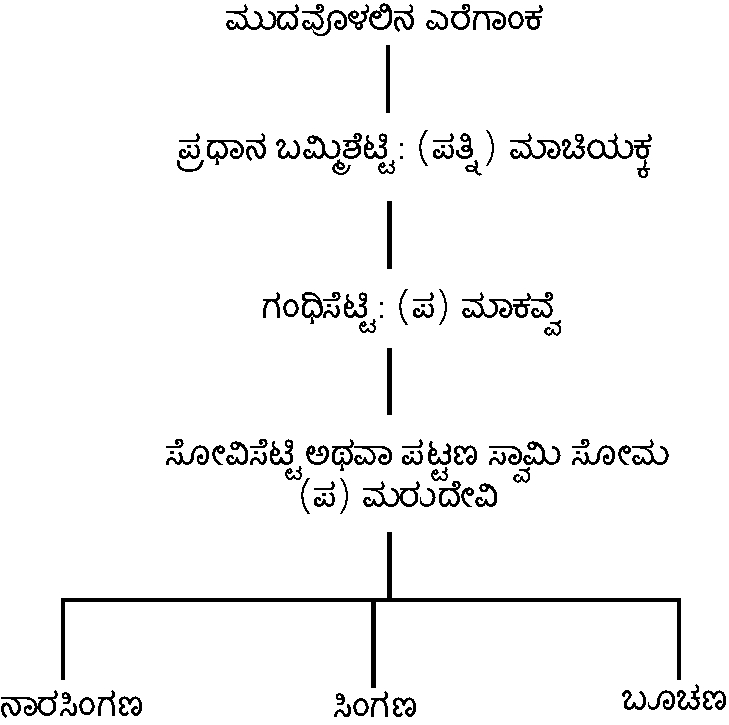
\includegraphics{images/chap8/chap8fig1.jpeg}
\end{figure}

\textbf{ಬೆಳ್ಳೂರಿನ ಪಟ್ಟಣಸ್ವಾಮಿ ಮಂಡಲಸ್ವಾಮಿ: }\index{ಪಟ್ಟಣಸ್ವಾಮಿ ಮಂಡಲಸ್ವಾಮಿ} ಬೆಳ್ಳೂರಿನ\index{ಬೆಳ್ಳೂರು} ಪಟ್ಟಣಸ್ವಾಮಿ ಮಂಡಲಸ್ವಾಮಿಯು\index{ಮಂಡಲಸ್ವಾಮಿ} ಬೆಳ್ಳೂರಿನಲ್ಲಿ\break \hbox{ಮಂಡಲೇಶ್ವರ} ದೇವಾಲಯ ಮತ್ತು ಕೆರೆಯನ್ನು ಕಟ್ಟಿಸಿ, ಬೆಳ್ಳೂರಿಗೆ ಸಮೀಪದಲ್ಲಿರುವ ಆರಣಿಯಲ್ಲಿ ಸಂತೆಯನ್ನು ಏರ್ಪಡಿಸಿ, ವ್ಯಾಪಾರಿಗಳು ವಿಶ್ರಮಿಸಿಕೊಳ್ಳಲು ಒಂದು ತಳ್ತಾರವೆಯನ್ನು\index{ತಳ್ತಾರವೆ} (ವಿಶ್ರಾಂತಿ ತಾಣ, ತಂಗುದಾಂಣ), ಊರಮುಂದೆ ಒಂದು ಕೆರೆಯನ್ನು, ನಿರ್ಮಿಸುತ್ತಾನೆ. ಮಂಡಲೇಶ್ವರ ದೇವರ\index{ಮಂಡಲೇಶ್ವರ ದೇವರ} ನಿವೇದ್ಯ, ಚೈತ್ರ ಪವಿತ್ರಕ್ಕೆ ಗದ್ದೆ ಬೆದ್ದಲುಗಳನ್ನು ಮಾಧವಜೀಯರಿಗೆ ದತ್ತಿಯಾಗಿ ಬಿಡುತ್ತಾನೆ.\endnote{ ಎಕ 7 ನಾಮಂ 80 ಬೆಳ್ಳೂರು 1199} ಶಾಸನವು ಮಂಡಲಸ್ವಾಮಿಯನ್ನು ಮತ್ತು ಅವನ ವಂಶವನ್ನು ಮನಸಾರೆ ಸ್ತುತಿಸಿದೆ.

ಮಂಡಲಸ್ವಾಮಿ ಎಂಬುದು ಪಟ್ಟಣಸ್ವಾಮಿಗಿಂತ ಉನ್ನತವಾದ ಹುದ್ದೆಯಂತೆ ಕಾಣುತ್ತದೆ. ಇವರದ್ದೂ ಪಟ್ಟಣ ಕಟ್ಟಿಸುವ, ಸಂತೆ ಕೂಡಿಸುವ ಕರ್ತವ್ಯ. ಇವರ ಸೇವೆ ಮಂಡಲವನ್ನು ವ್ಯಾಪಿಸಿತ್ತು ಎಂದು ಅಭಿಪ್ರಾಯ ಪಡಲಾಗಿದೆ.\endnote{ ಹಿರೇಮಠ್​, ಡಾ॥ ಬಿ.ಆರ್​., ಪೂರ್ವೋಕ್ತ, ಪುಟ 138-39} ಮಣ್ಡಲಸ್ವಾಮಿ ಸಾಮಿಶೆಟ್ಟಿ,\index{ಮಣ್ಡಲಸ್ವಾಮಿ ಸಾಮಿ} ಮಣ್ಡಲಸ್ವಾಮಿ ಮಲ್ಲಿಶೆಟ್ಟಿ,\index{ಮಣ್ಡಲಸ್ವಾಮಿ ಮಲ್ಲಿಶೆಟ್ಟಿ} ಇವರ ಹೆಸರುಗಳನ್ನು ನೋಡಿದರೆ, ಮಂಡಲಸ್ವಾಮಿ ಒಂದು ಹುದ್ದೆ ಎಂದು ಹೇಳಬಹುದು.\endnote{ ಎಕ 3 ನಂಗೂ 349 ತಗಡೂರು 13ನೇ ಶ.} ನಾನಾ ದೇಸಿಗರು ಆರವೆ\index{ಆರವೆ} ಮತ್ತು ಕೆರೆಗೆ ದತ್ತಿ ನೀಡಿರುವ ವಿಷಯ ಇತರ ಶಾಸನಗಳಿಂದಲೂ ತಿಳಿದುಬರುತ್ತದೆ. ಇದರಿಂದ ವ್ಯಾಪಾರಿಗಳು ವಿಶ್ರಾಂತ ತಾಣವಾದ ಆರವೆಗೆ ಮಹತ್ವ ನೀಡಿದ್ದರೆಂದು ಹೇಳಬಹುದು.\endnote{ ಎಕ 3 ನಂಗೂ 215 ಸುತ್ತೂರು 1032} ಬೆಳ್ಳೂರು ಶಾಸನದಿಂದ ಹೊರಡುವ ಮಂಡಲ ಸ್ವಾಮಿಯ ವಂಶಾವಳಿ ಈ ಕೆಳಗಿನಂತಿದೆ.

\begin{figure}[!h]
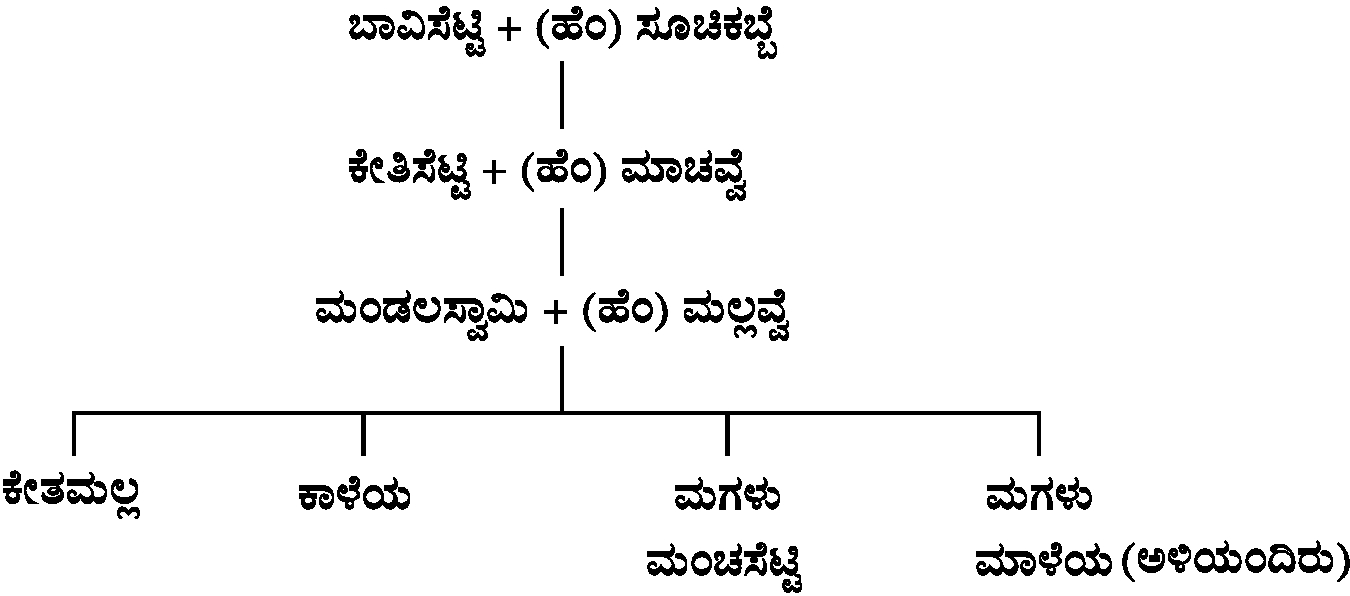
\includegraphics{images/chap8/chap8fig2.jpeg}
\end{figure}

ಬೆಳ್ಳೂರು ಕ್ರಿ.ಶ.1199ರ ಹೊತ್ತಿಗೆ ಒಂದು ಪಟ್ಟಣವಾಗಿತ್ತು. ಇಲ್ಲಿನ ಪಟ್ಟಣಸ್ವಾಮಿಯಾಗಿದ್ದ ಮಂಡಲಸ್ವಾಮಿಯು ಬೆಳ್ಳೂರಿಗೆ ಸಮೀಪದ ಆರಣಿಯಲ್ಲಿ ಸಂತೆಯನ್ನು\index{ಸಂತೆ} ಕಟ್ಟಿಸಿ ಅದನ್ನೂ ಕೂಡಾ ಪಟ್ಟಣವನ್ನಾಗಿ ಮಾಡಿದಂತೆ ತೋರುತ್ತದೆ. ಹೊಸ ಪಟ್ಟಣಗಳನ್ನು ಊರಿನಿಂದ ಹೊರಗೆ ರಚಿಸುತ್ತಿದ್ದರು ಎಂಬ ಅಭಿಪ್ರಾಯಕ್ಕೆ ಇದು ಪುಷ್ಟಿ ನೀಡುತ್ತದೆ. ಕ್ರಿ.ಶ.1270ರ ಹೊತ್ತಿಗೆ ಬೆಳ್ಳೂರು ಒಂದು ಅಗ್ರಹಾರವಾಯಿತು. ಆದರೂ ಅದು ಪಟ್ಟಣದ ಸ್ವರೂಪವನ್ನು ಹೊಂದಿತ್ತು. ಇಲ್ಲಿ ಪೆರುಮಾಳೆ ದೇವ ದಂಡನಾಯಕನು ದೇವಾಲಯಕ್ಕೆ ಸೇರಿದಂತೆ ಅಂಗಡಿಗಳನ್ನು ಕಟ್ಟಿಸಿ ಆ ದೇವರ ಅಂಗಡಿದೆರೆಯನ್ನು ದೇವರಿಗೆ ಮತ್ತು ಜೀವಿತವರ್ಗಕ್ಕೆ ದತ್ತಿಯಾಗಿ ಬಿಟ್ಟನು.\endnote{ ಎಕ 7 ನಾಮಂ 73 ಬೆಳ್ಳೂರು 1284} ಬೆಳ್ಳೂರ ಬಣಜಿಗರು ಬಹಳ ಪ್ರಸಿದ್ಧರಾಗಿದ್ದು ಅವರ ಬಗ್ಗೆ ಅನೇಕ ಜನಪದ ಗೀತೆಗಳಿವೆ.

\begin{verse}
\textbf{ಎಳ್ಳೂ ಕೊಳ್ಳೋಕೆ ಬೆಳ್ಳೂರ ಬಣಜಿಗ ಬಂದ} \\\textbf{ಎಳ್ಳುಂಟೆ ನಾರಿ ಹಣವೀವೆ। ಎನ್ನುತ} \\\textbf{ಬಳ್ಳ ಹಣಗೋಳ ಸುರಿದಾನು}
\end{verse}

\textbf{ನಾರಸಿಂಹಪಟ್ಟಣದ\index{ನಾರಸಿಂಹಪಟ್ಟಣ} ಬಲ್ಲಾಳುಸೆಟ್ಟಿ:\index{ಬಲ್ಲಾಳುಸೆಟ್ಟಿ} } ತೊಂಡನೂರು ಹಿರಿಯ ಅಗ್ರಹಾರದ ನಾರಸಿಂಹಪಟ್ಟಣದ ಬಲ್ಲಾಳುಸೆಟ್ಟಿಯು ಮಲ್ಲಿಕಾರ್ಜುನ ಶಿವಾಲಯದ ಹೊರಗೋಡೆಯನ್ನು ಕಟ್ಟಿಸಿದನೆಂದು ಕಾಚೇನಹಳ್ಳಿ\index{ಕಾಚೇನಹಳ್ಳಿ} ಶಾಸನದಲ್ಲಿ ಹೇಳಿದೆ.\endnote{ ಎಕ 6 ಪಾಂಪು 254 ಕಾಚೇನಹಳ್ಳಿ 12-13ನೇ ಶ.} ತೊಂಡನೂರು ಅಗ್ರಹಾರದ ಹೊರವಲಯದಲ್ಲಿ ಈ ಪಟ್ಟಣ ನಿರ್ಮಾಣವಾಗಿರಬಹುದು. ಕಾಚೇನಹಳ್ಳಿಯೇ ನಾರಸಿಂಹಪಟ್ಟಣವಾಗಿತ್ತು ಎಂದು ಊಹಿಸಬಹುದು. ಸಮೀಪದಲ್ಲಿ ದೇವರಾಯಪಟ್ಟಣವೆಂಬ ಊರೂ ಇದೆ.

\textbf{ತೆಲ್ಲಿಗರು:}\index{ತೆಲ್ಲಿಗರು} ಗ್ರಾಮ ಮತ್ತು ಪಟ್ಟಣಗಳಲ್ಲಿ ಎಣ್ಣೆ ಉತ್ಪಾದನೆ ಮಾಡುವವರು ತೆಲ್ಲಿಗರು. “ತೆಲ್ಲಿಗರು ಉತ್ಪಾದಕ ವಿನಿಮಯ ಸಂಘಕ್ಕೆ ಸೇರಿದವರು. ತೆಲ್ಲಿಗರೈವತ್ತೊಕ್ಕಲು ಇವರ ಸಂಘ. ಇವರ ಇನ್ನೊಂದು ಹೆಸರು ಗಾಣಿಗರು.\index{ಗಾಣಿಗರು} ಸಮಾಜದಲ್ಲಿ ಎಣ್ಣೆಗ ಅಧಿಕ ಬೇಡಿಕೆ ಇದ್ದ ಕಾರಣ ತೆಲ್ಲಿಗರು ಮಧ್ಯಯುಗ ಕರ್ನಾಟಕದ ಪ್ರಧಾನ ಘಟಕ”.\endnote{ ಹಿರೇಮಠ್​, ಡಾ॥ ಬಿ.ಆರ್​., ಪೂರ್ವೋಕ್ತ, ಪುಟ 103-104} ಕನ್ನಂಬಾಡಿ ಮಹಾ ಅಗ್ರಹಾರದ ಕಣ್ಣೇಶ್ವರ ದೇವರಿಗೆ ತೆಲಿಗ ಕೊತ್ತಳಿಯವರು ದತ್ತಿಯನ್ನು ಬಿಟ್ಟಿದ್ದಾರೆ. ಆದುದರಿಂದ ಇವರ ಸಂಘಕ್ಕೆ ಕೊತ್ತಳಿ ಎಂದೂ ಹೇಳುತ್ತಿದ್ದರೆಂದು ತಿಳಿದುಬರುತ್ತದೆ.\endnote{ ಎಕ 6 ಪಾಂಪು 35 ಕನ್ನಂಬಾಡಿ 12-13ನೇ ಶ.} ಕೆಲವು ಶಾಸನಗಳಲ್ಲಿ ತೆಲ್ಲಿಗ ಎಂದು ಹೇಳದೆ ಕೇವಲ ಸೆಟ್ಟಿ ಎಂದು ಹೇಳಿ ಅವನು ಗಾಣವನ್ನು ಮಾಡಿಸಿಕೊಟ್ಟಿದ್ದರೆ, ಅವರನ್ನು ತೆಲ್ಲಿಗರು ಎಂದು ಗುರುತಿಸಬೇಕಾಗುತ್ತದೆ. ಉದಾಹರಣೆಗೆ “ಶ‍್ರೀಮಾಚಿಸೆಟ್ಟಿ\index{ಮಾಚಿಸೆಟ್ಟಿ} ಮಾಡಿಸಿದ ಗಾಣಂ” ಎಂದು ತೊಳಸಿ(ಚಿ) ಶಾಸನದಲ್ಲಿ ಹೇಳಿದೆ.\endnote{ ಎಕ 6 ಕೃಪೇ 53 ತೊಣಚಿ 12ನೇ ಶ.} ತೆಲ್ಲಿಗ ಮಾರಗೌಡನ ಗಾಣದ ಸುಂಕದ ಉಲ್ಲೇಖವಿದ್ದು ತೆಲ್ಲಿಗರೂ ಗಾವುಂಡರಾಗಿದ್ದರೆಂದು ಊಹಿಸಬಹುದು.\endnote{ ಎಕ 6 ಕೃಪೇ 71 ಕಿಕ್ಕೇರಿ 1171} ಮಂಡ್ಯ ಜಿಲ್ಲೆಯ ಅನೇಕ ಹೊಯ್ಸಳ ದೇವಾಲಯಗಳ ಮುಂದೆ ಕಲ್ಲಿನ ಗಾಣಗಳನ್ನು ಇಂದಿಗೂ ನೋಡಬಹುದು.

\textbf{ಬಳಗಾರ ಕುಲ:}\index{ಬಳಗಾರ ಕುಲ} ವಿಶಿಷ್ಟ ಸರಕನ್ನು ಮಾರುವ ವರ್ತಕರನ್ನು ಶಾಸನಗಳು ಅದೇ ಹೆಸರಿನಿಂದ ಕರೆದಿವೆ ಎಂದು ಹೇಳಿ, ಅದಕ್ಕೆ ಬಳೆಗಾರ ಕೇಸವಸೆಟ್ಟಿ, ಬಳೆಗಾರ ಸರುವಯ್ಯಸೆಟ್ಟಿಯರನ್ನು ಉದಾಹರಣೆಯನ್ನಾಗಿ ನೀಡಲಾಗಿದೆ.\endnote{ ಹಿರೇಮಠ್​, ಡಾ॥ ಬಿ.ಆರ್​., ಪೂರ್ವೋಕ್ತ, ಪುಟ 20} ಬಳಗಾರ ಕುಲದ ಬಮ್ಮಣ್ಣ\index{ಬಮ್ಮಣ್ಣ} ಇಂಗಲೀಕನ ಕುಪ್ಪೆಯಲ್ಲಿ (ಇಂಗಳಗುಪ್ಪೆ) ಸ್ವಯಂಭು ದೇವಾಲಯವನ್ನು ಮತ್ತು ಕೆರೆಯನ್ನೂ ಕಟ್ಟಿಸುತ್ತಾನೆ.\endnote{ ಎಕ 6 ಪಾಂಪು 252 ತಿರುಮಲಸಾಗರ ಛತ್ರ, 1125} ಸುಜ್ಜಲೂರು ಬಳೆಗಾರ ಕೆಂಪಸೆಟ್ಟಿಯ ಮಗ ಸೋಯಿಸೆಟ್ಟಿ, ಬಳೆಗಾರ ಯರಗುಜೆಸೆಟ್ಟಿಯರು ಪಟ್ಟಣೀಕರಣದ ಪ್ರಕ್ರಿಯೆಯಲ್ಲಿ ಭಾಗವಹಿಸಿದ್ದಾರೆ.\endnote{ ಎಕ 7 ಮವ 136 ಸುಜ್ಜಲೂರು 1297} ಬಳಗಾರ ಕುಲ ಎಂಬುದು ಜೈನ ಬಲಾತ್ಕರ ಗಣ ಎಂದು ಹಂ.ಪ.ನಾ. ಅವರು ಹೇಳಿದ್ದಾರೆ.

\vskip 3pt

\textbf{ಮುನ್ನುರ್ವರು: }\index{ಮುನ್ನುರ್ವರು} ಉಗುರು ಮುನ್ನುರ್ವರು ಎಂಬ ವರ್ತಕ ಶ್ರೇಣಿ ಪ್ರಸಿದ್ಧವಾಗಿದೆ. ಉಗುರು ಮುನ್ನೂರ್ವರು, ಉಳಿಯ ಮುನ್ನೂರ್ವರು, ಕೊಯ್ಲಾಳಿಗಳು ಇವರು ವೀಳ್ಯದೆಲೆಯನ್ನು ಕೊಯ್ಯುವ ಕೆಲಸ ಮಾಡುವ ಆಳುಗಳು ಎಂದು ತಿಳಿದುಬರುತ್ತದೆ.\endnote{ ಹಿರೇಮಠ್​, ಡಾ॥ ಬಿ.ಆರ್​, ಪೂರ್ವೋಕ್ತ, ಪುಟ 99} ಕಿಕ್ಕೇರಿಯ ಬ್ರಹ್ಮೇಶ್ವರ ದೇವಾಲಯಕ್ಕೆ ಮುನ್ನೂರ್ವರು\index{ಮುನ್ನೂರ್ವರು} ದತ್ತಿ ಬಿಟ್ಟರೆಂದು ಹೇಳಿದೆ.\endnote{ ಎಕ 6 ಕೃಪೇ 27 ಕಿಕ್ಕೇರಿ 1171} ಇವರು ಉಗುರು ಮುನ್ನೂರ್ವರೇ\index{ಉಗುರು ಮುನ್ನೂರ್ವರು} ಇರಬಹುದು. ಅರಸಿಕೆರೆಯ ಒಂದು ಶಾಸನದಲ್ಲಿ “ಮೇಳೀಸಾಸಿರ್ವರು ನಾನಾದೇಶಿ ಮುಖ್ಯರಪ್ಪ ನಖರಮುಂ ಉಗುರುಮೂನೂರ್ವ್ವರು” ಎಂದು ಹೇಳಿದೆ.\endnote{ ಎಕ 10 ಅರ 44 ಅರಸಿಕೆರೆ 1189} ಉಗುರಕೆರೆ\index{ಉಗುರಕೆರೆ} ಎಂಬ ಒಂದು ಊರಿನ ಉಲ್ಲೇಖ ಕಿಕ್ಕೇರಿಗೆ ಸಮೀಪದ ಕಬ್ಬಳ್ಳಿಯ ಶಾಸನದಲ್ಲಿದೆ.\endnote{ ಎಕ 10 ಚರಾಪ 122 ಕಬ್ಬಳ್ಳಿ 1118} ಇದು ಉಗುರು ಮುನ್ನೂರ್ವರು ಪ್ರಧಾನವಾಗಿ ವಾಸಿಸುತ್ತಿದ್ದ ಊರಾಗಿರಬಹುದು.

\vskip 3pt

\textbf{ನಖರ:}\index{ನಖರ} ಇದೊಂದು ಸ್ಥಿರವಾದ ವರ್ತಕ ಸಂಘ. ನಗರಗಳಲ್ಲಿ ಹೆಚ್ಚಾಗಿ ಇರುತ್ತಿದ್ದರು.\endnote{ ಚಿದಾನಂದಮೂರ್ತಿ ಡಾ॥ ಎಂ., ಪೂರ್ವೋಕ್ತ, ಪುಟ 351} ಇವರನ್ನು ಅಂಗಡಿಸೆಟ್ಟಿಯವ\-ರೆಂದು ಕರೆದಿರುವುದರಿಂದ, ಸಂತೆ ಪಟ್ಟಣಗಳ ಸ್ಥಿರವಾದ ಅಂಗಡಿ ವ್ಯಾಪಾರಿಗಳಿವರೆಂದು ಹೇಳಬಹುದು.\endnote{ ಹಿರೇಮಠ, ಡಾ॥ ಬಿ.ಆರ್​., ಪೂರ್ವೋಕ್ತ, ಪುಟ 34} ಅರಸಿಕೆರೆ ಶಾಸನದಲ್ಲಿ “ಅಂಗಡಿಯ ನಖರುಂಗಳುಂ” ಎಂದು ಹೇಳಿದೆ.\endnote{ ಎಕ 10 ಅರ 44 ಅರಸಿಕೆರೆ 1189} ಇವರಲ್ಲಿ ಜೈನರು, ಶೈವರು ಇದ್ದರು. ಜೈನರು ನಖರ ಜಿನಾಲಯಗಳನ್ನು ಕಟ್ಟಿಸಿದರೆ, ಶೈವರು ನಖರೇಶ್ವರ ದೇವಾಲಯವನ್ನು ಕಟ್ಟಿಸುತ್ತಿದ್ದರು.\endnote{ ಹಿರೇಮಠ್​, ಡಾ॥ ಬಿ.ಆರ್​., ಪೂರ್ವೋಕ್ತ, ಪುಟ 75} ಮೊದಲಿಗೆ ಇವರು ಯಾವುದೇ ರೀತಿಯ ತೆರಿಗೆಗಳನ್ನು ನೀಡದೇ ವ್ಯಾಪಾರ ಮಾಡುತ್ತಿದ್ದುದರಿಂದ ಇದ್ದುದರಿಂದ ಇವರಿಗೆ ನ+ಕರ \textgreater  ನಖರ ಎಂದು ಹೆಸರು ಬಂದಿರಬಹುದು. ಇವರು ವ್ಯಾಪಾರಗಳನ್ನು ನಡೆಸುತ್ತಿದ್ದ ಊರುಗಳೇ ನಗರಗಳಾದವು ಎಂದು ಹೇಳಬಹುದು. ತೊಳಸಿಯ ನ(ಖ)ಗರೇಶ್ವರ ದೇವಾಲಯವನ್ನು ನಖರರು ನಿರ್ಮಿಸಿರಬಹುದು.\endnote{ ಎಕ 6 ಕೃಪೇ 50 ತೊಣಚಿ 104} ತೊಣಚಿ ಒಂದು ಪಟ್ಟಣವಾಗಿತ್ತು.\endnote{ ಎಕ 6 ಕೃಪೇ 56 ಭದ್ರನಕೊಪ್ಪಲು 12ನೇ ಶ.} ಕಿಕ್ಕೇರಿಯ ಬ್ರಹ್ಮೇಶ್ವರ ದೇವರಿಗೆ ಸಮಸ್ತ ನಖರ, ದೇಸಿ ಇಬ್ಬರೂ ಕೂಡಿ ದತ್ತಿ ಬಿಟ್ಟರೆಂದು ಹೇಳಿದೆ.\endnote{ ಎಕ 6 ಕೃಪೇ 27 ಕಿಕ್ಕೇರಿ. 1171} ಕಿಕ್ಕೇರಿಯು ಒಂದು ಪುರವಾಗಿದ್ದರಿಂದ ಇಲ್ಲಿ ನಖರರು ಇದ್ದರು. ತೊಂಡನೂರಿನ ಅಗ್ರಹಾರದ ಗಡಿಯಲ್ಲಿ ನಖರೇಶ್ವರ ದೇವಾಲಯ\index{ನಖರೇಶ್ವರ ದೇವಾಲಯ} ಇದ್ದಿತೆಂದೂ, ಅದಕ್ಕೆ ನಖರಂಗಳು ಹಾಗೂ ಸೆಟ್ಟಿಯರು ದತ್ತಿ ಬಿಟ್ಟರು ಎಂದು ಹೇಳಿದೆ.\endnote{ ಎಕ 6 ಪಾಂಪು 74 ತೊಣ್ಣೂರು 1189} ನಗರೂರ ಬೆಳ್ಳಿಯರು,\index{ನಗರೂರ ಬೆಳ್ಳಿಯರು}\endnote{ ಎಕ 7 ಮಂ 14 ಹುಳ್ಳೇನಹಳ್ಳಿ 8ನೇ ಶ.} ನಗರೂರ ಸೋಮಯ್ಯ,\index{ನಗರೂರ ಸೋಮಯ್ಯ}\endnote{ ಎಕ 7 ಮ 104 ಹಾಗಲಹಳ್ಳಿ 11-12ನೇ ಶ.} ನಗರೂರ ಗುತ್ತಿಯನಾಯಕನ ಮಗ ಜಕ್ಕಂಣ ನಾಯಕ\endnote{ ಎಕ 7 ಮಂ 17 ದುದ್ದ 1596} ಇವರ ಉಲ್ಲೇಖ ಜಿಲ್ಲೆಯ ಶಾಸನಗಳಲ್ಲಿ ಕಂಡುಬರುತ್ತದೆ. ಸಿಂದಘಟ್ಟದ ಸಮೀಪ ಇದ್ದ ನಗರೂರಿನ ಉಲ್ಲೇಖ ತೊಣ್ಣೂರು\endnote{ ಎಕ 6 ಪಾಂಪು 88 ತೊಣ್ಣೂರು 1157} ಮತ್ತು ಕೈಗೋನಹಳ್ಳಿ ಶಾಸನಗಳಲ್ಲಿ\endnote{ ಎಕ 6 ಕೃಪೇ 71 ಕೈಗೋನಹಳ್ಳಿ 1462} ಬಂದಿದೆ. ಇವೆಲ್ಲಾ ನಖರರು ವಾಸಿಸುತ್ತಿದ್ದ ಊರುಗಳಾಗಿರಬಹುದು. “ರಾಜರಾಜಪುರವಾದ ಏಳುಪುರದ ಪಂಚಮಠದ ನಖರ ಸ್ಥಾನಪತಿಗಳ”\index{ನಖರ ಸ್ಥಾನಪತಿಗಳು} ಉಲ್ಲೇಖ ಬಸವನಪುರ,\endnote{ ಎಕ 7 ಮವ 43 ಬಸವನಪುರ 1513} ಚಂದಹಳ್ಳಿ,\endnote{ ಎಕ 7 ಮವ 81 ಚಂದಹಳ್ಳಿ 14ನೇ ಶ.} ಶಾಸನಗಳಲ್ಲಿದೆ. ಈ ಶಾಸನಗಳಲ್ಲಿ ಹಳ್ಳಿಗಳನ್ನು ಪುರವನ್ನಾಗಿ ಮಾಡುವುದರ ವಿಷಯ ಇರುವುದರಿಂದ ಈ ಮಠಗಳು ನಖರ ಸಮೂಹಕ್ಕೆ ಸಂಬಂಧಿಸಿದ್ದಿರಬಹುದು. ಮೈಸೂರು ಸಂಸ್ಥಾನದ ಪೇಟೆನಾಡದೇಶದ ನಗರತರ ಚನ್ನಯ್ಯನ ಉಲ್ಲೇಖವಿದೆ. \endnote{ ಎಕ 7 ನಾಮಂ 180 ಹೊಣಕೆರೆ 19ನೇ ಶ.} ಈಗ ನಗರ್ತ ಶಿವಾಚಾರ ವೈಶ್ಯ\index{ನಗರ್ತ ಶಿವಾಚಾರ ವೈಶ್ಯ} ಎಂಬ ಜನಾಂಗವಿದೆ.

\vskip 3pt

\textbf{ಗವರೆ:}\index{ಗವರೆ} ಇವರು ಕತ್ತೆ ಮೊದಲಾದ ಪ್ರಾಣಿಗಳ ಮೇಲೆ ವೀಳ್ಳೆಯದೆಲೆಗಳನ್ನು ಹೇರಿಕೊಂಡು ಊರಿಂದೂರಿಗೆ ಪ್ರಯಾಣ ಮಾಡುತ್ತಾ ವ್ಯಾಪಾರ ಮಾಡುತ್ತಿದ್ದರು. ಇವರನ್ನು ಗವರೆಸೆಟ್ಟಿ\index{ಗವರೆಸೆಟ್ಟಿ} ಎಂದೂ ಕರೆಯಲಾಗಿದೆ.\endnote{ ಹಿರೇಮಠ್​, ಡಾ॥ ಬಿ.ಆರ್​., ಪೂರ್ವೋಕ್ತ, ಪುಟ 59} ಅಯ್ಯಾವೊಳೆ ಐನೂರ್ವರ ಸಂಘದ ವರ್ತಕರು ಧನಗೂರಿನಲ್ಲಿ ಗವರೈ ಈಶ್ವರ ಮುಡೈಯಾರ್​\index{ಗವರೈ ಈಶ್ವರ ಮುಡೈಯಾರ್​}(ಗವರೇಶ್ವರ) ದೇವಾಲಯವನ್ನು ಕಟ್ಟಿಸಿ ದತ್ತಿ ಬಿಟ್ಟ ವಿಚಾರ ಇದೆ.\endnote{ ಎಕ 7 ಮವ 51 ಧನಗೂರು 13ನೇ ಶ.} ಇವರು ಗವರೆಗಳಾಗಿದ್ದು, ಅಯ್ಯಾವೊಳೆ ಐನೂರ್ವರು ಸಂಘದ ಪರಂಪರೆಯವರೆಂದು ಹೇಳಬಹುದು. ಬೇಡರ ಪಡೆಯು ನಡೆಸಿದ ಪೆಂಡಿರುಡೆಯುರ್ಚಿನಲ್ಲಿ, ಹೋರಾಡಿ ಮಡಿದ ಗವರೆಸೆಟ್ಟಿಯನ್ನು ಗವರೆ ಕುಲ ತಿಲಕ\index{ಗವರೆ ಕುಲ ತಿಲಕ} ಎಂದು ಶಾಸನ ಹೊಗಳಿದೆ. ಬೆಳ್ಳೂರಿನಲ್ಲಿ ಮಂಡಲಸ್ವಾಮಿ ಕಟ್ಟಿಸಿದ ದೇವಾಲಯವನ್ನು ಸ್ಥಳೀಯರು ಗವರೇಶ್ವರ ದೇವಾಲಯವೆಂದು ಹೇಳುತ್ತಾರೆ.

\vskip 3pt

\textbf{ವಡ್ಡವ್ಯವಹಾರಿ/ಮಹಾವಡ್ಡವ್ಯವಹಾರಿ:} “ಪ್ರಾಚೀನ ಮತ್ತು ಮಧ್ಯಕಾಲೀನ ಕರ್ನಾಟಕದ ವರ್ತಕ ಪ್ರಕಾರಗಳಲ್ಲಿ ವಡ್ಡವ್ಯವಹಾರಿ ಅತ್ಯಂತ ಪ್ರಮುಖವಾದುದು. ವಡ್ಡವ್ಯವಹಾರಿಗಳಲ್ಲೇ ಹಿರಿಯ ವರ್ತಕನಾದವನಿಗೆ ಮಹಾವಡ್ಡವ್ಯವಹಾರಿ ಎಂದು ಹೇಳುತ್ತಿದ್ದರು. ಇವರು ಸಾಮಂತರ ಪಾದಪದ್ಮೋಪಜೀವಿಗಳಾಗಿದ್ದು ರಾಜ್ಯಾಡಳಿತ ನಡೆಸುತ್ತಿದ್ದಂತೆ ಕಂಡು ಬರುತ್ತದೆ. ಇವರು ಸೆಟ್ಟಿ ಎಂಬ ಕುಟುಂಬಕ್ಕೆ ಸೇರಿದವರು”.\endnote{ ಹಿರೇಮಠ್​ ಡಾ॥ ಬಿ.ಆರ್​., ಪೂರ್ವೋಕ್ತ, ಪುಟ 49-50}

ಅರಸಿಕೆರೆ ತಾಲ್ಲೂಕು ಹಿರಿಯೂರಿನ ಶಾಸನದಲ್ಲಿ ಮಹಾವಡ್ಡವ್ಯವಹಾರಿಗಳ ಪ್ರಶಸ್ತಿ ಇದೆ.\endnote{ ಎಕ 10 ಅರ 317 ಹಿರಿಯೂರು 1254} ಕಿಕ್ಕೇರಿಯ ಬ್ರಹ್ಮೇಶ್ವರ ದೇವರಿಗೆ ದತ್ತಿ ಬಿಟ್ಟಾಗ ಅಲ್ಲಿ ಶ‍್ರೀಮನು ಮಹಾವಡ್ಡವ್ಯವಹಾರಿ ಪಟ್ಟಣಸ್ವಾಮಿ ಇದ್ದನೆಂದು ಹೇಳಿದೆ. ಇದರಿಂದ ಮಹಾ ವಡ್ಡವ್ಯವಹಾರಿಗಳೂ ಪಟ್ಟಣಸ್ವಾಮಿಗಳಾಗಿರುತ್ತಿದ್ದರೆಂದು ಹೇಳಬಹುದು.\endnote{ ಎಕ 6 ಕೃಪೇ 27 ಕಿಕ್ಕೇರಿ 1171} ಶ‍್ರೀಮನ್​ ಮಹಾವಡ್ಡ ವ್ಯವಹಾರಿ ಕೆಂಚಗಾರಸೆಟ್ಟಿ ಮತ್ತು ಹಾಜನಂಬಿ ಇವರು ಅಂತರವಳ್ಳಿಯ ರಾಮೇಶ್ವರ ದೇವರಿಗೆ ದತ್ತಿ ಬಿಡುತ್ತಾರೆ.\endnote{ ಎಕ 7 ಮವ 33 ಅಂತರವಳ್ಳಿ 1262} ಮುಮ್ಮಡಿ ಬಲ್ಲಾಳನ ಮಹಾಪ್ರಧಾನ ಆದಿಸಿಂಗೆಯ ದಂಡನಾಯಕನು, ಬಹುಶಃ ನಾಡಮಾಣಿಕದೊಡಲೂರಿನ ಬಸದಿಗೆ ಸೇರಿದ್ದ, ಕಲ್ಲಹಳ್ಳಿಯನ್ನು ದೇವಲಾಪುರವೆಂಬ ಅಗ್ರಹಾರವನ್ನಾಗಿ ಮಾಡಿದಾಗ ಅಲ್ಲಿ ಜೈನ ರಾಜಗುರುಗಳ ಜೊತೆಗೆ, ಶ‍್ರೀಮನುಮಹಾವಡ್ಡವ್ಯವಹಾರಿ ಉಭಯ ನಾನಾದೇಶಿ ನಾಗಮಲ್ಲಿದೇವ\index{ಉಭಯ ನಾನಾದೇಶಿ ನಾಗಮಲ್ಲಿದೇವ} ಪದುಮನಾಯಕರ ಮಕ್ಕಳು ದಾಮೋದರನಾಯಕರು, ಶ‍್ರೀಮನುಮಹಾ ವಡ್ಡವ್ಯವಹಾರಿ\index{ಮಹಾ ವಡ್ಡವ್ಯವಹಾರಿ ನಾಗಯ್ಯ} ನಾಗಯ್ಯಗಳ ಮಕ್ಕಳು ನಾಗದೇವರಸರು, ಶ‍್ರೀಮನುಮಹಾ ವಡ್ಡವ್ಯವಹಾರಿ\index{ಮಹಾ ವಡ್ಡವ್ಯವಹಾರಿ} ಮುದನೂರ ಕೇಸವನಾಯಕರುಗಳ\break ಉಭಯಾನುಮತದಿಂದ ಶಾಸನವನ್ನು ಹಾಕಲಾಯಿತೆಂದು ವರಾಹನಾಥ ಕಲ್ಲಹಳ್ಳಿ ಶಾಸನದಲ್ಲಿ ಹೇಳಿದೆ. ಈ ರೀತಿಯ ವ್ಯವಹಾರಗಳಲ್ಲಿ ಮಹಾವಡ್ಡ ವ್ಯವಹಾರಿಗಳು ಪ್ರಮುಖ ಪಾತ್ರ ವಹಿಸುತ್ತಿದ್ದರೆಂದು ಹೇಳಬಹುದು.\endnote{ ಎಕ 6 ಕೃಪೇ 108 ವರಾಹನಾಥಕಲ್ಲಹಳ್ಳಿ 1334} ಕಣಿಕಟ್ಟೆಯಲ್ಲಿ ಸ್ಥಾನಪತಿಗಳಿಗೂ ಮಹಾಜನರಿಗೂ ಭೂಮಿಯ ವಿಚಾರದಲ್ಲಿ ವಿವಾದ ಉಂಟಾದಾಗ ಅದನ್ನು ಬಗೆಹರಿಸುವಾಗಲೂ ಮಹಾವಡ್ಡ\-ವ್ಯವಹಾರಿಗಳು ಪ್ರಮುಖ ಪಾತ್ರ ವಹಿಸಿರುವುದು ಕಂಡು ಬರುತ್ತದೆ.\endnote{ ಎಕ 10 ಅರ 89 ಕಣಿಕಟ್ಟೆ 1274}

\section*{ಪಟ್ಟಣೀಕರಣ}
\index{ಪಟ್ಟಣೀಕರಣ}

“ಸಂತೆ\index{ಸಂತೆ} ಮಾಡಿಸುವುದರಿಂದ ಗ್ರಾಮ ಪಟ್ಟಣವೆನಿಸುತ್ತಿದ್ದಿತು. ಇದರಿಂದ ಮಧ್ಯಕಾಲೀನ ಕರ್ನಾಟಕದ ಪ್ರತಿಯೊಂದು ಪಟ್ಟಣದಲ್ಲಿಯೂ ಸಂತೆ ಜರುಗುತ್ತಿದ್ದುದು ತಿಳಿಯುತ್ತದೆ. ಕೆಲವು ಸಲ ಸಂತೆ ಕಟ್ಟಿಸಿ ಗ್ರಾಮವನ್ನೇ ಪಟ್ಟಣವನ್ನಾಗಿ ಪರಿವರ್ತಿಸು\-ತ್ತಿದ್ದರು. ಹೊಸದಾಗಿ ನಿರ್ಮಿಸಿದ ಪಟ್ಟಣ ಮೂಲಗ್ರಾಮದಿಂದ ಪ್ರತ್ಯೇಕವಾಗಿರುತ್ತಿತ್ತು. ಊರನ್ನೇ ಪಟ್ಟಣವನ್ನಾಗಿ ಪರಿವರ್ತಿಸಿದಾಗ ಈ ಪ್ರಶ್ನೆ ಉದ್ಭವಿಸಲಾರದು.”\endnote{ ಹಿರೇಮಠ್​ ಡಾ॥ ಬಿ.ಆರ್​, ಪೂವೋಕ್ತ, ಪುಟ 118-119} ಪಟ್ಟಣಸೆಟ್ಟಿಗಳು, ಮಹಾವಡ್ಡವ್ಯವಹಾರಿಗಳು, ಅಧಿಕಾರಿಗಳು ಈ ಪಟ್ಟಣೀಕರಣದಲ್ಲಿ ಮುಖ್ಯಪಾತ್ರ ವಹಿಸುತ್ತಿದ್ದರು.

“ಹೊಯ್ಸಳ ಸಾಮ್ರಾಜ್ಯದಲ್ಲಿ ಆರ್ಥಿಕ ಪರಿಸ್ಥಿತಿ ಬಹಳ ಉತ್ತಮಮಟ್ಟದ್ದು ಹಾಗೂ ಸುಭದ್ರವೂ ಆಗಿದ್ದಿತು. ವಾಣಿಜ್ಯ ವ್ಯವಹಾರಗಳು ಸುಗಮವಾಗಿ ದೊಡ್ಡಪ್ರಮಾಣದಲ್ಲಿ ನಡೆಯುತ್ತಿದ್ದವು. ಈ ಕಾರಣದಿಂದಾಗಿ ಹೊಯ್ಸಳ ಸಾಮ್ರಾಜ್ಯದಲ್ಲಿ ನಗರ ವ್ಯವಸ್ಥೆ ಅಥವಾ ಪಟ್ಟಣೀಕರಣವು ವಿಶೇಷವಾಗಿ ತ್ವರಿತಗತಿಯಲ್ಲಿ ನಡೆಯಿತು. ನಗರಗಳನ್ನು ಪಟ್ಟಣ, ಪುರ, ವೀಡು ಎಂದು ಕರೆಯುಲಾಗಿದೆ. ಈ ನಗರ ಕೇಂದ್ರಗಳ ಬೆಳವಣಿಗೆಗೆ ವಾಣಿಜ್ಯ ವ್ಯವಹಾರಗಳಷ್ಟೇ ಸಂಸ್ಕೃತಿ ಹಾಗೂ ರಾಜ್ಯತಂತ್ರಗಳೂ ಕಾರಣ”.\endnote{ ಕರ್ನಾಟಕ ಚರಿತ್ರೆ, ಹಂಪಿ ಕನ್ನಡ ವಿವಿ, ಸಂಪುಟ 2, ಪುಟ 201-211} ಪಟ್ಟಣೀಕರಣವು ವಿಜಯನಗರ ಕಾಲದಲ್ಲೂ ಮುಂದುವರಿಯಿತು.

ನಗರ, ಪಟ್ಟಣ, ಪುರಗಳಲ್ಲಿ ಬೃಹತ್​ ದೇವಾಲಯಗಳನ್ನು, ಅನ್ನಸತ್ರ, ಪಾಠಶಾಲೆ, ಬ್ರಹ್ಮಪುರಿ, ಘಟಿಕಾಸ್ಥಾನಗಳನ್ನು ನಿರ್ಮಿಸುತ್ತಿದ್ದುದು ನಗರೀಕರಣಕ್ಕಿರುವ ಸಾಂಸ್ಕೃತಿಕ ಹಿನ್ನೆಲೆಯನ್ನು ತೋರಿಸುತ್ತದೆ. ಕೆಲವೆಡೆ ದೇವಾಲಯವನ್ನು ನಿರ್ಮಿಸಿ ನಂತರ ಆ ಊರನ್ನು ಪಟ್ಟಣವನ್ನಾಗಿ ಮಾಡಲಾಗುತ್ತಿತ್ತು. ಅಥವಾ ಅದು ಪಟ್ಟಣವಾಗಿ ಬೆಳೆಯುತ್ತಿತು. ಪಟ್ಟಣಗಳಲ್ಲಿ ಖಾಯಂ ಅಂಗಡಿಗಳು, ಅಂಗಡಿಸಾಲು ಇರುತ್ತಿತ್ತು. ದೇವಾಲಯಕ್ಕೆ ಸೇರಿದಂತೆಯೂ ಅಂಗಡಿಗಳನ್ನು ಕಟ್ಟಿ ಅವುಗಳಿಗೆ ತೆರಿಗೆಯನ್ನು ಅಥವಾ ಬಾಡಿಗೆಯನ್ನು ವಿಧಿಸಲಾಗುತ್ತಿತು.

ಗಂಗರ ಕಾಲದಲ್ಲಿ ರಾಜಧಾನಿಗಳು, ಧಾರ್ಮಿಕ ಕೇಂದ್ರಗಳು, ಪಟ್ಟಣಗಳಾಗಿದ್ದವೆಂದು ಹೇಳಬಹುದು. ಗಂಗರು ತಮ್ಮನ್ನು ಕುವಳಾಲ(ಕೊವಳಾಲ)ಪುರವರಾಧೀಶ್ವರರೆಂದು ಹೇಳಿಕೊಂಡಿದ್ದಾರೆ. ತಲಕಾಡನ್ನು ತಲವನಪುರ, ವಿಜಯಸ್ಕನ್ದಾವಾರ ಎಂದು ಹೇಳಿದೆ.\endnote{ ಎಕ 7 ಮಂ 35 ಹಳ್ಳೆಗೆರೆ 713} ಅದೇ ರೀತಿ ಶ‍್ರೀವುರದಲ್ಲಿ ಲೋಕತಿಲಕ ಭವನವೆಂಬ ಬಸದಿಯನ್ನು ನಿರ್ಮಿಸಲಾಯಿತೆಂದು ಹೇಳಿದೆ.\endnote{ ಎಕ 7 ನಾಮಂ 149 ದೇವರಹಳ್ಳಿ 776} ತಲಕಾಡಿಗೆ ಶ‍್ರೀಪುರವೆಂಬ\index{ಶ‍್ರೀಪುರ} ಹೆಸರಿತ್ತೆಂದು ಹೇಳಬಹುದು. ಶ‍್ರೀರಂಗಪಟ್ಟಣಕ್ಕೆ ಶ‍್ರೀವುರಮಂಗಲವೆಂಬ\index{ಶ‍್ರೀವುರ ಮಂಗಲ} ಹೆಸರಿತ್ತು. ಇಲ್ಲಿಯೂ ದೇವಾಲಯಗಳು, ಬಸದಿಗಳು ಇದ್ದವು. ಹೊಯ್ಸಳರ ಶಾಸನಗಳಲ್ಲಿ ತಳಕಾಡು, \endnote{ ಎಕ 6 ಕೃಪೇ 50 ತೊಣಚಿ 1048} ತೊಳಂಚೆಯನ್ನು\endnote{ ಎಕ 6 ಕೃಪೇ 56 ಭದ್ರನಕೊಪ್ಪಲು 1120} ಪಟ್ಟಣವೆಂದು ಹೇಳಿದೆ. ಹೊಯ್ಸಳರ ಶಾಸನಗಳಲ್ಲಿ ಹದಿನೆಂಟು ಪಟ್ಟಣದ ಉಲ್ಲೇಖವಿದೆ.\endnote{ ಎಕ 7 ಮವ 51 ಧನಗೂರು, ಮವ 54 ಮಾರೆಹಳ್ಳಿ 13ನೇ ಶ.} ಇವು ಹೊಯ್ಸಳ ಸಾಮ್ರಾಜ್ಯದಲ್ಲಿದ್ದ ಹದಿನೆಂಟು ಪಟ್ಟಣಗಳಾಗಿರಬಹುದು.

ಕೌಶಿಕ ಕುಲದ ವಿಭು ದೇವರಾಜನು ವಿಷ್ಣುವರ್ಧನನಿಂದ ಸೂರನಹಳ್ಳಿಯನ್ನು ದತ್ತಿಯಾಗಿ ಪಡೆದು ಅಲ್ಲಿ ಪಾರ್ಶ್ವನಾಥ ಜಿನಗೇಹವನ್ನು ಕಟ್ಟಿಸಿ ಅದನ್ನು ಪಾರ್ಶ್ವಪುರವನ್ನಾಗಿ\index{ಪಾರ್ಶ್ವಪುರ} ಮಾಡುತ್ತಾನೆ. ಇದಕ್ಕಾಗಿ ಅವನಿಗೆ ಆ ಊರಿನ ಮೊದಲ ನಾಲ್ವತ್ತು ಹೊನ್ನಿನೊಳಗೆ ಹತ್ತು ಹೊನ್ನನ್ನು ನೀಡಲಾಗುತ್ತದೆ.\endnote{ ಎಕ 7 ನಾಮಂ 64 ಯಲ್ಲಾದಹಳ್ಳಿ 1145} ಸೋಮಯ್ಯನೆಂಬ ಅಧಿಕಾರಿಯು ನಾಡಮಾಣಿಕದೊಡಲೂರನ್ನು ಶ‍್ರೀಮತ್​ ಮಾಣಿಕ್ಯ ಪೊಳಲನ್ನಾಗಿ ಮಾಡಿ ಅಲ್ಲಿದ್ದ ಹೊಯ್ಸಳ ಜಿನಾಲಯಕ್ಕೆ ದತ್ತಿಗಳನ್ನು ಬಿಡುತ್ತಾನೆ.\endnote{ ಎಕ 6 ಕೃಪೇ 106 ಬಸ್ತಿ 1165}

ವಿನಯಾದಿತ್ಯನ ಕಾಲದಲ್ಲಿ ಕ್ರಿ.ಶ. 1095ರಲ್ಲಿ ಕಿಕ್ಕೇರಿಯ ಕೆರೆಯ ಬಳಿ ಮೂಲ ಬ್ರಹ್ಮೇಶ್ವರ ದೇವಾಲಯವಿತ್ತು. ಆದರೆ ಬೊಮ್ಮವ್ವೆಯು ಒಂದನೇ ನರಸಿಂಹನ ಕಾಲದಲ್ಲಿ, (1171) ಊರಿಗೆ ಹೊಂದಿಕೊಂಡ ಹಾಗೆ ಹಿರಿಕೆರೆಯ ಬಳಿ ಬ್ರಹ್ಮೇಶ್ವರ ದೇವಾಲಯವನ್ನು ನಿರ್ಮಿಸಿದಳು. ಈ ಶಾಸನದಲ್ಲಿ ಕಿಕ್ಕೇರಿಯನ್ನು ಪುರ, ವೀಡು ಎಂದು ಹೇಳಿದೆ. ದೇವಾಲಯ ನಿರ್ಮಾಣದ ನಂತರ ಈ ಊರು ಪಟ್ಟಣವಾಗಿ ಬೆಳೆಯತೊಡಗಿತು. ಈ ಪುರದಲ್ಲಿ ಸಮಸ್ತ ನಖರ, ದೇಸಿ, ಮುನೂರ್ವ್ವರು, ತೆಲ್ಲಿಗರು,\index{ತೆಲ್ಲಿಗರು} ಸುಂಕದ ಅಧಿಕಾರಿಗಳು ಇದ್ದರು.

ಜೈನತೀರ್ಥವಾಗಿದ್ದ ತಿಪ್ಪೂರನ್ನು ಪಟ್ಟಣವನ್ನಾಗಿ ಮಾಡಲು ತಿಪ್ಪೂರ ಪಟ್ಟಣಸ್ವಾಮಿ ಚೆಟ್ಟಿಸೆಟ್ಟಿಯರ\index{ತಿಪ್ಪೂರ ಪಟ್ಟಣಸ್ವಾಮಿ ಚೆಟ್ಟಿಸೆಟ್ಟಿ} ಮಗ ಪರಡಿಸೆಟ್ಟಿ, ನಕರಸೆಟ್ಟಿ, ಪಟ್ಟಣಸ್ವಾಮಿ ಚಕ್ರವರ್ತಿಯ ಮಗ ಅಂತಪ್ಪ ಇವರಿಗೆ ಗದ್ದೆ ಬೆದ್ದಲುಗಳನ್ನು, ಮನೆಯನ್ನು ಅನೇಕ ತೆರಿಗೆಗಳನ್ನು ದತ್ತಿಯಾಗಿ ಬಿಡಲಾಗಿದೆ.\endnote{ ಎಕ 7 ಮ 52 ತಿಪ್ಪೂರು 12ನೇ ಶ.} ಈ ಶಾಸನದಲ್ಲಿ ಹಿರಿಯಕಟ್ಟಣಗೆರೆ, ಚಿಕ್ಕಕಟ್ಟಣಗೆರೆಗಳ ಉಲ್ಲೇಖವಿದ್ದು, ಈ ಹಳ್ಳಿಗಳೂ ಕೂಡಾ ತಿಪ್ಪೂರು ಪಟ್ಟಣದ ವ್ಯಾಪ್ತಿಗೆ ಬರುತ್ತಿದ್ದವೆಂದು ಹೇಳಬಹುದು\endnote{ ಕರ್ನಾಟಕ ಚರಿತ್ರೆ, ಸಂಪುಟ 2, ಕನ್ನಡ ವಿವಿ ಹಂಪಿ, ಪುಟ 203} ಚಿಕ್ಕಕಟ್ಟಣಗೆರೆಯ ಪಟ್ಟಣಸ್ವಾಮಿಗೆ, ಜಿನಾರ್ಚನೆಗೆ ಗದ್ದೆಯನ್ನು ದತ್ತಿಬಿಡಲಾಗಿದೆ.\endnote{ ಎಕ 7 ಮ 52 ತಿಪ್ಪೂರು 12ನೇ ಶ.}

ಎಂಮದೂರ ಹಳ್ಳಿಯನ್ನು (ಮಳವಳ್ಳಿ ತಾ. ಯಮ್ಮದೂರು) ಪಟ್ಟಣವನ್ನಾಗಿ ಬಳಗಾರ ಮಲ್ಲಪ್ಪಸೆಟ್ಟಿಯಾದ\index{ಬಳಗಾರ ಮಲ್ಲಪ್ಪಸೆಟ್ಟಿ} ಹಸಿಯಪ್ಪಂಗೆ ಎಂಮದೂರ ಸಮಸ್ತ ಗವುಡುಗಳು ಕೂಡಿ, ಮೊದಲು (ಮೊದಲ ಸಂವತ್ಸರ) 32 ಗದ್ಯಾಣವನ್ನು ನೀಡುತ್ತಾರೆ. ಅಲ್ಲಿಂದ ಮೇಲೆ ಅಳಿವು ಅನ್ಯಾಯವೆಂಬ ತೆರಿಗೆಯನ್ನು ಮಾತ್ರ ಕಟ್ಟುಗುತ್ತಗೆ ಮತ್ತು ಪಿಂಡಾದಾನವಾಗಿ ಪಟ್ಟಣಕ್ಕೆ ಒಡಂಬಟ್ಟು ತೆರಲು ಒಪ್ಪಿಕೊಂಡು ಕರಾರು ಮಾಡಿಕೊಳ್ಳುತ್ತಾರೆ. ಆ ಹಳ್ಳಿಯ ಎಲ್ಲೆಯೇ ಪಟ್ಟಣದ ಎಲ್ಲೆ ಎಂದು ಗುರುತಿಸಲಾಗಿದೆ.\endnote{ ಎಕ 7 ಮಂ 71 ಕನ್ನಲ್ಲಿ 1251}

ಗವುಡುಗೆರೆಯ (ಮಳವಳ್ಳಿ ತಾ. ಗೌಡಗೆರೆ) ಪಟ್ಟಣಸ್ವಾಮಿಗಳು\index{ಪಟ್ಟಣಸ್ವಾಮಿ} ಮಯಿದಸೆಟ್ಟಿಯ\index{ಮಯಿದಸೆಟ್ಟಿ} ತಮ್ಮ ತಿವಡಿಸೆಟ್ಟಿ,\index{ತಿವಡಿಸೆಟ್ಟಿ} ಕೇತಿಸೆಟ್ಟಿ,\index{ಕೇತಿಸೆಟ್ಟಿ} ಬೂಕಿಸೆಟ್ಟಿ, ಸಿದ್ದಂಣ.... ಸೆಟ್ಟಿ ಇವರೊಳಗಾದ ಪಟ್ಟಣಸ್ವಾಮಿಗಳಿಗೆ ವೀರಸೋಮೇಶ್ವರನು ದೇವಮಾನ್ಯವಾಗಿ ಗದ್ದೆಬೆದ್ದಲುಗಳನ್ನು ನೀಡಿ, ಕೆಲವು ತೆರಿಗೆಗಳನ್ನು ಬಿಟ್ಟನೆಂದು ಹೇಳಿದೆ.\endnote{ ಎಕ 7 ಮವ 23 ಗೌಡಗೆರೆ 1253} ಬಹುಶಃ ಗವುಡುಗೆರೆಯಲ್ಲಿ ಸಂತೆಯನ್ನು ಕಟ್ಟಿಸಿ ಪಟ್ಟಣವನ್ನಾಗಿ ಮಾಡಲು ಈ ದತ್ತಿಗಳನ್ನು ನೀಡಿರಬಹುದು. ಗಾವುಂಡರೂ ಸಹ ಪಟ್ಟಣಸ್ವಾಮಿಗಳ ಜೊತೆ ಕಾರ್ಯವನ್ನು ನಿರ್ವಹಿಸುತ್ತಿದ್ದರೆಂದು ಹೇಳಬಹುದು. “ಸಂತೆಯನ್ನು ಗೌಡ, ಮಹಾಪ್ರಭು ವರ್ತಕ ಮೊದಲಾದವರು ಸೇರಿ ನೆರೆಯಿಸುತ್ತಿದ್ದರು”,\endnote{ ಹಿರೇಮಠ್​, ಡಾ॥ ಬಿ.ಆರ್​., ಪೂರ್ವೋಕ್ತ, ಪುಟ 114-15} ಎಂದು ತಿಳಿದುಬರುತ್ತದೆ.

ತುಗಿಲೂರ ಹಳ್ಳಿಯನ್ನು (ಮಳವಳ್ಳಿ ತಾ. ಸುಜ್ಜಲೂರು) ಮಾಧವಪಟ್ಟಣವನ್ನಾಗಿ ಮಾಡಲು ಬಳೆಗಾರ ಕೆಂಪಸೆಟ್ಟಿಯ ಮಗ ಸೋಯಿಸೆಟ್ಟಿ, ಬಳೆಗಾರ ಯರಗುಂಜೆಸೆಟ್ಟಿಯ ಮಗ ಬೊಮ್ಮಿಸೆಟ್ಟಿ, ಕರಮಂಡಲಸ್ವಾಮಿಯ ಮಗ ಮಂಡಲಸ್ವಾಮಿ, ಸಿಂಧರ ಮಲಸೆಟ್ಟಿಯರ ಮಗ ಕೌಲಿಸೆಟ್ಟಿ, ಈ ನಾಲ್ಕೂ ಜನಗಳಿಗೆ ಗೊಬ್ಬೂರ ರಾಮಲಿಂಗಣ್ಣಗಳ ಹೆಗ್ಗಡೆತನದಲ್ಲಿ, ಮಹಾಜನಗಳಿಗೆ ಮತ್ತು ಸೆಟ್ಟಿಗಳಿಗೆ ಮಾಡುಗೊಡಗೆಯಾಗಿ ಮತ್ತು ಸೆಟ್ಟಿಗುತ್ತಗೆಯಾಗಿ ಆ ಊರಿನ ಕೆರೆಯ ಕೆಳಗೆ ಎರಡುಸಲಗೆ ಗದ್ದೆ, ಸಾಯಿರ ಬೆದ್ದಲು, ಬೆದ್ದಲಿಗೆ ಕಟ್ಟುಗುತ್ತಗೆಯಾಗಿ ಮೂರುಪಣವನ್ನು, ಮತ್ತು ಇತರ ವಾರಸುದಾರರಿಲ್ಲದ ಆಸ್ತಿಗಳನ್ನು, ನೀರಸರದಿಯನ್ನು ಬಿಡುವ ಹಣವನ್ನು, ಹಾಗೂ ಇತರ ದಂಡರೂಪದ ಹಣಗಳನ್ನು ವರ್ಷಂಪ್ರತಿ ಕೊಡಲು ಒಪ್ಪಂದ ಮಾಡಿಕೊಳ್ಳುತ್ತಾರೆ. ಇದನ್ನು \textbf{‘ಮಾಡುಗೊಡಗಿ’} ಅಂದರೆ ಪಟ್ಟಣವನ್ನಾಗಿ ಮಾಡಲು ನೀಡಿದ ಕೊಡುಗೆ ಎಂದು ಗುತ್ತಿಗೆಯನ್ನು \textbf{‘ಸೆಟ್ಟಿ ಗುತ್ತಗೆ’} ಕರೆದಿರುವುದು ವಿಶೇಷವಾಗಿದೆ.\endnote{ ಎಕ 7 ಮವ 136 ಸುಜ್ಜಲೂರು 1279} ಹುಲಿವಾನದ ಮಾದಿಗೌಡ, ಮಂಚಿಗೌಡ ವೊಳಗಾದ ಗವುಡು ಪ್ರಜೆಗಳು ಹುಲಿವಾನ ಪಟ್ಟಣದ ಪಟ್ಟಣಸ್ವಾಮಿ ಮಾನಿಸೆಟ್ಟಿಗೆ ಬಹುಶಃ ಹುಲಿವಾನವನ್ನು ಪಟ್ಟಣವನ್ನಾಗಿ ಮಾಡಲು ಅಥವಾ ಮಾಡಿದ್ದಕ್ಕಾಗಿ ಅನೇಕ ತೆರಿಗೆಗಳನ್ನು ದತ್ತಿಯಾಗಿ ಬಿಡುತ್ತಾರೆ.\endnote{ ಎಕ 7 ಮಂ 45 ಜೀಗುಂಡಿಪಟ್ಟಣ 1320}

ಗೌಡುಗೆರೆಯ ಪಟ್ಟಣಸ್ವಾಮಿಗಳಾದ\index{ಗೌಡುಗೆರೆಯ ಪಟ್ಟಣಸ್ವಾಮಿ} ಮಯಿದಸೆಟ್ಟಿಯ ತಮ್ಮ ತಿವಡಿಸೆಟ್ಟಿ, ಬೂಕಿಸೆಟ್ಟಿ, ಸಿಂದಣಸೆಟ್ಟಿ ಇವರುಗಳಿಗೆ ವೀರಸೋಮೇಶ್ವರನು ಪರೀಧಾವಿ ಸಂವತ್ಸರದಲ್ಲಿ (ಕ್ರಿ.ಶ.1253), ಗದ್ದೆ ಬೆದ್ದಲುಗಳನ್ನು, ಕೆಲವು ತೆರಿಗೆಗಳನ್ನು ದತ್ತಿಯಾಗಿ ಬಿಡುತ್ತಾನೆ.\endnote{ ಎಕ 7 ಮವ 23 ಸಾಹಳಳಿ 1253} ಗೌಡುಗೆರೆಯ ಕಾಲುವಳ್ಳಿ ಸಾವೆಹಳ್ಳಿಯನ್ನು (ಮಳವಳ್ಳಿ ತಾ. ಸಾಹಳ್ಳಿ) ಪಟ್ಟಣವನ್ನಾಗಿ ಮಾಡಲು, ಅದರ ಮುಂದಿನ ವರ್ಷ, ಪ್ರಮಾದೀಚ ಸಂವತ್ಸರದಲ್ಲಿ, ಕಾಳಲೇಶ್ವರ ದೇವಾಲಯದ ಸ್ಥಾನಪತಿ ಅಪ್ಪಾಜಪ್ಪಗಳು,\index{ಸ್ಥಾನಪತಿ ಅಪ್ಪಾಜಪ್ಪ} ಗೌಡಗೆರೆಯ ಗೌಡು ಪಟ್ಟಣಸ್ವಾಮಿಗಳು, ಅಂಕಗೌಂಡನ ಮಗ ಕಾಡಿಲಗೌಂಡನೊಡನೆ ಒಪ್ಪಂದ ಮಾಡಿಕೊಳ್ಳುತ್ತಾರೆ. ಅದರ ಪ್ರಕಾರ ಸಾವೆಹಳ್ಳಿಯ ನಾಕು ಮೂಲೆಯಲ್ಲೂ ಲಿಂಗಮುದ್ರೆ ಕಲ್ಲನ್ನು ನೆಡಿಸಿಕೊಟ್ಟು ಗದ್ದೆ ಬೆದ್ದಲುಗಳನ್ನು ಕೊಡುಗೆಯಾಗಿ ಬಿಡುತ್ತಾರೆ. ಆ ಕೊಡುಗೆಗೆ ಕಟ್ಟುಗುತ್ತಗೆಯಾಗಿ, ಶಾಸನವನ್ನು ಹಾಕಿಸಿದ ಪರೀಧಾವಿ ಸಂವತ್ಸರದಲ್ಲಿ ಅಂದರೆ 35 ಗದ್ಯಾಣವನ್ನು, ಅಲ್ಲಿಂದ ಮುಂದಕ್ಕೆ ಎಂದೆಂದಿಗೂ ವರ್ಷಂಪ್ರತಿ 30 ಗದ್ಯಾಣವನ್ನು ಕೊಡುತ್ತಾ ಬರಬೇಕೆಂದು ಒಪ್ಪಂದ ಮಾಡಿಕೊಳ್ಳುತ್ತಾರೆ. ಈ ಒಪ್ಪಂದಕ್ಕೆ ಮಹಾಜನಗಳು, ಗೌಡುಪಟ್ಟಣಸ್ವಾಮಿಗಳು, ತಮ್ಮ ಸ್ವಹಸ್ತದ ಒಪ್ಪವನ್ನು ಹಾಕುತ್ತಾರೆ.\endnote{ ಎಕ 7 ಮವ 25 ಸಾಹಳ್ಳಿ 14-15ನೇ ಶ.}

ವಿಜಯನಗರ ಕಾಲದಲ್ಲಿ ಕಾಳಲೇಶ್ವರದೇವ ಗವುಡಿಗೆರೆಯ ಗ್ರಾಮದ ಅಶೇಷ ಮಹಾಜನಗಳು,\index{ಅಶೇಷ ಮಹಾಜನಗಳು} ಸಾವೆಯಹಳ್ಳಿಯ\index{ಸಾವೆಯಹಳ್ಳಿ} ಪುರವ ಮಾಡಿದ ಕಾಳೆಯನಾಯಕನಿಗೆ, ಪುರದ ಮುಂದೆ ಗದ್ದೆ ಬೆದ್ದಲುಗಳನ್ನು ಸರ್ವಮಾನ್ಯವಾಗಿ ನೀಡುತ್ತಾರೆ.\endnote{ ಎಕ 7 ಮವ 24 ಸಾಹಳ್ಳಿ 1573} ಬಹುಶಃ ಹೊಯ್ಸಳರ ಕಾಲದಲ್ಲಿ ಸಂತೆ ಸೇರಿ ಪಟ್ಟಣವಾಗಿದ್ದ ಕಾಲಳೇಶ್ವರ ಗವುಡಿಗೆರೆಯು, ವಿಜಯನಗರ ಕಾಲದ ವೇಳೆಗೆ ಪಟ್ಟಣದ ಸ್ವರೂಪವನ್ನು ಕಳೆದುಕೊಂಡಿತ್ತೆಂದು ತೋರುತ್ತದೆ. ಆಗ ಮತ್ತೆ ಇದನ್ನು ಪುರವನ್ನಾಗಿ ಅಥವಾ ಪಟ್ಟಣವನ್ನಾಗಿ ಮಾಡಲಾಗಿದೆ ಎಂದು ಹೇಳಬಹುದು.

ಮೂರನೆಯ ಬಲ್ಲಾಳನ ಮಹಾಮಂಡಲೇಶ್ವರ ಕೊಯಳರಸನು ನಾಗರದ ಮೊಲೆಗೋಡನ್ನು,\index{ನಾಗರದ ಮೊಲೆಗೋಡು} (ಮಳವಳ್ಳಿ ತಾ. ಚಿಕ್ಕ ಮಲಗೋಡು) \textbf{“ಸಮಸ್ತ ಪ್ರಜೆನಾಯ್ಕರಿಗೆ\index{ಸಮಸ್ತ ಪ್ರಜೆನಾಯ್ಕ} ಪಟ್ಟಣವಂ ಮಾಡುವಂತಾಗಿ ಕೊಟ್ಟ ಶಾಸನದ ಕ್ರಮವೆಂತೆಂದಡೆ”} ಎಂದು ಹೇಳಿ ಕೆಲವು ತೆರಿಗೆಗಳನ್ನು ದತ್ತಿಯಾಗಿ ಬಿಡಲಾಗಿದೆ.\endnote{ ಎಕ 7 ಮವ 18 ಚಿಕ್ಕಮುಲಗೋಡು 1331-32} ಪ್ರಜೆನಾಯಕರು ಅಂದರೆ ಸ್ಥಳೀಯ ಅಧಿಕಾರಿಗಳು ಪಟ್ಟಣವನ್ನು ಮಾಡುವ ಜವಾಬ್ದಾರಿಯನ್ನು ತೆಗೆದುಕೊಂಡು ಸೆಟ್ಟಿಗಳ ಮೂಲಕ ಅದನ್ನು ಮಾಡಿಸುತ್ತಿದ್ದರೆಂದು ಹೇಳಬಹುದು.

ಮಳವಳ್ಳಿಯ ಸಮಸ್ತ ಪ್ರಜೆನಾಯಕರು ವ್ರತ್ತಿಯ ಗವುಡುಗಳ ಮುಂದೆ, ತಿಪ್ಪೆರೂರಿನ ಆದಿಯ ಮಂಡಲಸ್ವಾಮಿಯ\index{ತಿಪ್ಪೆರೂರಿನ ಆದಿಯ ಮಂಡಲಸ್ವಾಮಿ} ಮಗ ಮಂಡಲಸ್ವಾಮಿಗೆ, ಮಗ್ಗಹಳ್ಳಿಯ\index{ಮಗ್ಗಹಳ್ಳಿ} ಕೆರೆ, ತೋಟ, ತೆಂಗು, ಕವುಂಗು, ಗದ್ದೆ, ಬೆದ್ದಲು ಸಹಿತ ನಾಲ್ಕರಲೊಂದು ಭಾಗ ಭೂಮಿಯನ್ನು ಆ ಊರನ್ನು ಪಟ್ಟಣವನ್ನಾಗಿ ಮಾಡಲು ಕೊಡುಗೆಯಾಗಿ ನೀಡುತ್ತಾರೆ. ಪೆದ್ದಗವುಡುಗಳ ಒಪ್ಪಸಹಿತ ಈ ಶಾಸನ ಹಾಕಿಸಲಾಗಿದೆ.\endnote{ ಎಕ 7 ಮವ 14 ಮಗ್ಗನಹಳ್ಳಿ 14ನೇ ಶ.}ಸಿಂದಘಟ್ಟ ಸೀಮೆಯ ನಾಯಕನಾಗಿದ್ದ ದಂಡು ಅಹೋಬಲ ದೇವನು \textbf{“ಹೊಸದಾಗಿ ಮೇಲುಗೋಟೆಯಲೂ ಸಾಗಿಸಿದ ಸಂಥೆಯ ಆಯಸ್ವಾಮ್ಯದಿಂದ 70 ಗದ್ಯಾಣವನ್ನು”} ಮೇಲುಕೋಟೆಯ ಚೆಲುಪಿಳ್ಳೆರಾಯರ ತೆಪ್ಪತಿರುನಾಳ್​ ಮೊದಲಾದ ಕೈಂಕರ್ಯಗಳಿಗೆ ದತ್ತಿ ಬಿಡುತ್ತಾನೆ.\endnote{ ಎಕ 6 ಪಾಂಪು 134 ಮೇಲುಕೋಟೆ 1528} ಮೇಲುಕೋಟೆಯಲ್ಲಿ\index{ಮೇಲುಕೋಟೆ} ಸಂತೆಯನ್ನು ಕಟ್ಟಿಸಿದ ವಿಷಯ ಇದರಿಂದ ತಿಳಿದುಬರುತ್ತದೆ.

\section*{ಹಣಕಾಸು}

“ಪ್ರಾಚೀನ ಕಾಲದ ಆರ್ಥಿಕ ವ್ಯವಸ್ಥೆಯ ಸಮಗ್ರಚಿತ್ರವು ಲಭ್ಯವಾಗಬೇಕಾದರೆ ಆರ್ಥಿಕ ವ್ಯವಸ್ಥೆಯ ದೃಷ್ಟಿಯಿಂದಲೇ ಶಾಸನಗಳನ್ನು ಅಧ್ಯಯನ ಮಾಡಬೇಕು. ಪ್ರಾಚೀನ ಕರ್ನಾಟಕದ ಶಾಸನಗಳಲ್ಲಿ ಬರುವ ಅನೇಕ ತೆರಿಗೆಗಳ ಪಾರಿಭಾಷಿಕ ಪದಗಳು ಸದ್ಯಕ್ಕೆ ಅರ್ಥವಾಗದೆ ಸಮಸ್ಯೆಗಳಾಗಿ ಉಳಿದಿವೆ”, “ಪ್ರಾಚೀನ ಕರ್ನಾಟಕದಲ್ಲಿ ನಾಣ್ಯಗಳು ಚಲಾವಣೆಯಲ್ಲಿದ್ದರೂ ನಿಮಾನ ಪದ್ಧತಿಯೂ ಆಚರಣೆಯಲ್ಲಿ ಇದ್ದಿರಬೇಕು”.\endnote{ ಚಿದಾನಂದಮೂರ್ತಿ, ಡಾ॥ ಎಂ., ಕನ್ನಡ ಶಾಸನಗಳ ಸಾಂಸ್ಕೃತಿಕ ಅಧ್ಯಯನ, ಪುಟ 360, 387} ಜಿಲ್ಲೆಯ ಶಾಸನಗಳಲ್ಲಿ ಅನೇಕ ನಾಣ್ಯಗಳ ಹೆಸರುಗಳು, ತೆರಿಗೆಗಳೂ ಉಲ್ಲೇಖವಾಗಿವೆ. ಪ್ರಾಚೀನ ಕಾಲದಲ್ಲಿ ತೆರಿಗೆಗಳ ಸಂಖ್ಯೆ ಕಡಿಮೆ ಇದ್ದಂತೆ ತೋರುತ್ತದೆ. ಆದರೆ ನಗರೀಕರಣ ಬೆಳೆದಂತೆ, ವಿನಿಮಯ ಪದ್ಧತಿ ಕಡಿಮೆಯಾಗುತ್ತಾ ಬಂದು ಹಣಕಾಸಿನ ವ್ಯವಹಾರ ಹೆಚ್ಚಾದಂತೆಲ್ಲಾ, ಹೊಸಹೊಸ ತೆರಿಗೆಗಳು ಜಾರಿಗೆ ಬಂದು ತೆರಿಗೆ ಪದ್ಧತಿ ಬಹಳ ಸಂಕೀರ್ಣವಾಗಿರುವಂತೆ ತೋರುತ್ತದೆ. ‘ಎಷ್ಟೋ ತೆರಿಗೆಗಳು ಅರ್ಥವೇ ಆಗುವುದಿಲ್ಲ’ಎಂಬ ವಿದ್ವಾಂಸರ ಅಭಿಪ್ರಾಯ ಸೂಕ್ತವಾಗಿದೆ.\endnote{ ಅದೇ, ಪುಟ 395} ಮೊದಲಿಗೆ ದೇವಾಲಯ, ಕೆರೆ ಮೊದಲಾದ ಸಾರ್ವಜನಿಕ ಕಾರ್ಯದಲ್ಲಿ ಸೇವೆ ಸಲ್ಲಿಸುವವರಿಗೆ ಭೂಮಿಯನ್ನು ದತ್ತಿಯಾಗಿ ಬಿಡಲಾಗುತ್ತಿತ್ತು. ಆದರೆ ಹೊಯ್ಸಳರು ಮತ್ತು ವಿಜಯನಗರ ಕಾಲದಲ್ಲಿ ಇವರಿಗೆ ಸಂಬಳವನ್ನು ನಿಗದಿಪಡಿಸಿರುವುದು ಕಂಡುಬರುತ್ತದೆ. ಹಣವನ್ನು ದ್ರವ್ಯವೆಂದು ಕರೆದಿದೆ.\endnote{ ಎಕ 6 ಪಾಂಪು 138 ಮೇಲುಕೋಟೆ 1532}

\section*{ನಾಣ್ಯಗಳು}

ಜಿಲ್ಲೆಯ ಶಾಸನಗಳಲ್ಲಿ ನಾನಾ ಬಗೆಯ ನಾಣ್ಯಗಳ ಹೆಸರುಗಳನ್ನು ಹೇಳಲಾಗಿದೆ. ಅದರಲ್ಲಿ ಕೆಲವು ನಾಣ್ಯಗಳ ಮೌಲ್ಯಗಳನ್ನು, ಅದರ ಆಕಾರ, ಅಳತೆ, ಅದರ ಮೇಲಿನ ಗುರುತು (ಮುದ್ರೆ) ಇವುಗಳನ್ನು ವಿದ್ವಾಂಸರು ಗುರುತಿಸಿದ್ದಾರೆ.

\textbf{ಲೋಹದ್ರಮ್ಮ:}\index{ಲೋಹದ್ರಮ್ಮ} ಲೋಹದ್ರಮ್ಮ ಎಂಬ ನಾಣ್ಯವನ್ನು ತಾಯಲೂರು ಶಾಸನದಲ್ಲಿ ಉಲ್ಲೇಖಿಸಿದೆ.\endnote{ ಎಕ 7 ಮ 56 ತಾಯಲೂರು 907} ಕರಿಯದ್ರಮ್ಮ,\endnote{ ಚಿದಾನಂದಮೂರ್ತಿ, ಡಾ॥ ಎಂ., ಪೂರ್ವೋಕ್ತ, ಪುಟ 401} ಎಂಬ ಇನ್ನೊಂದು ಬಗೆಯ ದ್ರಮ್ಮವನ್ನು ವಿದ್ವಾಂಸರು ಗುರುತಿಸಿದ್ದಾರೆ.

\textbf{ಗದ್ಯಾಣ\index{ಗದ್ಯಾಣ}/ವರಹ ಗದ್ಯಾಣ: }\index{ವರಹ ಗದ್ಯಾಣ} ಹೊಯ್ಸಳರ ಕಾಲದ ಅತ್ಯಂತ ವರಿಷ್ಠ ಚಿನ್ನದ ನಾಣ್ಯ.\endnote{ ನರಸಿಂಹಮೂರ್ತಿ, ಡಾ॥ ಎ.ವಿ., ಕರ್ನಾಟಕ ನಾಣ್ಯ ಪರಂಪರೆ, ಪುಟ 89} ವಿಜಯನಗರದ ಅರಸರ ಕಾಲದಲ್ಲೂ ಬಳಕೆಯಲ್ಲಿತ್ತು. ಇದನ್ನು ವರಹ ಗದ್ಯಾಣ, ಹೊಂನು, (ಪೊನ್​) ಎಂದೂ ಹೇಳಲಾಗುತ್ತಿತ್ತು. ‘ಈ ಗದ್ದೆಯ ಹದಿಕೆ ಗದ್ಯಾಣ ಹತ್ತನು ಬೀಜವೊಂನಾಗಿ’,\endnote{ ಎಕ 6 ಶ‍್ರೀಪ 108 ಅರಕೆರೆ 13ನೇ ಶ.} ‘ಸುಂಕ 30 ಗದ್ಯಾಣ ಹೊಂನು’,\endnote{ ಎಕ 6 ಶ‍್ರೀಪ 3 ಶ‍್ರೀರಂಗಪಟ್ಟಣ 1431} ಎಂದು ಅರಕೆರೆ, ಶ‍್ರೀರಂಗಪಟ್ಟಣ ಶಾಸನಗಳಲ್ಲಿ ಹೇಳಿವೆ. ಗದ್ಯಾಣಕ್ಕೂ, ಪಣ, ಹಾಗ ಇವುಗಳಿಗೆ ಇರುವ ಸಂಬಂಧವನ್ನೂ ವಿದ್ವಾಂಸರು ನೀಡಿದ್ದಾರೆ.\endnote{ ಚಿದಾನಂದಮೂರ್ತಿ, ಡಾ॥ ಎಂ., ಕನ್ನಡ ಶಾಸನಗಳ ಸಾಂಸ್ಕೃತಿಕ ಅಧ್ಯಯನ, ಪುಟ 389}

ಹೊಯ್ಸಳರ ಕಾಲದಲ್ಲಿ ಗದ್ಯಾಣ ಎಲ್ಲಕ್ಕಿಂತ ಹೆಚ್ಚು ಬೆಲೆಯುಳ್ಳ ನಾಣ್ಯವಾಗಿದ್ದು, ನಂತರ ಪಣ,\index{ಪಣ} ಹಾಗ,\index{ಹಾಗ} ಬೇಳೆ\index{ಬೇಳೆ}\break ಇವುಗಳು ಬರುತ್ತಿದ್ದವು ಎಂದು ಹೇಳಬಹುದು. ಗೋವಿಂದನಹಳ್ಳಿ ಶಾಸನದಲ್ಲಿ “ಕುದುರೆಯ ಸೇಸೆ ಗದ್ಯಾಣಂ ಹದಿನಾಲ್ಕು, ಪಣಂ ನಾಲ್ಕು, ಹಾಗವೊಂದು, ಬೇಳೆವೊಂದು”, “ವೀರಸೇಸೆ ಗದ್ಯಾಣ ನಾಲ್ಕು, ಪಣವೊಂಬತ್ತು, ಹಾಗವೆರಡು, ಬೇಳೆವೊಂದು”\endnote{ ಎಕ 6 ಕೃಪೇ 39 ಗೋವಿಂದನಹಳ್ಳಿ 1236} ಎಂದು ಮೌಲ್ಯದ ಪ್ರಕಾರ ನಾಣ್ಯಗಳನ್ನು ಉಲ್ಲೇಖಿಸಿದೆ.

ವಿಜಯನಗರದ ಕಾಲದಲ್ಲಿ ವರಹ ಗದ್ಯಾಣ, ಘಟ್ಟಿ ಗದ್ಯಾಣ, ವರಹ, ಹೊನ್ನು ಎಂದು ಬೇರೆಬೇರೆಯಾಗಿ ಹೇಳಿದೆ. “ವರಹ ಎಂಬುದು ಜನಾನುರಾಗಿಯಾಗಿರಲಿಲ್ಲ, ಇದು ಗದ್ಯಾಣಕ್ಕೆ ಸಮಾನವಾದ ಚಿನ್ನದ ನಾಣ್ಯ”, “ಗದ್ಯಾಣ ಮತ್ತು ಹೊನ್​ ಎರಡೂ ಒಂದೇ ನಾಣ್ಯವನ್ನು ಸೂಚಿಸುತ್ತವೆ ಎಂದು ತಜ್ಞರು ಹೇಳಿದ್ದಾರೆ.\endnote{ ನರಸಿಂಹಮೂರ್ತಿ, ಡಾ॥ ಎ.ವಿ., ಕರ್ನಾಟಕ ನಾಣ್ಯ ಪರಂಪರೆ, ಪುಟ 90} ‘300 ವರಹ ಗದ್ಯಾಣ’,\endnote{ ಎಕ 6 ಶ‍್ರೀಪ 5 ಶ‍್ರೀರಂಗಪಟ್ಟಣ 1542} ‘ಘಟ್ಟಿ ಗದ್ಯಾಣ 150 ಅಕ್ಷರದಲೂ ನೂರಯಿವತ್ತು ವರಹವನು’,\endnote{ ಎಕ 6 ಪಾಂಪು 138 ಮೇಲುಕೋಟೆ 1352} ‘ಕೆರೆಯನ್ನು ಕಟ್ಟಲು 300 ಗ ಘಟ್ಟಿವರಹ ಮೂರುನೂರು ವರಹ’,\endnote{ ಎಕ 6 ಪಾಂಪು 135 ಮೇಲುಕೋಟೆ 1441} ‘ಅಮೃತಪಡಿಗೆ ಸಲುವು ಗ 76 ವರಹ, ಚೆರುಪು ಕಟ್ಟಳೆಗೆ ಸಲುವುದು ಗ 48 ವರಹ, ನಂದಾವನ ಮಾಡುವ ಸಂಬಳ\index{ಸಂಬಳ} 6 ವರಹ ಅಂತೂ ಗದ್ಯಾಣ 130 ವರಹ’\endnote{ ಎಕ 6 ಪಾಂಪು 125 ಮೇಲುಕೋಟೆ 1535} ಮೊದಲಾದ ಗದ್ಯಾಣ ವರಹಗಳ ಲೆಕ್ಕಾಚಾರವನ್ನು ಜಿಲ್ಲೆಯ ಶಾಸನಗಳಲ್ಲಿ ನೋಡಬಹುದು.

ಒಂದು ಸೀಮೆ ಮತ್ತು ಒಂದು ಗ್ರಾಮದಿಂದ ಎಷ್ಟು ವರಹಗಳ ಆದಾಯ ಇರುತ್ತಿತ್ತು ಎಂಬುದನ್ನೂ ಲೆಕ್ಕಾಚಾರ ಹಾಕಿ ದಾಖಲಿಸಿದೆ. “ಶ‍್ರೀರಂಗಪಟ್ಟಣ ಸೀಮೆಯ ಕಾಮೆಯ ನಾಯಕನಹಳ್ಳಿ ಗ್ರಾಮ ಒಂದಕೆ ಗ.5, ಸಿಂದಘಟ್ಟ ಸೀಮೆಯ ಗೊಲ್ಲರಚೆಟ್ಟನಹಳ್ಳಿಯ ಗ್ರಾಮ ಒಂದಕಂ ಗ.50, ಹೊಸದಾಗಿ ಮೇಲುಕೋಟೆಯಲು ಸಾಗಿಸಿದ ಸಂಥೆಯ ಆಯಸ್ವಾಮ್ಯದಿಂದ ಗ.70, ಸಿಂದಘಟ್ಟದ ತಳವಾರಿಕೆಯಿಂದ ಗ.26, ಹೊಗೆದೆರೆಯಿಂದ ಗ3, ಪಟ್ಟಣದವರಿಗೆ ಸಲುವ ಸ್ಥಳಸುಂಕ ಅಡಕೆಯ ಸುಂಕ ಅಡದೆರೆ ಸಹ ಸುಂಕ ಗ.30, ರಾಯಸ್ತವರ್ತನೆಗೆ ಗ.20 ಅಂತು ನಾನಾಬಗೆಯ ಗ.254 ಅಕ್ಷರದಲು ಇನ್ನೂರ ಐವತ್ತನಾಲ್ಕರ ವರಹ ಸೀಮೆಯನು”\endnote{ ಎಕ 6 ಪಾಂಪು 134 ಮೇಲುಕೋಟೆ 1528} ಎಂದು ಮೇಲುಕೋಟೆ ಶಾಸನದಲ್ಲಿ ಹೇಳಿರುವುದರಿಂದ ಗದ್ಯಾಣವನ್ನು ವರಹಗದ್ಯಾಣ ಎಂದೂ ಹೇಳಲಾಗುತ್ತಿತ್ತು. \textbf{“ಯಿಪ್ಪತ್ತುಸಾಸಿಸರದ ನೂಱು ವರಹ ಕುಳವನು”, “ನಾನೂರು ಹೊಂನನು”}\endnote{ ಎಕ 6 ಪಾಂಪು 19 ಸೀತಾಪುರ 1467}ಎಂಬ ಉಲ್ಲೇಖದಿಂದ ವರಹ ಮತ್ತು ಹೊಂಮ ಎರಡೂ ಬೇರೆ ಎಂದು ಹೇಳಬಹುದು. ತಮಿಳು ಶಾಸನಗಳಲ್ಲಿ ಇದನ್ನು “ಕಚ್ಛಾಣ”\index{ಕಚ್ಛಾಣ (ಗರ್ಯಾಣ)} ಎಂದು ಹೇಳಿದೆ.

ಒಡುಕ್ಕಿನ್​ ಪೊನ್​ ಮೂನ್ರು’ (ಒಡುಕ್ಕಿನ ಗದ್ಯಾಣ),\endnote{ ಎಕ 7 ಮ 3 ಮದ್ದೂರು 1151, ಮ 4 ಮದ್ದೂರು 12ನೇ ಶ.} ‘ಶ‍್ರೀಬಣ್ಡಾರತ್ತಿಲೊಡುಕ್ಕಿನ ಗದ್ಯಾಣಮ್ ಎಟ್ಟು\break ತಿರುನನ್​ದಾವಿಳಕ್ಕುಕ್ಕು’ \endnote{ ಎಕ 7 ಮ 8 ಮದ್ದೂರು 1179} ‘ನಿಬಂಧ ಗದ್ಯಾಣವೊಂದು ಪಣವೆರಡು ಹಾಗ ಮೂರು, ಮಾರ ಗದ್ಯಾಣವೊಂದು\index{ಮಾರ ಗದ್ಯಾಣ} ಪಣಂ ಮೂರು ಹಾಗಂ ಮೂರು’.\endnote{ ಎಕ 6 ಕೃಪೇ 39 ಗೋವಿಂದನಹಳ್ಳಿ 1236} ‘ದುಗದ ಗದ್ಯಾಣ’\index{ದುಗದ ಗದ್ಯಾಣ}\textbf{,}\endnote{ ನರಸಿಂಹಮೂರ್ತಿ, ಡಾ॥ ಎ.ವಿ., ಕರ್ನಾಟಕ ನಾಣ್ಯ ಪರಂಪರೆ, ಪುಟ 90} ‘ಸಾದುಗದ್ಯಾಣವೊಂದು\index{ಸಾದುಗದ್ಯಾಣ} ಪಣವೆರಡು’\endnote{ ಎಕ 6 ಕೃಪೇ 39 ಗೋವಿಂದನಹಳ್ಳಿ 1236} ಎಂದು ಮದ್ದೂರು, ಗೋವಿಂದನ ಹಳ್ಳಿ ಶಾಸನಗಳಲ್ಲಿ ಹೇಳಿದ್ದು, ಒಡಕ್ಕು, ನಿಬಂಧ, ಮಾರ, ದುಗದ, ಸಾದು, ಹದಿಕೆ\index{ಹದಿಕೆ} ಇವು ಗದ್ಯಾಣದ ವಿಧಗಳೆಂದು ಹೇಳಬಹುದು.

ವಿಜಯನಗರ ಕಾಲದಲ್ಲಿ ‘ರೂಕ’\index{ರೂಕ} ಮತ್ತು ‘ತಾರ’\index{ತಾರ} ಎಂಬ ಬೆಳ್ಳಿಯ ನಾಣ್ಯಗಳಿದ್ದವು’ ಎಂದು ತಿಳಿದುಬರುತ್ತದೆ.\endnote{ ನರಸಿಂಹಮೂರ್ತಿ, ಡಾ॥ ಎ.ವಿ., ಕರ್ನಾಟಕ ನಾಣ್ಯಪರಂಪರೆ, ಪುಟ 124} ಜಿಲ್ಲೆಯ ಶಾಸನಗಳಲ್ಲಿ ಕಂಡುಬರುವ ರೇಖಾ(ರೇಖೆ), ರೊಕ ಗದ್ಯಾಣವಾಗಿರಬಹುದು. “ರೂಕವು ಸೇವುಣರ ಶಾಸನಗಳಲ್ಲಿ ಕಾಣಬರುವ ನಾಣ್ಯವೆಂದೂ, ಈ ನಾಣ್ಯವು ವಿಶೇಷವಾಗಿ ಆಂಧ್ರದ ಭಾಗಗಳಲ್ಲಿ ಚಲಾವಣೆಯಲ್ಲಿದ್ದಿತೆಂದೂ ಇದು ರೂಪ್ಯಕ ಅಥವಾ ರೂಪಾಯಿ ಎನ್ನುವ ನಾಣ್ಯಕ್ಕೆ ಸಮವೆಂದು ಕೆಲವರು ಭಾವಿಸುತ್ತಾರೆ”.\endnote{ ಪೂರ್ವೋಕ್ತ, ಪುಟ 104} ‘ಪ್ರಾಕು ರೇಖೆ ಗ. 2000 ಅಕ್ಷರದಲೂ ಎರಡುಸಾವಿರ ವರಹ ಗ’,\endnote{ ಎಕ 6 ಪಾಂಪು 129 ಮೇಲುಕೋಟೆ 1545} ‘ಚತುಸೀಮೆಯೊಳಗುಳ ಆದಾಯ ಪ್ರಾಕು ರೇಖೆ ಗ 50 ವರಹದ’,\endnote{ ಎಕ 6 ಪಾಂಪು 131 ಮೇಲುಕೋಟೆ 1551} ‘ಆ ಗ್ರಾಮಗಳ ಗ್ರಾಮವಳಿ ರೇಖೆಗೆ ನಡವ ಪಡಿತರದಲ್ಲಿ’,\endnote{ ಎಕ 6 ಪಾಂಪು 128 ಮೇಲುಕೋಟೆ 1564} ಎಂಬ ಉಲ್ಲೇಖಗಳು ಮೇಲುಕೋಟೆ ಶಾಸನಗಳಲ್ಲಿವೆ. ಜಿಲ್ಲೆಯಲ್ಲಿ ಆಳ್ವಿಕೆ ನಡೆಸುತ್ತಿದ್ದ, ಆಂಧ್ರದ ಕಡೆಯವರಾದ ಮಹಾಮಂಡಲೇಶ್ವರರು ತಮ್ಮ ಶಾಸನಗಳಲ್ಲಿ ಈ ರೂಕ ನಾಣ್ಯಗಳ ಲೆಕ್ಕಾಚಾರದಲ್ಲೇ ವ್ಯವಹಾರ ಮಾಡುತ್ತಿದ್ದುದು ಕಂಡುಬರುತ್ತದೆ. “ಆ ಗ್ರಾಮದಲಿ ಹುಟಿದ ರೊಖ\index{ರೊಖ} ದವಸಕೆ”,\endnote{ ಎಕ 6 ಪಾಂಪು 132 ಮೇಲುಕೋಟೆ 1530} “ಶ‍್ರೀ ಭಂಡಾರಕೆ\index{‍ಶ್ರೀ ಭಂಡಾರ} ಸಲುವ ರೊಕ್ಕಾದಾನ”,\endnote{ ಎಕ 6 ಪಾಂಪು 130 ಮೇಲುಕೋಟೆ 1544} “ಕಡಿಮೆ ನಿಂದ ರೊಕದಲಿ”\index{ರೊಕ}\endnote{ ಎಕ 6 ಪಾಂಪು 128 ಮೇಲುಕೋಟೆ 1564} ಎಂಬ ಪ್ರಯೋಗಗಳು ಜಿಲ್ಲೆಯ ಶಾಸನಗಳಲ್ಲಿ ಕಂಡುಬರುತ್ತದೆ. ಈ ಶಬ್ದದಿಂದಲೇ ಉತ್ತರ ಕರ್ನಾಟಕದಲ್ಲಿ ಹಣಕ್ಕೆ ಪರ್ಯಾಯವಾಗಿ ಬಳಸುವ ರೊಕ್ಕ\index{ರೊಕ್ಕ} ಎಂಬ ಶಬ್ದ ಹುಟ್ಟಿರಬಹುದು.

\section*{ಹಾಗ/ವೀಸ/ಪಣ}

ಇದೂ ಒಂದು ರೀತಿಯ ಚಿನ್ನದ ನಾಣ್ಯ. ಸಾಮಾನ್ಯವಾಗಿ ಹಣಕಾಸನ್ನು ಸೂಚಿಸಲು ಹಾಗ ಎಂಬುದನ್ನು ಬಳಸಲಾಗುತ್ತಿತ್ತು, ಇದರಿಂದ ಇದು ಹೆಚ್ಚು ಕಾಲ ಜನಬಳಕೆಯಲ್ಲಿತ್ತೆಂದು ಹೇಳಬಹುದು. \textbf{“ದವ್ಸ ದಾಂನ್ಯ ಹಾಗ ಚಿಂನ್ನ ಮಾನ ಭತ್ತ ಏನುಳ್ಳ ಸಕಲ ಪ್ರಾಪ್ತವನು”}\endnote{ ಎಕ 7 ಮ 94 ಅರುವನಹಳ್ಳಿ 1374} “ಕ್ರಯದ್ರಬ್ಯಮಂ\index{ಕ್ರಯದ್ರಬ್ಯ} ಹಾಗ ಚಿಂನವುಳಿಯದೆ ಕೊಟ್ಟು”\endnote{ ಎಕ 10 ಅರಸೀಕೆರೆ 314 ಅರಕೆರೆ 1233} ಎಂದು ಹೇಳಿದೆ. ಗೋವಿಂದನಹಳ್ಳಿ ಶಾಸನದಲ್ಲಿ ಹಾಗದ ಉಲ್ಲೇಖ ಹೆಚ್ಚಾಗಿ ಬಂದಿದೆ. ಗದ್ಯಾಣ, ಪಣದ ನಂತರ ಹಾಗವನ್ನು ಹೇಳಿದೆ. \textbf{“ವರ್ಷಕ್ಕೆ ಹಾಗ ಕಞ್ಚಗಾಱಅ ಕುಳದಲ್ಲಿ ಎತ್ತಿತನ್ದು”}\endnote{ ಎಕ 6 ಕೃಪೇ 66 ಮಾಳಗೂರು 1117} ಎಂದು ಮಾಳಗೂರು ಶಾಸನದಲ್ಲಿ, \textbf{“ಅಕಣ್ಡಿತದೀಪಂ ನಡೆವಂತಾಗಿ.... ಹೊಂಗೆ ತಿಂಗಳಿಂಗೆ ಹಾಗವೊಂದೆಱ ಬಿಟ್ಟ”, }ಎಂದು ಹೊಸಕೋಟೆ ಶಾಸನದಲ್ಲಿ ಹೇಳಿದೆ,\endnote{ ಎಕ 6 ಪಾಂಪು 228 ಹೊಸಕೋಟೆ 139} ಒಂದು ಪಣಕ್ಕೆ ನಾಲ್ಕು ಹಾಗ ಎಂದು ತಿಳಿದುಬರುತ್ತದೆ.\endnote{ ನರಸಿಂಹಮೂರ್ತಿ ಡಾ॥ ಎ.ವಿ., ಕರ್ನಾಟಕ ನಾಣ್ಯ ಪರಂಪರೆ, ಪುಟ 91}

\textbf{‘ಗದೆಯ ಕ್ರಯ ಮಉಲ್ಯದ ಆಯಿವತ್ತು ಹೊಂನಿನ ಒಳಗೆ ಕ್ರಯ...ಹುಲುವೀಸ ಉಳಿಯದೆ ಸಲಿಸಿಕೊಂಡು’ ಎಂದು ಹೇಳಿದ್ದು.}\endnote{ ಎಕ 6 ಕೃಪೇ 95 ಭೈರಾಪುರ 1312} ವೀಸ\index{ವೀಸ} ಎನ್ನುವುದು ಸಣ್ಣ ನಾಣ್ಯ. ಸಣ್ಣ ಸಣ್ಣ ವ್ಯವಹಾರಗಳಲ್ಲಿ ಇದನ್ನು ಉಪಯೋಗಿಸುತ್ತಿದ್ದರು, ‘ಒಂದು ಹಾಗಕ್ಕೆ ನಾಲ್ಕು ವೀಸ’\endnote{ ನರಸಿಂಹಮೂರ್ತಿ, ಡಾ॥ ಎ.ವಿ., ಕರ್ನಾಟಕ ನಾಣ್ಯ ಪರಂಪರೆ, ಪುಟ 91} ಎಂದು ತಿಳಿದುಬರುತ್ತದೆ. ಪಣ ಎಂಬುದು ಹೊಯ್ಸಳರ ಕಾಲದಲ್ಲಿ ವಿಶೇಷವಾಗಿ ಚಲಾವಣೆಯಲ್ಲಿದ್ದ ಚಿನ್ನದ ನಾಣ್ಯ. ಗದ್ಯಾಣದ ನಂತರ ಪಣ\index{ಪಣ} ಬರುತ್ತದೆ.\endnote{ ನರಸಿಂಹಮೂರ್ತಿ ಡಾ॥ ಎ,ವಿ., ಕರ್ನಾಟಕ ನಾಣ್ಯ ಪರಂಪರೆ,ಪುಟ 90}\textbf{“ಇರು ಚಿನ್ನದ ಪಣಮ್”} ಎಂದರೆ ಎರಡು ಚಿನ್ನದ ನಾಣ್ಯವನ್ನು ದತ್ತಿಯಾಗಿ ನೀಡಲಾಗಿದೆ.\endnote{ ಎಕ 6 ಪಾಂಪು 59 ತೊಣ್ಣೂರು 13-14ನೇ ಶ.}

\section*{ಕಂಠೀರಾಯ ವರಹ/ಗುಳಿಗೆ}
\index{ಕಂಠೀರಾಯ ವರಹ}

ಇದು ಮೈಸೂರು ಒಡೆಯರ ಕಾಲದ ನಾಣ್ಯ. “ಕಂಠೀರವ ನರಸರಾಜರು ಟಂಕಿಸಿದ ಚಿನ್ನದ ನಾಣ್ಯಗಳನ್ನು ಕಂಠೀರವ ಗುಳಿಗೆ\index{ಕಂಠೀರವ ಗುಳಿಗೆ} ಎಂದು ಕರೆಯಲಾಗುತ್ತಿದ್ದಿತು. ಇದು ವರಹ ನಾಣ್ಯಕ್ಕೆ ಸಮನಾಗಿತ್ತು. ಆದುದರಿಂದ ವರಹ ಮತ್ತು ಗುಳಿಗೆ ಒಂದೇ ರೀತಿಯ ಚಿನ್ನದ ನಾಣ್ಯವನ್ನು ಸೂಚಿಸುತ್ತಿದ್ದವು” ಎಂದು ತಿಳಿದುಬರುತ್ತದೆ.\endnote{ ನರಸಿಂಹಮೂರ್ತಿ, ಡಾ॥ ಎ.ವಿ., ಕರ್ನಾಟಕ ನಾಣ್ಯ ಪರಂಪರೆ, ಪುಟ 294} ‘ಕಂಠೀರಾಯ 212.0 ಇನ್ನುರ ಹಂನೆರಡು ವರಹಾವನ್ನು’ ಎಂದು ಹೇಳಿದ್ದು, ಮುಂದೆ ‘ಕಂ. ಗುಂ’ ಎಂದು ವಿವಿಧ ಖರ್ಚುಗಳಿಗೆ ವಿಭಾಗಿಸಿ ಹೇಳಿದೆ. “ಮಂಣ ಹಕುವುದಕೆ ಕೊಠದು ಗುಳಿಗಿ 14 ಕೆಱೆಗೆ ತೆಕೊಂಡದು ಗು ಗಂ 1 ಬಡ್ಡಿ ವರುಸ 1ಕ್ಕೆ ಮುಱುಹಣ’.\endnote{ ಎಕ 7 ನಾಮಂ 139 ಹಾಲ್ತಿ 1605} ಗುಗಂ ಎಂದರೆ ಗುಳಿಗಿ ಗದ್ಯಾಣ ಇರಬಹುದು. ಚಟಮಗೆರೆ ಗ್ರಾಮದ ಹುಟ್ಟುವಳಿ ತೋಟದ ಅಡಕೆ ಹುಟುವಳಿ ಸಹ ಗು 4300ಗೆ ಸಲೂ ಕ್ರಯ ಗು 4300.0 ವರಹವನ್ನು ಹೈದರಾಲಿ ಬಹದೂರನು ಬೊಕಸಕೆ ವಪಿಸ್ತ"\endnote{ ಎಕ 6 ಕೃಪೇ 103 ಚಟ್ಟಂಗೆರೆ 1759} ಎಂದು ಹೇಳಿದೆ.

\newpage

\section*{ಸುಂಕ/ಆಯ/ಇತರ ತೆರಿಗೆಗಳು}

ಹೊಯ್ಸಳರು ಮತ್ತು ವಿಜಯನಗರ ಸಾಮ್ರಾಜ್ಯದ ಕಾಲದಲ್ಲಿ ತೆರಿಗೆಗಳ ಸಂಖ್ಯೆ ಜಾಸ್ತಿ ಇದೆ. ಹೊಯ್ಸಳರ ಕಾಲದ ಗೋವಿಂದನಹಳ್ಳಿ\index{ಗೋವಿಂದನಹಳ್ಳಿ} ಶಾಸನದಲ್ಲಿ ಸುಮಾರು 25ಕ್ಕೂ ಹೆಚ್ಚು ಬಗೆಯ ತೆರಿಗೆಗಳನ್ನು ಹೇಳಿದೆ. \textbf{ಬೆಳ್ಳೂರಿನ ಶಾಸನಗಳಲ್ಲಿ ಸುಮಾರು 20ಕ್ಕೂ ಹೆಚ್ಚು ತೆರಿಗೆಗಳನ್ನು ಹೇಳಿದೆ. ವಿಜಯನಗರ ಕಾಲದ, ಮದ್ದೂರು ತಾಲ್ಲೂಕು, ಬೊಪ್ಪಸಂದ್ರ\index{ಬೊಪ್ಪಸಂದ್ರ} (ಮದ್ದೂರು 110), ಮಳವಳ್ಳಿ ತಾಲ್ಲೂಕಿನ ಮುಟ್ಣಹಳ್ಳಿ\index{ಮುಟ್ಣಹಳ್ಳಿ} (ಮವ 106) ಶಾಸನಗಳಲ್ಲಿ ಸುಮಾರು 35ಕ್ಕೂ ಹೆಚ್ಚು ಬಗೆಯ ತೆರಿಗೆಗಳನ್ನು ಹೇಳಿದೆ. ಮೈಸೂರು ಒಡೆಯರ ಕಾಲದ ಮೇಲುಕೋಟೆ ಕಂಚಿಮಠದ ತಾಮ್ರಶಾಸನದಲ್ಲಿ ಸುಮಾರು 25 ಕ್ಕೂ ಹೆಚ್ಚು ರೀತಿಯ ತೆರಿಗೆಗಳನ್ನು ಹೇಳಿದೆ.} ಇವುಗಳನ್ನು ಪ್ರತ್ಯೇಕವಾಗಿ ಗುರುತಿಸಿ ವಿಭಾಗಿಸಿಕೊಂಡು ಈ ಮುಂದಿನಂತೆ ವಿವರಿಸಲಾಗಿದೆ. ಕೆಲವು ತೆರಿಗೆಗಳು ಅರ್ಥವೇ ಆಗುವುದಿಲ್ಲ. ಇವುಗಳ ಬಗ್ಗೆ ಮಾಡಿದ ಊಹೆಗಳಲ್ಲೂ ಸರಿ ತಪ್ಪುಗಳಿರಬಹುದು. ಸುಂಕ ತೆರಿಗೆಯನ್ನು ವ್ಯಾಪಾರಿ ಸಂಘಗಳು ಸೇರಿ ನಿಗದಿ ಮಾಡುತ್ತಿದ್ದವು. \textbf{“ಇದನ್ನು ತಪ್ಪಿದವರು ನಾಡು ನಖರಕ್ಕೆ ಹೊರಗು”} ಎಂದು ಹೇಳಿದೆ.\endnote{ ಎಕ 9 ಬೇ 171 ಬೇಲೂರು 1382} ನಿಗದಿಪಡಿಸಿದ ತೆರಿಗೆಗಿಂತ ಹೆಚ್ಚು ವಸೂಲು ಮಾಡಬಾರದೆಂದು ಇದರ ಆಶಯ.

ಸುಂಕ ಮತ್ತು ತೆರಿಗೆಗಳನ್ನು, \textbf{‘ಸುಂಕ,\index{ಸುಂಕ} ಆಯ, ತೆರ, ತೆರೆ, ಬೆಡಿಗೆ, ವಣ, ವಟ್ಟ, ಬಳಿ, ಹದಿಕೆ, ಬಾಧೆ ಇಂತೀ ವೊಳಗಾದ ಎಲ್ಲಾ ಹದಿಕೆಯನೂ ಎಲ್ಲಾ ಬಾಧೆಯನು’},\endnote{ ಎಕ 7 ನಾಮಂ 73 ಬೆಳ್ಳೂರು 1284} ಎಂದು ಮುಂತಾಗಿ ಕರೆದಿದೆ. ಆಯದಲ್ಲಿ \textbf{‘ಸಿದ್ಧಾಯ,\index{ಸಿದ್ಧಾಯ} ಸುವರ್ನ್ನಾಯ,\index{ಸುವರ್ನ್ನಾಯ} ಭತ್ತಾಯ,\index{ಭತ್ತಾಯ} ಇಂತೀ ಆಯಂಗಳಿಂದ’},\endnote{ ಎಕ 7 ನಾಮಂ 73 ಬೆಳ್ಳೂರು 1284} ಎಂಬ ವಿಧಗಳನ್ನು ಹೇಳಿದೆ. ಸುಂಕ ಸುವರ್ಣಾದಾಯ ಎಂಬ ಪದಗಳು ಒಟ್ಟಿಗೆ ಬಳಕೆಯಾಗಿವೆ. ‘ಆ ಬಳಿ ಕಾಣಿಕೆ ಸಿದ್ಧಾಯ ಶುಂಕ ಸುರ್ಣಾದಾಯವನೂ ಗೂಡಿ’,\endnote{ ಎಕ 6 ಪಾಂಪು 19 ಸೀತಾಪುರ 1467} ‘ಮಗ್ಗ ಮನೆವಣ ಸುಂಕ ಸುವರ್ಣಾದಾಯ’,\endnote{ ಎಕ 7 ಮ 108 ಹೊಂದಲಗೆರೆ 1623} ‘ಯೀ ಗ್ರಾಮದಲಿ ಸಕಲ ಸುವರ್ನಾದಾಯ ದವಸಾದಾಯ’,\endnote{ ಎಕ 7 ಮವ 5 ಮಳವಳ್ಳಿ 1672, ಮವ 9 ಸಶ್ಯಾಲಪುರ 1672} ಸುವರ್ಣಾದಾಯವನ್ನು ಸೊನ್ನಾದಾಯ ಎಂದು ಹೇಳಿದೆ.\endnote{ ಎಕ 7 ಮವ 10 ಸಶ್ಯಾಲಪುರ 1517} ಸುಂಕವು ವ್ಯಾಪಾರಕ್ಕಾಗಿ ಕೊಂಡೊಯ್ಯುವ ಸರಕುಗಳ ಮೇಲೆ ವಿಧಿಸುತ್ತಿದ್ದ ತೆರಿಗೆ ಎಂದು ಹೇಳಲಾಗಿದೆ. ಸುಂಕವನ್ನು ಹಣದರೂಪದಲ್ಲಿ ಅಥವಾ ವಸ್ತುವಿನಿಮಯದ ರೂಪದಲ್ಲಿ ತೆರಬಹುದಾಗಿದ್ದು, ಸುವರ್ಣಾದಾಯ ಎಂದರೆ ಕಡ್ಡಾಯವಾಗಿ ಹಣದರೂಪದಲ್ಲೇ ನೀಡಬೇಕಾಗಿದ್ದ ತೆರಿಗೆ ಎಂದು ಹೇಳಬಹುದು.

ಸುಂಕದಲ್ಲಿ ನಾನಾ ಬಗೆಯ ಸುಂಕಗಳನ್ನು ಹೇಳಿದೆ. ಸ್ಥಳದ ಸುಂಕ,\index{ಸ್ಥಳದ ಸುಂಕ}\endnote{ ಎಕ 6 ಕೃಪೇ 28 ಕಿಕ್ಕೇರಿ 12ನೇ ಶ.} ಹಳ್ಳಿಗಳ ಹೆಜ್ಜುಂಕ\index{ಹೆಜ್ಜುಂಕ} ನಾಡಸುಂಕ,\index{ನಾಡಸುಂಕ}\endnote{ ಎಕ 6 ಕೃಪೇ 11 ಹರಿಹರಪುರ 13ನೇ ಶ.} ‘ಸ್ಥಾವರಸುಂಕ’,\index{ಸ್ಥಾವರಸುಂಕ}\endnote{ ಎಕ 7 ಮವ 86 ನೆಟ್ಟಕಲ್ಲು 1532} ‘ಸ್ಥಳಸುಂಕ’,\endnote{ ಎಕ 6 ಪಾಂಪು 134 ಮೇಲುಕೋಟೆ 1528,} ‘ಹೊಳೆಯಸುಂಕ’,\index{ಹೊಳೆಯಸುಂಕ}\endnote{ ಎಕ 6 ಪಾಂಪು 56 ತೊಣ್ಣೂರು 12ನೇ ಶ.} ‘ಹೆರ್ಜ್ಜುಂಕ ನೆಲಮೆಟ್ಟು ಸ್ಥಳಸುಂಕ ಚರಸುಂಕ’,\endnote{ ಎಕ 10 ಚರಾಪ 44 ಜಂಬೂರು 1417} ಇನ್ನೂ ಅನೇಕ ಬಗೆಯ ಸುಂಕಗಳು ಜಿಲ್ಲೆಯ ಶಾಸನಗಳಲ್ಲಿ ಕಂಡು ಬರುತ್ತವೆ. ಗದ್ದೆಬೆದ್ದಲು ತೋಟತುಡಿಕೆ ಆಡುಮನೆ ಕಳ ಕೊಠಾರ, ಅಣೆ ಅಚ್ಚುಕಟ್ಟು ಏತಗುಯ್ಯಲು ಇವುಗಳ ಮೇಲೆ ವಿಧಿಸುತ್ತಿದ್ದ ತೆರಿಗೆಯನ್ನು ಸ್ಥಾವರಸುಂಕ ಎಂದು ಹೇಳಿದೆ.\endnote{ ಎಕ 7 ಮವ 86 ನೆಟ್ಟಕಲ್ಲು 1532} ಮಗ್ಗದ ಹಣ,\endnote{ ಎಕ 7 ನಾಮಂ 155 ದೇವಲಾಪುರ 1473} ಸೇರಿದಂತೆ ಇನ್ನೂ ಅನೇಕ ಬಗೆಯ ತೆರಿಗೆಗಳನ್ನು ವಿಧಿಸಲಾಗುತ್ತಿತ್ತು. ತೆರಿಗೆಗಳನ್ನು ಮನ್ನಾ ಮಾಡಿದಾಗ ಅದನ್ನು ಸರ್ವಮಾನ್ಯವಾಗಿ, ಸರ್ವಬಾಧಾಪರಿಹಾರವಾಗಿ, ಏನುಂಟು ಎಲ್ಲವನೂ ಪರಿಹರಿಸಿಕೊಟ್ಟು, \textbf{‘ಸರ್ವಾಯಸುದ್ಧವಾಗಿ’}\endnote{ ಎಕ 7 ನಾಮಂ 68 ದಡಗ 12ನೇ ಶ.} ಎಂದು ಹೇಳಿದೆ. ಪೆರ್ಜುಂಕ\index{ಪೆರ್ಜುಂಕ} ಅಥವಾ ಹೆಜ್ಜುಂಕವು ಠೋಕು ಅಥವಾ ಹೋಲ್​ಸೇಲ್​ ವ್ಯಾಪಾರದ ಮೇಲಿನ ತೆರಿಗೆಯೆಂದೂ ಕಿರುಕುಳವು ಚಿಲ್ಲರೆ ಮಾರಾಟದ ಮೇಲಿನ ತೆರಿಗೆಯೆಂದೂ ರೈಸ್​ರವರು ಹೇಳಿದ್ದಾರೆಂದು ತಿಳಿದುಬರುತ್ತದೆ.\endnote{ \engfoot{Gururajachar, Dr. S., Some Aspect of Economic and Social Life in Karnataka, pp. 157}} ಪೆರ್ಜುಂಕ, ಬೀಳ್ಕೊಡೆ, ವಡ್ಡರಾವುಳವನ್ನು\index{ವಡ್ಡರಾವುಳ} ಎರಡು ಲಕ್ಷ ಅಡಿಕೆಯ ಮೇಲೆ, ವೀಳ್ಯದೆಲೆಯ ಮೇಲೆ ಹಾಕಿರುವ ಉದಾಹರಣೆ ಇದೆ ಎಂದು ತಿಳಿದುಬರುತ್ತದೆ.\endnote{ \engfoot{ibid, pp.157}} ದೇವಾಲಯಕ್ಕೆ ವಿಶೇಷ ಸುಂಕಗಳನ್ನು ದತ್ತಿಯಾಗಿ ಬಿಡಲಾಗುತ್ತಿತ್ತು. ‘ಗುಡಿಯ ಕಟುದಕೂ ಧೂಪದೀಪ ನಯಿವೇದ್ಯಕೆ (ಊರಿಂದ)ಬಹ ಸುಂಕ ಗ 14 ವರಹವನು ಬಿಟ್ಟುಕೊಟ್ಟೆಉ’ ಎಂದು ನಾಗಮಂಗಲ ತಾ. ದೇವರಹಳ್ಳಿ\index{ದೇವರಹಳ್ಳಿ} ಶಾಸನದಲ್ಲಿ ಹೇಳಿದೆ.\endnote{ ಎಕ 7 ನಾಮಂ 143 ದೇವರಹಳ್ಳಿ 1528} “ದೇವಲಾಪುರ ಸ್ಥಳದ ದಾನಾದ ಅಂಮನಪುರದ\index{ದಾನಾದ ಅಂಮನಪುರ} ಸುಂಕವನು ವೇಂಕಟನಿಗೆ ಬಿಟ್ಟುಕೊಟ್ಟೆವು’.\endnote{ ಎಕ 7 ನಾಮಂ 142 ದೇವರಹಳ್ಳಿ 1537} ಎಂದು ಹೇಳಿದ್ದು, ಒಂದು ಊರಿನ ಸುಂಕವನ್ನೇ ಒಬ್ಬನಿಗೆ ದತ್ತಿ ಬಿಡಲಾಗಿದೆ.

ಜಿಲ್ಲೆಯಲ್ಲಿರುವ ಶಾಸನಗಳಲ್ಲಿ, ಹೊಯ್ಸಳರು ಮತ್ತು ವಿಜಯನಗರ ಕಾಲದಲ್ಲಿ ಕಂಡು ಬರುವ ತೆರಿಗೆ, ಸುಂಕಗಳನ್ನು ಈ ಕೆಳಗಿನಂತೆ ವಿಶ್ಲೇಷಿಸಬಹುದು. ಅವುಗಳ ಅರ್ಥ ವಿಶ್ಲೇಷಣೆಗೆ ಅಕ್ಕಪಕ್ಕದ ಜಿಲ್ಲೆಯ ಶಾಸನಗಳನ್ನು ಮತ್ತು ವಿದ್ವಾಂಸರ ಅಭಿಪ್ರಾಯಗಳನ್ನು ಅವಲಂಬಿಸಿದೆ.

\newpage

\textbf{ಒಳವಾರು\index{ಒಳವಾರು}/ಹೊರವಾರು: }\index{ಹೊರವಾರು} ಸುಂಕಗಳಲ್ಲಿ ಒಳವಾರು, ಹೊರವಾರು ಎಂದು ಎರಡು ರೀತಿ ಇತ್ತು.\endnote{ ಎಕ 6 ಪಾಂಪು 18 ಸೀತಾಪುರ 1467} ನಗರ, ಪಟ್ಟಣ ಅಥವಾ ಊರಿನ ಒಳಕ್ಕೆ ಹೊರಗಿನಿಂದ ತರುತ್ತಿದ್ದ ಸರಕುಗಳಿಗೆ ವಿಧಿಸುವ ಸುಂಕವೇ ಒಳವಾರು ಸುಂಕ, ಹೊರಕ್ಕೆ ಮಾರಾಟಕ್ಕೆ ತೆಗೆದುಕೊಂಡು ಹೋಗುತ್ತಿದ್ದ ಸರಕಿಗೆ ವಿಧಿಸುತ್ತಿದ್ದ ಸುಂಕವೇ ಹೊರವಾರು ಸುಂಕ ಎಂದು ಹೇಳಬಹುದು. “ಬೆಟ್ಟಹಳ್ಳಿ ಶಿರಿಮಕ್ಕನಹಳ್ಳಿ ಮಾರೂರುಹಳ್ಳಿ ಸಹಿತಂ ಒಳವಾಱು ಹೊರವಾಱು ಸುಂಕ”,\endnote{ ಎಕ 6 ಪಾಂಪು 81 ತೊಣ್ಣೂರು 1223} ಬೆಳಕವಾಡಿಯ ಠಾಣೆಯ ಸ್ಥಾವರಸುಂಕಕೆ ಸಲುವಂಥಾ ವೊಳವಾರು, ಹೊರವಾರು”,\endnote{ ಎಕ 7 ಮವ 102 ಕಿರಗಸೂರು 1440} ‘ಒಳವಾರು ಹೊರವಾರು ಮೊದಲಾದ ಸ್ಥಾವರಸುಂಕ’,\endnote{ ಎಕ 7 ಮವ 106 ಮುಟ್ಣಹಳ್ಳಿ 1506} “ಹೊಸಹಳ್ಳಿಗೆ ಸುಂಕ ‘ವರ್ತಗರ ಸುಂಕ ಒಳವಾಱು’,\endnote{ ಎಕ 6 ಪಾಂಪು 217 ಹೊಸಹಳ್ಳಿ 16ನೇ ಶ.} ‘ಬಣಜಿಗರ ಅಡಕೆಯ ವೊಳವಾರುವಾಗಿ ಮೂರು ಹಣ ಸುಂಕ’,\endnote{ ಎಕ 6 ಶ‍್ರೀಪ 5 ಶ‍್ರೀರಂಗಪಟ್ಟಣ 1564} ಎಂಬ ಉಲ್ಲೇಖಗಳಿದ್ದು ಇವುಗಳನ್ನು ಸ್ಥಾವರಸುಂಕವೆಂದು ಹೇಳಿದೆ. ಒಳವಾರನ್ನು ‘ಆವಟ್ಟ ಪಣವಾರು, ಹಾಗವೊಂದು’,\endnote{ ಎಕ 6 ಕೃಪೇ 39 ಗೋವಿಂದನಹಳ್ಳಿ 1236} ಎಂದೂ ಕರೆಯಲಾಗಿದೆ. ಬಿ.ಎಲ್​. ರೈಸ್​ ಅವರು ಇದನ್ನು \enginline{‘import and export duties’ } ಎಂದು ಹೇಳಿದ್ದಾರೆ.\endnote{ \engfoot{Gururajachar, Dr. S., Some Aspect of Economic and Social Life in Karnataka, pp.157}}

\textbf{ಪೂರ್ವಾಯ,\index{ಪೂರ್ವಾಯ} ಅಪೂರ್ವಾಯ: }\index{ಅಪೂರ್ಬ್ಬಾಯ (ಅಪೂರ್ವಾಯ)} ಪೂರ್ವಾಯವೆಂದರೆ ಮೊದಲೇ ನಿಗದಿಯಾಗಿದ್ದ ವರ್ಷವರ್ಷವೂ ತೆರಬೇಕಾದ ತೆರಿಗೆಗಳೆಂದು, ಅಪೂರ್ವಾಯ ಎಂದರೆ ವಿಶೇಷ ಕಾರಣಕ್ಕಾಗಿ ಆಗಾಗ್ಗೆ ವಿಧಿಸುತ್ತಿದ್ದ ತೆರಿಗೆಗಳು ಎಂದು ಹೇಳಬಹುದು.\endnote{ \engfoot{ibid, pp 164}} ಕ್ರಿ.ಶ. 12–13ನೇ ಶತಮಾನದ ಪಾಂಡವಪುರ ತಾಲ್ಲೂಕು ಕನ್ನಂಬಾಡಿ ದೇವಾಲಯವನ್ನು ಜೀರ್ಣೋದ್ಧಾರ ಮಾಡಿದಾಗ ಆ ದೇವಾಲಯಕ್ಕೆ ಪೂರ್ಬ್ಬಾಯ, ಆಪೂರ್ಬ್ಬಾಯ ತೆರಿಗೆಗಳನ್ನು ದತ್ತಿ ಬಿಡಲಾಗಿದೆ. ಗುಡಿವುತ್ತ, ಮೆದೆಮನೆ, ಮದಿಮದ ಮನೆ, ಸೇನಾಪತಿ ಮಾನ್ಯ ಮೊದಲಾದ ತೆರಿಗೆಗಳ ಉಲ್ಲೇಖ ಈ ಶಾಸನದಲ್ಲಿದ್ದು ಯಾವುದು ಪೂರ್ಬ್ಬಾಯ ಯಾವುದು ಅಪೂರ್ಬ್ಬಾಯ ಎಂದು ತಿಳಿದುಬರುವುದಿಲ್ಲ.\endnote{ ಎಕ 6 ಪಾಂಪು 31 ಕನ್ನಂಬಾಡಿ 12–13ನೇ ಶ.} “ಆ ಹಳ್ಳಿಯ ಹೊಂನಲ್ಲದೆ ಪೂರ್ಬ್ಬಾಯವಾಗಿ\index{ಪೂರ್ಬ್ಬಾಯ} ಬಹ ಖಾಣ ಕಳುಕು ಅಭ್ಯಾಗತೆ ಧವಳಾರದ ಬಂಡಿ ತುಪ್ಪ ಕೂಳು ನೂಲು ಮುಂತಾದೇನು ಬಂದಡೆವೂ ಆ ಮಹಾಜನಂಗಳೇ ನಿರ್ನ್ನಯಿಸುವರು, ಅಪೂರ್ವ್ವಾಯವೇನು ಬಂದಡಂ ಹಳ್ಳಿಗಳ ಮರ್ಯಾದೆಯಲು ಹೊಂಬಳು ಕಾಡಿಸಲು ಆ ಶ‍್ರೀ ವಿಠಲಪ್ರಭುಗಳು ತೆರುತ್ತಬಹರು”.\endnote{ ಎಕ 10 ಅರ 144 ಸೂಳೆಕೆರೆ 1310} ಎಂದು ಹೇಳಿರುವುದರಿಂದ ಮೇಲಿನ ವಿವರಣೆ ಸೂಕ್ತವಾಗಿದೆ ಎಂದು ಹೇಳಬಹುದು.

ಕ್ರಿ.ಶ. 1513ರ ಮಳವಳ್ಳಿ ತಾಲ್ಲೂಕು ಬಸವನಪುರ\index{ಬಸವನಪುರ} ಶಾಸನದಲ್ಲಿ, ಕೊರಟಿ ಹಳ್ಳಿಯನು, ಬಂಡಿ ಬಸವನಿಗೆ\index{ಬಂಡಿ ಬಸವ} ಪುರವಾಗಿ ಕೊಟ್ಟ ಶಾಸನದಲಿ “ಆಪೂರ್ವ್ವಾಯ ಸಲಿಪ ಹಣ ಕಳಮನೆಯಲಿ, ದಳದೆರೆ, ಪುರ್ವ್ವಾಯ ಅಂಕದ ನೆಲದಹ ಆಪೂರ್ವ್ವಾಯ ಸರ್ವ್ವಾಯ ಗುಡಿ ಕಟುಗುತಗೆಯಾಗಿ ತೆರುವ ಸಿದ್ಧಾಯ ಗ ೧೫” ಎಂದು ಹೇಳಿದೆ. ಮೆದೆಮನೆ, ಮದಿಮದ ಮನೆ, ದಳದೆರೆ, ಗುಡಿವುತ್ತ, ಸೇನಾಪತಿ ಮಾನ್ಯ ಇವೆಲ್ಲಾ ಅಪೂರ್ವಾಯ ತೆರಿಗೆಗಳೆಂದು ಹೇಳಬಹುದು.\endnote{ ಎಕ 7 ಮವ 43 ಬಸವನಪುರ 1513}

\textbf{ಪತ್ತೊಂದಿ\index{ಪತ್ತೊಂದಿ} ಅಥವಾ ದಶವಂದ:}\index{ದಶವಂದ} ಇದು ಬಹಳ ಪ್ರಾಚೀನಕಾಲದಿಂದ ಇದ್ದ ತೆರಿಗೆ. ಹಲ್ಮಿಡಿ ಶಾಸನದಲ್ಲಿ\index{ಹಲ್ಮಿಡಿ ಶಾಸನ} “ ಆ ಪತ್ತೊಂದಿ ವಿಟ್ಟಾರ್​ ಅಕರ” ಎಂದು ಇದರ ಮೊಟ್ಟಮೊದಲ ಪ್ರಯೋಗವಿದೆ. “ಇದು ಬಹುಶಃ ಹತ್ತನೆಯ ಒಂದು ಭಾಗವನ್ನು ರಾಜನಿಗೆ ಸಲ್ಲಿಸಬೇಕೆಂಬ ನಿಯಮವನ್ನು ಸೂಚಿಸುತ್ತದೆ”.\endnote{ ಚಿದಾನಂದಮೂರ್ತಿ, ಡಾ॥ ಎಂ., ಕನ್ನಡ ಶಾಸನಗಳ ಸಾಂಸ್ಕೃತಿಕ ಅಧ್ಯಯನ, ಪುಟ 369} “ದಶವಂದವು ಕೆರೆಯನ್ನು ನಿರ್ಮಾಣ ಅಥವಾ ಜೀರ್ಣೋದ್ಧಾರ ಮಾಡಿದಂತಹ ವ್ಯಕ್ತಿಗೆ ಹಣ ಅಥವಾ ಭೂಮಿಯ ರೂಪದಲ್ಲಿ ನೀಡುತ್ತಿದ್ದ ಪ್ರತಿಫಲ, ಇದು ವಿಜಯನಗರ ಕಾಲದ ಕೆರೆ ನಿರ್ಮಾಣ ಅಥವಾ ಜೀರ್ಣೋದ್ಧಾರದ ಶಾಸನಗಳಲ್ಲಿ ಹೆಚ್ಚಾಗಿ ಕಂಡು ಬರುತ್ತದೆ”\endnote{ \engfoot{Gururajachar, Dr.S., Some Aspects of Economic and Social Life in Karnataka, pp. 31, 39}} ಎಂದು ಹೇಳಿರುವುದು ಸೂಕ್ತವಾಗಿದೆ ಎನಿಸುತ್ತದೆ. ಗಂಗರ ಕಾಲದಲ್ಲಿ ಪೊೞಲಸೆಟ್ಟಿಯು\index{ಪೊೞಲಸೆಟ್ಟಿ} ಕದರೂರಿನಲ್ಲಿ ಕೆರೆಯನ್ನು ಕಟ್ಟಿಸಿದಾಗ, ಗಾಮುಂಡರು\index{ಗಾಮುಂಡರು} ಮತ್ತು ಒಕ್ಕಲುಗಳು\index{ಒಕ್ಕಲು} ಅವನಿಗೆ ಭೂಮಿಯನ್ನು ಬಿಟ್ಟು \textbf{“ಅವರೊಳಯ್ಗಣ್ಡುಗಮಣ್ನಮ್ಮ ಪತ್ತೊನ್ದಿಯನಿಕಿ ಉಣ್ಬೋದು ಉಳಿದ ಮೂವತ್ತುಗದೊಳಮ್ಪುದುವಿನೊಳ ಪತ್ತೊನ್ದಿಯನಿಕ್ಕಿ ಊರ್ಗ್ಗೆೞಳವಿಯನಿಕಿ ಉಣ್ಬೊ”} ಎಂದು ಹೇಳಿದೆ. ಪತ್ತೊಂದಿಯಲ್ಲಿ ಊರಿಗೆ ‘ಏಳಳವಿ’ ಅಂದರೆ ಏಳನೇ ಒಂದು ಭಾಗವನ್ನು ನೀಡುವಂತೆ ಹೇಳಿದೆ.\endnote{ ಎಕ 7 ಮ 56 ತಾಯಲೂರು 907} ಇದೇ ಅರ್ಥ ಇರುವ ರಾಂಪುರ ಶಾಸನದಲ್ಲಿ, ಪೆರ್ಬಾಣನಹಳ್ಳಿಯಲ್ಲಿ\index{ಪೆರ್ಬಾಣನಹಳ್ಳಿ} ಕೇಸಿಗನಿಗೆ\index{ಕೇಸಿಗ} “ಕಟ್ಟಂಕಟ್ಟುವುದರ್ಕ್ಕೆ ಕೊಟ್ಟ ಸ್ಥಿತಿ ಕ್ರಮವೆನ್ತೆನ್ದೊಡೆ ಒನ್ದರಣಿಯ ಗಬಯಗಿದ ವರಿಸ ಪತ್ತೊನ್ದಿ, ಎರಡನೆಯ ವರಿಷಮೇೞಳವಿ, ಮೂರನೆಯ ವರಿಷದನ್ದಿಗೆ ಅಯ್ದಳವಿ ಎಲ್ಲಾ ಕಾಲಕ್ಕಂ ಸಲ್ಗು”\endnote{ ಎಕ 6 ಶ‍್ರೀಪ 85 ರಾಂಪುರ 904-05} ಎಂದು ಹೇಳಿದ್ದು, ಒಂದನೆಯ ವರ್ಷ ಪೂರ್ತಿಯಾಗಿ ಹತ್ತು ಭಾಗ ಅಂದರೆ ಪತ್ತೊಂದಿ, ಎರಡನೆಯ ವರ್ಷ ಆ ಪತ್ತೊಂದಿಯಲ್ಲಿ ಏಳಳವಿ ಅಂದರೆ ಏಳುಭಾಗ, ಮೂರನೆಯ ವರ್ಷ ಐದು ಭಾಗ (ಅಳವಿ) ಸಲ್ಲುತ್ತದೆಂದು ಹೇಳಿದೆ. ಪತ್ತೊಂದಿ ತೆರಿಗೆಯನ್ನು ದಶವಂದ ಎಂದೂ ಹೇಳಿದೆ. ‘ಹೇರಿನ ಸುಂಕದ ದಶವಂದಮುಂ’\endnote{ ಎಕ 7 ನಾಮಂ 118 ಹಟ್ಟಣ 1178} ದತ್ತಿಬಿಟ್ಟನೆಂದು ಹಟ್ಟಣ ಶಾಸನದಲ್ಲಿ ಹೇಳಿದೆ. ‘ತೂಬಿನ ಕೆಲಸಕ್ಕೆ ಹಾಕಿದ ಭೂದಸವಂದ ತೆರಗಣ ನೆರವಿನ ಹಣ ಕೆರೆಗೆ’,\endnote{ ಎಕ 7 ಮಂ 38 ಕೆರಗೋಡು 15ನೇ ಶ.} ಎಂದು ಕೆರಗೋಡು ಶಾಸನದಲ್ಲಿ ಹೇಳಿದೆ. ದೇವರ ಕೈಂಕರ್ಯಕ್ಕೆ ‘ಮತ್ತೂರ ದಸವಂದ’ವನ್ನು ಅರ್ಪಿಸಲಾಯಿತೆಂದು ಶ‍್ರೀರಂಗಪಟ್ಟಣ ಶಾಸನದಲ್ಲಿ ಹೇಳಿದೆ.\endnote{ ಎಕ 6 ಶ‍್ರೀಪ 8 ಶ‍್ರೀರಂಗಪಟ್ಟಣ 1528}

\textbf{ಸಿದ್ಧಾಯ:}\index{ಸಿದ್ಧಾಯ} ಇದು ಮನೆ ಮತ್ತು ಭೂಮಿಯ ಮೇಲಿನ ತೆರಿಗೆ(ಕಂದಾಯ).\endnote{ ಚಿದಾನಂದಮೂರ್ತಿ, ಡಾ॥ ಎಂ., ಪೂರ್ವೋಕ್ತ, ಪುಟ 401, 405} “ಹಳ್ಳಿಗಳ ತೋಟಕೆ ಸಿದ್ಧಾಯ ಕಂಬವೊಂದಕ್ಕೆ, ಗದ್ದೆಗೆ ಸಿದ್ಧಾಯ ಕಂಬವೊಂದಕ್ಕೆ ಹಾಗ”\endnote{ ಎಕ 10 ಅರಸಿಕೆರೆ 233 ಹಾರನಹಳ್ಳಿ 1265} ಎಂದು ಹೇಳಿದ್ದು ಭೂಮಿಯ ಮೇಲೆ ಹಾಕುತ್ತಿದ್ದ ತೆರಿಗೆಗೆ ಸಿದ್ಧಾಯವೆಂದು ಹೇಳಬಹುದು. ಇದು ಮನೆ, ಅಂಗಡಿ, ಭೂಮಿ ಇತ್ಯಾದಿಗಳ ಮೇಲೆ ಪ್ರತಿವರ್ಷ ತಪ್ಪದೇ ತೆರಬೇಕಾಗಿದ್ದ ತೆರಿಗೆ.\endnote{ \engfoot{Gururajachar, Dr.S., Some Aspects of Economic and Social Life in Karnataka, pp.143}} ಸಿದ್ಧಾಯವು ಒಂದು ಹಳ್ಳಿಯ ಎಲ್ಲಾ ಮೂಲಗಳಿಂದ ಬರುತ್ತಿದ್ದ ಒಟ್ಟು ವರಮಾನ. ಇದು ಖಾಯಂ ಆಗಿ ನಿಗದಿಯಾಗಿರುತ್ತಿತು. ಅಗತ್ಯವೆಂದು ಕಂಡುಬಂದಾಗ ಪರಿಷ್ಕರಿಸಲಾಗುತ್ತಿತ್ತು.\endnote{ ಕರ್ನಾಟಕ ಚರಿತ್ರೆ, ಹಂಪಿ.ವಿ.ವಿ. ಸಂಪುಟ 2, ಪುಟ 150} ಇದು ರಾಜನಿಗೆ ನೇರವಾಗಿ ತಪ್ಪದೇ ಸೇರಬೇಕಾಗಿದ್ದ ತೆರಿಗೆ ಎಂದು ಹೇಳಬಹುದು. ಗಂಗರ ಹಳ್ಳೆಗೆರೆ ಶಾಸನದಲ್ಲಿ ‘ಯೋಸ್ಯ ಗ್ರಾಮಸ್ಯ ಸಿದ್ಧಾಯಮ್’\endnote{ ಎಕ 7 ಮಂ 35 ಹಳ್ಳೆಗೆರೆ 713} ಎಂದು ಹೇಳಿದ್ದು, ಇಡೀ ಗ್ರಾಮದ ಹುಟ್ಟುವಳಿಯೇ ಸಿದ್ಧಾಯ ಎಂಬ ಅರ್ಥ ಬರುತ್ತದೆ.

ಹೊಯ್ಸಳರ ಕಾಲದಲ್ಲಿ ಇದನ್ನು ‘ಮೊದಲ ಹೊನ್ನು’, ‘ಮುನ್ನಾದ ಹೊಂನು’ ಎಂದು ಹೇಳಿದೆ. ‘ತೆಂಗಿನಕಟ್ಟದ ಮೊದಲ ಗದ್ಯಾಣವಿಪ್ಪತ್ತೆಂಟು\index{ಮೊದಲ ಗದ್ಯಾಣ} ಪಣವೇಳು’ ಎಂದು ತೆಂಗಿನಘಟ್ಟ ಶಾಸನದಲ್ಲಿ ಹೇಳಿದೆ.\endnote{ ಎಕ 7 ಕೃಪೇ 39 ಗೋವಿಂದನಹಳ್ಳಿ 1236} ವಿಷ್ಣುವರ್ಧನನು, ಸೂರನಹಳ್ಳಿಯನ್ನು ಪಾರ್ಶ್ವಪುರವನ್ನಾಗಿ ಮಾಡಲು ‘ಮೊದಲ ನಾಲ್ವತ್ತು ಹೊಂನೊಳಗೆ ಹತ್ತುಹೊಂನ ಮೊದಲಂ’,\endnote{ ಎಕ 7 ನಾಮಂ 64 ಯಲಾದಹಳ್ಳಿ 1145} ದತ್ತಿಯಾಗಿ ಬಿಡಲಾಗಿದೆ. ಅಂದರೆ ರಾಜಭಂಡಾರಕ್ಕೆ ಸೇರಬೇಕಾಗಿದ್ದ ಮೊದಲ ನಲವತ್ತು ಹೊನ್ನಿನಲ್ಲಿ ಹತ್ತು ಹೊನ್ನನ್ನು ದತ್ತಿಯಾಗಿ ಬಿಟ್ಟಿದ್ದಾನೆ. “ಅಣುವಸಮುದ್ರದ ಸಿದ್ಧಾಯದ ಮೊದಲ ಹೊಂನೊಳಗೆ ಇಪ್ಪತ್ತು ಹೊನ್ನಂ ಬಳಿಸಹಿತ, ನಾಲ್ವತ್ತು ಹೊನ್ನಂ ಖಾಣ ಸಹಿತ ಭರತಿಮಯ್ಯ ಮತ್ತು ಬಾಹುಬಲಿ ದಂಡನಾಯಕರುಂ ಬಲ್ಲಾಳದೇವನ ಶ‍್ರೀಹಸ್ತದಲು ಧಾರಾಪೂರ್ಬ್ಬಕಂ ಪಡೆದು”\endnote{ ಎಕ 7 ನಾಮಂ 72 ಅಳೀಸಂದ್ರ 1183} ಎಂದು ಅಳೀಸಂದ್ರ ಶಾಸನದಲ್ಲಿ ಹೇಳಿದೆ. ವೀರಬಲ್ಲಾಳನು ರಾಜನಿಗೆ ಸೇರಬೇಕಾದ ಮೊದಲಹೊನ್ನಿನಲ್ಲಿ\index{ಮೊದಲಹೊನ್ನು} ಇಪ್ಪತ್ತು ಮತ್ತು ನಲವತ್ತು ಹೊನ್ನನ್ನು ದತ್ತಿಯಾಗಿ ಬಿಟ್ಟಿದ್ದಾನೆ. ಈ ಮೊದಲ ಹೊನ್ನೇ ಸಿದ್ಧಾಯ. ಇದನ್ನು ದತ್ತಿಯಾಗಿ ಬಿಡಲು ರಾಜನಿಗೆ ಮಾತ್ರ ಅಧಿಕಾರವಿತ್ತೆಂದು ಹೇಳಬಹುದು. ನಾಗೇಶ್ವರದೇವರಿಗೆ ಬಡಗರೆ ನಾಡ ಮುಂನಾದ (ಮೊದಲ) ಸಿದ್ಧಾಯದಿಂದ 20 ಗದ್ಯಾಣವನ್ನು ದತ್ತಿ ಬಿಡಲಾಗಿದೆ.\endnote{ ಎಕ 7 ಮವ 143 ಕಲ್ಕುಣಿ 12ನೇ ಶ.} ಬೆಳೆಯನಹಳ್ಳಿ,\endnote{ ಎಕ 7 ಮಂ 30 ಬಸರಾಳು 1237} ಹಾಗೂ ಬೇಬಿ, ತರಣಿಯೆಂಬ ಎರಡು ಊರುಗಳ 65 ಗದ್ಯಾಣ ಸಿದ್ಧಾಯವನ್ನು ಬಸರಾಳು ಮಲ್ಲಿಕಾರ್ಜುನದೇವರ ಶ‍್ರೀಕಾರ್ಯಕ್ಕೆ ದತ್ತಿ ಬಿಡಲಾಯಿತು.\endnote{ ಎಕ 7 ಮಂ 31 ಬಸರಾಳು 1267} ಈ ಸ್ಥಳಗಳ ಸಿದ್ಧಾಯದಲ್ಲಿ ಸುವರ್ನ್ನಾಯ, ಭತ್ತಾಯ, ಕ್ಷೇತ್ರಂಗಳಾಯ ಸೇರುತ್ತಿತ್ತೆಂದು ಹೇಳಿದೆ.\endnote{ ಎಕ 7 ನಾಮಂ 73 ಬೆಳ್ಳೂರು 1284} ಬೆಳ್ಳೂರ ‘ಸ್ಥಳಗಳ ಸಿದ್ಧಾಯವನು ಸಪ್ತಮಭಾಗೆಯಲು ಕುಳವಕಡ್ಸಿ’\index{ಕುಳವಕಡ್ಸಿ} ಅಂದರೆ ಏಳನೇ ಒಂದು ಭಾಗವನ್ನು ನಿಗದಿಪಡಿಸಿ ದೇವರಿಗೆ ದತ್ತಿ ಬಿಡಲಾಗಿದೆ.\endnote{ ಎಕ 7 ನಾಮಂ 73 ಬೆಳ್ಳೂರು 1284}

ವಿಜಯನಗರ ಕಾಲದಲ್ಲೂ ಈ ಸಿದ್ಧಾಯವು ಮುಂದುವರಿದಿರುವುದು ಜಿಲ್ಲೆಯ ಶಾಸನಗಳಿಂದ ತಿಳಿದುಬರುತ್ತದೆ. ‘ಬೆದ್ದಲ ಸಿದ್ಧಾಯದ ವೊಳಗೆ’,\endnote{ ಎಕ 6 ಪಾಂಪು 19 ಸೀತಾಪುರ 1467} ‘ಗದೆಯಿಂದಲೂ ಮಂಣಿದಲು ತೆರುವ ಸಿದ್ಧಾಯ ಗ 17’,\endnote{ ಎಕ 7 ಮವ 45 ನಡಗಲ್​ಪುರ 1500} ‘ಗದೆಯ ಸಿದ್ಧಾಯವನು ಯೆಂದೆಂದಿಗೂ ತೆರುತ ಬಹೆನು’,\endnote{ ಎಕ 7 ನಾಮಂ 69 ದಡಗ 1581} ‘ಆ ಗದ್ದೆಗೆ ಕೊಡಗಿದೆರೆ ಸೇಸೆ ಸಿದ್ಧಾಯ ಅಳಿವಂನ್ಯಾಯ ಆವುದೂ ಇಲ್ಲದೆ’,\endnote{ ಎಕ 7 ನಾಮಂ 73 ಬೆಳ್ಳೂರು 1284, ಎಕ 7 ನಾಮಂ 74 ಬೆಳ್ಳೂರು 1284} ‘ಯೆಲ್ಲಾ ದೇವದಾನ ಕೊಡಗಿಯ ಸ್ಥಳಂಗಳ ಸಿದ್ಧಾಯ’\endnote{ ಎಕ 7 ನಾಮಂ 76 ಬೆಳ್ಳೂರು 1284} ಎಂಬ ಉಲ್ಲೇಖಗಳಿಂದ, ಇದು ಕೇವಲ ಭೂಮಿಯ ಮೇಲೆ ವಿಧಿಸುತ್ತಿದ್ದ ತೆರಿಗೆ ಎಂಬ ಅರ್ಥ ಬರುತ್ತದೆ. “ಸಿದ್ಧಾಯ ಗ 33 ಯಿದಱಿಂದಂ ಮೇಲೆ ಅಳಹು ಅಂನ್ಯಾಯ’,\endnote{ ಎಕ 7 ಮವ 44 ನಡಗಲ್​ಪುರ 1510} ಎಂದು ಹೇಳಿರುವುದರಿಂದ ಮೊದಲು ಸಿದ್ಧಾಯ, ನಂತರ ಉಳಿದ ತೆರಿಗೆಗಳು ಎಂದು ಹೇಳಬಹುದು. \textbf{“ದೇವದಾನ ಒಳಗಾಗಿ ತೆರುವ ಸಿದ್ಧಾಯಕೆ ಗ 15ಕೆ ಯಿಂಮಡಿಯಾಗಿ ಗ 30ನು ಕಂದಾಯವಾಗಿ ತೆರುವರು”} ಎಂದು ಬಸವನಪುರ ಶಾಸನದಲ್ಲಿ ಹೇಳಿದ್ದು\endnote{ ಎಕ 7 ಮವ 43 ಬಸವನಪುರ 1513}\textbf{ಕಂದಾಯ ಶಬ್ದದ ಪ್ರಾಚೀನ ಪ್ರಯೋಗ ಇದಾಗಿದೆ.}

\textbf{ಕಟ್ಟುಗುತ್ತಗೆ\index{ಕಟ್ಟುಗುತ್ತಗೆ}/ ಪಿಂಡಾದಾನ:}\index{ಪಿಂಡಾದಾನ} ಹಳ್ಳಿಗಳನ್ನು ಪಟ್ಟಣಗಳನ್ನಾಗಿ ಪರಿವರ್ತಿಸುವ, ಅಗ್ರಹಾರಗಳಿಗೆ ಮತ್ತು ಕೆರೆ ನಿರ್ಮಾಣಕ್ಕೆ ಸಂಬಂಧಿಸಿದ ಶಾಸನಗಳಲ್ಲಿ ಕಟ್ಟುಗುತ್ತಗೆ ಮತ್ತು ಪಿಂಡಾದಾನವೆಂಬ ತೆರಿಗೆಗಳ ಉಲ್ಲೇಖ ವಿಶೇಷವಾಗಿ ಬಂದಿದೆ. ಅಗ್ರಹಾರಗಳನ್ನು ಮಾಡಿ ದತ್ತಿ ಬಿಟ್ಟಾಗ, ಮಹಾಜನರು ಕಟ್ಟುಗುತ್ತಗೆ ಪಿಂಡಾದಾನವಾಗಿ ವರ್ಷಂಪ್ರತಿ ತೆರುವ ಗದ್ಯಾಣ ನಲವತ್ತು ಎಂದು ಅಗ್ರಹಾರಬೆಳುಗಲಿಯ ಶಾಸನದಲ್ಲಿ ಸ್ಪಷ್ಟವಾಗಿ ಹೇಳಿದೆ.\endnote{ ಎಕ 10 ಚರಾಪ 92 ಅಗ್ರಹಾರ ಬೆಳುಗಲಿ 1252} ತೆಂಗಿನಕಟ್ಟವನ್ನು ಅಗ್ರಹಾರವನ್ನಾಗಿ ಮಾಡಿದಾಗ “ಗದ್ಯಾಣ 100ನು ಕಟ್ಟುಗುತ್ತಗೆ ಪಿಂಡಾದಾನವಾಗಿ ಯೆಂದೆಂದಿಂಗೇನು ಅರಮನೆಗೆ ತೆತ್ತು” ಬರಲು ಅಲ್ಲಿನ ಮಹಾಜನರು ಒಪ್ಪುತ್ತಾರೆ.\endnote{ ಎಕ 6 ಕೃಪೇ 39 ಗೋವಿಂದನಹಳ್ಳಿ 1236} “ಆ ಬೆಳ್ಳೂರ ಮಹಾಜನಂಗಳಿಗೆ ಶಾಸನಸ್ಥವಹ ಕರಕ್ಕೆ ಸೆಲೆವಾಗಿ ಕಟ್ಟುಗುತ್ತಗೆ ಪಿಂಡಾದಾನವಾಗಿ ಸರ್ವ್ವಬಾಧೆ ಪರಿಹಾರವಾಗಿ ಪರಿಷಂಪ್ರತಿ ಗದ್ಯಾಣ ಹನ್ನೆರಡ ತೆರುತ್ತ ಬಹೆವು”\endnote{ ಎಕ 7 ನಾಮಂ 82 ಬೆಳ್ಳೂರು 1269} ಎಂದು ಬೆಳ್ಳೂರು ಶಾಸನದಲ್ಲಿ ಹೇಳಿದ್ದು, \textbf{ಕಟ್ಟುಗುತ್ತಗೆ ಮತ್ತು ಪಿಂಡಾದಾನವನ್ನು ಮಹಾಜನಗಳಿಗೆ ಶಾಸನಸ್ಥವಾದ\index{ಶಾಸನಸ್ಥವಾದ} ಕರವೆಂದು ಹೇಳಿದೆ}. ಯಾದವನಾರಾಯಣಪುರವಾದ ಗುತ್ತಲ ಕೇಶವದೇವರ ಸ್ಥಾನೀಕರು, ಉದ್ಭವಸರ್ವಜ್ಞ ಪದ್ಮನಾಭಪುರದ ಅಶೇಷ ಮಹಾಜನಗಳಿಗೆ “ವರ್ಷಂಪ್ರತಿ ತೆರಬೇಕಾಗಿದ್ದ ಹತ್ತುಗದ್ಯಾಣ ಸಿದ್ಧಾಯ, ಕಟ್ಟುಗುತ್ತಗೆ ಪಿಂಡಾದಾನವನ್ನು ಸರ್ವಬಾಧಾಪರಿಹಾರವಾಗಿ” ಮಾಡಿಕೊಡುತ್ತಾರೆ.\endnote{ ಎಕ 7 ಮಂ 56 ಹೊಸಬೂದನೂರು 1276} ಅಗ್ರಹಾರಗಳಂತೆ, ಬ್ರಹ್ಮಪುರಿಗಳಿಗೂ ಕಟ್ಟುಗುತ್ತಗೆ ಪಿಂಡಾದಾನವನ್ನು ನಿಗದಿಪಡಿಸಲಾಗಿತ್ತು. ‘ಇನ್ತೀ ಬ್ರಹ್ಮಪುರಿಗಳ ಗದ್ದೆ ಬೆದ್ದಲಿಗೆ ಸರ್ಬ್ಬಬಾಧಾಪರಿಹಾರವಾಗಿ ಕಟುಗುತ್ತಗೆ ಪಿಂಡಾದಾನ ಅಷ್ಟಭೋಗ ತೇಜಸಾಮ್ಯವಿಲ್ಲದೆ ವರ್ಷಂಪ್ರತಿ ತೆರುವ ಗದ್ಯಾಣ 6’ ಎಂದು ಹೇಳಿದೆ.\endnote{ ಎಕ 10 ಅರ 52 ಬೆಂಡೇಕೆರೆ 1232}

ಎಂಮದೂರ ಹಳ್ಳಿಯನ್ನು\index{ಎಂಮದೂರ ಹಳ್ಳಿ} ಪಟ್ಟಣವನ್ನಾಗಿ ಮಾಡಿದಾಗ, ಅಲ್ಲಿನ ಗಾವುಂಡರು “ಕಟ್ಟುಗುತ್ತಗೆ\index{ಕಟ್ಟುಗುತ್ತಗೆ} ಪಿಂಡಾದಾನ”ವನ್ನು\index{ಪಿಂಡಾದಾನ} ಈ ಪಟ್ಟಣಕ್ಕೆ ಒಡಂಬಟ್ಟು ತೆರಲು ಒಪ್ಪುತ್ತಾರೆ.\endnote{ ಎಕ 7 ಮಂ 71 ಕನ್ನಲ್ಲಿ 1251} ತುಗಿಲೂರ ಹಳ್ಳಿಯನ್ನು ಮಾಧವಪಟ್ಟಣವನ್ನಾಗಿ ಮಾಡಲು ಮಹಾಜನಗಳು ಸೆಟ್ಟಿಗಳಿಗೆ ಕಟ್ಟುಗುತ್ತಗೆಯಾಗಿ ವರ್ಷಂಪ್ರತಿ ಮೂರು ಪಣವನ್ನು ನೀಡಲು ಒಪ್ಪುತ್ತಾರೆ ಮೂರನೆಯ ಬಲ್ಲಾಳನ ಕಾಲದಲ್ಲಿ ಬೀರುಗೆಹಳ್ಳಿಯನ್ನು ಪುರವನ್ನಾಗಿ ಮಾಡಲು ಕಟ್ಟುಗುತ್ತಗೆಯನ್ನು ನೀಡಲಾಗಿದೆ.\endnote{ ಎಕ 7 ಮವ 105 ತಿಗಡಹಳ್ಳಿ 1337} ಕೊರಟಿಹಳ್ಳಿಯನ್ನು ಪುರವನ್ನಾಗಿ ಮಾಡಿದಾಗ “ಗುಡಿ ಕಟು ಗುತ್ತಗೆಯಾಗಿ ತೆರುವ ಸಿದಾಯ ಗ 15” ಎಂದು ಹೇಳಿದೆ.\endnote{ ಎಕ 7 ಮವ 43 ಬಸವನಪುರ 1513} ಕಟ್ಟುಗುತ್ತಗೆ ಮತ್ತು ಪಿಂಡಾದಾನಗಳು ಅಗ್ರಹಾರ ಹಾಗೂ ಪುರ ಅಥವಾ ಪಟ್ಟಣಕ್ಕೆ ಸಂಬಂಧಿಸಿದ ತೆರಿಗೆಗಳಾಗಿದ್ದವೆಂದು ಇದರಿಂದ ಖಚಿತವಾಗಿ ಹೇಳಬಹುದು.

\section*{ಕುಳವ ಕಟ್ಟಿಸುವುದು (ಕುಳವಕಡಿಸಿ) - ಸೀಮೆ, ಸ್ಥಳ, ಗ್ರಾಮಗಳ ಆದಾಯ ನಿಗದಿ}

ಕುಳ ಎಂದರೆ ತೆರಿಗೆಗಳು ಅಥವಾ ಕಂದಾಯ. “ಕುಳಸಹಿತ ಇಂದ್ರಪ್ರಸ್ತವನು ನೀಡುವುದು” ಎಂದು ಕುಮಾರವ್ಯಾಸ ಭಾರತದಲ್ಲಿ ಹೇಳಿದೆ. ಒಂದು ಊರಿಗೆ ಸಂಬಂಧಿಸಿದ ಎಲ್ಲಾ ರೀತಿಯ ಸುಂಕ ಅಥವಾ ತೆರಿಗೆಗಳನ್ನು ಆಗಾಗ್ಗೆ ಪರಿಷ್ಕರಿಸಿ ಆ ಊರುಗಳ ಆದಾಯವನ್ನು ನಿಗದಿಪಡಿಸಲಾಗುತ್ತಿತ್ತು. ಇದನ್ನು “ಕುಳವಕಡ್ಸಿ”, “ಕುಳವಕಟ್ಟಿಸಿ” ಎಂದು ಶಾಸನಗಳಲ್ಲಿ ಹೇಳಿದೆ. ತೆರಿಗೆಗಳು ಸಲ್ಲಿಕೆಯಾಗುತ್ತಿದ್ದರೂ, \textbf{‘ಗಂಗವಾಡಿಯ ನಾಡ ಅಧಿಕಾರಿ ಪಿರಿಯ ಮಾದಣ್ಣ ಆ ನಾಡುಕಟ್ಟುದೊಳಗಣ ಕುಳವ ಕಟ್ಟಸಿ’} ಎಂದು ಹೇಳಿದೆ.\endnote{ ಎಕ 7 ಮ 1 ಮದ್ದೂರು 1278} ಪೆರುಮಾಳೆದೇವ ದಂಡನಾಯಕನು 1269ರಲ್ಲಿ ಬೆಳ್ಳೂರನ್ನು ಅಗ್ರಹಾರವನ್ನಾಗಿ ಮಾಡುತ್ತಾನೆ. ಆನಂತರ 1271 ರಲ್ಲಿ ಪೆರುಮಾಳೆದೇವ ದಂಡನಾಯಕ, ಮಹಾಜನರು, ವಿಠಂಣ್ನಗಳ ಹೆಗ್ಗಡಿಕೆಯಲ್ಲಿ, ಅಗ್ರಹಾರಕ್ಕೆ ಸೇರಿದ ಕಾಲುವಳಿಗಳಾದ, ಬೆಟ್ಟಕೋಟೆ, ಬಿಲ್ಲಬೆಳಗುಂದ, ತಿಪ್ಪೂರು \textbf{"ಈ ಮೂರು ಸ್ಥಳಂಗಳ ಕುಳುವನು ಸಪ್ತಮಭಾಗೆಯಲು ಕುಳವಕಡ್ಸಿ”} ನಿಗದಿಪಡಿಸುತ್ತಾನೆ.\endnote{ ಎಕ 7 ನಾಮಂ 76 ಬೆಳ್ಳೂರು 1274} ಮತ್ತೆ 1284ರಲ್ಲಿ ಈ ಮೂರುಸ್ಥಳಂಗಳ ಸಪ್ತಮ ಭಾಗೆಯಲು ಕುಳವಕಡ್ಸಿದ\index{ಕುಳವಕಡ್ಸಿ} ಆ ಶಾಸನಸ್ಥವಹ ಸಿದ್ಧಾಯವನು ಮಹಾಜಂಗಳಿಗೆ ಧಾರಾಪೂರ್ವಕಂ ಮಾಡಿಕೊಡುತ್ತಾನೆ.\endnote{ ಎಕ 7 ನಾಮಂ 73 ಬೆಳ್ಳೂರು 1284} ಹೀಗೆ ಮೂರು ಸಲ ಈ ಹಳ್ಳಿಗಳ ತೆರಿಗೆಗಳನ್ನು ಪುನರ್​ ನಿಗದಿಪಡಿಸಲಾಗಿದೆ.

ವಿಜಯನಗರ ಕಾಲದಲ್ಲೂ ಸೀಮೆ, ಸ್ಥಳ ಮತ್ತು ಅದಕ್ಕೆ ಸೇರಿದ ಹಳ್ಳಿಗಳ ಆದಾಯವನ್ನು ಲೆಕ್ಕಾಚಾರ ಹಾಕಿ ನಿಗದಿಪಡಿಸಲಾಗುತ್ತಿತ್ತು. ಶ‍್ರೀರಂಗಪಟ್ಟಣ ಸೀಮೆಯ\index{ಶ‍್ರೀರಂಗಪಟ್ಟಣ ಸೀಮೆ} ಬಲ್ಲಾಳಪುರ ಸ್ಥಳ,\index{ಬಲ್ಲಾಳಪುರ ಸ್ಥಳ} ಅದಕ್ಕೆ ಸಲ್ಲುವ ಕಾಲುವಳ್ಳಿಗಳು, ವರಾಹನಕಲ್ಲಹಳ್ಳಿ ಸ್ಥಳ ಮತ್ತು ಅದಕ್ಕೆ ಸಲ್ಲುವ ಕಾಲುವಳ್ಳಿಗಳ ಆದಾಯವನ್ನು ಮೇಲುಕೋಟೆಯ ದೇವರಿಗೆ ಸಮರ್ಪಿಸಿದಾಗ, “ಯೀ ಸ್ಥಳ ಎರಡಕೆ ಸಲುವ ಗದ್ದೆ ಬೆದ್ದಲು ತೋಟ ತುಡಿಕೆ ಕಳಮನೆ ಒಕಲುಮಕಳು ಸುಂಕ ಸುವರ್ನಾದಾಯ ಕಾಡಾರಂಭ\index{ಕಾಡಾರಂಭ} ನೀರಾರಂಭ\index{ನೀರಾರಂಭ} ಮಗ್ಗ\index{ಮಗ್ಗ} ಮನೆವಣ\index{ಮನೆವಣ} ಯೇನೇನುಂಟಾದ ಆ ಸಕಲ ಸ್ವಾಮ್ಯ ಎಲ್ಲವೂ ಸಹವಾಗಿ ಸಲುವ ಪ್ರಾಕು ರೇಖೆ ಗ 2000 ಅಕ್ಷರದಲು ಎರಡು ಸಾವಿರ ವರಹಗೆ ನಾವು ಕ್ಷಾಮ ಕ್ಷೋಭೆ ಶಲವಾಗಿ 1200 ವರಹನಲ್ಲಿನಿಲಿಸಿ”,\endnote{ ಎಕ 6 ಪಾಂಪು 129 ಮೇಲುಕೋಟೆ 1545}ಎಂದು ಹೇಳಿದೆ. ಆ ಸೀಮೆಯ ಆದಾಯವನ್ನು 2000 ವರಹ ಎಂದು ಲೆಕ್ಕಹಾಕಿ ನಿಗದಿಪಡಿಸಿ, ಕ್ಷಾಮಢಾಮರ\index{ಕ್ಷಾಮಢಾಮರ} ಉಂಟಾದರೆ 1200 ರೇಖಾ ಗದ್ಯಾಣ ಎಂದು ನಿಗದಿಪಡಿಸಲಾಗಿದೆ. ಮಹಾಮಂಡಲೇಶ್ವರ ನಂದ್ಯಾಲದ ತಿಮ್ಮಯದೇವ ಮಹಾ ಅರಸನು ನಗುಲನಹಳ್ಳಿ ಗ್ರಾಮವನ್ನು ಚೆಲುವಪಿಳ್ಳೆ ರಾಯರ ಕೈಂಕರ್ಯಕ್ಕೆ ಸಲ್ಲಿಸಿದಾಗ “ನಗುಲನಹಳ್ಳಿಯ ಗ್ರಾಮವ 1ನೂ ಸ್ವಾಮಿಗೆ ಧಾರೆನೆಱದು ಸಮರ್ಪಿಸಿದೆವಾಗ ಆ ಗ್ರಾಮ 1ಕ್ಕೆ ಚತುಸೀಮೆಯೊಳಗುಳ ಆದಾಯ ಪ್ರಾಕು ರೇಖೆ\index{ಪ್ರಾಕು ರೇಖೆ} ಗ 50 ವರಹದ ಕ್ಷಾಮಡಾಮರಕೆ ಗ 5 ವರಹನು ಕಳೆದು ಗ 45 ವರಹಗೆ ಶ‍್ರೀ ಚೆಲುಪಿಳೆರಾಯರ ಸಂನಿಧಿಯಲಿ ನಡೆವ”\endnote{ ಎಕ 6 ಪಾಂಪು 131 ಮೇಲುಕೋಟೆ 1551} ಕೈಂಕರ್ಯಗಳಿಗೆ ಸಲ್ಲಿಸಿದೆ. ಈ ರೀತಿಯಾಗಿ ಗ್ರಾಮಗಳ ಆದಾಯವನ್ನು ನಿಗದಿಪಡಿಸಿರುವುದು ಮೇಲುಕೋಟೆಯ ಶಾಸನಗಳಲ್ಲಿ ಕಂಡು ಬರುತ್ತದೆ.\endnote{ ಎಕ 6 ಪಾಂಪು 134 ಮೇಲುಕೋಟೆ 1528, ಎಕ 6 ಪಾಂಪು 132 ಮೆಲುಕೋಟೆ 1530,

ಎಕ 6 ಪಾಂಪು 133 ಮೇಲುಕೋಟೆ 1550,} ಕ್ಷಾಮಢಾಮರ ಉಂಟಾದಾಗ ತೆರಿಗೆಯ ಆದಾಯದಲ್ಲಿ ಕಡಿತ ಮಾಡಿರುವುದು ಗಮನಾರ್ಹವಾಗಿದೆ.

\newpage

\section*{ವಿವಿಧ ಬಗೆಯ ತೆರಿಗೆಗಳು/ಸುಂಕಗಳು}

ಮೇಲೆ ವಿವರಿಸಿದ ತೆರಿಗೆಗಳನ್ನು ಹೊರತುಪಡಿಸಿ ಉಳಿದ ತೆರಿಗೆಗಳನ್ನು ಆಗಿಂದಾಗ್ಗೆ ವಿಧಿಸಲ್ಪಡುತ್ತಿದ್ದ ಹಾಗೂ ರಾಜ್ಯಾಡಳಿತಕ್ಕೆ ಸಂಬಂಧಿಸಿದ ತೆರಿಗೆಗಳು, ಕೃಷಿಗೆ ಸಂಬಂಧಿಸಿದ ತೆರಿಗೆಗಳು, ಮಾರಾಟಕ್ಕೆ ಸಂಬಂಧಿಸಿದ ತೆರಿಗೆಗಳು, ಶಾಶ್ವತ ತೆರಿಗೆಗಳು ಎಂದು ವಿಭಾಗಿಸಿಕೊಳ್ಳಬಹುದು. ಹೊಯ್ಸಳ, ವಿಜಯನಗರ ಹಾಗೂ ಮೈಸೂರು ಒಡೆಯರ ಕಾಲದವರೆಗೂ ಅನೇಕ ತೆರಿಗೆಗಳು ಒಂದೇ ರೀತಿಯಾಗಿ ಉಳಿದುಕೊಂಡು ಬಂದಿರುವುದನ್ನು ನೋಡಬಹುದು. ಡಾ. ಗುರುರಾಜಾಚಾರ್​\index{ಡಾ. ಗುರುರಾಜಾಚಾರ್​} ಅವರು ಸುಂಕ ಮತ್ತು ತೆರಿಗೆಗಳನ್ನು ಭೂ ತೆರಿಗೆ, ಆಸ್ತಿ ತೆರಿಗೆ, ವೃತ್ತಿ ತೆರಿಗೆ, ವ್ಯಾಪಾರ ತೆರಿಗೆ, ಕೈಗಾರಿಕೆಗಳ ಮೇಲಿನ ತೆರಿಗೆ, ಸಾಮಾಜಿಕ ಮತ್ತು ಜಾತಿಯ ತೆರಿಗೆ, ಸೇವೆಯ ಮೇಲಿನ ತೆರಿಗೆ ಎಂದು ವಿಂಗಡಿಸಿ ಅಧ್ಯಯನ ಮಾಡಿದ್ದಾರೆ.\endnote{ \engfoot{Gururajachar, Dr.S., Some Aspects of Economic and Social Life in Karnataka, pp.149-168}} ಅರ್ಥವು ಅಸ್ಪಷ್ಟವಾಗಿರುವ 61 ತೆರಿಗೆಗಳ ಪಟ್ಟಿಯನ್ನು ಡಾ. ಗುರುರಾಜಾಚಾರ್ ಅವರು ನೀಡಿದ್ದಾರೆ.\endnote{ \engfoot{ibid, pp. 161-163}} ಡಾ.ಶ‍್ರೀನಿವಾಸ ರಿತ್ತಿಯವರು ಒಕ್ಕಲುತನದ ಮೇಲಿನ ತೆರಿಗೆ, ಸುಂಕಗಳು, ವ್ಯಾಪಾರದ ಕರ ತೆರಿಗೆಗಳು, ಸಾರಿಗೆ ಸಾಗಾಣಿಕೆ ವಾಹನ ಕರಗಳು, ಕೈಗಾರಿಕೆ ಕರ, ವೃತ್ತಿತೆರಿಗೆ, ಆಸ್ತಿಯಕರಗಳು, ಶಿಕ್ಷಣ ಶುಲ್ಕಗಳು, ಧಾರ್ಮಿಕ ಶುಲ್ಕಗಳು, ಸಾಮಾಜಿಕ, ಸಾಂಸ್ಕೃತಿಕ ಕಾರ್ಯಗಳ ಮೇಲಿನ ಕರಗಳು ಎಂಬುದಾಗಿ ವಿಭಾಗಿಸಿ ಕೆಲವು ತೆರಿಗೆಗಳ ಪಟ್ಟಿಯನ್ನು ನೀಡಿದ್ದಾರೆ.\endnote{ ರಿತ್ತಿ, ಡಾ॥ ಎಸ್​.ಎಚ್​., ಪ್ರಾಚೀನ ಕರ್ನಾಟಕ ಆಡಳಿತ ಪರಿಭಾಷಾ ಕೋಶ,}\textbf{ಜಿಲ್ಲೆಯ ಶಾಸನಗಳಲ್ಲಿ ವಿಶೇಷವಾಗಿ ಪ್ರಸ್ತಾಪಿತವಾಗಿರುವ ನಾನಾ ಬಗೆಯ ತೆರಿಗೆಗಳನ್ನು ಪಟ್ಟಿಮಾಡಿ ವಿಶ್ಲೇಷವಾಗಿದ್ದು}, ಅದಕ್ಕೆ ಪೂರಕವಾಗಿ ಅಕ್ಕಪಕ್ಕದ ಜಿಲ್ಲೆಗಳ ಶಾಸನಗಳನ್ನು, ಶಾಸನ ವಿದ್ವಾಂಸರ ಅಭಿಪ್ರಾಯಗಳನ್ನು ಉಲ್ಲೇಖಿಸಲಾಗಿದೆ.

\vskip 5pt

\section*{ರಾಜನಿಗೆ ಅಥವಾ ರಾಜ್ಯಾಡಳಿತಕ್ಕೆ ಸಂಬಂಧಿಸಿದ ತೆರಿಗೆಗಳು}

\textbf{ಅಭ್ಯಾಗತೆ}\index{ಅಭ್ಯಾಗತೆ}\endnote{ ಎಕ 7 ನಾಮಂ 74 ಬೆಳ್ಳೂರು 1271, 76 ಬೆಳ್ಳೂರು 1284, 73 ಬೆಳ್ಳೂರು 1284,

ಎಕ 76 ಸಿಂಧಘಟ್ಟ 1179, ಎಕ 6 ಕೃಪೇ 90 ಸಿಂದಘಟ್ಟ 1299}: ರಾಜನ ಪರಿವಾರ ಅಥವಾ ಅತಿಥಿಗಳ ಸೇವೆಗೆ ಸಂಬಂಧಿಸಿದ ತೆರಿಗೆ ಇರಬಹುದು.

\vskip 3pt

\textbf{ಕಡ್ಡಾಯ}\index{ಕಡ್ಡಾಯ}\endnote{ ಎಕ 7 ಮ 75 ವೈದ್ಯನಾಥಪುರ 1406}: ಇದನ್ನು ಖಡಾಯ, ಖಡ್ಡಾಯ,\endnote{ ಎಕ 7 ಮವ 106 ಮುಟ್ನಹಳ್ಳಿ 1506} ಕಟ್ಟಳೆ,\endnote{ ಎಕ 7 ಮ 110 ಬೊಪ್ಪಸಂದ್ರ 1388} ಎಂದೂ ಹೇಳಿದೆ.

\vskip 3pt

\textbf{ಕಾಣಿಕೆ}\index{ಕಾಣಿಕೆ}\endnote{ ಎಕ 6 ಪಾಂಪು 43 ಕನ್ನಂಬಾಡಿ 10ನೇ ಶ.ಎಕ 7 ಮ 1 ಮದ್ದೂರು 1278,

ಎಕ 7 ನಾಮಂ 76 ಬೆಳ್ಳೂರು 1284, ಎಕ 7 ಮ 110 ಬೊಪ್ಪಸಂದ್ರ 1388,

ಎಕ 7 ಮ 75 ವೈದ್ಯನಾಥಪುರ 1406, ಎಕ 6 ಪಾಂಪು 19 ಸೀತಾಪುರ 1455,

ಎಕ 6 ಶ‍್ರೀಪ 23 ಶ‍್ರೀರಂಗಪಟ್ಟಣ 1664, ಎಕ 6 ಪಾಂಪು 99 ತೊಣ್ಣೂರು 1722,

ಎಕ 6 ಪಾಂಪು 216 ಮೇಲುಕೋಟೆ 1725, ಎಕ 6 ಶ‍್ರೀಪ 45 ಶ‍್ರೀರಂಗಪಟ್ಟಣ 18ನೇ ಶ.}: ರಾಜನ ದರ್ಶನಕ್ಕೆ ನೀಡುತ್ತಿದ್ದ ಕಾಣಿಕೆ ಇರಬಹುದು. ರಾಜ ಅಥವಾ ಹಿರಿಯ ಅಧಿಕಾರಿಗಳು ಬಂದಾಗ ಅವರ ದರ್ಶನವನ್ನು ಮಾಡಲು ಕೊಡಬೇಕಾದ ತೆರಿಗೆ ಎಂದು ಊಹಿಸಲಾಗಿದೆ.\endnote{ ಚಿದಾನಂದಮೂರ್ತಿ, ಡಾ॥ ಎಂ., ಪೂರ್ವೋಕ್ತ, ಪುಟ 397} ಜಿಲ್ಲೆಯಲ್ಲಿ ಇದರ ಮೊದಲ ಉಲ್ಲೇಖ ಕನ್ನಂಬಾಡಿಯ 10ನೇ ಶತಮಾನದ ಗಂಗರ ಶಾಸನದಲ್ಲಿದೆ. \textbf{ಕಾಣಿಕೆ, ದರುಶನ ಗಾಣಿಕೆ} ಎಂದು ಒಟ್ಟಿಗೆ ಇದನ್ನು ಬಳಸಿದ್ದು, ರಾಜನ ದರ್ಶನದ ಕಾಣಿಕೆ ಎಂದು ಖಚಿತವಾಗಿ ಹೇಳಬಹುದು.\endnote{ ಎಕ 10 ಚರಾಪ 44 ಜಂಬೂರು 1495} ಮೇಲುಕೋಟೆ ಶಾಸನದಲ್ಲಿ ಯೀಗ ಗದ್ದೆ ಖ 2ಕ್ಕೆ ಕಾಣಿಕೆ ಗ24ನೂ ಶ‍್ರೀನಾರಾಯಣ ದೇವರಿಗೆ ಪಡಿತರ ಭೂಮಿಯ ಶ‍್ರೀವೈಷ್ಣವರು ಕೊಟ್ಟು” ಎಂದು ಹೇಳಿದೆ.\endnote{ ಎಕ 6 ಪಾಂಪು 164 ಮೇಲುಕೋಟೆ 1369}ಈಗಲೂ ಗುರುಗಳ ದರ್ಶನಕ್ಕೆ ಹೋಗುವಾಗ ಬರಿಗೈಲಿ ಹೋಗದೆ, ಕೈಲಾದ ಹಣವನ್ನು ಅವರ ಎದುರು ಇಟ್ಟಿರುವ ತಟ್ಟೆಯಲ್ಲಿ ಹಾಕಿ, ತೀರ್ಥ ಪ್ರಸಾದ ಪಡೆಯುವ ಪದ್ಧತಿ ಇದೆ. ಇದನ್ನು ಉರ್ದುವಿನಲ್ಲಿ ನಜರಾನಾ ಎನ್ನುತ್ತಾರೆ. (ಕಾಣಿಕೆ ಡಬ್ಬಿಯ ಮೇಲೆ ನಜರಾನಾ ಎಂದು ಬರೆದಿರುತ್ತಾರೆ.)

\vskip 3pt

\textbf{ನೋಟ,\index{ನೋಟ} ನೆನಪು}\index{ನೆನಪು}\endnote{ ಎಕ 7 ಮ 110 ಬೊಪ್ಪಸಂದ್ರ 1388} ಇದೂ ರಾಜನ ಅಧಿಕಾರಿಗಳ ಭೇಟಿಗೆ ದರ್ಶನಕ್ಕೆ ಕೊಡುವ ಕಾಣಿಕೆ ಇರಬಹುದು.

\vskip 3pt

\textbf{ಖಾಣ}\index{ಖಾಣ}\endnote{ ಎಕ 6 ಕೃಪೇ 86 ಸಿಂದಘಟ್ಟ 1179, ಎಕ 7 ನಾಮಂ74 ಬೆಳ್ಳೂರು 1271,

ಎಕ 7 ನಾಮಂ 73 ಬೆಳ್ಳೂರು 1284, ಎಕ 6 ಕೃಪೇ 90 ಸಿಂಧಘಟ್ಟ 1299}: ಇದು ಕಾಣಿಕೆಯ ಒಂದು ರೂಪ ಅಥವಾ ಅದರ ಅಪಭ್ರಂಶವಿರಬಹುದು\textbf{. }ಇದೂ ರಾಜರಿಗೆ ಸಲ್ಲುತ್ತಿದ್ದ ತೆರಿಗೆ ಇರಬಹುದು. ಇದನ್ನು ಖಾಣ ನಿಬಂಧಿ ಎಂದೂ ಹೇಳಿದೆ ಎಂದು, ರಾಜನ ಲಾಯದ ಪ್ರಾಣಿಗಳಿಗೆ ಅಂದರೆ ಕುದುರೆ ಮುಂತಾದವುಗಳಿಗೆ ಹುಲ್ಲನ್ನು ಸರಬರಾಜು ಮಾಡಲು ವಿಧಿಸುತ್ತಿದ್ದ ತೆರಿಗೆ ಎಂದು ಡಾ॥ ಗುರುರಾಜಾಚಾರ್​ ಹೇಳಿದ್ದಾರೆ.\endnote{ \engfoot{Gururajachar, Dr.S., Some Aspects of Economic and Social Life in Karnataka, pp.146}}

\vskip 3pt

\textbf{ದೇವರಾಯವಟ್ಟ}\index{ದೇವರಾಯವಟ್ಟ}\endnote{ ಎಕ 6 ಪಾಂಪು 99 ತೊಣ್ಣೂರು 1722}: ‘ವಟ್ಟ’ ಎಂಬ ಒಂದು ತೆರಿಗೆಯನ್ನು ವಿಜಯನಗರ ಕಾಲದ ಶಾಸನದಲ್ಲಿ ಹೇಳಿದೆ.\endnote{ ಎಕ 7 ಮವ 106 ಮುಟ್ಣಹಳ್ಳಿ 1506} ಮೈಸೂರು ಒಡೆಯರ ಕಾಲದ ಶಾಸನದಲ್ಲಿ ಇದನ್ನು ‘ದೇವರಾಯ ವಟ್ಟ’ ಎಂದು ಕರೆದಿದೆ.\endnote{ ಎಕ 6 ಪಾಂಪು 99 ತೊಣ್ಣೂರು 1722} ಬಹುಶಃ ವಿಜಯನಗರದ ದೇವರಾಯನ ಕಾಲದಲ್ಲಿ ಜಾರಿಗೆ ಬಂದ ತೆರಿಗೆ ಇದಾಗಿರಬಹುದು. ವಟ್ಟ ಎಂದರೆ ಪಟ್ಟ ಎಂದು ಹೇಳಬಹುದು. ಸೆಟ್ಟಿವಟ್ಟ ಎಂದರೆ ಸೆಟ್ಟಿಯಪಟ್ಟ ಎಂದಾಗುತ್ತದೆ. ಇದರಿಂದಾಗಿ ರಾಜನ ಪಟ್ಟಾಭಿಷೇಕ ಸಮಯದಲ್ಲಿ ವಿಧಿಸುತ್ತಿದ್ದ ತೆರಿಗೆ ಇದಾಗಿರಬಹುದು. ವಟ್ಟ ಎಂದರೆ ದಳ್ಳಾಳಿ ಎಂಬ ಅರ್ಥವೂ ಇದ್ದು, ದಳ್ಳಾಳಿಗಳ ಮೇಲೆ ವಿಧಿಸುತ್ತಿದ್ದ ತೆರಿಗೆಯೂ ಆಗಿರುವ ಸಾಧ್ಯತೆ ಇದೆ. “ವಟ್ಟಪರಿಖಾಯ”\index{ವಟ್ಟಪರಿಖಾಯ} ಎಂಬ ತೆರಿಗೆಯನ್ನು ಡಾ. ಗುರುರಾಜಾಚಾರ್​ ಉಲ್ಲೇಖಿಸಿದ್ದಾರೆ.\endnote{ \engfoot{Gururajachar, Dr.S., Some Aspects of Economic and Social Life in Karnataka, pp.163}}

\vskip 3pt

\textbf{ಪಟ್ಟಬದ್ಧ}\index{ಪಟ್ಟಬದ್}\endnote{ ಎಕ 7 ನಾಮಂ 74 ಬೆಳ್ಳೂರು 1271, 76 ಬೆಳ್ಳೂರು 1284, 73 ಬೆಳ್ಳೂರು 1284

ಎಕ 6 ಕೃಪೇ 86 ಸಿಂದಘಟ್ಟ 1179, ಕೃಪೇ 90 ಸಿಂದಘಟ್ಟ 1299}: ರಾಜಕುಮಾರರ ಪಟ್ಟಾಭಿಷೇಕವಾದಾಗ (ಪಟ್ಟಬಂಧ) ವಿಧಿಸುತಿದ್ದ ತೆರಿಗೆ ಇರಬಹುದು. ರಾಜರುಗಳ ಪಟ್ಟಬಂಧೋತ್ಸವ ನಡೆಯುತ್ತಿದ್ದುದರ ಉಲ್ಲೇಖಗಳು ಶಾಸನದಲ್ಲಿ ಕಂಡು ಬರುತ್ತವೆ.\endnote{ ಎಕ 10 ಅರ 23 ಅರಸಿಕೆರೆ 1173}

\vskip 3pt

\textbf{ಪುತ್ರೋತ್ಸಾಹ}\index{ಪುತ್ರೋತ್ಸಾಹ}\endnote{ ಎಕ 7 ನಾಮಂ 74 ಬೆಳ್ಳೂರು 1271, 76 ಬೆಳ್ಳೂರು 1284, 73 ಬೆಳ್ಳೂರು 1284

ಎಕ 6 ಕೃಪೇ 86 ಸಿಂದಘಟ್ಟ 1179, ಕೃಪೇ 90 ಸಿಂದಘಟ್ಟ 1299}\textbf{(ಪುತ್ರೋಚ್ಛಾಹ):} ರಾಜನಿಗೆ ಪುತ್ರೋತ್ಸವವಾದಾಗ ಹಾಕುತ್ತಿದ್ದ ತೆರಿಗೆ ಇರಬಹುದು.\break ವೀರಬಲ್ಲಾಳನು ಕುಮಾರ ನಾರಸಿಂಹದೇವನ ಜನ್ಮೋತ್ಸವದಲ್ಲಿ ಮಹಾದಾನ ಮಾಡಿದನೆಂದು ಹೇಳಿದೆ. ಅದೇ ರೀತಿ ತೆರಿಗೆಯನ್ನೂ ಕೂಡಾ ಹಾಕುತ್ತಿದ್ದಿರಬಹುದು.\endnote{ ಎಕ 7 ನಾಮಂ 72 ಅಳೀಸಂದ್ರ 1183}\textbf{ಕುಮಾರ ಮಾಲಿಕೆ}\endnote{ ಎಕ 6 ಕೃಪೇ 39 ಗೋವಿಂದನಹಳ್ಳಿ 1236} ಎಂದರೂ ಇದೇ ತೆರಿಗೆ ಇರಬಹುದು. “ಕುಮಾರ ಗದ್ಯಾಣವೊಂದು, ಪಣಂ ಮೂರು, ಹಾಗಂ ಮೂರು” ಎಂದು ಗೋವಿಂದನಹಳ್ಳಿ ಶಾಸನದಲ್ಲಿ ಹೇಳಿದೆ. ಕನ್ನಂಬಾಡಿಯ 10ನೇ ಶತಮಾನದ ಗಂಗರ ಶಾಸನದಲ್ಲಿ \textbf{“ಕೊವರಗೊಳತ್ತೊಂ”}\index{ಕೊವರಗೊಳತ್ತೊಂ} ಎಂಬುದು ಕುಮಾರಮಾಲಿಕೆಯನ್ನು ಸೂಚಿಸುತ್ತಿರಬಹುದು.\endnote{ ಎಕ 6 ಪಾಂಪು 43 ಕನ್ನಂಬಾಡಿ 10ನೇ ಶ.}

\textbf{ಪಙ್ಗು:}\index{ಪಙ್ಗು} ರಾಜನಿಗೆ ಸೇರಬೇಕಾದ ತೆರಿಗೆಯ ಭಾಗ, ತಮಿಳು ಶಾಸನಗಳಲ್ಲಿ ಇದು ಕಾಣಿಸಿಕೊಂಡಿದೆ. \textbf{“ತುಣಿ ನಿಲಮ್ ಪಙ್ಗುಮ್ ಕಟ್ಟಿನಪಡಿ”,\endnote{ ಎಕ 6 ಪಾಂಪು 118 ತೊಣ್ಣೂರು 12ನೇ ಶ.} “ಪಙ್ಗುಮ್ ಪೊನ್​ ಕೊಡು”}\endnote{ ಎಕ 6 ಪಾಂಪು 226 ಹೊಸಕೋಟೆ 1291} ಎಂದು ತೊಣ್ಣೂರು ಮತ್ತು ಮೇಲುಕೋಟೆ ಶಾಸನದಲ್ಲಿ ಹೇಳಿವೆ.

\textbf{ಬಿಡಾರ}\index{ಬಿಡಾರ}\endnote{ ಎಕ 7 ಮ 110 ಬೊಪ್ಪಸಂದ್ರ 1388}: ರಾಜರು ಅಥವಾ ಅಧಿಕಾರಿಗಳು ತಮ್ಮ ಪ್ರಯಾಣದಲ್ಲಿ ಬಿಡಾರ ಹೂಡಿದಾಗ ನೀಡಬೇಕಾಗಿದ್ದ ತೆರಿಗೆ.

\textbf{ಮಳಬ್ರಯ}\index{ಮಳಬ್ರಯ}\endnote{ ಎಕ 7 ನಾಮಂ 74 ಬೆಳ್ಳೂರು 1271, 76 ಬೆಳ್ಳೂರು 1284, ಎಕ 7 ಮ 110 ಬೊಪ್ಪಸಂದ್ರ 1388

ಎಕ 6 ಕೃಪೇ 90 ಸಿಂಧಘಟ್ಟ 1299, ಎಕ 6 ಕೃಪೇ 95 ಭೈರಾಪುರ 1312}: ಇದೂ ಕೂಡಾ ರಾಜನಿಗೆ ಸೇರುತ್ತಿದ್ದ ತೆರಿಗೆ ಇರಬಹುದು. ಬೆಳ್ಳೂರು ಶಾಸನದಲ್ಲಿ \textbf{“ಪಟ್ಟಬದ್ಧ ಪುತ್ರೋತ್ಸಾಹ ಮಂನೆಯ ಮಳಭ್ರಯ”} ಎಂದು ರಾಜನಿಗೆ ನೇರವಾಗಿ ಸೇರುವ ತೆರಿಗೆಗಳ ಸಾಲಿನಲ್ಲಿ ಇದನ್ನು ಹೇಳಿದೆ. ಪೆರುಮಾಳೆ ದೇವನ ಬಾಳಗಂಚಿ ಶಾಸನದಲ್ಲಿ ಇದನ್ನು ವೂರ ಮಳಬ್ರಯ ಎಂದು ಹೇಳಿದೆ.\endnote{ ಎಕ 10 ಚರಾಪ 134 ಬಾಳಗಂಚಿ1276} ಒಂದು ಶಾಸನದಲ್ಲಿ ಇದನ್ನು ಗ್ರಾಮ ಬ್ರಯ ಎಂದು ಕರೆದಿರುವುದರಿಂದ ಇದು ಊರನ್ನು ಶುಚಿಯಾಗಿಡಲು ಹಾಕುತ್ತಿದ್ದ ತೆರಿಗೆ ಎಂದು ಊಹಿಸಿದೆ.\endnote{ ಗುರುರಾಜಾಚಾರ್​, ಡಾ॥ ಎಸ್​., ಪೂರ್ವೋಕ್ತ, ಪುಟ 163}

\textbf{ಮಂನೆಯ}\index{ಮಂನೆಯ}\endnote{ ಎಕ 6 ಕೃಪೇ 90 ಸಿಂಧಘಟ್ಟ 1299}: ಇದೂ ಕೂಡಾ ಸಾಮಂತರಿಗೆ ವಿಧಿಸುತ್ತಿದ್ದ ತೆರಿಗೆ. ಮನ್ನೆಯ ನಾಯಕ ಸಾಮನ್ತಾಧಿಪತಿ,\endnote{ ಎಕ 10 ಅರ 84 ಕಣಕಟ್ಟೆ 12ನೇ ಶ.} ಮಂನೆಯ ಸೋವರಸ,\endnote{ ಎಕ 10 ಅರ 46 ಅರಸೀಕೆರೆ 1223} ಇವರ ಉಲ್ಲೇಖ ಶಾಸನಗಳಲ್ಲಿದೆ.

\textbf{ಮುಳ್ಳ ಸಾಮನ್ತದೆಱೆ}\index{ಮುಳ್ಳ ಸಾಮನ್ತದೆಱೆ}\endnote{ ಎಕ 7 ಮ 100 ಕೂಲಿಗೆರೆ 916}: ಇದೂ ಕೂಡ ಸಾಮಂತರ ಮೇಲೆ ವಿಧಿಸುತ್ತಿದ್ದ ತೆರಿಗೆ.

\textbf{ರಾಯಸ್ಥ ವರ್ತನೆ:}\index{ರಾಯಸ್ಥ ವರ್ತನೆ} ‘ರಾಯಸ್ತವರ್ತನೆಗೆ ಗ 20’\endnote{ ಎಕ 6 ಪಾಂಪು 134 ಮೇಲುಕೋಟೆ 1528} ರಾಯಸ ಎಂದರೆ ರಾಜನ ಆಡಳಿತಕ್ಕೆ ಸಂಬಂಧಿಸಿದ ಆಜ್ಞೆ, ನಿರೂಪ, ಪತ್ರಗಳು. ಈ ಪತ್ರವ್ಯವಹಾರಗಳನ್ನು ಮಾಡುವ ಹುದ್ದೆ ರಾಯಸದ ಹುದ್ದೆ\textbf{. } ಈ ಹುದ್ದೆಗೆ ಸಲ್ಲುತ್ತಿದ್ದ ಅಥವಾ ಈ ರೀತಿ ಪತ್ರಗಳನ್ನು ಬರೆಯುವವರಿಗೆ ವಿಧಿಸುತ್ತಿದ್ದ ತೆರಿಗೆ ಇದಾಗಿರಬಹುದು.

\textbf{ಸೇಸೆ}\index{ಸೇಸೆ}\endnote{ ಎಕ 6 ಕೃಪೇ 86 ಸಿಂಧಘಟ್ಟ 1179, ಎಕ 7 ನಾಮಂ 74 ಬೆಳ್ಳೂರು 1271,

ಎಕ 7 ನಾಮಂ 76 ಬೆಳ್ಳೂರು 1284, ಎಕ 7 ನಾಮಂ 73 ಬೆಳ್ಳೂರು 1284

ಎಕ 6 ಕೃಪೇ 90 ಸಿಂಧಘಟ್ಟ 1299, ಎಕ 6 ಕೃಪೇ 98 ಭೈರಾಪುರ 1267, ಎಕ 6 ಕೃಪೇ 95 ಭೈರಾಪುರ 1312}: ಸೇಸೆಯನಿಕ್ಕಿ ಅಂದರೆ ಅಕ್ಷತೆ ಹಾಕಿ ಎಂಬ ಅರ್ಥವಿದೆ. ಅರಮನೆ ಹಾಗೂ ದೇವಾಲಯಗಳಲ್ಲಿ ವಿಶೇಷ ಸಮಾರಂಭಗಳು ನಡೆದಾಗ ಹಾಕುತ್ತಿದ್ದ ತೆರಿಗೆ ಇರಬಹುದು. ಅಣುವಸಮುದ್ರ ಹಾಗೂ ಚಾಕೆಯನಹಳ್ಳಿಗಳ ಬಸದಿಗೆ ದೇವಪೂಜೆ ಹಾಗೂ ಆಹಾರದಾನ ನಡೆವಂತಾಗಿ ಸೇಸೆಯನು ತೆತ್ತರೆಂದು ಅಳಿಸಂದ್ರ ಶಾಸನದಲ್ಲಿ ಹೇಳಿದೆ.\endnote{ ಎಕ 7 ನಾಮಂ 72 ಅಳೀಸಂದ್ರ 1183} “ಕೊಡಗಿಯ ಸ್ಥಳಂಗಳ ಸಿದ್ಧಾಯ ಸೇಸೆ”,\endnote{ ಎಕ 7 ನಾಮಂ 76 ಬೆಳ್ಳೂರು 1284} “ಏನುಳ ಸೇಸೆ ಸಿದಾಯವನು”\endnote{ ಎಕ 6 ಕೃಪೇ 95 ಭೈರಾಪುರ 1312}\textbf{“ಪಣವೆರಡುಸೇಸೆ}”,\endnote{ ಎಕ 6 ಕೃಪೇ 39 ಗೋವಿಂದನಹಳ್ಳಿ 1236,}\textbf{“ನವ್ಯಸೇಸೆ”}\index{ನವ್ಯಸೇಸೆ}\endnote{ ಎಕ 6 ಕೃಪೇ 39 ಗೋವಿಂದನಹಳ್ಳಿ 1236} ತೆರಿಗೆಗಳ ಉಲ್ಲೇಖವಿದೆ. ಸೇಸೆ ಎಂಬುದು ರಾಜ ಅಥವಾ ಚಕ್ರವರ್ತಿಯ ಮದುವೆ ಅಥವಾ ಪಟ್ಟಾಭಿಷೇಕದ ಸಮಯದಲ್ಲಿ ಜನರು ಕೊಡುತ್ತಿದ್ದ ತೆರಿಗೆ ಎಂದು ಹೇಳಿದೆ.\endnote{ ಚಿದಾನಂದಮೂರ್ತಿ, ಡಾ॥ ಎಂ., ಪೂರ್ವೋಕ್ತ, ಪುಟ 401} ನಯಸೇನನ ಧರ್ಮಾಮೃತದಲ್ಲಿ \textbf{“ಪಟ್ಟಮುಮ್ ಕಟ್ಟಿ ಸೋಯೆಂದು ಸೇಸೆಯನಿಕ್ಕುವಂತೆ”} ಎಂದು ಹೇಳಿದೆ. ಕಿಟ್ಟೆಲ್​ ಕೋಶದಲ್ಲಿ “ಮದುವೆಗೆ ತಂದ ಅಕ್ಕಿ ಸೇಸೆಗೆ ತೀರಿಹೋಯಿತು” ಎಂಬ ಗಾದೆಯನ್ನು ಉಲ್ಲೇಖಿಸಿದೆ.

\section*{ಸೇನೆ ಹಾಗೂ ವೀರರಿಗೆ ಸಂಬಂಧಿಸಿದ ತೆರಿಗೆಗಳು}

\textbf{ಅಂಕದ ನೆಲಹದ ಆ ಪೂರ್ವಾಯ:}\endnote{ ಎಕ 7 ಮವ 43 ಬಸವನಪುರ 1513} ಅಂಕದ ನೆಲ ಎಂದರೆ ರಣರಂಗವಾಗುತ್ತದೆ. ಇದು ರಣರಂಗಕ್ಕೆ ಅಂದರೆ ಯುದ್ಧಕ್ಕೆ ಸಂಬಂಧಿಸಿದ ತೆರಿಗೆ ಇರಬಹುದು.

\textbf{ಆನೆಯ ಸೇಸೆ}\index{ಆನೆಯ ಸೇಸೆ}\endnote{ ಎಕ 7 ನಾಮಂ 71 ಬೆಳ್ಳೂರು 1271, 76 ಬೆಳ್ಳೂರು 1284, 73 ಬೆಳ್ಳೂರು 1284

ಎಕ 6 ಕೃಪೇ 86 ಸಿಂಧಘಟ್ಟ 1179, ಎಕ 6 ಕೃಪೇ 90 ಸಿಂಧಘಟ್ಟ 1299,}: ಆನೆಗಳ ಸೇನೆಯ ನಿರ್ವಹಣೆಗೆ ಹಾಕುತ್ತಿದ್ದ ತೆರಿಗೆ. ಜಿಲ್ಲೆಯ ಅನೇಕ ಶಾಸನಗಳಲ್ಲಿ ಈ ತೆರಿಗೆಯ ಪ್ರಸ್ತಾಪವಿದೆ.

\textbf{ಕುದುರೆಯ ಸೇಸೆ}\index{ಕುದುರೆಯ ಸೇಸೆ}\endnote{ ಎಕ 7 ನಾಮಂ 71, ಬೆಳ್ಳೂರು 1271, 76 ಬೆಳ್ಳೂರು 1284, 73 ಬೆಳ್ಳೂರು 1284}: “ಕುದುರೆಯಸೇಸೆ ಗದ್ಯಾಣಂ ಹದಿನಾಲ್ಕು ಪಣಂ ನಾಲ್ಕು ಹಾಗವೊಂದು ಬೇಳೆವೊಂದು” ಎಂದು ಬೆಳ್ಳೂರು ಶಾಸನಗಳಲ್ಲಿ ಹೇಳಿದೆ.\endnote{ ಎಕ 6 ಕೃಪೇ 39 ಗೋವಿಂದನಹಳ್ಳಿ 1236} \textbf{“}ಅರಮನೆಯಿಂದ ಆನೆಯಸೇಸೆ ಕುದುರೆಯ ಸೇಸೆಯೆನ್ದು ಆ ತಗಡೂರ(ರೊಳಗೆ) (ಬ)ನ್ದಡೆ ಆ ಮಹಾಜನಂಗಳಿಕ್ಕುವ ಗದ್ಯಾಣ ನಾಲ್ವತ್ತರೊಳಗೆ ಗದ್ಯಾಣ ಹದಿನಯ್ದನಿಳಿಹಿಕೊಂಡುಳಿಯಿತ್ತನಾ ಮಹಾಜನಂಗಳಿಕ್ಕು\-ವರು”,\endnote{ ಎಕ 10 ಚರಾಪ 92 ಅಗ್ರಹಾರಬೆಳಗಲಿ 1252} ಎಂದು ಹೇಳಿದ್ದು ಈ ತೆರಿಗೆಗಳು ಅರಮನೆಯಿಂದ ಸೈನ್ಯದ ಆನೆ ಕುದುರೆಗಳು, ಆ ಊರಿಗೆ ಬಂದಾಗ ಅಥವಾ ಅದರ ನಿರ್ವಹಣೆಗೆ ಕಾಲಕಾಲಕ್ಕೆ ವಿಧಿಸಲ್ಪಡುತ್ತಿದ್ದ ತೆರಿಗೆ ಎಂಬುದು ತಿಳಿದುಬರುತ್ತದೆ. ಹೊಲೆಯ ಕುದುರೆ, ಖೆಡಿಲೆಯ ಕುದುರೆ, ಕಟ್ಟಲೆಯ ಕುದುರೆ ಎಂದು ಬೇರೆ ಬೇರೆ ರೀತಿಯ ಕುದುರೆಗಳಿಗೆ ತೆರಿಗೆ ಹಾಕಲಾಗಿದೆ.\endnote{ ಎಕ 9 ಬೇಲೂರು 171 ಬೇಲೂರು 1382}

\textbf{ಕಟಕಸೇಸೆ}\index{ಕಟಕಸೇಸೆ}\endnote{ ಎಕ 6 ಕೃಪೇ 86 ಸಿಂಧಘಟ್ಟ 1179, ಎಕ 7 ನಾಮಂ 74 ಬೆಳ್ಳೂರು 1271,

ಎಕ 7 ನಾಮಂ ಬೆಳ್ಳೂರು 76 1284, ಎಕ 7 ನಾಮಂ 73 ಬೆಳ್ಳೂರು 1284

ಎಕ 6 ಕೃಪೇ 90 ಸಿಂಧಘಟ್ಟ 1299}: ಸೇನೆಯ ನಿರ್ವಹಣೆಗೆ ಕೊಡುತ್ತಿದ್ದ ತೆರಿಗೆ, ಇದನ್ನು ಕಟಕದೆರೆ ಎಂದು ಹೇಳಿದೆ.\endnote{ ಎಕ 7 ಮ 110 ಬೊಪ್ಪಸಂದ್ರ 1388}

\textbf{ದಂಡಿನಭ್ಯಾಗತೆ}\index{ದಂಡಿನಭ್ಯಾಗತೆ}\endnote{ ಎಕ 7 ನಾಮಂ 73 ಬೆಳ್ಳೂರು 1284}: ಯುದ್ಧಕ್ಕೆ ಹೋಗುವ ದಾರಿಯಲ್ಲಿ ದಂಡು (ಸೈನ್ಯ) ಬೀಡು ಬಿಟ್ಟಾಗ ಸೈನಿಕರಿಗೆ ಆಹಾರಪೂರೈಕೆ ಇತ್ಯಾದಿಗಳಿಗೆ ತಗಲುವ ವೆಚ್ಚಕ್ಕೆ ವಿಧಿಸುತ್ತಿದ್ದ ತೆರಿಗೆ ಎಂದು ಹೇಳಬಹುದು. ದಂಡು ಬಂದು ಬೀಡುಬಿಟ್ಟಿದ್ದ ಉಲ್ಲೇಖ ದೊಡ್ಡ ಜಟಕ ಶಾಸನದಲ್ಲಿದೆ. ಬಂಕೆಯನು ದಳವಿಟ್ಟಿರಿದ ಉಲ್ಲೇಖ ಇಂಗಳಗುಪ್ಪೆ ಶಾಸನದಲ್ಲಿದೆ.

\textbf{ದಳಮಿಳಿ}\index{ದಳಮಿಳಿ}\endnote{ ಎಕ 7 ನಾಮಂ 73 ಬೆಳ್ಳೂರು 1284, ಎಕ 7 ಮ 110 ಬೊಪ್ಪಸಂದ್ರ 1388}: ಯುದ್ಧದ ಕಾಲದಲ್ಲಿ ಅಥವಾ ಯುದ್ಧಾನಂತರದಲ್ಲಿ ವಿಧಿಸುತ್ತಿದ್ದ ತೆರಿಗೆ ಎಂದು ಹೇಳಬಹುದು. ಇದನ್ನು \textbf{‘ದಳದೆರೆ ಪುರ್ವ್ವಾಯ,\endnote{ ಎಕ 7 ಮವ 43 ಬಸವನಪುರ 1513}}ಎಂದೂ ಹೇಳಿದೆ. “ಚಿಕ್ಕಕೇತಯ್ಯನು ಮೂಡರಾಜ್ಯದ ದಳಭಾರಸಹಿತ ದಂಡೆತ್ತಿ\break ಬಿಜಯಂಗೆಯ್ದು”\endnote{ ಎಕ 7 ಮ 1 ಮದ್ದೂರು 1278}ಎಂದು ಹೇಳಿದೆ.

\textbf{ದಂಡಿನ ಹೊದಕೆ}\index{ದಂಡಿನ ಹೊದಕೆ}\endnote{ ಎಕ 7 ನಾಮಂ 76 ಬೆಳ್ಳೂರು 1284}: ಸೇನೆಯನ್ನು ಸುಸಜ್ಜಿತಗೊಳಿಸಲು ವಿಧಿಸುತ್ತಿದ್ದ ತೆರಿಗೆ ಎಂದು ಹೇಳಬಹುದು.

\textbf{ದಂಣ್ನಾಯಕರ ಸಾಮ್ಯ}\index{ದಂಣ್ನಾಯಕರ ಸಾಮ್ಯ}\endnote{ ಎಕ 7 ಮ 110 ಬೊಪ್ಪಸಂದ್ರ 1388}: ದಂಡನಾಯಕರಿಗೆ ಸೇರುತ್ತಿದ್ದ ತೆರಿಗೆ. ದಂಡನಾಯಕರುಗಳಿಗೆ ಭೂಮಿಯನ್ನೂ ಕೂಡಾ ದತ್ತಿಯಾಗಿ ಬಿಡುತ್ತಿದ್ದು, ಇದನ್ನು ‘ದಂಣ್ನಾಯಕರ ವ್ರಿತ್ರಿ ಪ್ರಾಪ್ತ ಗದ್ದೆ’, ‘ದಂಣ್ಣಾಯಕರ ಕೊಡಗಿಯ ಗದ್ದೆ’,\endnote{ ಎಕ 7 ನಾಮಂ 72 ಬೆಳ್ಳೂರು, 1271} ಎಂದು ಕರೆಯಲಾಗಿದೆ.

\textbf{ವೀರಸೇಸೆ:}\index{ವೀರಸೇಸೆ} ವೀರರಿಗೆ ನೀಡುತ್ತಿದ್ದ ಹಣ(ಇನಾಮು) ಅಥವಾ ತೆರಿಗೆ. “ವೀರಸೇಸೆ ಗದ್ಯಾಣ ನಾಲ್ಕೂ ಪಣವೊಂಬತ್ತು ಹಾಗವೆರಡು ಬೇಳೆವೊಂದು”\endnote{ ಎಕ 6 ಕೃಪೇ 39 ಗೋವಿಂದನಹಳ್ಳಿ 1236} ಎಂಬ ಉಲ್ಲೇಖ ಗೋವಿಂದನಹಳ್ಳಿ ಶಾಸನದಲ್ಲಿದೆ.

\textbf{ವೀರಪಣ:}\index{ವೀರಪಣ} ವೀರರು ಮಡಿದಾಗ ಅವರ ಕುಟುಂಬದವರಿಗೆ ನೀಡಲು ವಿಧಿಸುತ್ತಿದ್ದ ತೆರಿಗೆ ಇರಬಹುದು. ತೊಣಚಿ ಶಾಸನದಲ್ಲಿ ‘ಬೆಸವಕ್ಕಳ ಬೀರವಣಾವೃತ್ತಿ’\endnote{ ಎಕ 6 ಕೃಪೇ 50 ತೊಣಚಿ 1048}ಎಂದು ಹೇಳಿದ್ದು ಇದೇ ತೆರಿಗೆ ಇರಬಹುದು. “ವೀರವಣ ಪಣ ಮೂರು ಹಾಗವೊಂದು” ಎಂದು ಗೋವಿಂದನಹಳ್ಳಿ ಶಾಸನದಲ್ಲಿ ಹೇಳಿದೆ.\endnote{ ಎಕ 6 ಕೃಪೇ 39 ಗೋವಿಂದನಹಳ್ಳಿ 1236} ಬೀರವಣಾವೃತ್ತಿಯು ವೀಳ್ಯದೆಲೆಯ ಮೇಲಿನ ತೆರಿಗೆ ಎಂದು ಡಾ. ಗುರುರಾಜಾಚಾರ್​ ಹೇಳಿದ್ದಾರೆ.\endnote{ ಗುರುರಾಜಾಚಾರ್​, ಡಾ॥ ಎಸ್​., ಪೂರ್ವೋಕ್ತ ಪುಟ 162}

\section*{ಸೇವೆ, ಸೇವಕರಿಗೆ ಸಂಬಂಧಿಸಿದ ತೆರಿಗೆಗಳು}

\textbf{ಊಳಿಗ ಮಾನ್ಯ}\index{ಊಳಿಗ ಮಾನ್ಯ}\endnote{ ಎಕ 6 ಪಾಂಪು 99 ತೊಣ್ಣೂರು 1722, ಪಾಂಪು 215 ಮೇಲುಕೋಟೆ 1724}: ಇದು ತೆರಿಗೆಯೇ ಅಥವಾ ಅಗ್ರಹಾರದಲ್ಲಿದ್ದ ಊಳಿಗಮಾನ್ಯ ಪದ್ಧತಿಯೇ ಎಂಬುದು ಸ್ಪಷ್ಟವಿಲ್ಲ.\break “ಊಳಿಗಮಾನ್ಯದ ಅರೆವಾಸಿಯನ್ನು ಕೂಡಾ ಯೀ ಯಾದವಪುರಿ ಅಗ್ರಹಾರದ ಮಹಾಜನಂಗಳು ಸರ್ವಮಾನ್ಯವಾಗಿ ಅನುಭವಿಸುವರು”, “ದೇವಸ್ಥಾನದ ಅರೆವಾಸಿ ಊಳಿಗಮಾನ್ಯ”\endnote{ ಎಕ 6 ಪಾಂಪು 215 ಮೇಲುಕೋಟೆ 1724} ಎಂಬ ಉಲ್ಲೇಖಗಳು ಮೇಲುಕೋಟೆ ಮತ್ತು ತೊಣ್ಣೂರು ಶಾಸನಗಳಲ್ಲಿವೆ. ಇದು ಊಳಿಗ ವೃತ್ತಿಗೆ ಹಾಕುತ್ತಿದ್ದ ತೆರಿಗೆ ಅಥವಾ ದತ್ತಿ ಬಿಡುತ್ತಿದ್ದ ಭೂಮಿ ಇರಬಹುದು.

\newpage

\section*{ವ್ಯಾಪಾರದ ಮೇಲಿನ ತೆರಿಗೆಗಳು}

\vskip -4pt

ವ್ಯಾಪಾರ ವಹಿವಾಟುಗಳ ಮೇಲೆ ವಿಧಿಸುತ್ತಿದ್ದ ತೆರಿಗೆಗಳನ್ನು \textbf{ಜಿಲ್ಲೆಯ ಶಾಸನಗಳ ಆಧಾರದ ಮೇಲೆ} ಈ ಕೆಳಗಿನಂತೆ ಪಟ್ಟಿಮಾಡಿ ವಿಶ್ಲೇಷಿಸಬಹುದು.

\textbf{ಅಂಗಡಿದೆರೆ}\index{ಅಂಗಡಿದೆರೆ}\endnote{ ಎಕ 7 ನಾಮಂ 73 ಬೆಳ್ಳೂರು 1284}: ಪಟ್ಟಣಗಳಲ್ಲಿ ದೇವಾಲಯಕ್ಕೆ ಸೇರಿದಂತೆ ಅಥವಾ ಬೇರೆ ಕಡೆಗಳಲ್ಲಿ ಅಂಗಡಿಗಳಿರುತ್ತಿದ್ದು, ಅವುಗಳಿಗೆ ತೆರಿಗೆಯನ್ನು ವಿಧಿಸಲಾಗುತ್ತಿತ್ತು ”ಬೆಳ್ಳೂರೊಳಗಣ ದೇವರ ಅಂಗಡಿದೆಱೆಯಿಂದ”, “ಅಂಗಡಿಯ ಸೋಮನಾಥದೇವರು”,\endnote{ ಎಕ 7 ನಾಮಂ 84 ಬೆಳ್ಳೂರು 1269} “ಮಲ್ಲಿಕಾರ್ಜುನದೇವರ ಅಂಗಡಿಯಿಂದಾದಾಯ ದೇವರಂಗಭೋಗಕ್ಕೆ ಸಲುವುದು”\endnote{ ಎಕ 7 ಮಂ 30 ಬಸರಾಳು 1237} ಎಂದು ಬೆಳ್ಳೂರು, ಬಸರಾಳು ಶಾಸನಗಳಲ್ಲಿ ಹೇಳಿವೆ.

\textbf{ಆವಟ್ಟ}\index{ಆವಟ್ಟ}\endnote{ ಎಕ 6 ಕೃಪೇ 39 ಗೋವಿಂದನಹಳ್ಳಿ 1236, ಎಕ 6 ಕೃಪೇ 86 ಸಿಂಧಘಟ್ಟ 1179}: “ಆವಟ್ಟ ಪಣವಾರು ಹಾಗವೊಂದು ಬೆಲವೊಂದು” ಎಂದು ಗೋವಿಂದನಹಳ್ಳಿ, ಸಿಂಧಘಟ್ಟ ಶಾಸನಗಳ\-ಲ್ಲಿದೆ. ಇದು ಹೊರಗಿನಿಂದ ಬರುವ ಸರಕುಗಳ ಮೇಲಿನ ತೆರಿಗೆ. ಒಳವಾರು ಎಂಬ ಸುಂಕ ಇದೇ ಇರಬಹುದು.

\textbf{ಕಿರುಕುಳ}\index{ಕಿರುಕುಳ}\endnote{ ಎಕ 7 ನಾಮಂ 74 ಬೆಳ್ಳೂರು 1271, ಎಕ 7 ಮ 1 ಮದ್ದೂರು 1278, ಎಕ 7 ಮ 110 ಬೊಪ್ಪ ಸಮುದ್ರ 1388

ಎಕ 7 ನಾಮಂ 76 ಬೆಳ್ಳೂರು 1284, ಎಕ 6 ಪಾಂಪು 31 ಕನ್ನಂಬಾಡಿ 12-13ನೇ ಶ.

ಎಕ 7 ಮ 110 ಬೊಪ್ಪಸಂದ್ರ 1388, ಎಕ 6 ಪಾಂಪು 179 ಮೇಲುಕೋಟೆ 1458}: ಕಿರುಕುಳ, ಕಿರುದೆರೆ\index{ಕಿರುದೆರೆ} ಇವೆರಡೂ ಸಣ್ಣತೆರಿಗೆಗಳೆಂದೂ, ಇವುಗಳಿಗೆ ಏನು ವ್ಯತ್ಯಾಸವೋ ತಿಳಿಯದೆಂದು ಚಿದಾನಂದಮೂರ್ತಿಯವರು, ಗುರುರಾಜಾಚಾರ್​ ಅವರು ಹೇಳಿದ್ದಾರೆ.\endnote{ ಚಿದಾನಂದಮೂರ್ತಿ, ಡಾ॥ ಎಂ, ಪೂರ್ವೋಕ್ತ, ಪುಟ 397

\engfoot{Gururajachar, Dr., S. Economic and Social Life in Karnataka, pp.146}} ಇದು ವ್ಯಾಪಾರದ ಮೇಲಿನ ತೆರಿಗೆ ಇರಬಹುದು. ಪ್ರಾಚೀನ ಶಾಸನಗಳಲ್ಲಿ ಇದನ್ನು ‘ಕಿರುದೆಱೆ’\endnote{ ಎಕ 7 ಮವ 50 ಧನಗೂರು 960} ಎಂದು ಹೇಳಿದೆ. ಬೆಳ್ಳೂರು, ಮದ್ದೂರು, ಕನ್ನಂಬಾಡಿ ಶಾಸನಗಳಲ್ಲಿ ಈ ತೆರಿಗೆಯ ಉಲ್ಲೇಖವಿದೆ.

\textbf{ವರ್ತಕರ ಸುಂಕ:}\index{ವರ್ತಕರ ಸುಂಕ} ವರ್ತಕರ ಮೇಲೆ ನೇರವಾಗಿ ವಿಧಿಸುತ್ತಿದ್ದ ಸುಂಕ. ನಖರ ಎಂದರೆ ಕರ ಅಥವಾ ಸುಂಕವಿಲ್ಲದವರು ಎಂದು ಅರ್ಥ\textbf{. }‘ವರ್ತಗರ ಸುಂಕ’,\endnote{ ಎಕ 6 ಪಾಂಪು 217 ಹೊಸಹಳ್ಳಿ 16ನೇ ಶ.} ‘ಬಣಜವರ್ತನೆ’\endnote{ ಎಕ 7 ಮವ 102 ಕಿರಗಸೂರು 1440} ಇವುಗಳನ್ನು ನೋಡಿದರೆ ಅವರ ಮೇಲೂ ಸುಂಕವನ್ನು ವಿಧಿಸಿಲಾಗಿರುವುದು ಕಂಡು ಬರುತ್ತದೆ. ಹೊಸಹಳ್ಳಿ, ಕಿರಗಸೂರು ಶಾಸನಗಳಲ್ಲಿ ಈ ತೆರಿಗೆಯ ಉಲ್ಲೇಖವಿದೆ.

\textbf{ಸಂತೆಯಕರ:}\index{ಸಂತೆಯಕರ} ಸಂತೆಯಿಂದ ಸಂಗ್ರಹವಾಗುತ್ತಿದ್ದ ತೆರಿಗೆ. “ಸಂತೆಯಕರದ ಮಿಂಚುಗಾವುಂಡನ\index{ಸಂತೆಯಕರದ ಮಿಂಚುಗಾವುಂಡ} ಪುತ್ರ\break ಚೋಳಗಾವುಂಡನ” ಉಲ್ಲೇಖ ದೊಡ್ಡಗರುಡನಹಳ್ಳಿ ಶಾಸನದಲ್ಲಿದೆ.\endnote{ ಎಕ 7 ಮಂ 25 ದೊಡ್ಡಗರುಡನಹಳ್ಳಿ 1275}

\textbf{ಸಂತೆಯ ಆಯಸ್ವಾಮ್ಯ:} “ಹೊಸ್ತಾಗಿ ಮೇಲುಗೋಟೆಯಲೂ ಸಾಗಿಸಿದ ಸಂಥೆಯ ಆಯಸ್ವಾಮ್ಯದಿಂದ ಗ 20”\endnote{ ಎಕ 6 ಪಾಂಪು 134 ಮೇಲುಕೋಟೆ 1528} ಎಂದು ಹೇಳಿದ್ದು ಹೊಸದಾಗಿ ಮೇಲುಕೋಟೆಯಲ್ಲಿ ಸಂತೆಯನ್ನು ಕಟ್ಟಿಸಿ ಅದರ ಆಯದಿಂದ 20 ಗದ್ಯಾಣವನ್ನು ದತ್ತಿಬಿಟ್ಟಿದೆ.

\textbf{ಸಂತೆ ಹುಟ್ಟುವಳಿ:}\index{ಸಂತೆ ಹುಟ್ಟುವಳಿ} ಪಾಪಾರ್ಪ್ಪಟ್ಟಿ ಗ್ರಾಮದ ಪೇಠೆಯಲಿ ಕಟ್ಟುವ ಬೃಹಸ್ಪತಿವಾರ ಸಂತೆ ಹುಟ್ಟುವಳಿ”\endnote{ ಎಕ 6 ಪಾಂಪು 215 ಮೇಲುಕೋಟೆ 1724} ಎಂದು ಮೇಲುಕೋಟೆ ಶಾಸನದಲ್ಲಿ ಹೇಳಿದ್ದು ಸಂತೆಯಿಂದ ಬರುತ್ತಿದ್ದ ತೆರಿಗೆಯನ್ನು ಲೆಕ್ಕಹಾಕಿ ಹೇಳಲಾಗಿದೆ. ಸಾಮಾನ್ಯವಾಗಿ ಹಳ್ಳಿಗಳ ಕಡೆ ಗುರುವಾರ ಸಂತೆ ಸೇರುತ್ತಿತ್ತು.

\textbf{ಹೇರಿನ ಸುಂಕ:}\index{ಹೇರಿನ ಸುಂಕ} ಪ್ರಾಣಿಗಳ ಮೇಲೆ ಅಥವಾ ಬಂಡಿಯ ಮೇಲೆ ಸಾಗಿಸುತ್ತಿದ್ದ ಸರಕುಗಳಿಗೆ ಹೇರಿನ ಲೆಕ್ಕದಲ್ಲಿ ವಿಧಿಸುತ್ತಿದ್ದ ಸುಂಕ. “ಅ ಹೇರಿನ ಸುಂಕದ ದಶವಂದಮುಮಂ ಬಿಟ್ಟಂ” ಎಂದು ಹಟ್ಟಣ ಶಾಸನದಲ್ಲಿದೆ.\endnote{ ಎಕ 7 ನಾಮಂ 118 ಹಟ್ಟಣ 1178} ಹೇರು(ಹೊರೆ)ಗಳಿಗೆ ಯಾವರೀತಿಯ ಸುಂಕವನ್ನು ವಿಧಿಸುತ್ತಿದ್ದರು ಎಂಬುದು ಮಾರೆಹಳ್ಳಿ ಶಾಸನದಲ್ಲಿದೆ. “ಅಡಕೆ ಮೆಣಸು ನೂಲು ಸಿಲೆ ಎತ್ತಿನಹೇಱಿಂಗೆ\index{ಎತ್ತಿನಹೇಱು} ವೀಸ, ಕತ್ತೆಯ ಹೇಱಿಗೆ\index{ಕತ್ತೆಯ ಹೇಱಿ} ಹುಲಿವೀಸ, ಹೋರಿಗೆ ವೀಸ, ವುಪು (ಉಪ್ಪು) ಏಳು ಎತಿಗೆ ಹುಲಿವೀಸ”.\index{ಹುಲಿವೀಸ}\endnote{ ಎಕ 7 ಮವ 54 ಮಾರೆಹಳ್ಳಿ 12-13ನೇ ಶ.} ಇದನ್ನು “ಏಱು,\index{ಏಱು} ಯೇರು”\index{ಯೇರು} ಎಂದೂ ಹೇಳಿದೆ. “ಏಱುಂಗಳಿಗೆ ಒಂದು ಹಣವಿನ ಲೆಕ್ಕದಲು”,\endnote{ ಎಕ 7 ಕೃಪೇ 39 ಗೋವಿಂದನಹಳ್ಳಿ 1236} ಯೇರುಸುಂಕ\endnote{ ಎಕ 6 ಪಾಂಪು 215 ಮೇಲುಕೋಟೆ 1724}, ಎಂಬ ಉಲ್ಲೇಖಗಳು ಗೋವಿಂದನಹಳ್ಳಿ ಮೇಲುಕೋಟೆ ಶಾಸನದಲ್ಲಿವೆ. \textbf{“ಹೇಱಿನ ದೇವೇಗೌಡ”}\index{ಹೇಱಿನ ದೇವೇಗೌಡ} ಎಂಬುವವನನ್ನು ಗುತ್ತಲು ಶಾಸನದಲ್ಲಿ ಸಾಕ್ಷಿಯಾಗಿ ಹೇಳಿದೆ.\endnote{ ಎಕ 7 ಮಂ 63 ಗುತ್ತಲು 1645}

\textbf{ಚರಾದಾಯ:}\index{ಚರಾದಾಯ} ಇದು ಕೃಷಿ ಮತ್ತು ವ್ಯಾಪಾರ ಎರಡಕ್ಕೂ ಸಂಬಂಧಿಸಿದ ತೆರಿಗೆಯಾಗಿರಬಹುದು. ಇದು ಒಂದು ಕಡೆಯಿಂದ ಇನ್ನೊಂದು ಕಡೆಗೆ ಹೋಗುವ ಜಾನುವಾರುಗಳು, ಬಂಡಿಗಳು, ವಾಹನಗಳು, ಪಟ್ಟಣ ಪ್ರವೇಶ ಮಾಡುವಾಗ ನೀಡಬೇಕಾಗಿದ್ದ ತೆರಿಗೆ (ಆಕ್ಟ್ರಾಯ್​) ಎಂದು ಹೇಳಬಹುದು. ವಿಜಯನಗರ ಕಾಲದ ಮುಟ್ಣಹಳ್ಳಿ ಶಾಸನದಲ್ಲಿ “ಸ್ಥಾವರ ಸುಂಕ ವಿಶೇಷ ಚರಾದಾಯ”\index{ವಿಶೇಷ ಚರಾದಾಯ} ಎಂದು ಎರಡನ್ನೂ ಬೇರೆಬೇರೆಯಾಗಿಯೇ ಹೇಳಿದೆ.\endnote{ ಎಕ 7 ಮವ 106 ಮುಟ್ಣಹಳ್ಳಿ 1506}ಒಡೆಯರ ಕಾಲದ ಮೇಲುಕೋಟೆ, ತೊಣ್ಣೂರು ತಾಮ್ರಶಾಸನಗಳಲ್ಲಿ ತೆರಿಗೆಗಳನ್ನು ಹೇಳುವಾಗ “ಗ್ರಾಮಾದಾಯ\index{ಗ್ರಾಮಾದಾಯ} ಚರಾದಾಯ,\index{ಚರಾದಾಯ} ಹೊರಾದಾಯ”\index{ಹೊರಾದಾಯ} ಎಂದು ಮೂರು ತೆರಿಗೆಗಳನ್ನು ಒಟ್ಟಿಗೆ ಹೇಳಿದೆ.\endnote{ ಎಕ 6 ಪಾಂಪು 99 ತೊಣ್ಣೂರು 1722, ಎಕ 6 ಪಾಂಪು 216 ಮೇಲುಕೋಟೆ 1725} ಇದನ್ನು ಸ್ಥಳಸುಂಕ, ಚರಸುಂಕ\index{ಚರಸುಂಕ} ಎಂದು ಜಂಬೂರು ಶಾಸನದಲ್ಲಿ ಹೇಳಿದೆ.\endnote{ ಎಕ 10 ಚರಾಪ 44 ಜಂಬೂರು 1495}

\section*{ಪ್ರಾಣಿಗಳ ಮೇಲಿನ ತೆರಿಗೆಗಳು}

\textbf{ಆಡುದೆಱೆ}\index{ಆಡುದೆಱೆ}\endnote{ ಎಕ 7 ನಾಮಂ 165 ಕುಡುಗುಬಾಳು 1640}: ಆಡಿನ ಮಂದೆಯ ಮೇಲೆ ವಿಧಿಸುತ್ತಿದ್ದ ತೆರಿಗೆ.

\noindent
\textbf{ಕುರಿದೆರೆ,}\index{ಕುರಿದೆರೆ}\endnote{ ಎಕ 6 ಶ‍್ರೀಪ 115 ಮೇಳಾಪುರ 1565}\textbf{ಕುಱಿದೆಱಿಗೆ}\endnote{ ಎಕ 6 ಪಾಂಪು 99 ತೊಣ್ಣೂರು 1722}: ಕುರಿಗಳ ಮೇಲೆ ಹಾಕುತ್ತಿದ್ದ ತೆರಿಗೆ.

\noindent
\textbf{ಕಉಲೆ}\index{ಕಉಲೆ (ಕವಿಲೆ-ಕವುಲೆ)}\endnote{ ಎಕ 7 ಮ 110 ಬೊಪ್ಪಸಮುದ್ರ 1380}: ಕರೆಯುವ ಹಸುಗಳ ಮೇಲಿನ ತೆರಿಗೆ

\noindent
\textbf{ಕೊಟ್ಟಗೆ}\index{ಕೊಟ್ಟಗೆ}\endnote{ ಎಕ 7 ಮ 110 ಬೊಪ್ಪಸಮುದ್ರ 1388}: ದನಕರುಗಳ ಕೊಟ್ಟಿಗೆಗಳ ಮೇಲೆ ತೆರಬೇಕಾಗಿದ್ದ ತೆರಿಗೆ.

\noindent
\textbf{ನಲ್ಲೆತ್ತು}\index{ನಲ್ಲೆತ್ತು}\endnote{ ಎಕ 7 ನಾಮಂ 73 ಬೆಳ್ಳೂರು 1284, ಎಕ 7 ಮ 110 ಬೊಪ್ಪಸಂದ್ರ 1388}: ಗಾಡಿಗೆ ಮತ್ತು ನೇಗಿಲಿಗೆ ಹೂಡುವ ಎತ್ತುಗಳ ಮೇಲಿನ ತೆರಿಗೆ

\noindent
\textbf{ನಲ್ಲೆಂಮ್ಮೆ}\index{ನಲ್ಲೆಂಮ್ಮೆ}\endnote{ ಎಕ 7 ನಾಮಂ 73 ಬೆಳ್ಳೂರು 1284, ಎಕ 7 ಮ 110 ಬೊಪ್ಪಸಂದ್ರ 1388}: ಕರೆಯುವ ಹಾಗೂ ಗಾಡಿಗೆ, ನೇಗಿಲಿಗೆ ಹೂಡುತ್ತಿದ್ದ ಎಮ್ಮೆಗಳ ಮೇಲಿನ ತೆರಿಗೆ

\noindent
\textbf{ಶ್ವಾಣಪೊತ್ತರ\index{ಶ್ವಾಣಪೊತ್ತರ} ಗದ್ಯಾಣವೊಂದು ಪಣಮೆರಡು ಹಾಗವೆರಡು}\endnote{ ಎಕ 6 ಕೃಪೇ 39 ಗೋವಿಂದನಹಳ್ಳಿ 1236}: ಇದು ನಾಯಿಗಳ ಮೇಲೆ ಹಾಕುತ್ತಿದ್ದ ತೆರಿಗೆ, ಬೇಟೆಗಾಗಿ ವಿಶೇಷವಾಗಿ ನಾಯಿಗಳನ್ನು ಸಾಕುತ್ತಿದ್ದರು.

\section*{ಆಹಾರ ಪದಾರ್ಥಗಳ ಮೇಲಿನ ತೆರಿಗೆ}

ತುಪ್ಪ ಮೊದಲಾದ ಆಹಾರಪದಾರ್ಥಗಳ ಮೇಲೆ ತೆರಿಗೆ ವಿಧಿಸಲಾಗುತ್ತಿತ್ತು. ಅಥವಾ ತೆರಿಗೆಗೆ ಬದಲಾಗಿ ವಿನಿಯಮ ರೂಪದಲ್ಲಿ ಆಹಾರ ಪದಾರ್ಥಗಳನ್ನು ಪಡೆಯಲಾಗುತ್ತಿತ್ತೆಂದು ಹೇಳಬಹುದು.

\vskip 2pt

\textbf{ತುಪ್ಪ}\index{ತುಪ್ಪ}\endnote{ ಎಕ 7 ನಾಮಂ 73 ಬೆಳ್ಳೂರು 1284}: ಈ ತೆರಿಗೆ ಉಲ್ಲೇಖ ಬೆಳ್ಳೂರು ಶಾಸನದಲ್ಲಿದೆ. ‘ಪೂರ್ಬ್ಬಾಯವಾಗಿ ಬಹ ತುಪ್ಪ ಕೂಳು’\endnote{ ಎಕ 10 ಅರ 144 ಸೂಳೆಕೆರೆ 1310} ‘ಕಳಕು ತುಪ್ಪ ಕೂಳು’\endnote{ ಎಕ 10 ಅರ 141 ಸೂಳೆಕೆರೆ 1297} ಎಂಬ ಉಲ್ಲೇಖಗಳು ಶಾಸನಗಳಲ್ಲಿದ್ದು ಪೂರ್ವಾಯವಾಗಿ ಬರುವ ತೆರಿಗೆಗಳಲ್ಲಿ ಬರುತ್ತದೆ. ತುಪ್ಪದ ಮೇಲೆ ತೆರಿಗೆಗೆ ಕೂಳು ಎಂಬ ತೆರಿಗೆ ಇತ್ತು ಎಂದು ಹೇಳಬಹುದು. ಇದನ್ನು ತುಪ್ಪದೆರೆ ಎಂದು ಕರೆಯಲಾಗಿದೆ.\endnote{ ಚಿದಾನಂದ ಮೂರ್ತಿ, ಡಾ. ಎಂ. ಕನ್ನಡ ಶಾಸನಗಳ ಸಾಂಸ್ಕೃತಿಕ ಅಧ್ಯಯನ, ಪುಟ 398, 402} ಯೆಣ್ಣೆ(ಎಣ್ಣೆ) ತುಪ್ಪದ ಮೇಲಿನ ತೆರಿಗೆಯ ಉಲ್ಲೇಖ ಜಂಬೂರು ಶಾಸನದಲ್ಲಿದೆ.\endnote{ ಎಕ 10 ಚರಾಪ 44 ಜಂಬೂರು 1495}

\vskip 2pt

\section*{ಕೃಷಿ ತೆರಿಗೆಗಳು}

ಕೃಷಿ ಅಥವಾ ವ್ಯವಸಾಯಕ್ಕೆ ಸಂಬಂಧಿಸಿದಂತೆ, ವಿವಿಧ ಬೆಳೆಗಳ ಮೇಲೆ, ಭೂಮಿಯ ಮೇಲೆ, ತಿಪ್ಪೆಯ(ಗೊಬ್ಬರದ) ಮೇಲೆ ಸುಂಕವನ್ನು ವಿಧಿಸಲಾಗುತ್ತಿತ್ತು.

\vskip 2pt

\textbf{ಆಲೆದೆರೆ}\index{ಆಲೆದೆರೆ}\endnote{ ಎಕ 7 ನಾಮಂ 73 ಬೆಳ್ಳೂರು 1284}: ಆಲೆಮನೆಯ ಮೇಲೆ ಹಾಕುತ್ತಿದ್ದ ಸುಂಕ ಅಥವಾ ತೆರಿಗೆ, ಇದನ್ನು ‘ಆಲೆಮನೆ’ ಎಂದೂ ಹೇಳಿದ್ದು ಇದು ಪೂರ್ವಾಯಕ್ಕೆ ಸೇರಿತ್ತೆಂದು ಹೇಳಿದೆ.\endnote{ ಎಕ 7 ಮವ 43 ಬಸವನಪುರ 1513}

\vskip 2pt

\textbf{ಕಬ್ಬಿಲವಡಿಕೆ}\index{ಕಬ್ಬಿಲವಡಿಕೆ}\endnote{ ಎಕ 7 ನಾಮಂ 73 ಬೆಳ್ಳೂರು 1284}: ನಾಡುವಟ್ಟವಾಗಿ ಕೊಟ್ಟ ಕಬ್ಬಿಲವಡಿಕೆಯ ಕುಳವನ್ನು ದೇವರ ಅಮೃತಪಡಿಗೆ ಬಿಡಲಾಗಿದೆ.\endnote{ ಎಕ 7 ಮ 65 ವೈದ್ಯನಾಥಪುರ 1278} ಇದು ಕಬ್ಬಿನ ಮೇಲಿನ ತೆರಿಗೆಯಾಗಿರಹಬುದು. ಕಬ್ಬಿಲರಹದಿಕೆ ಎಂಬ ತೆರಿಗೆಯು ಕೈಗಾರಿಕೆಗಳ ಮೇಲಿನ ತೆರಿಗೆ ಎಂದು ಎಸ್​.ಎಚ್​. ರಿತ್ತಿಯವರು ಹೇಳಿದ್ದಾರೆ.\endnote{ ರಿತ್ತಿ, ಡಾ॥ ಎಸ್​.ಎಚ್​., ಪ್ರಾಚೀನ ಕರ್ನಾಟಕ ಆಡಳಿತ ಪರಿಭಾಷಾ ಕೋಶ,} ಕಬ್ಬಿಲರು, ಕಬ್ಬಲಿಗರು ಈ ಜನಾಂಗಗಳು ಒಂದೇ ಇರಬಹುದು.

\vskip 2pt

\textbf{ಕಣ\index{ಕಣ} ಅಥವಾ ಕಣಸಲಿಗೆ:}\index{ಕಣಸಲಿಗೆ} “ಕಣ ಸಲಿಗೆ ಯಿಪ್ಪತ್ತೈದು” ಎಂದು ತೆರಿಗೆಯನ್ನು ವಿಧಿಸಿದೆ.\endnote{ ಎಕ 6 ಕೃಪೇ 39 ಗೋವಿಂದನಹಳ್ಳಿ 1236} ಬೆಳೆಗಳ ಒಕ್ಕಣೆಯ ಕಾಲದಲಿ ತಾವು ಬೆಳೆದ ಧಾನ್ಯಗಳನ್ನು ರಾಸಿಮಾಡಲು, ಹುಲ್ಲುಮೆದೆ ಹಾಕಲು ರೈತರು ತಮ್ಮ ಜಮೀನಿನಲ್ಲಿ ಮಾಡಿಕೊಳ್ಳುತ್ತಿದ್ದ ಸಮತಟ್ಟಾದ ಸಗಣಿಯಿಂದ ಸಾರಿಸಿದ ಜಾಗಕ್ಕೆ ಕಣ ಎಂದು ಹೆಸರು. ಇದನ್ನು ಮೈಸೂರು ಜಿಲ್ಲೆಯ ಕಡೆ ಕೊಠಾರ ಎಂದು ಕರೆಯುತ್ತಾರೆ. ಇದನ್ನು ಧಾನ್ಯ ಅಥವಾ ಹಣದ ರೂಪದಲ್ಲಿ ನೀಡಬಹುದಾಗಿತ್ತು.

 \textbf{ಕಳ,\index{ಕಳ} ಕೊಠಾರ}\index{ಕೊಠಾರ}\endnote{ ಎಕ 6 ಪಾಂಪು 19 ಸೀತಾಪುರ 1467, ಎಕ 7 ಮ 64 ಹೊನ್ನಲಗೆರೆ 1623}: ಇದನ್ನು \textbf{ಕಳದೆಱೆ\index{ಕಳದೆಱೆ}\endnote{ ಎಕ 7 ಮ 110 ಬೊಪ್ಪಸಂದ್ರ 1388} ಕಳಮನೆ\index{ಕಳಮನೆ}\endnote{ ಎಕ 7 ಮವ 43 ಬಸವನಪುರ 1513} ಕಳಮನೆ,\endnote{ ಎಕ 7 ಮ 89 ಅರುವನಹಳ್ಳಿ 1388}}ಎಂದು ಜಿಲ್ಲೆಯಲ್ಲಿರುವ ವಿಜಯನಗರ ಕಾಲದ ಶಾಸನಗಳಲ್ಲಿ ಹೇಳಿದೆ. ಇದು ಕಣದ ಮೇಲೆ ಹಾಕುತ್ತಿದ್ದ ತೆರಿಗೆ ಇರಬಹುದು. “ಆ ದೇವರ ಕೊಠಾರಕ್ಕೆ ಕೊಡೆ ಕೆಯ್ಯಂಗಳ ಬೆಳೆಯ ಕಾಲಂಗಳಲಿ ಅಳವ ನೆಲ್ಲು” ಎಂದು ಹೇಳಿದ್ದು, ಬೆಳೆಯ ಕಾಲದಲ್ಲಿ ಕೊಠಾರದಲ್ಲಿ ನೆಲ್ಲನ್ನು (ಹುಲ್ಲು) ಹಾಕುತ್ತಿದ್ದುದನ್ನು ಹೇಳಿದೆ.\endnote{ ಎಕ 5 ತೀನಪು 91 ಸೋಮನಾಥಪುರ 1281} ಕಳ ಎಂದರೆ ಗರಡಿಮನೆ ಎಂಬ ಅರ್ಥವೂ ಇದೆ. ಆದರೆ ಕಳಕೊಠಾರ ಇವೆರಡನ್ನೂ ಒಟ್ಟಿಗೆ ಉಪಯೋಗಿಸಿರುವುದರಿಂದ ಇದು ಕಣದ ಮೇಲಿನ ತೆರಿಗೆಯೇ ಆಗಿದೆ. ಕಳಮನೆ ಎಂದರೆ ಜಮೀನಗಳಲ್ಲಿ ಕಣದ ಬಳಿ ಕಟ್ಟುತ್ತಿದ್ದ ಮನೆಗಳು ಅಥವಾ ಧಾನ್ಯಸಂಗ್ರಹಾಲಯಗಳು ಎಂದು ಹೇಳಬಹುದು.

\textbf{ಕಂದಾಯ}\index{ಕಂದಾಯ}\endnote{.ಎಕ 7 ಮ 89 ಅರುವನಹಳ್ಳಿ 1388, ಎಕ 6 ಶ‍್ರೀಪ 45 ಶ‍್ರೀರಂಗಪಟ್ಟಣ 18ನೇ ಶ}: ಭೂಮಿಯ ಮೇಲೆ ವಿಧಿಸುತಿದ್ದ ತೆರಿಗೆ, ಭೂ ಕಂದಾಯ. (ಕೃಷಿ ಭೂಮಿ ಮತ್ತು ನಿವೇಶನ ಎರಡೂ ಸೇರಿರಬಹುದು)

\textbf{ಕ್ಷೇತ್ರಾಯ:\index{ಕ್ಷೇತ್ರಾಯ} } ಇದೂ ಭೂ ಕಂದಾಯವಿರಬಹುದು. “ಆ ದೇವರಿಗೆ ಉಳ್ಳಂತಾ ಕ್ಷೇತ್ರಂಗಳಾಯಂಗಳಿಂದಲೂ” ಎಂದು ಹೇಳಿದೆ.\endnote{ ಎಕ 7 ನಾಮಂ 73 ಬೆಳ್ಳೂರು 1284}

\textbf{ತಿಪ್ಪೆಯಗುಳ}\index{ತಿಪ್ಪೆಯಗುಳ}\endnote{ ಎಕ 7 ಮ 89 ಅರುವನಹಳ್ಳಿ 1388}: ರೈತರು ಊರಿಗೆ ಸಮೀಪದ ಸರ್ಕಾರಿ ಜಾಗಗಳಲ್ಲಿ ತಿಪ್ಪೆಗಳನ್ನು ಹಾಕಿಕೊಳ್ಳುವ ಪದ್ಧತಿ ಈಗಲೂ ರೂಢಿಯಲ್ಲಿದೆ. ಇಂತಹ ತಿಪ್ಪೆಗಳ ಮೇಲೆ ವಿಧಿಸುತ್ತಿದ್ದ ತೆರಿಗೆ ಇರಬಹುದು\textbf{.} ಊರ ದನದ \textbf{‘ಪೆಟ್ಯ’}\index{ಪೆಟ್ಯ}ವನ್ನು (ದನಕರುಗಳ ಸಗಣಿ) ಅಂದರೆ ಇದರಿಂದ ಬರುತ್ತಿದ್ದ ಆದಾಯವನ್ನು ಕೆರೆಗೆ ದತ್ತಿ ಬಿಡಲಾಗಿದೆ.\endnote{ ಎಕ 6 ಶ‍್ರೀಪ 122 ವೊಡೇರಿ 11ನೇ ಶ.} ಇದನ್ನು ತಿಪ್ಪೆಯ ಸುಂಕ ಎಂದೂ ಹೇಳಿದೆ.\endnote{ ಎಕ 7 ನಾಮಂ 14 ಸುಖಧರೆ 12ನೇ ಶ.}

\textbf{ತೋಟ}\index{ತೋಟ}\endnote{ ಎಕ 7 ಮ 89 ಅರುವನಹಳ್ಳಿ 1388}: ವಿವಿಧ ಬಗೆಯ ತೋಟಗಳ ಮೇಲೆ ವಿಧಿಸುತ್ತಿದ್ದ ತೆರಿಗೆ. ಸಾಮಾನ್ಯವಾಗಿ ವಿಜಯನಗರ ಮತ್ತು ಮೈಸೂರು ಅರಸರ ಶಾಸನಗಳಲ್ಲಿ ತೆರಿಗೆಗಳನ್ನು ಹೇಳುವಾಗ “ತೋಟ ತುಡಿಕೆ ಕಾಡಾರಂಭ ನೀರಾರಂಭ” ಎಂದು ಆರಂಭಿಸಲಾಗಿದೆ.

\textbf{ದವಸ}\index{ದವಸ}\endnote{ ಎಕ 6 ಶ‍್ರೀಪ 23 ಶ‍್ರೀರಂಗಪಟ್ಟಣ 1646}: \textbf{“ಯೀ ಗ್ರಾಮದಲಿ ಹುಟ್ಟಿದ ಸಕಲ ಸುವರ್ನಾದಾಯ\index{ಸುವರ್ನಾದಾಯ} ದವಸಾದಾಯ”}\index{ದವಸಾದಾಯ}\endnote{ ಎಕ 7 ಮವ 5 ಮಳವಳ್ಳಿ, 9 ಸಶ್ಯಾಲಪುರ 1672}: ದವಸಗಳ ಮೇಲಿನ ತೆರಿಗೆ ಅದರಿಂದ ಬರುತ್ತಿದ್ದ ಆದಾಯ. ಹುರಳಿ, ಕಡಲೆ ಮೇಲೆ ಹಾಕಿದ ತೆರಿಗೆಯ ಪ್ರಸ್ತಾಪ ಇದೆ.\endnote{ ಎಕ 7 ಮವ 106 ಮುಟ್ಣಹಳ್ಳಿ 1506} ರಾಗಿ ಮತ್ತು ಹುರಳಿಯ ಮೇಲಿನ ತೆರಿಗೆಯ ಪ್ರಸ್ತಾಪವಿದೆ.\endnote{ ಎಕ 10 ಚರಾಪ 44 ಜಂಬೂರು1495}

\textbf{ಪನ್ನಾಯ(ಪಂನಾಯ):} ಇದೂ ರಾಜನ ಭಂಡಾರಕ್ಕೆ ನೇರವಾಗಿ ಸೇರುತ್ತಿದ್ದ ವ್ಯಾಪಾರ ಸಾಮಗ್ರಿಗಳ ಮೇಲೆ ಅಥವಾ ವೀಳ್ಯದೆಲೆಯ ಮೇಲೆ ವಿಧಿಸುತ್ತಿದ್ದ ತೆರಿಗೆ.\endnote{ ಚಿದಾನಂದ ಮೂರ್ತಿ, ಡಾ. ಎಂ. ಪೂರ್ವೋಕ್ತ ಪುಟ 398} ಪನ್ನಾಸು ಎಂಬುದು ಇದರ ಇನ್ನೊಂದು ರೂಪವಿರಬಹುದು. ತೊಣ್ಣೂರು ಶಾಸನದಲ್ಲಿ ಲಕ್ಷ್ಮೀನಾರಾಯಣ ದೇವರ ಮಜ್ಜನದ ಪಡಿಯ ಕೈದೀವಿಗೆಗೆ ಪನ್ನಾಯವನ್ನು ತಿರುವರಂಗ ದಾಸರಿಗೆ ದತ್ತಿ ಬಿಡಲಾಗಿದೆ.\endnote{ ಎಕ 6 ಪಾಂಪು 60 ತೊಣ್ಣೂರು 1174}\textbf{ “ಇಂನೂರ ಎಂಬತ್ತು ಗುಳಿಯ(ಎಲೆಯ ಗುಳಿ) ಪಂನಾಯವಂ\index{ಪಂನಾಯ} ಸರ್ವಬಾಧಾಪರಿಹಾರ”} ವಾಗಿ ತಿಲೈಕೂತ್ತವಿಣ್ನಘರ್​ ದೇವರಿಗೆ ದತ್ತಿ ಬಿಡಲಾಗಿದೆ.\endnote{ ಎಕ 6 ಪಾಂಪು 74 ತೊಣ್ಣೂರು 1175}\textbf{ “ನನ್ದಾದೀವಿಗೆಗೆ ಪನ್ನಾಯ”}ವನ್ನು ದತ್ತಿ ಬಿಡಲಾಗಿದೆ,\endnote{ ಎಕ 6 ಕೃಪೇ 75 ಹಿರಿಕಳಲೆ 13ನೇ ಶ.}. \textbf{ “ಪಂನಾಯ ಪಣವೆಂಟು ಹಾಗವೆರಡು”}\endnote{ ಎಕ 6 ಕೃಪೇ 39 ಗೋವಿಂದನಹಳ್ಳಿ 1236} ಅಗ್ರಹಾರಕ್ಕೆ ದತ್ತಿ ಬಿಡಲಾಗಿದೆ. ಇದು ಭೂಮಿಗೆ ಸಂಬಂಧಿಸಿದ ತೆರಿಗೆ ಎಂದು ಡಾ. ಗುರುರಾಜಾಚಾರ್​ ಖಚಿತಪಡಿಸಿದ್ದಾರೆ.\endnote{ ಗುರುರಾಜಾಚಾರ್​, ಡಾ. ಆರ್​. ಪೂರ್ವೋಕ್ತ, 144} ಇನ್ನೂರು ಅಡಕೆ ಮರದ ತೋಟವನ್ನು ದತ್ತಿ ಬಿಟ್ಟಿದ್ದು, ಆ ದೇವರ ತೋಟದ ಪನ್ನಾಯವನ್ನು ಮಾನ್ಯ ಮಾಡಲಾಗಿದೆ.\endnote{ ಎಕ 10 ಅರ 184 ಹುಲ್ಲೆಕೆರೆ 1162} ಆಕಾರಣ ಇದು ತೋಟಕ್ಕೆ/ವೀಳ್ಯದೆಲೆ ತೋಟಕ್ಕೆ ಸಂಬಂಧಿಸಿದ ತೆರಿಗೆ ಆಗಿದೆ ಎಂದು ಹೇಳಬಹುದು.

\textbf{ಪೊಂಮು:}\index{ಪೊಂಮು} ಬೆಳೆಗಳ ಮೇಲಿನ ತೆರಿಗೆ.\textbf{ ‘ಪೊಂಮು’}\index{ಪೊಂಮು},\endnote{ ಎಕ 6 ಶ‍್ರೀಪ 23 ಶ‍್ರೀರಂಗಪಟ್ಟಣ 1646}\textbf{ “ವೊಳವಾರು ಸುಂಙ್ಕಕ್ಕೆ ಸಲುವ ಆ ಸಕಲ ಪೈರು ಪೊಂಮಿಗೆ ಸಲುವ ಜವಳಿ ಲಾಭಾದಾಯದ ಪೊಂಮು, ಕಬ್ಬಿನ ಪೊಂಮು\index{ಕಬ್ಬಿನ ಪೊಂಮು} ಹೊಗೆಸೊಪ್ಪಿನ ಪೊಂಮು\index{ಹೊಗೆಸೊಪ್ಪಿನ ಪೊಂಮು} ಮುಂತಾದ ಸಕಲ ಸ್ವಾಮ್ಯವನು”}\endnote{ ಎಕ 6 ಪಾಂಪು 215 ಮೇಲುಕೋಟೆ 1724} ಎಂದು ಮೇಲುಕೋಟೆ, ಶ‍್ರೀರಂಗಪಟ್ಟಣ ಶಾಸನಗಳಲ್ಲಿ ಉಲ್ಲೇಖಿಸಿದೆ.

\textbf{ಪೈರು ಸುಂಕ:\index{ಪೈರು ಸುಂಕ} } ಇದೂ ಬೆಳೆಗಳ ಮೇಲಿನ ತೆರಿಗೆ. “ಅಠ್ಠವಣೆಗೆ\index{ಅಠ್ಠವಣೆಗೆ (ಅಠವಣೆ)} ಸಲುವ ಪೈರು ಸುಂಕ ಪೊಂಮು ದೇವಸ್ಥಾನಗಳಿಗೆ ಸಲ್ವ ಪೈರು”\endnote{ ಎಕ 6 ಪಾಂಪು 215 ಮೇಲುಕೋಟೆ 1724} ಎಂದು ಮೇಲುಕೋಟೆ ಶಾಸನದಲ್ಲಿ ಹೇಳಿದೆ.

\textbf{ಬಳ್ಳಸಲಿಗೆ}\index{ಬಳ್ಳಸಲಿಗೆ}\endnote{ ಎಕ 6 ಕೃಪೇ 39 ಗೋವಿಂದನಹಳ್ಳಿ 1236}: ಆಹಾರಧಾನ್ಯಗಳ ಅಳತೆಯ ಒಂದು ಪ್ರಮಾಣದ ಮೇಲೆ ಹಾಕುತ್ತಿದ್ದ ತೆರಿಗೆ. “ಭತ್ತ ಸಲಿಗೆ ಮೂರು, ಕೊಳಗವೆರಡಕ್ಕಂ ಗದ್ಯಾಣವೊಂದು ಹಾಗ ಮೂರು,ಬಳ್ಳಸಲಿಗೆ ಮೂರು ಕೊಳಗ ಮೂರು ಬಳ್ಳ ಮೂರಕ್ಕಂ ಗದ್ಯಾಣವೊಂದು ಹಾಗ ಮೂರು” ಎಂದು ಗೋವಿಂದನಹಳ್ಳಿ ಶಾಸನದಲ್ಲಿ ಹೇಳಿದೆ.

\textbf{ಬೆಟ್ಟದ ಪೋಡಿನ ತೆರಿಗೆ}\index{ಬೆಟ್ಟದ ಪೋಡಿನ ತೆರಿಗೆ}\endnote{ ಎಕ 6 ಪಾಂಪು 215 ಮೇಲುಕೋಟೆ 1724}: ಬೆಟ್ಟವನ್ನು ಕಡಿದು ಮಾಡಿಕೊಂಡ ಜಮೀನಿಗೆ ವಿಧಿಸುತ್ತಿದ್ದ ತೆರಿಗೆ ಇರಬಹುದು. ಪೋಡು ಎಂದರೆ ಜಮೀನು ಅಥವಾ ಭೂಮಿಯ ಭಾಗ. ಮೇಲುಕೋಟೆ ಶಾಸನದಲ್ಲಿ ಈ ವಿಶಿಷ್ಟ ತೆರಿಗೆಯ ಪ್ರಸ್ತಾಪವಿದ್ದು ಮೇಲುಕೋಟೆ ಬೆಟ್ಟದ ಸುತ್ತಮುತ್ತ ಈ ರೀತಿ ಪೋಡನ್ನು ಮಾಡುತ್ತಿದ್ದರೆಂದು ಹೇಳಬಹುದು.

\textbf{ಭತ್ತಾಯ},\index{ಭತ್ತಾಯ}\endnote{ ಎಕ 7 ನಾಮಂ 73 ಬೆಳ್ಳೂರು 1284}\textbf{ಭತ್ತಸಲಿಗೆ}\index{ಭತ್ತಸಲಿಗೆ}\endnote{ ಎಕ 6 ಕೃಪೇ 39 ಗೋವಿಂದನಹಳ್ಳಿ 1236} ಇದು ಭತ್ತದ ಮೇಲೆ ಹಾಕುತ್ತಿದ್ದ ತೆರಿಗೆ (ಇಂದಿನ ಲೆವಿ ರೀತಿಯದು). “ಭತ್ತ ಸಲಿಗೆ ಮೂರು, ಕೊಳಗ ಮೂರು, ಬಳ್ಳವೆರಡಕ್ಕಂ ಗದ್ಯಾಣವೊಂದು ಹಾಗ ಮೂರು” ತೆರಿಗೆಯನ್ನು ವಿಧಿಸಲಾಗಿದೆ.\endnote{ ಎಕ 6 ಕೃಪೇ 39 ಗೋವಿಂದನಹಳ್ಳಿ 1236}

\textbf{ಮಣಿಹ ಸುಂಕ,\index{ಮಣಿಹ ಸುಂಕ}}\endnote{ ಎಕ 7 ಮಂ 24 ಮುದಗುಂದೂರು 1760}: ಕೃಷಿ ಉದ್ಯೋಗಗಳ ಮೇಲೆ ಹಾಕುತ್ತಿದ್ದ ಸುಂಕ?

\textbf{ಮಲ್ಲಿಗೆ}\index{ಮಲ್ಲಿಗೆ}\endnote{ ಎಕ 6 ಕೃಪೇ 95 ಭೈರಾಪುರ 1312, ಎಕ 7 ಮ 110 ಬೊಪ್ಪಸಂದ್ರ 1388}: ಸೊಲ್ಲಗೆ\index{ಸೊಲ್ಲಗೆ} ಮಲ್ಲಿಗೆ/ ಮಲ್ಲಿಗೆ ಸೊಲ್ಲಗೆ ಎಂದು ಹೇಳಿದ್ದು, ಇದು ದ್ವಿರುಕ್ತಿಗಾಗಿ ಹೇಳಿರುವುದೋ ಅಥವಾ ಹೂವಿನ ಮೇಲೆ ವಿಧಿಸುತ್ತಿದ್ದ ತೆರಿಗೆಯೋ ತಿಳಿದುಬರುವುದಿಲ್ಲ.

\textbf{ವೊಕ್ಕಲು}\index{ವೊಕ್ಕಲು}\endnote{ ಎಕ 7 ಮವ 50 ಧನಗೂರು 960}: ಇದನ್ನು ಮೇಲುಕೋಟೆ ಮತ್ತು ಸೀತಾಪುರ ಶಾಸನಗಳಲ್ಲಿ ಒಕ್ಕಲು, ಒಕ್ಕಲು ಮಕ್ಕಳು, ಒಕ್ಕಲು ಮಕ್ಕಳ ಸುಂಕ ಎಂದು ಕರೆದಿದೆ.\endnote{ ಎಕ 6 ಪಾಂಪು 180 ಮೇಲುಕೋಟೆ 1458, 19 ಸೀತಾಪುರ 1476, 132 ಮೇಕೋ 1530, 129 ಮೇಕೋ 1545, 128 ಮೇಕೋ 1564} ವ್ಯವಸಾಯ ಮಾಡುತ್ತಿದ್ದ ಒಕ್ಕಲುಗಳು ನೀಡಬೇಕಾಗಿದ್ದ ತೆರಿಗೆ.

\textbf{ಸೂತ್ರಗುತ್ತಿಗೆ}\index{ಸೂತ್ರಗುತ್ತಿಗೆ}\endnote{ ಎಕ 7 ಮವ 10 ಸಶ್ಯಾಲಪುರ 1517}: ಇದನ್ನು ಗುತ್ತಿಗೆ ಎಂದೂ ಹೇಳಲಾಗಿದೆ. ಕೃಷಿ ಭೂಮಿಯನ್ನು ಗುತ್ತಿಗೆಗೆ ನೀಡಿದಾಗ ಅದರ ಮೇಲೆ ಬರುತ್ತಿದ್ದ ತೆರಿಗೆ ಇರಬಹುದು. ಈ ಗುತ್ತಿಗೆಯು ವರ್ಷೇ ವರ್ಷೇ ಹೆಚ್ಚು ಅಥವಾ ಕಡಿಮೆ ಆಗುತ್ತಿತು. ಹಾಗೂ ಇದನ್ನು ಮೊದಲನೇ ವರ್ಷ ಇಷ್ಟು, ಎರಡನೇ ವರ್ಷ ಇಷ್ಟು ಎಂದು ಸೂತ್ರರೂಪದಲ್ಲಿ ನಿಗದಿಪಡಿಸುತ್ತಿದ್ದುದರಿಂದ ಸೂತ್ರಗುತ್ತಿಗೆ ಎಂದು ಹೇಳಿದೆ.\textbf{ “ಆ ಕ್ಷೇತ್ರವ ಮಾಡುವ ಗುತ್ತಗೆಕಾರರು\index{ಗುತ್ತಗೆಕಾರರು} ಗುತ್ತಗೆಯ ವಸ್ತುವನು ದೇವರ ಅಮೃತಪಡಿಗೆ ಮತ್ತು ಕೆರೆಯ ಭಂಡಿಯಧರ್ಮಕೆ\index{ಭಂಡಿಯಧರ್ಮ} ಸರಿಯಾಗಿ ಯಿಕ್ಕುತಬಹುದು” }ಎಂದು ಹೇಳಿದ್ದು ಭೂಮಿಯ ಗುತ್ತಗೆಯನ್ನು ವಸ್ತುವಿನ(ಧಾನ್ಯದ) ರೂಪದಲ್ಲಿ ನೀಡಬೇಕಾಗಿತ್ತೆಂಬುದನ್ನು ಇದು ಸೂಚಿಸುತ್ತದೆ.\endnote{ ಎಕ 7 ನಾಮಂ 76 ಬೆಳ್ಳೂರು 1284}

\textbf{ಹೊಗೆದೆರೆ},\index{ಹೊಗೆದೆರೆ}\endnote{ ಎಕ 7 ನಾಮಂ 73 ಬೆಳ್ಳೂರು 1284}\textbf{ಹೊಗೆ ಕಾಣಿಕೆ}\index{ಹೊಗೆ ಕಾಣಿಕೆ}\endnote{ ಎಕ 6 ಪಾಂಪು 99 ತೊಣ್ಣೂರು 1722}: ಹೊಗೆಸೊಪ್ಪಿನ ಮೇಲೆ ವಿಧಿಸುತ್ತಿದ್ದ ತೆರಿಗೆ ಇರಬಹುದು.

\textbf{ಹಿತ್ತಪೊತ್ತರ}\index{ಹಿತ್ತಪೊತ್ತರ}\endnote{ ಎಕ 6 ಕೃಪೇ 39 ಗೋವಿಂದನಹಳ್ಳಿ 1236}: ಇದು ಹಿತ್ತಲುಗಳ ಮೇಲಿನ ತೆರಿಗೆ ಇರಬಹುದು. ರೈತರು ಹುಲ್ಲಕೊಪ್ಪಲು ಎಂಬುದನ್ನು ಊರಿಗೆ ಹತ್ತಿರದ ಸರ್ಕಾರಿ ಜಾಗದಲ್ಲಿ ಮಾಡಿಕೊಳ್ಳುತ್ತಾರೆ. ಇಲ್ಲಿ ರಾಗಿಹುಲ್ಲು, ಭತ್ತದ ಹುಲ್ಲುಗಳನ್ನು ಮೆದೆ ಹಾಕುತ್ತಾರೆ. ಇದಕ್ಕೆ ತೆರಿಗೆಯನ್ನು ನೀಡಬೇಕಾಗಿತ್ತೆಂದು ತಿಳಿದುಬರುತ್ತದೆ.

\section*{ಕೆರೆ ಕಟ್ಟೆ, ನೀರಾವರಿ ಮೇಲಿನ ತೆರಿಗೆಗಳು}

ಕೆರೆಗಳ ನಿರ್ಮಾಣ ನಿರ್ವಹಣೆಗೆ ಮತ್ತು ಕೆರೆಕಟ್ಟೆಯಿಂದ ನೀರಾವರಿಗೆ ಒಳಪಟ್ಟ ಜಮೀನಿನ ಮೇಲೆ ಸುಂಕ ತೆರಿಗೆಗಳನ್ನು ವಿಧಿಸಲಾಗುತ್ತಿತು.

\textbf{ಕಟ್ಟುಕಾಲುವೆ}\index{ಕಟ್ಟುಕಾಲುವೆ}\endnote{ ಎಕ 7 ನಾಮಂ 74 ಬೆಳ್ಳೂರು 1271, ಎಕ 6 ಕೃಪೇ 11 ಹರಿಹರಪುರ 1322}: ಕಾಲುವೆ ನೀರಿಗೆ ಹಾಕುತ್ತಿದ್ದ ಸುಂಕ

\textbf{ಕೆರೆಗಿಕ್ಕಿತು}\index{ಕೆರೆಗಿಕ್ಕಿತು}\endnote{ ಎಕ 7 ನಾಮಂ 74 ಬೆಳ್ಳೂರು 1271}: ಕೆರೆಯನ್ನು ಕಟ್ಟುವುದಕ್ಕೆ ಅಥವಾ ಕೆರೆಯ ನೀರಿನ ಉಪಯೋಗಕ್ಕೆ ಹಾಕುತ್ತಿದ್ದ ಸುಂಕ. \textbf{“ಕಟ್ಟೆಕಾಲುವೆ ಕೆರೆಗಿಕ್ಕಿತು ಮುಖ್ಯವಾದ ಎಲ್ಲಾ ತೆರೆಯನು”} ಎಂದು ಬೆಳ್ಳೂರಿನ ಪಕ್ಕದ ಬಾಳಗಂಚಿ ಶಾಸನದಲ್ಲಿದೆ.\endnote{ ಎಕ 10 ಚರಾಪ 134 ಬಾಳಗಂಚಿ 1276}

\textbf{ನೀರೊತ್ತು}\index{ನೀರೊತ್ತು}\endnote{ ಎಕ 7 ನಾಮಂ 83 ಬೆಳ್ಳೂರು 1269}: ಹೊಸದಾಗಿ ನಿರ್ಮಿಸಿದ ಕೆರೆಯಿಂದ ತಮ್ಮ ಭೂಮಿಗೆ ನೀರನ್ನು ಪಡೆದಾಗ ನೀಡುವ ತೆರಿಗೆ (ನೀರಾವರಿ ಸುಂಕ) ಇರಬಹುದು.

\textbf{ಬಿತ್ತುವಟ್ಟ}\index{ಬಿತ್ತುವಟ್ಟ}\endnote{ ಎಕ 7 ನಾಮಂ 83 ಬೆಳ್ಳೂರು 1269}: “ಆರಣಿಯ ಕೆರೆಗಳ ಬಿತ್ತುವಟ್ಟವಂ ಬಿಟ್ಟರ್​”\endnote{ ಎಕ 7 ನಾಮಂ 99 ಆರಣಿ 963} “ಮಾಧವದೇವರ ಗದ್ದೆಗೆವೂ ನೀರು ಸಂಧಿಗೆ ಬಿತ್ತುವಟ್ಟವಾಗಿ ವರ್ಷನಿಬಂಧಿಯಾಗಿ ಖಂಡುಗಕ್ಕೆ ನಾಕು ಹಣವಿನ ಮರ್ಯಾದೆಯ ತೆರುತ್ತ ಬಹೆವು”\endnote{ ಎಕ 7 ನಾಮಂ 83 ಬೆಳ್ಳೂರು 1269} “ಬಿತ್ತುವಟ್ಟಮ್ ಕೆರೆಗೆ ತಿರುವುರಲಿ ಇಹ ಗದ್ದೆ ಬಿಟ್ಟೆವು”\endnote{ ಎಕ 7 ನಾಮಂ 117 ಬಿಳುಗುಂದ 9ನೇ ಶ.} ಎಂದು ಬೆಳ್ಳೂರು, ಬಿಳಗುಂದ ಶಾಸನಗಳಲ್ಲಿ ಹೇಳಿದೆ. ಕೆರೆಯ ನಿರ್ವಹಣೆಗೆ ತೂಬಿನ ಕೆಳಗೆ ಬಿಡುತ್ತಿದ್ದ ಗದ್ದೆ/ಭೂಮಿಗೆ ವಿಧಿಸುತಿದ್ದ ತೆರಿಗೆ. ಈ ತೆರಿಗೆಯು ಕೆರೆಯ ನಿರ್ವಹಣೆಗೆ ಸಂಬಂಧಿಸಿದ್ದು ಎಂದು ತಿಳಿದುಬರುತ್ತದೆ.

\textbf{ಹುಲ್ಲುಹಣ}\index{ಹುಲ್ಲುಹಣ}\endnote{ ಎಕ 6 ಪಾಂಪು 99 ತೊಣ್ಣೂರು 1722}: ಹುಲ್ಲಿಗೆ ಅಥವಾ ಅದರ ಮಾರಾಟದ ಮೇಲೆ ಹಾಕುತ್ತಿದ್ದ ತೆರಿಗೆ

\textbf{ಹೊಳೆಯ ಸುಂಕ:\index{ಹೊಳೆಯ ಸುಂಕ} } ಹೊಳೆಯ ನೀರನ್ನು ಕಾಲುವೆಗಳ ಮೂಲಕ ಉಪಯೋಗಿಸಿಕೊಳ್ಳುವುದಕ್ಕೆ ನೀಡಬೇಕಾಗಿದ್ದ ತೆರಿಗೆ\textbf{. “ಹರಹಿನ ಕಾಲಂ ತಿದ್ದುವಲ್ಲಿಗೆ ಕುಱುವಂಕನಾಡ ಹೊಳೆಯ ಸುಂಕದಿಂ ಗದ್ಯಾಣವಱುವತ್ತನಾಲ್ಕಂ” }ಮಹಾಜನಗಳಿಗೆ ದತ್ತಿ ಬಿಡಲಾಗಿದೆ.\endnote{ ಎಕ 6 ಪಾಂಪು 56 ತೊಣ್ಣೂರು 12ನೇ ಶ.} ಕಟ್ಟುಕಾಲುವೆಯ ಸುಂಕವನ್ನು, ಕಟ್ಟುಕಾಲುವೆಯನ್ನು ವರುಷಂಪ್ರತಿ ಮಾಡಿಸುವುದಕ್ಕೆ ಅಂದರೆ ನಿರ್ವಹಣೆಗೆ ಬಿಟ್ಟಿರುವಂತೆ ಹರಿಹರಪುರ ಶಾಸನದಲ್ಲಿಯೂ ಹೇಳಿರುವಂತೆ ಕಂಡುಬರುತ್ತದೆ.\endnote{ ಎಕ 6 ಕೃಪೇ 11 ಹರಿಹರಪುರ 1322}

\section*{ವೃತ್ತಿಯ ಮೇಲಿನ ತೆರಿಗೆಗಳು ಮತ್ತು ಗೌರವಧನ}

ಜನರು ತಮ್ಮ ಜೀವನೋಪಾಯಕ್ಕಾಗಿ ವಿವಿಧ ವೃತ್ತಿಗಳನ್ನು ಅವಲಂಬಿಸುತ್ತಿದ್ದರು. ಅಂತಹ ವೃತ್ತಿಗಳ ಮೇಲೆ ತೆರಿಗೆ ವಿಧಿಸಿರುವುದು ಕಂಡು ಬರುತ್ತದೆ. ಹಾಗೂ ಈ ವೃತ್ತಿಗಳಿಗೆ ದತ್ತಿಗಳನ್ನು ಬಿಟ್ಟಿರುವುದೂ ಕಂಡುಬರುತ್ತದೆ.

\textbf{ಬಂಡಿಗಳ (ಎತ್ತಿನ ಗಾಡಿ) ಮೇಲಿನ ತೆರಿಗೆ:} ‘ಬಿಟ್ಟಿಯಭಂಡಿ\index{ಬಿಟ್ಟಿಯಭಂಡಿ} ಗದ್ಯಾಣವೊಂದು ಪಣವೈದು’,\endnote{ ಎಕ 6 ಕೃಪೇ 39 ಗೋವಿಂದನಹಳ್ಳಿ 1236} ಎಂದು\break ಗೋವಿಂದನಹಳ್ಳಿ ಶಾಸನದಲ್ಲೂ ಧವಳಾರದ ಭಂಡಿ,\endnote{ ಎಕ 7 ನಾಮಂ 73 ಬೆಳ್ಳೂರು 1284} ಎಂದು ಬೆಳ್ಳೂರು ಶಾಸನದಲ್ಲಿ “ಗುತ್ತಗೆಯ ಹೊಂನಲ್ಲದೆ ಪೂರ್ಬ್ಬಾಯ\-ವಾಗಿ ಧವಳಾರದ ಬಂಡಿ’,\endnote{ ಎಕ 10 ಅರ 144 ಸೂಳೆಕೆರೆ 1297, 141 ಸೂಳೆಕೆರೆ 1310} ಎಂದು ಅರಸಿಕೆರೆ ಶಾಸನದಲ್ಲಿ ಹೇಳಿರುವುದರಿಂದ ಕೆರೆಯ ಕೆಲಸಕ್ಕೆ ಹಾಗೂ ಇತರ ಕೆಲಸಗಳಿಗೆ ಹೂಡುವ ಬಂಡಿಗಳ ಮೇಲೆ ವಿಧಿಸುತ್ತಿದ್ದ ಪೂರ್ವಾಯದ ತೆರಿಗೆ ಎಂದು ಹೇಳಬಹುದು. ಬೆಳ್ಳೂರು ಶಾಸನದಲ್ಲಿ ಕೆರೆಯ ಭಂಡಿಗಳಿಗೆ ಗದ್ದೆ ಬೆದ್ದಲನ್ನು ದತ್ತಿ ಬಿಟ್ಟಿದ್ದು, “ಕೆರೆಗಳ ಕೆಲ್ಸಕ್ಕೆ ಹೂಡುವ ಭಂಡಿಗಳ ಆಳ ಜೀವಿತವೊಳಗಾಯ್ತಕ್ಕೆ\index{ಭಂಡಿಗಳ ಆಳ ಜೀವಿತ}(ಆಯತಕ್ಕೆ) ಸರ್ವ್ವಮಾಂನ್ಯವಾಗಿ” ದತ್ತಿ ಬಿಡಲಾಗಿದೆ.\endnote{ ಎಕ 7 ನಾಮಂ 74 ಬೆಳ್ಳೂರು 1271} ಈ ದತ್ತಿ ಹಾಗೂ ಆಯದ ಮೇಲೆ ವಿಧಿಸುತ್ತಿದ್ದ ತೆರಿಗೆಯೇ ಬಿಟ್ಟಿಯಬಂಡಿ, ಧವಳಾರದ ಬಂಡಿ, ಇರಬಹುದು. “ಅಡುಗಬ್ಬಿನ ಭಂಡಿಯನು\index{ಅಡುಗಬ್ಬಿನ ಭಂಡಿ} ನಡೆಸಿಕೊಡುವರು, ದುದ್ದದ ಕೆರೆಗೆ ಬಿಟ್ಟ ಮೂರು ಭಂಡಿಗೆ ಬೀಚನಹಳ್ಳಿಯನ್ನು”(ಮಂಡ್ಯ ತಾ.) (ಆ ಊರಿನ ತೆರಿಗೆಯನ್ನು) ದತ್ತಿ ಬಿಡಲಾಗಿದೆ.\endnote{ ಎಕ 7 ಮಂ 20 ಬೀಚೇನಹಳ್ಳಿ 16- 17ನೇ ಶ.} ಇವುಗಳಿಗೆ ವಿಧಿಸುತ್ತಿದ್ದ ತೆರಿಗೆಯ ಬಿಟ್ಟಿಯಬಂಡಿ ಅಥವಾ ಧವಳಾರದ ಬಂಡಿ\index{ಧವಳಾರದ ಬಂಡಿ} ಇರಬಹುದು.

\textbf{ಮಗ್ಗಗಳ ಮೇಲಿನ ತೆರಿಗೆ:} ಇದು ಮಗ್ಗಗಳ ಮೇಲೆ ಹಾಕುತ್ತಿದ್ದ ಬಹಳ ಪ್ರಮುಖವಾದ ತೆರಿಗೆ. ಇದನ್ನು ಜಿಲ್ಲೆಯ ಹಲವಾರು ಶಾಸನಗಳಲ್ಲಿ ‘ಮಗ್ಗ’\index{ಮಗ್ಗ} ಎಂದು ಸಂಕ್ಷಿಪ್ತವಾಗಿ ಕರೆದಿದೆ.\endnote{ ಎಕ 6 ಪಾಂಪು 80 ತೊಣ್ಣೂರು 1177, ಎಕ 6 ಶ‍್ರೀಪ 3 ಶ‍್ರೀಪ 1431, ಎಕ 6 ಪಾಂಪು 129 ಮೇಲುಕೋಟೆ 1467

ಎಕ 6 ಪಾಂಪು 128 ಮೇಲುಕೋಟೆ 1564, ಎಕ 6 ಶ‍್ರೀಪ 115 ಮೇಳಾಪುರ 1565, ಎಕ 6 ಪಾಂಪು 230 ಮೇನಾಗರ 1584

ಎಕ 6 ಪಾಂಪು 223 ನರಿಹಳ್ಳಿ 1585, ಎಕ 6 ಶ‍್ರೀಪ 24 ಶ‍್ರೀಪ 1686, ಎಕ 6 ಪಾಂಪು 99 ತೊಣ್ಣೂರು 1722,

ಎಕ 6 ಪಾಂಪು 216 ಮೇಲುಕೋಟೆ 1725} ಕೆಲವು ಶಾಸನಗಳಲ್ಲಿ ಮಗ್ಗದೆರೆ,\index{ಮಗ್ಗದೆರೆ}\endnote{ ಎಕ 7 ನಾಮಂ 73 ಬೆಳ್ಳೂರು 1284, ಎಕ 7 ಮವ 42 ಕೊನ್ನಾಪುರ 12-13ನೇ ಶ.

ಎಕ 6 ಪಾಂಪು 220 ಕದಲಗೆರೆ 14ನೇ ಶ., ಎಕ 6 ಪಾಂಪು 260, 261,262 ಪುರ 1402} ಮಗ್ಗ, ಮಗ್ಗತೆ(ರೆ),\endnote{ ಎಕ 6 ಪಾಂಪು 81 ತೊಣ್ಣೂರು 1223} ಮಗ್ಗದೆಱೆ,\endnote{ ಎಕ 6 ಕೃಪೇ 27 ಕಿಕ್ಕೇರಿ 1171, ಎಕ 6 ಪಾಂಪು 80 ತೊಣ್ಣೂರು 1177, ಪಾಂಪು 74 ತೊಣ್ಣೂರು 1189

ಎಕ 6 ಪಾಂಪು 81 ತೊಣ್ಣೂರು 1223, ಎಕ 6 ಪಾಂಪು 220 ಕದಲಗೆರೆ 14ನೇ ಶ.} ಎಂದು ಕರೆಯಲಾಗಿದೆ. “ನಾಡುವಟ್ಟವಾಗಿ\index{ನಾಡುವಟ್ಟ} ಕೊಟ್ಟ ಮಗ್ಗದೆಱೆಯ ಕುಳವನ್ನು” ದೇವರ ಅಮೃತಪಡಿಗೆ ಬಿಡಲಾಗಿದೆ.\endnote{ ಎಕ 7 ಮ 65 ವೈದ್ಯನಾಥಪುರ 1278} ಜೇಡರ ಮೊಜ್ಜನ\index{ಜೇಡರ ಮೊಜ್ಜನ} ಮಗ್ಗಕೆ ಸಲುವ 6 ಹಣವನ್ನು ದೇವರ ವಸ್ತ್ರಕ್ಕೆ ದತ್ತಿ ಬಿಡಲಾಗಿದೆ.\endnote{ ಎಕ 7 ನಾಮಂ 155 ದೇವಲಾಪುರ 1473} “ಮೊಜ್ಜನ ದೇವಲಾಪುರದ ಮಱೆಮಗ್ಗಕೆ ಸಲ್ಲುವ 3 ಹಣವನ್ನು ಲಕ್ಷ್ಮೀಕಾಂತನ ಮೈಭೋಗಕ್ಕೆ (ವಸ್ತ್ರ) ದತ್ತಿ ಬಿಡಲಾಗಿದೆ.\endnote{ ಎಕ 7 ನಾಮಂ 156 ದೇವಲಾಪುರ 1483} ಈ ತೆರಿಗೆಯನ್ನು ‘ಮಗ್ಗವಣ’\endnote{ ಎಕ 7 ಮವ 10 ಸಶ್ಯಾಲಪುರ 1517} ಎಂದು ಹೇಳಿದೆ. ಮಗ್ಗದೆರೆಯ ಬದಲು ಮಗ್ಗವನ್ನೇ ಬಿಟ್ಟಿರುವ ಉದಾಹರಣೆಗಳೂ ಇವೆ. “ಮಗ್ಗದೆರೆಯೊಳಗೆ ದೇವರ ನನ್ದಾದೀವಿಗೆಗೆ ನಾಗಂಣ್ನನ\index{ನಾಗಂಣ್ನ} ಬೆಸದಿಂ ಆಯತದ ಹೆಗ್ಗಡೆ ಧಾರಾಪೂರ್ವಕ ಮಾಡಿ ಬಿಟ್ಟಿ ಮಗ್ಗ ಒಂದು”\endnote{ ಎಕ 6 ಪಾಂಪು 74 ತೊಣ್ಣೂರು 1189} ಎಂದು ತೊಣ್ಣೂರು ಶಾಸನದಲ್ಲಿ ಹೇಳಿದೆ. ಮಗ್ಗದೆರೆಯನ್ನು ಹೇಳುವಾಗ ಅಂದಿನ ಕಾಲದ ಅನೇಕ ಮಗ್ಗಗಳ ಪರಿಚಯ ಆಗುತ್ತದೆ\textbf{. ಚಿನ್ನಮಗ್ಗದೆರೆ,\endnote{ ಎಕ 6 ಕೃಪೇ 27 ಕಿಕ್ಕೇರಿ 1171} ಮರೆಮಗ್ಗ\index{ಮರೆಮಗ್ಗ}\endnote{ ಎಕ 7 ನಾಮಂ 156 ದೇವಲಾಪುರ 1483} ಹೊಲೆಮಗ್ಗ,\index{ಹೊಲೆಮಗ್ಗ} ತೊರೆಮಗ್ಗ}.\index{ತೊರೆಮಗ್ಗ}\endnote{ ಎಕ 6 ಕೃಪೇ 115 ಬಸ್ತಿ 1174} ಬಿಳಿಮಗ್ಗದವರ ಮಗ್ಗ, ದೇವಾಂಗದವರ ಮಗ್ಗ, ಕುರುಬರ ಮಗ್ಗ, ಕಬ್ಬುಲರಮಗ್ಗ, ಎಂದು ನಾಲ್ಕು ಜನಾಂಗದವರು ಉಪಯೋಗಿಸುತ್ತಿದ್ದ ಮಗ್ಗಗಳನ್ನು ಪ್ರತ್ಯೇಕವಾಗಿ ಹೇಳಿದೆ.\endnote{ ಎಕ 10 ಅರಸೀಕೆರೆ 134 ತಿರುಪತಿ 1744} ಮುಖ್ಯವಾಗಿ ಈ ಕಸುಬು ಜಿಲ್ಲೆಯ ನಾಗಮಂಗಲ, ಪಾಂಡವಪುರ ಮತ್ತು ಕೃಷ್ಣರಾಜಪೇಟೆ ತಾಲ್ಲೂಕುಗಳ ಭಾಗದಲ್ಲಿ ಹೆಚ್ಚಾಗಿತ್ತು. ಈಗಲೂ ನೇಕಾರರು ಈ ಭಾಗದಲ್ಲಿ ಹೆಚ್ಚಾಗಿ ನೆಲೆಸಿದ್ದಾರೆ. ಇದನ್ನು ಸಂಸ್ಕೃತ ಶಾಸನಗಳಲ್ಲಿ \textbf{“ಸುವರ್ಣಾದಾಯ ಸಹಿತಂ ಮಗ್ಗಾಲಯ\index{ಮಗ್ಗಾಲಯ} ಪಣಾಧಿಕಂ”}\endnote{ ಎಕ 6 ಕೃಪೇ 99 ಬ್ಯಾಲದಕೆರೆ 1508, ಎಕ 6 ಕೃಪೇ 71 ಕೈಗೋನಹಳ್ಳಿ 1463} ಎಂದು ಬ್ಯಾಲದ ಕೆರೆ, ಕೈಗೋನಹಳ್ಳಿ ಶಾಸನಗಳಲ್ಲಿ ವಿಶೇಷವಾಗಿ ಹೇಳಿದೆ. ಹಿಂದೆ ಮೇಲುಕೋಟೆ ಸುತ್ತಮುತ್ತಲ ಈ ಭಾಗದಲ್ಲಿ ಮಗ್ಗಗಳು ಬಹುಸಂಖ್ಯೆಯಲ್ಲಿದ್ದವು. ಅರಕೆರೆಯ ತಮಿಳು ಶಾಸನಗಳಲ್ಲಿ ಇದನ್ನು “ಮುಂಡಿಗೈ ತೆರೆ”\endnote{ ಎಕ 6 ಶ‍್ರೀಪ 104 ಅರಕೆರೆ} ಎಂದು ಹೇಳಿದೆ. ಮೇಲುಕೋಟೆ ಪಂಚೆ ಬಹಳ ಪ್ರಸಿದ್ಧವಾಗಿತ್ತು.

\textbf{ನೂಲ ಕಳುಹು:}\index{ನೂಲ ಕಳುಹು} ಮಗ್ಗದಲ್ಲಿ ತಯಾರಿಸಿದ ನೂಲಿನ ಉಂಡೆಗೆ ನೂಲ ಕಳುಹು ಎಂದು ಹೇಳುತ್ತಾರೆ. ಒಂದು ನೂಲಕಳಹುಗೆ ಇಷ್ಟು ತೆರಿಗೆ ಎಂದು ವಿಧಿಸಲಾಗುತ್ತಿತ್ತೆಂದು ಹೇಳಬಹುದು.\endnote{ ಎಕ 7 ನಾಮಂ 73 ಬೆಳ್ಳೂರು 1284}

\textbf{ಬಂಣ},\index{ಬಂಣ}\endnote{ ಎಕ 6 ಪಾಂಪು 80 ತೊಣ್ಣೂರು 1177}\textbf{ಬಣ್ನಿಗದೆರೆ}\index{ಬಣ್ನಿಗದೆರೆ}\endnote{ ಎಕ 7 ಮವ 30 ಹುಸ್ಕೂರು 1265}: ಬಟ್ಟೆಗಳಿಗೆ ಬಣ್ಣ ಹಾಕುತ್ತಿದ್ದ ವೃತ್ತಿಯಮೇಲೆ ಹಾಕುತ್ತಿದ್ದ ತೆರಿಗೆ. ಪಾಂಡವಪುರದ ಹತ್ತಿರ ‘ಬಂಣಗಟ್ಟಿ’\endnote{ ಎಕ 6 ಶ‍್ರೀಪ 6 ಶ‍್ರೀಪ 1571} ‘ಬಂಣಂಗಾಡಿ’\endnote{ ಎಕ 6 ಶ‍್ರೀಪ 23 ಶ‍್ರೀಪ 1664}(ಇಂದಿನ ಬನ್ನಂಗಾಡಿ) ಎಂಬ ಊರು, ಮಳವಳ್ಳಿಯ ಬಳಿ ಬಣ್ನಿದರಹಳ್ಳಿ ಎಂಬ ಊರೂ ಶಾಸನೋಕ್ತವಾಗಿದೆ. ಇದು ವಸ್ತ್ರಗಳಿಗೆ ಬಣ್ಣಕಟ್ಟುವ ವೃತ್ತಿಯ ಜನರು ಹೆಚ್ಚಾಗಿ ವಾಸಿಸುತ್ತಿದ್ದ ಊರಿರಬಹುದು.

\textbf{ಗಾಣದೆರೆ}\index{ಗಾಣದೆರೆ}\endnote{ ಎಕ 7 ಮ 71 ವೈದ್ಯನಾಥಪುರ 12-13ನೇ ಶ. ಎಕ 7 ಮವ 42 ಕೊನ್ನಾಪುರ 12-13ನೇ ಶ.}: ಎಣ್ಣೆ ತೆಗೆಯುತ್ತಿದ್ದ ಗಾಣಗಳ ಮೇಲೆ ವಿಧಿಸುತ್ತಿದ್ದ ತೆರಿಗೆ. ಜಿಲ್ಲೆಯ ಅನೇಕ ಶಾಸನಗಳಲ್ಲಿ ಇದರ ಉಲ್ಲೇಖ ಇದ್ದು, ಇದನ್ನು ಗಾಣ, ಗಾಣದೆರೆ, ಗಾಣದ ಸುಂಕ ಎಂದು ಹೇಳಿದೆ. ಈ ತೆರಿಗೆಯನ್ನು ದೇವರ ನಂದಾದೀವಿಗೆ ದತ್ತಿ ಬಿಡಲಾಗುತ್ತಿತ್ತು. ಕೆಲವೊಂದು ಸಲ ತೆರಿಗೆಗೆ ಬದಲು ಗಾಣವನ್ನೇ ದೇವಾಲಯಕ್ಕೆ ದತ್ತಿಯಾಗಿ ಬಿಡಲಾಗಿದೆ. ‘ಗಣದ ತೆರೆ’,\endnote{ ಎಕ 6 ಕೃಪೇ 54 ತೊಣಚಿ 12ನೇ ಶ.} ‘ವೊಂದೆತ್ತು ಗಾಣದ ಸುಂಕದ ತೆರೆಯ ತಿಂಗಳ ಪಡಿಯೋರ್ವ್ವಳೆಣ್ನೆ’,\endnote{ ಎಕ 6 ಪಾಂಪು 63 ತೊಣ್ಣೂರು 1174} ‘ನನ್ದಾದೀವಿಗೆಗೆ ಗಾಣದ ಸುಂಕ’,\endnote{ ಎಕ 6 ಪಾಂಪು 107 ತೊಣ್ಣೂರು 12-13ನೇ ಶ.} ‘ಅಷ್ಟವಿಧಾರ್ಚನೆಗಮೊಂದು ಗಾಣಮುಮಂ ಬಿಟ್ಟಂ’..\endnote{ ಎಕ 7 ನಾಮಂ 118 ಹಟ್ಟಣ 1178} ‘ತೆಲ್ಲಿಗ ಮಾರಗವುಡನ ಗಾಣದ ಸುಂಕ’\endnote{ ಎಕ 6 ಕೃಪೇ 27 ಕಿಕ್ಕೇರಿ 1171} “ಪಟ್ಟಣದ ‘ಗಾಣದೆಱೆಯನು ಸರ್ವ್ವಮಾನ್ಯವಾಗಿ ಬಿಟ್ಟರು’ \endnote{ ಎಕ 7 ಮವ 4 ಮಳವಳ್ಳಿ 14ನೇ ಶ.} ಎಂದು ಹೇಳಿದೆ. ಇದನ್ನು ಗಾಣ\endnote{ ಎಕ 7 ಮ 140 ದ್ಯಾವರಹಳ್ಳಿ 1168, ಎಕ 7 ಮ 110 ಬೊಪ್ಪಸಂದ್ರ 1388,} ಎಂದೂ ಹೇಳಿದೆ. ಗಾಣಿಗನಪುರವೆಂಬ ಒಂದು ಊರೂ ಶಾಸನೋಕ್ತವಾಗಿದೆ.\endnote{ ಎಕ 7 ಮವ 9 ಸಶ್ಯಾಲಪುರ 1672} ಶ‍್ರೀರಂಗಪಟ್ಟಣದ ಗಂಗಾಧರೇಶ್ವರ ದೇವಾಲಯದಲ್ಲಿರುವ ಪುರಾತನ ಶೈವರ ಮೂರ್ತಿಶಿಲ್ಪಗಳಲ್ಲಿ ಒಂದರ ಕೆಳಗೆ “ಕಲಿನಿತಿ ಗಾಣಗರು”\endnote{ ಎಕ 6 ಶ‍್ರೀಪ 28 ಶ‍್ರೀರಂಗಪಟ್ಟಣ 18ನೇ ಶ.} ಎಂದಿದೆ.

\textbf{ಕಾವಲಿದೆಱೆ},\index{ಕಾವಲಿದೆಱೆ}\endnote{ ಎಕ 6 ಪಾಂಪು 260, 262 ಮತ್ತು 262, ಪುರ 1402}\textbf{ಕಾವಲಿ}\index{ಕಾವಲಿ}\endnote{ ಎಕ 7 ಮ 75 ವೈದ್ಯನಾಥಪುರ 1406}: ಉಪ್ಪಾರರ ಉಪ್ಪಿನ ಕಾವಲಿಗಳ ಮೇಲೆ ವಿಧಿಸುತ್ತಿದ್ದ ತೆರಿಗೆ.

\section*{ದಂಡರೂಪದ ತೆರಿಗೆಗಳು}

ಸಮಾಜದಲ್ಲಿ ಜನರಿಂದ ಏನಾದರೂ ತಪ್ಪುಗಳಾದಾಗ, ಅಂದಿನ ಸಾಮಾಜಿಕ ಕಟ್ಟುಪಾಡುಗಳನ್ನು ಮೀರಿ ನಡೆದಾಗ, ಆಸ್ತಿಪಾಸ್ತಿಗಳು ವಾರಸುದಾರರಿಲ್ಲದೇ ಉಳಿದಾಗ ಕೆಲವು ದಂಡರೂಪದ ತೆರಿಗೆಗಳನ್ನು ವಿಧಿಸುತಿದ್ದರು. ಅವುಗಳನ್ನು \textbf{“ಅಳಿವು ಅನ್ಯಾಯ”} ಮೊದಲಾದ ಹೆಸರಿನಿಂದ ಕರೆಯಲಾಗಿದೆ. ರಾಷ್ಟ್ರಕೂಟರ ಕಾಲದ ದಂಡಾಪುರ ಶಾಸನದಲ್ಲಿ “ಪ್ರಾಯಶ್ಚಿತ್ತ ನಿಮಿತ್ತದೊಳಾಯದ ಪಣ” ಎಂದು ಹೇಳಿದ್ದು ಇದೂ ದಂಡರೂಪದ ತೆರಿಗೆ ಇರಬಹುದು.\endnote{ ಅಣ್ಣಿಗೇರಿ, ಎ.ಎಂ., ಶೇಷಶಾಸ್ತ್ರಿ, ಆರ್​., ಸಂ. ಶಾಸನ ಸಂಗ್ರಹ, ದಂಡಾಪುರದ ಶಾಸನ(918), ಪುಟ 9} ಪುರಂದರ ದಾಸರು ತಮ್ಮ ಒಂದು ಕೀರ್ತನೆಯಲ್ಲಿ “ದಂಡ ದ್ರೋಹಕೆ ಉಂಟು, ಸುಳ್ಳರಿಗುಂಟು, ಹಾದರಕುಂಟು, ತೊತ್ತೇರಿಗುಂಟು” ಎಂದು ಹೇಳಿದ್ದಾರೆ. ದಂಡರೂಪದ ತೆರಿಗೆಯಲ್ಲಿ ಮೋಸ, ಕಳ್ಳತನ, ಸುಳ್ಳು ಹೇಳುವುದು ಸೇರಿತ್ತೆಂದು ತೋರುತ್ತದೆ. “ಅಳಿವು ಅಂನ್ಯಾಯನ ಭಂಡಾರದ್ರೋಹ, ಯೆತ್ತಕದ್ದವ, ತೊತ್ತಕದ್ದವ, ಕರವ ಕದ್ದವನಾದರೂ...ಬಾಯಿತಪ್ಪು ಆದರೆ” ಎಂದು ಹುಣಸೂರು ತಾ. ಶಾಸನದಲ್ಲಿ ಹೇಳಿದೆ.\endnote{ ಎಕ 4 ಹುಣಸೂರು 31 ರತ್ನಾಪುರ 1417}

\textbf{ಅಳಿಉ\index{ಅಳಿಉ (ಅಳಿವು)}\index{ಅಳಿವು} ಅನ್ಯಾಯ,\index{ಅನ್ಯಾಯ}\endnote{ ಎಕ 6 ಕೃಪೇ 86 ಸಿಂಧಘಟ್ಟ 1179} ಅಳಿಉ ಅಂನ್ಯಾಯ\endnote{ ಎಕ 6 ಕೃಪೇ 90 ಸಿಂಧಘಟ್ಟ 1299, ಕೃಪೇ 95 ಭೈರಾಪುರ 1312} ಅಳಿಪು ಅಂನ್ಯಾಯ,\endnote{ ಎಕ 7 ಮಂ 71 ಕನ್ನಲ್ಲಿ 1251,} ಅಳಿವನ್ಯಾಯವೇನು ಬಂದಡಂ,\endnote{ ಎಕ 7 ನಾಮಂ 83 ಬೆಳ್ಳೂರು 1269} ಅಳಿವಂನ್ಯಾಯ,\endnote{ ಎಕ 7 ನಾಮಂ 74 ಬೆಳ್ಳೂರು 1271, ನಾಮಂ 73 ಬೆಳ್ಳೂರು 1284} ಅಳುಹು ಅನ್ಯಾಯ,\endnote{ ಎಕ 7 ಮವ 105 ತಿಗಡಹಳ್ಳಿ 1337} “ಅಳಿವುಅನ್ಯಾಯಗೂಡಿ ಕಟ್ಟುಗುತ್ತಗೆಯಾಗಿ\endnote{ ಎಕ 4 ಯಳಂದೂರು 62 ಮದ್ದೂರು 1328}” ಹೀಗೆ ಅಳಿವು ಅನ್ಯಾಯ} ತೆರಿಗೆಗಳು ಒಟ್ಟಾಗಿ ಕಾಣಿಸಿಕೊಳ್ಳುತ್ತವೆ. \textbf{“ಹೊದಿಕೆ\index{ಹೊದಿಕೆ} ಹೊಂಬಳಿ\index{ಹೊಂಬಳಿ} ಮೊದಲಾದ ಅನ್ಯಾಯ ಸಹಿತ ಕಟ್ಟುಗುತ್ತಗೆಯಾಗಿ ಸಂವಛರಾಗಿ ಬಹ ಸಿಧಾಯ”}\endnote{ ಎಕ 7 ಮವ 25 ಸಾಹಳ್ಳಿ 14-15ನೇ ಶ.} ಎಂದು ಹೇಳಿದ್ದು ಈ ಹೊದಿಕೆ ಹೊಂಬಳಿಗಳು ಅನ್ಯಾಯ ಎಂಬ ದಂಡದ ತೆರಿಗೆಯಲ್ಲಿ ಬರುತ್ತಿದ್ದವೆಂದು ಊಹಿಸಬಹುದು. ಮಳವಳ್ಳಿ ತಾಲ್ಲೂಕು ಬಸವನಪುರದಲ್ಲಿ ಈ ರೀತಿ ತಪ್ಪ ತವಡ ದಂಡ ಅಂದರೆ ದಂಡದೋಷದ ತೆರಿಗೆಗಳ ಪಟ್ಟಿಯನ್ನು ನೀಡಿದ್ದು ಅದು ತ್ರುಟಿತವಾಗಿದೆ.\endnote{ ಎಕ 7 ಮವ 43 ಬಸವನಪುರ 1513} ಇದಕ್ಕೆ ಸಂಬಂಧಿಸಿದ ತ್ರುಟಿತವಲ್ಲದ, ಅರ್ಥಸ್ಪಷ್ಟತೆ ಇರುವ ಒಂದು ಶಾಸನ ಕೊಳ್ಳೆಗಾಲ ತಾಲ್ಲೂಕು ಕಾಮಗೆರೆಯಲ್ಲಿದೆ. \textbf{“ಯೀ ಪಟ್ಟಣಗೆರೆಯಲ್ಲಿ ತಪ್ಪು ತವಡಿ\index{ತಪ್ಪು ತವಡಿ} ದಂಡ ವುಂಡಿಗೆ ಹಾಗದ ಹಸು ಕಂಮ್ಮ ನೀರಲ್ಲಿ ಬಿದ್ದವ ನೇಣಿನಲ್ಲಿತ್ತವರಿಗೆ ದಂಡವ ಕೊಳಲಿಲ್ಲ. ಅಂಣನ ವೊಡವೆ ತಂಮಂಗೆ ತಂಮಂನ ವೊಡವೆ ಅಂಣ್ನಂಗೆ ಹೆಂಣ್ನುಮಗಳುಯಿದ್ದಡೂ ಆ ಹೆಂಣ್ನುಮಗಳಿಗೆ ಸಲುವುದು ಆರು ಯಿಲ್ಲದವರ ವೊಡವೆ ಕೆರೆ ದೇವಾಲ್ಯಕ್ಕೆ ಆ ಕಂಪರಾಜಪಟ್ಟಣಗೇರಿಯಲ್ಲಿ ಕದ್ದು ಬಂದವನಿದ್ದಡೂ ಹೊಱಗು ವಂಣ್ಪನಿ ಕೊಡಲಿಲ್ಲ ನಾವು ದಂಡದೋಷವೆಂದುಕೊಳಲಿಲ್ಲ. ಪರಸ್ಥಳದಿಂದ ವೊಕ್ಕಲು ಬಂದವರನೂರವಕ್ಕಲಾಗಿ ವೊಪ್ಪಿಸಿ ಕುಡಲಿಲ್ಲ ಯಿ ಮರಿಯಾದಿ ತೇಜ ಮಾನ್ಯದಲ್ಲಿ ನಡೆವುದು ನಲ್ಲೆತ್ತು ನಲ್ಲಖಡ್ಡಾಯ ಗೋಣಿ ಕವಡಿಯಿಲ್ಲ ಪಟ್ಟಸ್ವಾಮಿ ರಾಕಂಣ್ನಂಗೆ ವೊಂದೆತ್ತಿನ ಸುಂಕ ಮಾನ್ಯ”}.\endnote{ ಎಕ 4 ಕೊಗಾ 62 ಕಾಮಗೆರೆ 1345} ಈ ವಿವರಣೆಯಲ್ಲಿ ಅಂದಿನ ಸಮಾಜದಲ್ಲಿ ದಂಡ ಯಾರಿಗೆ ವಿಧಿಸಬಾರದು, ಆಸ್ತಿ ಯಾರಿಗೆ ಹೋಗಬೇಕು ಎಂಬ ವಿವರಗಳಿವೆ.

\section*{ಪೌರಸೇವೆಯ ತೆರಿಗೆಗಳು}

ಮನೆಗಳ ಮೇಲೆ, ಮನೆಯ ನಿರ್ಮಾಣದ ಮೇಲೆ, ಮದುವೆ ಸಮಾರಂಭಗಳ ಮೇಲೆ ತೆರಿಗೆಗಳನ್ನು ಹಾಕುತ್ತಿದ್ದುದು ಜಿಲ್ಲೆಯ ಶಾಸನಗಳಿಂದ ಕಂಡುಬರುತ್ತದೆ. ಅವುಗಳು ಹೀಗಿವೆ.

\textbf{ಅಟ್ಟದೆಱೆ}\index{ಅಟ್ಟದೆಱೆ}\endnote{ ಎಕ 7 ಮ 100 ಕೂಲಿಗೆರೆ 916, ಎಕ 7 ಮ 110 ಬೊಪ್ಪಸಂದ್ರ 1388}: ಮಹಡಿ ಮನೆಗಳ ಮೇಲೆ ಹಾಕುತ್ತಿದ್ದ ತೆರಿಗೆ

\textbf{ಕನಿಸದ ಮನೆ\index{ಕನಿಸದ ಮನೆ} ಒಂದಕಂ ಗ 5: } ಇದು ಒಂದು ಬಗೆಯ ಮನೆಯ ಸುಂಕ ಇರಬಹುದು.\endnote{ ಎಕ 6 ಪಾಂಪು 31 ಕನ್ನಂಬಾಡಿ 12-13ನೇ ಶ.}

\textbf{ತೆರೆದ ಬಾಗಿಲ ಹಣ}.\index{ತೆರೆದ ಬಾಗಿಲ ಹಣ}\endnote{ ಎಕ 6 ಪಾಂಪು 215 ಮೇಲುಕೋಟೆ 1742} ಮನೆಗೆ ಹೊಸದಾಗಿ ಬಾಗಿಲನ್ನು ಇಟ್ಟಾಗ ಹಾಕುವ ತೆರಿಗೆ ಇರಬಹುದು. ಆರಂಭವನು ಮಾಡಿದವರಿಗೆ ಮನೆವಣ ಇಲ್ಲ ಎಂದರೆ ಮನೆ ನಿರ್ಮಣ ಕಾಲದಲ್ಲಿ ಅದಕ್ಕೆ ತೆರಿಗೆ ವಿಧಿಸುತ್ತಿರಲಿಲ್ಲ ಎಂದು ಹೇಳಬಹುದು.

\textbf{ಮನೆದೆರೆ},\index{ಮನೆದೆರೆ}\endnote{ ಎಕ 7 ನಾಮಂ 74 ಬೆಳ್ಳೂರು 1271, ನಾಮಂ 165 ಕುಡುಗುಬಾಳು 1640

ಎಕ 7 ಮ 110 ಬೊಪ್ಪಸಂದ್ರ 1388}\textbf{ ಮನೆವಣ,\index{ಮನೆವಣ} ಮನೆ}\endnote{ ಎಕ 6 ಪಾಂಪು 80 ತೊಣ್ಣೂರು 1177} ಗಂಗವಾಡಿ ಮತ್ತು ಹೊಂದಲಗೆರೆಯಲ್ಲಿ ಹರಿಜನಕೇರಿಯ ಮುಂದೆ ಇರುವ ತ್ರುಟಿತ ಶಾಸನದಲ್ಲಿ “ಸುಂಕ ಮನೆವಣ\-ವಿಲ್ಲ”.\endnote{ ಎಕ 7 ನಾಮಂ 177 ಗಂಗವಾಡಿ 16ನೇ ಶ. ಎಕ 7 ಮ 108 ಹೊಂದಲಗೆರೆ 1623} ಎಂದು ಹೇಳಿದೆ. ಬಹುಶಃ ಹೊಲೆಯರಿಗೆ ಸುಂಕ ಮತ್ತು ಮನೆಯ ಮೇಲಿನ ತೆರಿಗೆಯನ್ನು ಮನ್ನಾ ಮಾಡಿರಬಹುದು. “ಬಹರಿಯ ಮನೆಗೆ ಪ್ರತಿಭಾಗಿನ ಮನೆಗೆ ಪ 2, ಹೊಲೆಯರ ಮನೆಗೆ ಪ 1, ಆರಂಭವನು ಮಾಡಿದವರಿಗೆ ಮನೆವಣಯಿಲ್ಲ” ಎಂದು ಮನೆ ತೆರಿಗೆಯನ್ನು ನಿಗದಿಪಡಿಸಲಾಗಿದೆ.\endnote{ ಎಕ 7 52 ತಿಪ್ಪೂರು 14ನೇ ಶ.} ಪ್ರತಿಭಾಗಿನ ಮನೆಗೆ ಎಂಬುದು ಪ್ರತಿ ಬಾಗಿಲ ಮನೆಗೆ ಎಂದು ಇದ್ದಿರಬಹುದು. ಅಥವಾ ಮನೆಯನ್ನು ಎರಡು ಭಾಗ ಮಾಡಿಕೊಂಡಾಗ ಎರಡೂ ಭಾಗಗಳ ಮನೆಗೆ ವಿಧಿಸುತ್ತಿದ್ದ ತೆರಿಗೆ ಇರಬಹುದು. ಅಥವಾ ಒಂದು ಬಾಗಿಲ ಮನೆಗೆ ಇಷ್ಟು, ಎರಡು ಬಾಗಿಲ ಮನೆಗೆ ಇಷ್ಟು ಎಂಬ ಲೆಕ್ಕದ ಮೇಲೆ ತೆರಿಗೆಯನ್ನು ವಿಧಿಸುತ್ತಿದ್ದಿರಬಹುದು. ಮೇಲೆ ಉಲ್ಲೇಖಿಸಿದ ತೆರೆದಬಾಗಿಲ ಹಣ ಎಂಬ ತೆರಿಗೆ ಇದೇ ಇರಬಹುದು.

\textbf{ಮದುವೆಯಸುಂಕ}\index{ಮದುವೆಯಸುಂಕ}\endnote{ ಎಕ 7 ಮ 31 ಹಸ್ಗಾವಿ 16ನೇ ಶ.}: “ಅಂಕುಸರಾಯವೊಡೆಯರ ನಿರೂಪವಿಡಿದು ಯೀ ಗ್ರಾಮದ ಮದುವೆಯ ಸುಂಖವ ಮನಿಸಿಬಿಟನು” ಎಂದು ಹಸ್ಗಾವಿ ಶಾಸನದಲ್ಲಿ ಹೇಳಿದೆ. ದಂಡಾಪುರ ಶಾಸನದಲ್ಲಿ ವಿಪ್ರರ ವಿವಾಹಕ್ಕೆ ದ್ರಮ್ಮ ಮೂರು, ಶೂದ್ರಗಣದ ಮದುವೆಯೊಳೊಂದು ಎಂದು ಹೇಳಿದೆ.\endnote{ ಅಣ್ಣಿಗೇರಿ, ಎ.ಎಂ., ಶೇಷಶಾಸ್ತ್ರಿ, ಆರ್​., ಸಂ. ಶಾಸನ ಸಂಗ್ರಹ, ದಂಡಾಪುರದ ಶಾಸನ(ಕ್ರಿ.ಶ.918), ಪುಟ 9} ಆರಣಿ ಶಾಸನದಲ್ಲಿ ಮದುವೆಗೆ ಪಣ 2, ಕೂಟತೆಗೆ ಪ5 ಸುಂಕ ವಿಧಿಸಿದ್ದು ಅದನ್ನು ದತ್ತಿ ಬಿಡಲಾಗಿದೆ.\endnote{ ಎಕ 7 ನಾಮಂ 100 ಆರಣಿ 1411} ಹಸಗಾವಿ ಗ್ರಾಮದ ಮದುವೆ ಸುಂಕವನ್ನು ಮನ್ನಾಮಾಡಲಾಗಿದೆ.\endnote{ ಎಕ 7 ಮ 31 ಹಸ್ಗಾವಿ 16ನೇ ಶ} ಮದುವೆದೆರೆ.\endnote{ ಎಕ 10 ಚರಾಪ 44 ಜಂಬೂರು 1495}

\textbf{ಮೆದೆಮನೆ\index{ಮೆದೆಮನೆ} 1ಕಂ ಗ 5}\endnote{ ಎಕ 6 ಪಾಂಪು 31 ಕನ್ನಂಬಾಡಿ 12-13ನೇ ಶ.}: ಹುಲ್ಲಿನ ಗುಡಿಸಲಿಗೆ ಹಾಕುತ್ತಿದ್ದ ಸುಂಕ

\textbf{ಮದಿಮದಮನೆ}\index{ಮದಿಮದಮನೆ} 1ಕಂ ಗ 1\endnote{ ಅದೇ}: ಮಣ್ಣಿನಲ್ಲಿ ನಿರ್ಮಿಸಿದ ಮನೆಯ ಮೇಲಿನ ಸುಂಕ ಇರಬಹುದು.

\textbf{ವೂರೊತ್ತು},\index{ವೂರೊತ್ತು}\endnote{ ಎಕ 7 ನಾಮಂ 83 ಬೆಳ್ಳೂರು 1269} ಊರಿನಲ್ಲಿ ಹೊಸಜಾಗವನ್ನು ತೆಗೆದುಕೊಂಡು ಅಥವಾ ಊರಿಗೆ ಸೇರಿದ ಜಾಗದಲ್ಲಿ ಮನೆ ಕಟ್ಟಿದಾಗ ವಿಧಿಸುವ ತೆರಿಗೆ ಇರಬಹುದು.

\textbf{ಗ್ರಾಮಗದ್ಯಾಣ}\index{ಗ್ರಾಮಗದ್ಯಾಣ}\endnote{ ಎಕ 7 ಮ 110 ಬೊಪ್ಪಸಂದ್ರ 1388}: ಗ್ರಾಮದ ಅಭಿವೃದ್ಧಿಗಾಗಿ ನೀಡುತ್ತಿದ್ದ ತೆರಿಗೆ ಇರಬಹುದು.

\section*{ಶೈಕ್ಷಣಿಕ ತೆರಿಗೆಗಳು}

\textbf{ಸಂಜೆಮಠ}\index{ಸಂಜೆಮಠ}\endnote{ ಎಕ 7 ನಾಮಂ 83 ಬೆಳ್ಳೂರು 1269} ಇದು ಕನ್ನಡ ಶಾಲೆಗೆ ನೀಡಬೇಕಾಗಿದ್ದ ತೆರಿಗೆ ಇರಬಹುದು. ಬೆಳ್ಳೂರಿನ ಶಾಸನದಲ್ಲಿ “ಬಾಲಸಿಕ್ಷೆಯ ಧರ್ಮಂಗಳಿಗೆ ಆ ಮಹಾಜನಂಗಳು ತಂಮ ಗ್ರಾಮಬ್ರಯವ ಮಾಡಿಕೊಳ್ಳದೆ” ಎಂದು ಹೇಳಿದೆ.\endnote{ ಎಕ 7 ನಾಮಂ 74 ಬೆಳ್ಳೂರು 1271} ಗ್ರಾಮಬ್ರಯ ಎಂಬ ತೆರಿಗೆಯನ್ನೇ ಸಂಜೆ ಮಠಕ್ಕೆ ನೀಡಲಾಗಿದೆ ಎಂದು ಹೇಳಬಹುದು.

\section*{ಜನರಿಗೆ ಹಾಗೂ ಜಾತಿಗೆ ಸಂಬಂಧಿಸಿದ ತೆರಿಗೆಗಳು}

ಸಮಾಜದ ವಿವಿಧ ಜನಾಂಗಗಳ ಮೇಲೆ ಅಥವಾ ಅವರು ಪಾರಂಪರಿಕವಾಗಿ ನಡೆಸಿಕೊಂಡು ಬರುತ್ತಿದ್ದ ವೃತ್ತಿಗಳ ಮೇಲೆ ತೆರಿಗೆಗಳನ್ನು ವಿಧಿಸುತ್ತಿದ್ದುದು ಜಿಲ್ಲೆಯ ಶಾಸನಗಳಲ್ಲಿ ಕಂಡಬರುತ್ತದೆ.

\textbf{ಮುಟ್ಟಹಳ್ಳಿ ಶಾಸನದಲ್ಲಿ “ಅಡತೆರಿಗೆ,\index{ಅಡತೆರಿಗೆ} ಕುಂಬಾರ ತೆರಿಗೆ,\index{ಕುಂಬಾರ ತೆರಿಗೆ} ಕಂನಡಿತೆರಿಗೆ,\index{ಕಂನಡಿ ತೆರಿಗೆ (ಕಂನಡಿವಣ)} ಮಾದಾರಿಕೆ\index{ಮಾದಾರಿಕೆ} ಮೊದಲಾದ ಜಾತಿತೆರಿಗೆ ಸಮಯ ತೆರಿಗೆ”}\endnote{ ಎಕ 7 ಮವ 106 ಮುಟ್ಣಹಳ್ಳಿ} ಎಂಬ ಉಲ್ಲೇಖವಿದೆ. ಅಡತೆರಿಗೆ ಎಂದರೆ ಒಡವೆವಸ್ತುಗಳನ್ನು ಅಡ ಇಟ್ಟುಕೊಳ್ಳುವವರ ಮೇಲೆ ವಿಧಿಸುತ್ತಿದ್ದ ತೆರಿಗೆ ಎಂದು ಹೇಳಬಹುದು. ಕುಂಬಾರರ ಮೇಲೆ ವಿಧಿಸುತಿದ್ದ ತೆರಿಗೆಯೇ ಕುಂಬಾರ ತೆರಿಗೆ. ಮಾದಾರಿಕೆ ಎಂಬುದು, ಮಾದಿಗರು ಮಾಡುತ್ತಿದ್ದ ಚರ್ಮದವಸ್ತು ಮತ್ತು ಚಪ್ಪಲಿಗಳ ಮೇಲೆ ವಿಧಿಸುತ್ತಿದ್ದ ತೆರಿಗೆ ಇರಬಹದು.

\textbf{ಕಂನಡಿವಣ:}\index{ಕಂನಡಿ ತೆರಿಗೆ (ಕಂನಡಿವಣ)} ಇದು ಸೂಳೆಯರಿಗೆ ವಿಧಿಸುತ್ತಿದ್ದ ತೆರಿಗೆ, ಇದಕ್ಕೆ ಸೂಳೆದೆಱೆ ಎಂಬ ಹೆಸರೂ ಇತ್ತು ಎಂದು ಅಭಿಪ್ರಾಯ ಪಡಲಾಗಿದೆ.\endnote{ ಚಿದಾನಂದಮೂರ್ತಿ, ಡಾ॥ ಎಂ., ಕನ್ನಡ ಶಾಸನಗಳ ಸಾಂಸ್ಕೃತಿಕ ಅಧ್ಯಯನ, ಪುಟ 397} ವೇಶ್ಯೆಯರು ಇಟ್ಟುಕೊಂಡಿದ್ದ ಕನ್ನಡಿಯ ಮೇಲಿನ ತೆರಿಗೆ ಎಂಬ ಅಭಿಪ್ರಾಯವೂ ಇದೆ.\endnote{ \engfoot{Gururajachar, Dr. S., Some Aspects of Economic and Social Life in Karnataka, pp. 244,246}}

\textbf{ಜನಉರ್ದ್ಧಿ}\index{ಜನಉರ್ದ್ಧಿ}\endnote{ ಎಕ 7 ನಾಮಂ 83 ಬೆಳ್ಳೂರು 1269}: (ಜನವೃದ್ಧಿ) ಮಗು ಹುಟ್ಟಿದಾಗ ನೀಡಬೇಕಾದ ತೆರಿಗೆ ಅಥವಾ ಒಂದು ಊರಿಗೆ ಹೊಸದಾಗಿ ಬಂದು ಸೇರಿಕೊಂಡ ಒಕ್ಕಲುಗಳು ನೀಡಬೇಕಾಗಿದ್ದ ತೆರಿಗೆ ಎಂದು ಹೇಳಬಹುದು.

\textbf{ಜಾತಿಗೂಟ\index{ಜಾತಿಗೂಟ} ಕೈವಾಡಕ್ಕೆ ಸಲ್ಲುವ ತೆರಿಗೆಗಳು}\endnote{ ಎಕ 6 ಪಾಂಪು 215 ಮೇಲುಕೋಟೆ 179}: ಒಂದೊಂದು ಜಾತಿಯವರು ಒಟ್ಟಾಗಿ ಸೇರಿ ವಿಶೇಷ ಸಮಾರಂಭಗಳನ್ನು (ಹೆಚ್ಚುಗಟ್ಟಲೆ) ಮಾಡಿದಾಗ ಹಾಕುತ್ತಿದ್ದ ತೆರಿಗೆ ಇರಬಹುದು.

\textbf{ಪಳ್ಳಿಗರ ಜಾತಿ ತೆರಿಗೆ}\index{ಪಳ್ಳಿಗರ ಜಾತಿ ತೆರಿಗೆ}\endnote{ ಎಕ 6 ಪಾಂಪು 215 ಮೇಲುಕೋಟೆ 1724}: ಹಳ್ಳಿಗಳಲ್ಲಿ ವಾಸಿಸುತ್ತಿದ್ದ ವಿವಿಧ ಜಾತಿಯ ಜನರ ಮೇಲೆ ವಿಧಿಸುತ್ತಿದ್ದ ತೆರಿಗೆ ಇರಬಹುದು.

\textbf{ಬಿನುಗುದೆಱೆ},\index{ಬಿನುಗುದೆಱೆ}\endnote{ ಎಕ 6 ಕೃಪೇ 86 ಸಿಂದಘಟ್ಟ 1179,} ಸಿಂಧಘಟ್ಟ, ಅರುವನಹಳ್ಳಿ, ಬೊಪ್ಪಸಮುದ್ರ ಶಾಸನಗಳಲ್ಲಿ ಬಿನುಗುದೆಱೆ ಮೊದಲಾದ ನಿಬಂಧಿ ಏನು ಹುಟ್ಟಿತನು,\endnote{ ಎಕ 6 ಕೃಪೇ 90 ಸಿಂದಘಟ್ಟ 1299} ಬಿನುಗು\endnote{ ಎಕ 7 ಮ 89 ಅರುವನಹಳ್ಳಿ 1388, ಎಕ 7 ಮ 110 ಬೊಪ್ಪಸಂದ್ರ 1388} ಎಂಬ ತೆರಿಗೆಗಳ ಉಲ್ಲೇಖವಿದೆ. ಅಗ್ರಹಾರದಲ್ಲಿ ವಾಸಿಸುತ್ತಿದ್ದ “ಒಕ್ಕಲುಮಕ್ಕಳು ಸಹ ಶೂದ್ರಪ್ರಜೆ ನಾನಾಜಾತಿಯಾದ ಬಿನುಗುಪ್ರಜೆಯನ್ನು ಆಳಿಕೊಂಡು”\endnote{ ಎಕ 7 ಮವ 106 ಮುಟ್ಣಹಳ್ಳಿ 1506} ಅನುಭವಿಸುವುದು ಎಂದು ಮುಟ್ನಹಳ್ಳಿ ಶಾಸನದಲ್ಲಿ ಹೇಳಿದೆ. ಆದುದರಿಂದ ಬಿನುಗು ಎಂಬುದು ಜಾತಿಸೂಚಕವಾಗಿದೆ ಎಂಬುದು ಖಚಿತವಾಗುತ್ತದೆ. ಮಾರೆಹಳ್ಳಿ ಶಾಸನದಲ್ಲಿ “ಬಿನುಕೋಜನ\index{ಬಿನುಕೋಜ} ಮಗ ಕಲ್ಲುಕುಟಿಗ ದೇವರಸ”,\endnote{ ಎಕ 7 ಮವ 73 ಮಾರೆಹಳ್ಳಿ 15ನೇ ಶ.} ಎಂದು ಹೇಳಿದೆ. ಇದರಿಂದ ಕಲ್ಲುಕುಟಿಗರು ಬಿನುಗುಜಾತಿಗೆ\index{ಬಿನುಗುಜಾತಿ} ಸೇರಿದ್ದರೆಂದು ತಿಳಿದುಬರುತ್ತದೆ. “ಕಂಮಾಱ ತೆಲ್ಲಿಗ ನಾವಿದ ಅಸಗನೊಳಗಾದ ಬಿನುಗು ಪ್ರಜೆಯನು”\index{ಬಿನುಗು ಪ್ರಜೆ} ಎಂದು ಕೊಳ್ಳೇಗಾಲ ತಾಲ್ಲೂಕು ಕಾಮಗೆರೆ ಶಾಸನದಲ್ಲಿದೆ. ಇದರಿಂದಾಗ ಈ ಶೂದ್ರ ಜಾತಿಯನ್ನು ಬಿಟ್ಟು ಉಳಿದ ಜಾತಿಗಳಿಗೆ ಬಿನುಗು ಎಂದು ಕರೆಯುತ್ತಿದ್ದರೆಂದು ಹೇಳಬಹುದು.

\section*{ಬಾವಲಣ\protect\endnote{ ಎಕ 7 ನಾಮಂ 168 ಕಸಲಗೆರೆ 1190} (ಬಾಲಪಣ,ಬಾಲವಣ):}
\index{ಬಾವಲಣ}
\index{ಬಾಲಪಣ,ಬಾಲವಣ}

ನಾಗಮಂಗಲ ತಾಲ್ಲೂಕು ಕಸಲಗೆರೆ ಶಾಸನದಲ್ಲಿ “ಹಗಮಗೆರೆಯ ಹೊಲೆಯರ ಜೀವದ ಸಾಲಿನ.. “ಬಾವಲಣಯ ಬಲ್ಲಾಳಜೀಯಂಗೆ ಬಿಟ್ಟ” ಎಂದಿದೆ. “ಬಾವಲಣ” ಎಂಬುದು “ಬಾಲಪಣ” ಎಂದಿರಬೇಕು ಎಂದು ಎಪಿಗ್ರಾಫಿಯಾ ಸಂಪಾದಕರು ಹೇಳಿರುವುದು ಸರಿಯಾಗಿದೆ.\endnote{ ಎಕ 7 ನಾಮಂ 168 ಕಸಲಗೆರೆ 1190} ಇಲ್ಲಿ ಅಕ್ಷರ ಪಲ್ಲಟವಾಗಿದೆ ಅಥವಾ ಶಾಸನವನ್ನು ಓದುವುದರಲ್ಲಿ ತಪ್ಪಾಗಿರಬಹುದು. ಇದು ಹೊಲೆಯರ ಮೇಲೆ ವಿಧಿಸುತ್ತಿದ್ದ ತೆರಿಗೆ ಎಂದು ಕಂಡು ಬರುತ್ತದೆ. ಈ ತೆರಿಗೆಯ ವಿಚಾರವನ್ನು ತಿಳಿಸುವ ಇನ್ನೊಂದು ಅಪರೂಪದ ಶಾಸನ ಚನ್ನರಾಯಪಟ್ಟಣ ತಾಲ್ಲೂಕಿನಲ್ಲಿದೆ. “ಹೊಲೆಯರ ಬಾಲಪಣವನೆತ್ತುವಲ್ಲಿ\index{ಹೊಲೆಯರ ಬಾಲಪಣ} ಸಾಗತವಳ್ಳಿಯ ಹೊಲೆಯರ ಬಾಲವಣವನು ಶ‍್ರೀ ಲಕ್ಷ್ಮೀನಾರಾಯಣದೇವರ ನಂದಾದೀವಿಗೆಗೆ”\endnote{ ಎಕ 10 ಚರಾಪ 22 ಸಾಗತವಳ್ಳಿ 1205} ದತ್ತಿ ಬಿಡಲಾಗಿದೆ. ಇದನ್ನು “ಬಾಲದೆರೆ” ಎಂದೂ ಹೇಳಿದೆ.\endnote{ ಎಕ 6 ಪಾಂಪು 215 ಮೇಲುಕೋಟೆ 1724} ಹೊಲೆದೆಱೆ,\endnote{ ಎಕ 7 ಮ 71 ವೈದ್ಯನಾಥಪುರ 12-13ನೇ ಶ.} ಹೊಲೆಮಾದಿಗರ ತಿಪ್ಪೆಯಗುಳ,\endnote{ ಎಕ 7 ಮ 89 ಅರುವನಹಳ್ಳಿ 1388} ಹೊಲೆಸುಂಕ\index{ಹೊಲೆಸುಂಕ}\endnote{ ಎಕ 6 ಪಾಂಪು 81 ತೊಣ್ಣೂರು 1223} ಇವು ಹೊಲೆಯರ ಮೇಲೆ ವಿಧಿಸುತ್ತಿದ್ದ ಸುಂಕಗಳು. ಇವು ಬಾಲಪಣದ ರೂಪಗಳಾಗಿರಬಹುದು ಎಂದು ಹೇಳಬಹುದು.

ಶಬ್ದಮಣಿದರ್ಪಣದ ಪ್ರಯೋಗದ ಆಧಾರದ ಮೇಲೆ “ಬಹುಶಃ ಇದು ಎತ್ತುಗಳ ಮೇಲೆ ಹಾಕುತ್ತಿದ್ದ ತೆರಿಗೆ” ಎಂದು ಚಿದಾನಂದಮೂರ್ತಿಯವರು ಹೇಳಿದ್ದಾರೆ.\endnote{ ಚಿದಾನಂದಮೂರ್ತಿ ಡಾ॥ ಎಂ., ಕನ್ನಡ ಶಾಸನಗಳ ಸಾಂಸ್ಕೃತಿಕ ಅಧ್ಯಯನ, ಪುಟ 399} “ದನಕರುಗಳ ಮೇಲೆ ವಿಧಿಸುತ್ತಿದ್ದ ತೆರಿಗೆಯೇ ಬಾಲವಣ\index{ಬಾಲವಣ} ಎಂದು, ಇದನ್ನು ಮುಖ್ಯವಾಗಿ ಆ ಗ್ರಾಮದ ಧಾರ್ಮಿಕ ಕಾರ್ಯಗಳಿಗೆ ಮಾತ್ರ ಬಳಸಿಕೊಳ್ಳುತ್ತಿದ್ದರೆಂದು, ಮಂಡ್ಯ ಜಿಲ್ಲೆಯ, ಪಾಂಡವಪುರ ತಾಲ್ಲೂಕಿನಲ್ಲಿ ಬಾಲದ್ಹಣವನ್ನು ವಸೂಲು ಮಾಡುವ ಪದ್ಧತಿ ಇಂದಿಗೂ ಇದೆಯೆಂದು” ಡಾ. ಸಿ. ಮಹದೇವ ಅವರು ಹೇಳಿದ್ದಾರೆ.\endnote{ ಮಹದೇವ,ಡಾ॥ ಸಿ., ಕನ್ನಡ ಶಾಸನಗಳಲ್ಲಿ ಬಾಲವಣ, ಕರ್ನಾಟಕ ಪುರಾತತ್ವ ಶೋಧ, ಪುಟ 5-7} ಹಾಗಿದ್ದಲ್ಲಿ ಇಲ್ಲಿ ಹೊಲೆಯರು,\index{ಹೊಲೆಯರು} ಹೊಲೆಯರ ಸಾಲಿನ ಎಂಬ ಪದಗಳು ಏತಕ್ಕೆ ಪ್ರಯೋಗವಾಗಿವೆ ಎಂಬುದು ವಿಚಾರಾರ್ಹವಾಗುತ್ತದೆ. ಎತ್ತುಗಳನ್ನು ಹೊಲೆಯರು ಮಾತ್ರ ಸಾಕುತ್ತಿದ್ದರೆ ಎಂಬ ಪ್ರಶ್ನೆ ಏಳುತ್ತದೆ. ಬಾಲ ಎಂದರೆ ಮಕ್ಕಳು ಎಂಬ ಅರ್ಥವೂ ಇದೆ.

\section*{ಇತರ ಕೆಲವು ತೆರಿಗೆಗಳು}

\textbf{ಅಳಿಬಳಿ}\index{ಅಳಿಬಳಿ}\endnote{ ಎಕ 7 ನಾಮಂ 9 ನಾಗಮಂಗಲ 1549}: ಇದರಲ್ಲಿ ಉಳಿದ ಎಲ್ಲಾ ರೀತಿಯ ತೆರಿಗೆಗಳು ಬರುತ್ತಿದ್ದವೆಂದು ಹೇಳಬಹುದು.

\textbf{ಆಗಂತುಕ}\index{ಆಗಂತುಕ}\endnote{ ಎಕ 7 ಮ 71 ವೈದ್ಯನಾಥಪುರ 12-13ನೇ ಶ., ಎಕ 7 ಮ 140 ದ್ಯಾವರಹಳ್ಳಿ 1168

ಎಕ 7 ಮವ 41 ಕೊನ್ನಾಪುರ 1114,}: ಇದು ಆಗಾಮಿ ಅಥವಾ ಅಪೂರ್ವಾಯ ಎಂದು ಹೇಳುವ ತೆರಿಗೆ ಇರಬಹುದು. ಇದ್ದಕ್ಕಿದ್ದಹಾಗೆ ಬರುವ ತೆರಿಗೆ. ಇದನ್ನು \textbf{ಆಗಾಮಿಕೆ}\index{ಆಗಾಮಿಕೆ}\endnote{ ಎಕ 7 ಮವ 42 ಕೊನ್ನಾಪುರ 12-13ನೇ ಶ.} ಎಂದೂ ಹೇಳಿದೆ. ಇದನು ‘\textbf{ಆವಟ್ಟ’ }ಎಂದೂ ಹೇಳಿದೆ. “ಆವಟ್ಟ ಪಣವಾರು ಹಾಗವೊಂದು ಬೆಲವೊಂದು”,\endnote{ ಎಕ 6 ಕೃಪೇ 39 ಗೋವಿಂದನಹಳ್ಳಿ 1236} ಎಂದು ಗೋವಿಂದನಹಳ್ಳಿ ಶಾಸನದಲ್ಲಿ ಹೇಳಿದೆ.

\textbf{ಕೂಳು},\index{ಕೂಳು}\endnote{ ಎಕ 7 ಮ 110 ಬೊಪ್ಪಸಂದ್ರ 1388}\textbf{ಕಟ್ಟುಗೂಳು}\index{ಕಟ್ಟುಗೂಳು}\endnote{ ಎಕ 6 ಕೃಪೇ 86 ಸಿಂಧಘಟ್ಟ 1179}: ಪರಸ್ಥಳದವರಿಗೆ ಅನಾಥರಿಗೆ ಊಟದ ವ್ಯವಸ್ಥೆಗೆ ನೀಡಬೇಕಾಗಿದ್ದ ತೆರಿಗೆ ಇರಬಹುದು.

\textbf{ಕಲುಕಪಣವೊಂದು\index{ಕಲುಕಪಣ} ಹಾಗವೊಂದು},\endnote{ ಎಕ 6 ಕೃಪೇ 39 ಗೋವಿಂದನಹಳ್ಳಿ 1236}\textbf{ಕುರುದೆಱೆ},\index{ಕುರುದೆಱೆ}\endnote{ ಎಕ 7 ಮ 100 ಕೂಲಿಗೆರೆ 916}\textbf{ಕೋರುವಾರು},\index{ಕೋರುವಾರು}\endnote{ ಎಕ 6 ಕೃಪೇ 95 ಭೈರಾಪುರ 1312}\textbf{ನೆವನಣ},\index{ನೆವನಣ}\endnote{ ಎಕ 7 ಮ 110 ಬೊಪ್ಪಸಂದ್ರ 1388}\textbf{ಪಣಗಟ್ಟರು,\index{ಪಣಗಟ್ಟರು} “ಪಣಗಟ್ಟರು ವೊಂದುಗದ್ಯಾಣ ನಾಲ್ಕುಪಣ”}\endnote{ ಎಕ 6 ಕೃಪೇ 39 ಗೋವಿಂದನಹಳ್ಳಿ 1236}: ಇವು ಕೂಡಾ ವಿವಿಧ ರೀತಿಯ ತೆರಿಗೆಗಳಾಗಿದ್ದು, ಇವುಗಳ ಅರ್ಥ ತಿಳಿದುಬರುವುದಿಲ್ಲ. ಕುರುದೆರೆ ಎಂಬುದು ಹಲ್ಮಿಡಿ ಶಾಸನದ ಕುರುಂಬಿಡಿ ಎಂಬುದರ ಸುಧಾರಿತ ರೂಪವಿರಬಹುದು.

ಜಿಲ್ಲೆಯ ಮೇಲುಕೋಟೆ, ಗೋವಿಂದನಹಳ್ಳಿ, ಅರುವನಹಳ್ಳಿ, ಬೊಪ್ಪಸಮುದ್ರ, ಸಿಂಧಘಟ್ಟ ಮೊದಲಾದ ಅನೇಕ ಶಾಸನಗಳಲ್ಲಿ \textbf{ಬೆಡುಗೂಳು}\endnote{ ಎಕ 6 ಕೃಪೇ 95 ಭೈರಾಪುರ 1312}\textbf{ ಬೆಡಿಗೆ}\endnote{ ಎಕ 7 ಮ 40 ಕೆಸ್ತೂರು}\textbf{ ಬೇಡು},\endnote{ ಎಕ 7 ಮ 89 ಅರುವನಹಳ್ಳಿ 1388, ಎಕ 7 ಮ 100 ಬೊಪ್ಪಸಂದ್ರ 1388}\textbf{ ಬೇಡಿಗೆ},\index{ಬೇಡಿಗೆ}\endnote{ ಎಕ 7 ಮ 110 ಬೊಪ್ಪಸಂದ್ರ 1388}\textbf{ “ಪ್ರಾಕು ಬೇಡಿಗೆ.50 ವರಹನೂ ಅಮ್ರುತಪಡಿಗೆ ಬಿಟರು”},\endnote{ ಎಕ 7 ಮವ 55 ಮಾರೆಹಳ್ಳಿ 1541}\break \textbf{ಎಂದು ಹೇಳಿದೆ. “ಗಉಂಡುಗಳು ಶಾನಬೋವರ ಮುಂದೆ ಸಹಿರಣ್ಯೋದಕವಾಗಿ ಧಾರಪೂರ್ವಕವಾಗಿ ಬೇಡಿಗೆ ಬರುವ ಹಣವನು ಧಾರೆಯೆರೆದು ಕೊಟ್ಟರು”}\endnote{ ಎಕ 6 ಕೃಪೇ 38 ಕಿಕ್ಕೇರಿ 16ನೇ ಶ.}\textbf{ “ಪುರವರ್ಗಗಳ ಬೇಡಿಗೆಗಿಹ”}\endnote{ ಎಕ 6 ಕೃಪೇ 45 ಮಾದಾಪುರ 17ನೇ ಶ.} ಎಂಬ ತೆರಿಗೆಯ ಉಲ್ಲೇಖಗಳಿವೆ. ಬೆಡಗು ಎಂಬುದು ಜಾತಿಗಳಲ್ಲಿ ಬರುವ ಗೋತ್ರ ಅಥವಾ ಉಪವಿಭಾಗ. ಬೇಡಿಗೆ/ಕೆ ಎಂದರೆ ವಿಶೇಷವಾಗಿ ಬೇಡಿಕೆಗೆ ಅನುಗುಣವಾಗಿ ಹಾಕುತ್ತಿದ್ದ ತೆರಿಗೆಯೇ? ಇದನ್ನು ವಿಜಯನಾರಾಯಣ ದೇವರ ಹಳ್ಳಿಗಳ ಮೇಲೆ ಹಾಕುತ್ತಿದ್ದ ತೆರಿಗೆಯ ಪಟ್ಟಿಯಲ್ಲಿ ಸೇರಿಸಿ ಬೆಡುಂಗೊಳು ಎಂದು ಬೇಲೂರು ಶಾಸನದಲ್ಲಿ ಹೇಳಿದೆ.\endnote{ ಎಕ 9 ಬೇ 17 ಬೇಲೂರು1174}

\textbf{ಬಳ್ಳಸಲಿಗೆ:}\index{ಬಳ್ಳಸಲಿಗೆ} ಇದು ಅಳತೆಯ ಮಾನದ ಬಳ್ಳದ ಮೇಲೆ ಹಾಕುತ್ತಿದ್ದ ತೆರಿಗೆ ಇರಬಹುದು. “ಬಳ್ಳ ಸಲಿಗೆ ಮೂರು ಕೊಳಗ ಮೂರು, ಬಳ್ಳ ಮೂರಕ್ಕಂ, ಗದ್ಯಾಣವೊಂದು, ಹಾಗ ಮೂರು” ಎಂದು ಹೇಳಿದೆ.\endnote{ ಎಕ 6 ಕೃಪೇ. 39 ಗೋವಿಂದನಹಳ್ಳಿ 1236}

\textbf{ತೆಱೆ: }\index{ತೆಱೆ} ಒಂದು ರೀತಿಯ ತೆರಿಗೆ. “ನಾರಾಯಣದೇವರಿಗೆ ಮಾಡಿಕೊಟ್ಟು ಬಿಟ್ಟ ದತ್ತಿ, ಈ ಮಾರ ಹತ್ತು ವೃತ್ತಿಯ ತೆಱೆಯ(ತೆರ) ಬಿಟ್ಟ” ಎಂದು ತೊಣ್ಣೂರು ಶಾಸನದಲ್ಲಿ ಹೇಳಿದೆ.\endnote{ ಎಕ 6 ಪಾಂಪು 96 ತೊಣ್ಣೂರು 1140} ಇದು ದೇವಾಲಯಕ್ಕೆ/ದೇವರಿಗೆ ನೀಡುತ್ತಿದ್ದ ಕಾಣೀಕೆಯ ರೂಪದ ತೆರಿಗೆ.

\textbf{“ಉಂಡಿಗೆ ತೆರಿಗೆ ಹಾರಿಗೆ ಬಲ. ಸಂಮಂಧ ಇಲ್ಲಾ”}\endnote{ ಎಕ 6 ಪಾಂಪು 237 ಸುಂಕಾತೊಂಡನೂರು 1550} ಎಂದು ಸುಂಕಾತೊಂಡನೂರು ಶಾಸನದಲ್ಲಿ ಹೇಳಿದ್ದು ನಾವಿಂದರಿಗೆ ಈ ತೆರಿಗೆಯನ್ನು ಮನ್ನಾ ಮಾಡಲಾಗಿದೆ. ಇದು ನಾವಿಂದರ ವೃತ್ತಿಯ ಮೇಲೆ ವಿಧಿಸುತ್ತಿದ್ದ ತೆರಿಗೆಗಳಿರಬಹುದು.

\textbf{ಹೊದಿಕೆ},\index{ಹೊದಿಕೆ}\endnote{ ಎಕ 7 ನಾಮಂ 73 ಬೆಳ್ಳೂರು 1284, 76 ಬೆಳ್ಳೂರು 1284,

ಎಕ 6 ಕೃಪೇ 90 ಸಿಂದಘಟ್ಟ 1299}\textbf{ ಹೊದ್ದಕೆ (ಹೊದಕೆ)\index{ಹೊದಕೆ} ಕಾಣಿಕೆ ಅಪೂರ್ವಾಯ ಹದಿಕೆ”,}\endnote{ ಎಕ 10 ಅರ 141 ಸೂಳೆಕೆರೆ 1279}\textbf{ ಹೊದಕೆ,}\endnote{ ಎಕ 7 ಮ 1 ಮದ್ದೂರು 1278}\textbf{ “ದಂಡದೋಷ\general{\break } ಹೊದಕೆಯೆಂಬ”,}\endnote{ ಎಕ 7 ಮ 75 ವೈದ್ಯನಾಥಪುರ 1406}\textbf{ ಹೊದಕೆ,}\endnote{ ಎಕ 7 ಮ 110 ಬೊಪ್ಪಸಂದ್ರ 1388}\textbf{ ಹೊದಕೆ ಹೊಂಬಳಿ ದಂಡ,}\endnote{ ಎಕ 7 ಮವ 43 ಬಸವನಪುರ 1513}\textbf{ “ಕಾಮೆಯ ದಂಣಾಯ್ಕರ ಹೊದಕೆ”,}\endnote{ ಎಕ 6 ಪಾಂಪು 31 ಕನ್ನಂಬಾಡಿ 12-13ನೇ ಶ.} ಇದು ದಂಡದ ರೂಪದಲ್ಲಿ ಅಧಿಕಾರಿಗಳಿಗೆ ನೀಡುತ್ತಿದ್ದ ತೆರಿಗೆಯಿರಬಹುದು.

\textbf{ಯತಿಹೊಯದಟ್ಟ}\index{ಯತಿಹೊಯದಟ್ಟ}\endnote{ ಎಕ 7 ಮ 110 ಬೊಪ್ಪಸಂದ್ರ 1388}: ಯತಿಗಳು ಸನ್ಯಾಸಿಗಳು ಬಂದಾಗ ಅವರ ಊಟ ವಸತಿ ವ್ಯವಸ್ಥೆ ಮಾಡಲು ನೀಡುತ್ತಿದ್ದ ತೆರಿಗೆ ಇರಬಹುದು.

\section*{ದೇವರು ಮತ್ತು ದೇವಾಲಯಕ್ಕೆ ಸಂಬಂಧಿಸಿದ ತೆರಿಗೆಗಳು}

ದೇವಾಲಯಗಳ ಮೇಲೆ ವಿಧಿಸಿರುವ ಸುಂಕಗಳ ಪ್ರಸ್ತಾಪ ಜಿಲ್ಲೆಯ ಅನೇಕ ಶಾಸನಗಳಲ್ಲಿದೆ.

\textbf{ಆಲಯಸುಂಕ}\index{ಆಲಯಸುಂಕ}\endnote{ ಎಕ 6 ಶ‍್ರೀಪ 5 ಶ‍್ರೀರಂಗಪಟ್ಟಣ 1564}: \textbf{“ಪೆರಂಗೂರಯ್ಯನವರ ಹಾರುವಹಳ್ಳಿ ವೊಗೆಯ ಸಮುದ್ರದ ಆಲಯಸುಂಕವೆಲ್ಲವನೂ\general{\break } ರಾಯರಿಗೂ ರಾಮಾಭಟ್ಟಯ್ಯನವರಿಗೂ ಪುಣ್ಯವಾಗಬೇಕುಯೆಂದು ಉಭಯಕಾವೇರಿಯ ಮಧ್ಯದಲ್ಲಿ ಶ‍್ರೀರಂಗನಾಥದೇವರ ಸನ್ನಿಧಿಯಲ್ಲಿ ಕುೞವಕೞದು ಸರ್ವ್ವಮಾನ್ಯವಾಗಿ”} ಬಿಡಲಾಯಿತೆಂದು ಶ‍್ರೀರಂಗಪಟ್ಟಣ ಶಾಸನದಲ್ಲಿ ಹೇಳಿದೆ. ದೇವಾಲಯಗಳ ಮೇಲೆ ಅಥವಾ ದೇವಾಲಯಗಳಿಗೋಸ್ಕರ ವಿಧಿಸುತ್ತಿದ್ದ ಸುಂಕ ಇದಾಗಿರಬಹುದು.

\textbf{ಗುಡಿವುತ್ತಂ}\index{ಗುಡಿವುತ್ತಂ}\endnote{ ಎಕ 6 ಪಾಂಪು 31 ಕನ್ನಂಬಾಡಿ 12-13ನೇ ಶ.}: ಕನ್ನಂಬಾಡಿಯ ಗೋಪಾಲಕೃಷ್ಣಸ್ವಾಮಿ ದೇವಾಲಯವನ್ನು ಹದಿನೆಂಟು ಸಮಯದವರು ಕೂಡಿ ಜೀರ್ಣೋದ್ಧಾರ ಮಾಡಿದಾಗ ಈ ತೆರಿಗೆಯ ಪ್ರಸ್ತಾಪವಿದೆ. ಗುಡಿಯ ಜೀರ್ಣೋದ್ಧಾರಕ್ಕೆ ವಿಧಿಸುತ್ತಿದ್ದ ತೆರಿಗೆ ಇರಬಹುದು.

\textbf{ಗೋಪಾಲಸ್ವಾಮಿ ವರ್ತ್ತನೆ ಸುಂಕಕ್ಕೆ ಸಲ್ಲುವ ಪಟ್ಟಡಿ}\endnote{ ಎಕ 6 ಪಾಂಪು 215 ಮೇಲುಕೋಟೆ 1724}: ದೇವಾಲಯಕ್ಕೆ ನಿಯಮಿತವಾಗಿ(ವರ್ತನೆ) ಸಲ್ಲುತ್ತಿದ್ದ ಸುಂಕ ಇರಬಹುದು.

\textbf{ದೇವರ ಹೊದಕೆ}\index{ದೇವರ ಹೊದಕೆ}\endnote{ ಎಕ 6 ಪಾಂಪು 31 ಕನ್ನಂಬಾಡಿ 12-13ನೇ ಶ.}: ಕನ್ನಂಬಾಡಿಯ ಗೋಪಾಲಕೃಷ್ಣಸ್ವಾಮಿ ದೇವಾಲಯವನ್ನು ಹದಿನೆಂಟು ಸಮಯದವರು ಕೂಡಿ ಜೀರ್ಣೋದ್ಧಾರ ಮಾಡಿದಾಗ ಈ ತೆರಿಗೆಯ ಪ್ರಸ್ತಾಪವಿದೆ.

\textbf{ದೇವಸ್ಥಾನದ ತೆರಿಗೆ: “ವೀರಭದ್ರದುರ್ಗದ ಅಠ್ಠವಣೆಗೆ ತೆಱುವ ಬೀಡು ದೇವಸ್ಥಾನದ ಅರೆವಾಸಿ ಊಳಿಗಮಾನ್ಯ”},\index{ಊಳಿಗ ಮಾನ್ಯ}\endnote{ ಎಕ 6 ಪಾಂಪು 215 ಮೇಲುಕೋಟೆ 1724} ಇದು ದೇವಾಲಯಗಳಿಗೆ ತೆರಬೇಕಾಗಿದ್ದ ತೆರಿಗೆಗಳಿರಬಹುದು.

\textbf{ನಾಮಗಾಣಿಕೆ}\index{ನಾಮಗಾಣಿಕೆ}\endnote{ ಎಕ 6 ಪಾಂಪು 215 ಮೇಲುಕೋಟೆ 1724}: ಇದೂ ಕೂಡಾ ದೇವಾಲಯಕ್ಕೆ ಸಲ್ಲುತ್ತಿದ್ದ ತೆರಿಗೆ. ಈಗಲೂ ಮೇಲುಕೋಟೆ, ದೇವ\-ರಾಯನ\break ದುರ್ಗ ಮೊದಲಾದ ವೈಷ್ಣವ ದೇವಾಲಯಗಳಿಗೆ ಹೋದಾಗ, ಬೆಟ್ಟಕ್ಕೆ ಹತ್ತುವ ಮೆಟ್ಟಿಲುಗಳ ಮೇಲೆ ಅಥವಾ ದೇವಾಲಯದ ಮುಂದೆ ಕುಳಿತಿರುವ ದಾಸಯ್ಯಗಳು, ಭಕ್ತರ ಹಣೆಗೆ ನಾಮವನ್ನು ಹಚ್ಚಿ ಕಾಣಿಕೆ ಕೇಳುವುದನ್ನು ನೋಡಬಹುದು.

\textbf{ಸೊಡರಗದ್ಯಾಣ}\index{ಸೊಡರಗದ್ಯಾಣ}\endnote{ ಎಕ 6 ಕೃಪೇ 39 ಗೋವಿಂದನಹಳ್ಳಿ 1236}: ದೇವರ ನಂದಾದೀಪಕ್ಕೆ ಬಿಡುತ್ತಿದ್ದ ತೆರಿಗೆ. “ವರಿಸನಿಬನ್ಧವಾಗಿ ನಂದಾದೀವಿಗೆಗೆ ಕೊಟ್ಟ ಗದ್ಯಾಣ1”\endnote{ ಎಕ 6 ಕೃಪೇ 12 ಅಕ್ಕಿಹೆಬ್ಬಾಳು 12ನೇ ಶ.}

\textbf{ಮಠತೆರಿಗೆ}\index{ಮಠತೆರಿಗೆ}\endnote{ ಎಕ 7 ಮವ 106 ಮುಟ್ಣಹಳ್ಳಿ 1506}: ಮಠಗಳ ಮೇಲೆಯೂ ಕೂಡಾ ತೆರಿಗೆ ವಿಧಿಸುತ್ತಿದ್ದರೆಂದು ಹೇಳಬಹುದು.

\section*{ಜೀವಿತ, ನಿಬಂಧ ನಿಯೋಗ:(ಅಧಿಕಾರಿಗಳು ಮತ್ತು ಕೆಲಸಗಾರರ ವೇತನ ಮತ್ತು ತೆರಿಗೆಗಳು)}

ವಿವಿಧ ರೀತಿಯ ವೃತ್ತಿನಿರತರು ಅಥವಾ ಸೇವಕರಿಗೆ ವೇತನ ಅಥವಾ ವೃತ್ತಿಧನ ಅಥವಾ ಗೌರವಧನವನ್ನು ನೀಡುವ ಪದ್ಧತಿ ಹೊಯ್ಸಳರ ಕಾಲದಲ್ಲಿ ಜಾರಿಗೆ ಬಂದಂತೆ ತೋರುತ್ತದೆ. ಇದನ್ನು ಜೀವಿತ, ನಿಬಂಧಿ ಎಂದು ಕರೆಯಲಾಗಿದೆ\textbf{. }“ಬಾಹತ್ತರ ನಿಯೋಗಿ ಅಂದರೆ ದೇವಾಲಯದ ನೌಕರರ ಜೀವಿಕೆಗಾಗಿ ಹಣವನ್ನು ದತ್ತಿ ನೀಡಿದಾಗ ಸಾಮಾಜಿಕ ರಚನೆಯ ಪ್ರಕ್ರಿಯೆಯು ಪ್ರಾರಂಭವಾಯಿತು” ಎಂದು ವಿದ್ವಾಂಸರು ಅಭಿಪ್ರಾಯ ಪಟಿದ್ದಾರೆ.\endnote{ ಸುರೇಂದ್ರರಾವ್​, ಪ್ರೊಃ ಹೊಯ್ಸಳರ ರಾಜ್ಯಾಡಳಿತ ಮತ್ತು ಆರ್ಥಿಕತೆ, ಕರ್ನಾಟಕ ಚರಿತ್ರೆ ಸಂ.2, ಪುಟ 166-67}

\textbf{ಜೀವಿತ\index{ಜೀವಿತ}/ನಿಯೋಗ\index{ನಿಯೋಗ} ನಿಬಂಧ:} ಪರಂಪರಾಗತ ವೃತ್ತಿಗಳಿಗೆ ನೀಡುತ್ತಿದ್ದ ವೇತನ. \textbf{“ನಿಬಂಧಕಾರರ ಜೀವಿತ ಗದ್ಯಾಣ} 20”,\endnote{ ಎಕ 7 ನಾಮಂ 73 ಬೆಳ್ಳೂರು 1284}\textbf{ “ಕೆರೆಗಳ ಕೆಲ್ಸಕ್ಕೆ ಹೂಡುವ ಭಂಡಿಗಳ ಆಳ ಜೀವಿತವೊಳಗಾಯ್ತಕ್ಕೆ”,}\endnote{ ಎಕ 7 ನಾಮಂ 74 ಬೆಳ್ಳೂರು 1271}\textbf{ “ಮಾಸವೆಗ್ಗಡಿಕೆಯ ನಿಯೋಗ ವಂದಕಂ} \textbf{ಜೀವಿತ ೩ ಪ ೫,}\endnote{ ಎಕ 7 ನಾಮಂ 76 ಬೆಳ್ಳೂರು 1284}\textbf{ “ಸೇನುಬೋವಿಕೆಯ ನಿಯೋಗ ೧ಕಂ ಅಲ್ಲಾಳದೇವಂಗೆ ಜೀವಿತ ಗ೩ ಪ೫}”,\endnote{ ಎಕ 7 ನಾಮಂ 76 ಬೆಳ್ಳೂರು 1284}\textbf{ವೃಂದಾವನಮಠದ ಬಾಣಸಿ ಪರಿಚಾರಕರ ಜೀವಿತ ಮೊದಲಾದ ಧರ್ಮ್ಮವೆಗಳ ಕಳದು,}\endnote{ ಎಕ 6 ಪಾಂಪು 179 ಮೇಲುಕೋಟೆ 1458} ಎಂದು ಹೇಳಿದೆ. ಇದರಿಂದ ನಿಯೋಗ ಅಥವಾ ನಿಬಂಧ ಎಂದರೆ ಹುದ್ದೆ ಎಂದೂ ಜೀವಿತ ಎಂದರೆ ಅವರಿಗೆ ನೀಡುತ್ತಿದ್ದ ವೇತನ ಅಥವಾ ಸಲ್ಲುತ್ತಿದ್ದ ವೃತ್ತಿಧನ ಎಂದೂ ಹೇಳಬಹುದು.

\newpage

\textbf{ನಿಬಂಧ}\index{ನಿಬಂಧ} ಎಂದರೆ ಅಧಿಕಾರಿಗಳಿಗೆ ಮತ್ತು ಕೆಲಸಗಾರರಿಗೆ ಅಥವಾ ಯಾವುದಾದರೂ ಸೇವೆಗೆ ನಿಗದಿತ ಅವಧಿಗೆ (ವರ್ಷ, ತಿಂಗಳು) ಹಣದ ರೂಪದಲ್ಲಿ ನೀಡುತ್ತಿದ್ದ ವೇತನ, ಸಂಬಳ ಎಂದು ಹೇಳಬಹುದು. “ನಿಬಂಧ ಗದ್ಯಾಣವೊಂದು ಪಣವೆರಡು ಹಾಗ ಮೂರು”,\endnote{ ಎಕ 6 ಕೃಪೇ 39 ಗೋವಿಂದನಹಳ್ಳಿ 1236} ನಿಬಂಧಿ(ಧ)\endnote{ ಎಕ 7 ಮ 110 ಬೊಪ್ಪಸಂದ್ರ 1388}: “ಅಗ್ರಹಾರವಾಗುಹದಕ್ಕೆ ಮುನ್ನ ಇರ್ದ್ದ ಅಧಿಕಾರಿಗಳಿಗೆವೂ ಗಉಡುಗಳಿಗೆಊ ತೆರುವ ನಿಬಂಧಿಯನೂ”.\endnote{ ಎಕ 7 ನಾಮಂ 83 ಬೆಳ್ಳೂರು 1269} ಇದರಿಂದ ಇದು ಹುದ್ದೆಗೆ ನಿಗದಿಪಡಿಸಿದ್ದ ವೇತನ ಅಥವಾ ತೆರಿಗೆಯ ಭಾಗ ಎಂದು ಹೇಳಬಹುದು. “ವರಿಸನಿಬನ್ದವಾಗಿ ನಂದಾದೀವಿಗೆಗೆ ಕೊಟ್ಟಗದ್ಯಾಣ 1”,\endnote{ ಎಕ 6 ಕೃಪೇ 12 ಅಕ್ಕಿಹೆಬ್ಬಾಳು 12-13ನೇ ಶ.} ಬ್ರಹ್ಮೇಶ್ವರ ದೇವರ ನಂದಾದೀವಿಗೆಗೋಸುಗಂ ಏಱಿಂಗಳಿಂಗೆ ಒಂದು ಹಣವಿನ ಲೆಕ್ಕದಲು ವರ್ಷಂಪ್ರತಿ ನಿಬಂಧಿ ಆಗಿ ಗದ್ಯಾಣ ಒಂದು ಹಣವೆರಡು”\endnote{ ಎಕ 6 ಕೃಪೇ 28 ಕಿಕ್ಕೇರಿ 12-13 ನೇ ಶ.} ಎಂದು ಹೇಳಿದ್ದು, ಇದರಿಂದ ನಿಬಂಧ(ಧಿ) ಎಂದರೆ, ನಿಗದಿಯಾಗಿ ವರ್ಷಕ್ಕೆ ಅಥವಾ ನಿಗದಿತ ಅವಧಿಗೆ ಒಂದು ಸಲ ನೀಡುತ್ತಿದ್ದ ತೆರಿಗೆಯ ರೂಪದ ಹಣ ಎಂದು ಅರ್ಥ ಬರುತ್ತದೆ.

ಜೀವಿತ\index{ಜೀವಿತ} ಅಥವಾ ನಿಯೋಗ\index{ನಿಯೋಗ} ಎಂದರೆ ಅಧಿಕಾರಿಯ ಅಥವಾ ಪರಿಚಾರಕರ ಹುದ್ದೆ ಎಂದೂ ಇದಕ್ಕೆ ನೀಡುತ್ತಿದ್ದ ಹಣವನ್ನು ಜೀವಿತ, ನಿಯೋಗ ಅಥವಾ ನಿಬಂಧ ಎಂದೂ ಹೇಳಿದೆ. ಬೆಳ್ಳೂರು\index{ಬೆಳ್ಳೂರು} ಅಗ್ರಹಾರ ಮತ್ತು ದೇವಸ್ಥಾನಗಳಲ್ಲಿ ಯಜಮಾನನಾದ ಪೆರುಮಾಳೆ ದೇವ ದಂಡನಾಯಕನೂ ಸೇರಿ 31 ಜೀವಿತವರ್ಗದವರು\index{ಜೀವಿತವರ್ಗ}(ನಿಬಂಧಕಾರರು ಅಥವಾ ನಿಯೋಗ) ಇದ್ದರೆಂದು, ಇವರ ಜೀವಿತವರ್ಗಕ್ಕೆ ಪ್ರತ್ಯೇಕ ಗದ್ದೆಯನ್ನು ಬಿಡಲಾಗಿತ್ತೆಂದು, ಇದರಿಂದ ಬರುವ ಭತ್ತಾಯ,\index{ಭತ್ತಾಯ} ಸುವರ್ಣಾಯದಲ್ಲಿ\index{ಸುವರ್ಣಾಯ} 50 ಗದ್ಯಾಣವನ್ನು ದೇವರ ತಿರಿನಾಳ ಉತ್ಸವಕ್ಕೆ ಬಿಟ್ಟು, ಉಳಿದುದು ಈ ಜೀವಿತವರ್ಗಕ್ಕೆ ಸಲ್ಲುತ್ತಿತ್ತೆಂದು, ಅದರಲ್ಲಿ ಈ ಜೀವಿತವರ್ಗವಕ್ಕೆ ಒಡೆಯನಾದ ಪೆರುಮಾಳೆ ದೇವನಿಗೆ ಜೀವಿತವಾಗಿ 20 ಗದ್ಯಾಣ ಮತ್ತು ಆರು ಬಳ್ಳ ಪ್ರಸಾದ ಸಲ್ಲುತ್ತದೆಂದು, ಉಳಿದ ಜೀವಿತ ವರ್ಗಕ್ಕೆ ಸಿವಡಿಮರ್ಯಾದೆಯ ಪ್ರಸಾದ ದೊರೆಯುತ್ತಿತ್ತೆಂದು ಇದರಿಂದ ತಿಳಿದುಬರುತ್ತದೆ. ನಿಬಂಧಕಾರರಿಗೆ ಪ್ರತ್ಯೇಕ ಗದ್ದೆಯನ್ನು ಬಿಡಲಾಗಿತ್ತೆಂದೂ ತಿಳಿದುಬರುತ್ತದೆ. “ ಆ ದೇವರುಗಳ ಸ್ಥಾನಿಕತನ\index{ಸ್ಥಾನಿಕತನ} ಆ ನಿಬಂಧಂಗಳು ಮುಖ್ಯವಾಗಿ ದಂಣ್ನಾಯಕರಿಗೆ ಬರದಿಹ ಜೀವಿತ ಪ್ರಸಾದ ಪಡಿವೊಳಗಾಗಿ” ಎನ್ನುವಲ್ಲಿಯೂ ಸ್ಥಾನಿಕತನ ಇತರ ಹುದ್ದೆಗಳನ್ನು ನಿಯೋಗವೆಂದೂ, ಇದಕ್ಕೆ ಸಲ್ಲುವುದು ಜೀವಿತವೆಂದೂ ಹೇಳಿದೆ.\endnote{ ಎಕ 7 ನಾಮಂ 76 ಬೆಳ್ಳೂರು 1309}

“ದೇವರ ಭಟ್ಟಗುತ್ತಿಕೆಯ ನಿಯೋಗ\index{ಭಟ್ಟಗುತ್ತಿಕೆಯ ನಿಯೋಗ} 1 ಕೆ ಜೀವಿತ ಗ 5ವೂ ಯಿಬಳ ಅಕ್ಕಿಯ ಪ್ರಸಾದವೂ ನಿಬಂಧದ ಗದ್ದೆಯೊಳಗೆ ಗದ್ದೆ ಕೊ 1 ಬ 2 ಸಲುವುದು, ವೊಂದು ನಿವೇಶನವು ಸಲುದು, ಆ ಮಹಾಜನಂಗಳಿಗೆ ಮಾಸವೆಗ್ಗಡಿಕೆಯ ನಿಯೋಗ ವಂದಕಂ ಜೀವಿತ ಗ 3 ಪ 5 ಪ್ರಸಾದ ಪಡಿ ಬ 2, ಸೇನಬೋವಿಕೆಯ ನಿಯೋಗ 1 ಕಂ ಅಲ್ಲಾಳದೇವಂಗೆ ಜೀವಿತ ಗ 3, ಪ 5 ಪ್ರಸಾದ ಪಡಿ ಬ2 ಸಲವುದು” ಎಂದು ಬೆಳ್ಳೂರು ಶಾಸನದಲ್ಲಿ ಹೇಳಿದ್ದು, ನಿಯೋಗ ಎಂಬುದು ಅಧಿಕಾರ ಸ್ಥಾನವೆಂದು, ಅದಕ್ಕೆ ಸಲ್ಲುತ್ತಿದ್ದ ಹಣವನ್ನು ಜೀವಿತವೆಂದೂ ಹೇಳಿದೆ. ಮುಖ್ಯವಾದ ನಿಯೋಗಗಳಿಗೆ ಸಲ್ಲುತ್ತಿದ್ದ ಜೀವಿತವನ್ನು ಸ್ಪಷ್ಟವಾಗಿ ವಿವರಿಸಲಾಗಿದೆ.\endnote{ ಎಕ 7 ನಾಮಂ 76 ಬೆಳ್ಳೂರು 1309} (ಗ=ಗದ್ಯಾಣ, ಪ=ಪಣ, ಬ=ಬಳ್ಳ, ಕೊ=ಕೊಳಗ)

\textbf{ಪೆರ್ಮ್ಮಾನಡಿ ಜೀವಿತ:}\index{ಪೆರ್ಮ್ಮಾನಡಿ ಜೀವಿತ} ರಾಜನ ಅಧಿಕಾರಿಗಳಿಗೆ ಒಂದು ಊರನ್ನೇ ಜೀವಿತವನ್ನಾಗಿ ಬಿಡಲಾಗುತ್ತಿತ್ತು. ಗಂಗ ಪೆರ್ಮಾನಡಿಗಳು ಕುಂದೂರನ್ನು ಆಳುತ್ತಿದ್ದಾಗ, ನಾಲಯ್ಯಗೆ ಪೆರ್ಮ್ಮಾನಡಿ ಜೀವಿತವಾಗಿ ಒಂದು ಊರನ್ನು ಕೊಡಲಾಗಿದೆ.\endnote{ ಎಕ 7 ಮಂ 67 ಬೇಲೂರು 997}

\textbf{ಶ‍್ರೀಕರಣಂ:}\index{ಶ‍್ರೀಕರಣಂ}“ಶ‍್ರೀಕರಣಂ ಪಣವೊಂಬತ್ತು ಹಾಗೂ ಸುಂಕಗದ್ಯಾಣವೈದು ಪಣವೊಂದು” ಎಂದು ತೆರಿಗೆಯನ್ನು ವಿಧಿಸಿದೆ.\endnote{ ಎಕ 6 ಕೃಪೇ 39 ಗೋವಿಂದನಹಳ್ಳಿ 1236} ಶ‍್ರೀಕರಣ ಎಂಬ ರಾಜನ ಲೆಕ್ಕಪತ್ರದ ಅಧಿಕಾರಿಗಳಿಗೆ ಸಲ್ಲುತ್ತಿದ್ದ ವೇತನ ಅಥವಾ ವೃತ್ತಿಗೌರವ ಧನ. ಇದಕ್ಕೆ ಪ್ರತ್ಯೇಕ ತೆರಿಗೆ ವಿಧಿಸುತ್ತಿದ್ದು ಇದನ್ನು ಶ‍್ರೀಕರಣ ಎಂದು ಹೇಳುತ್ತಿದ್ದಿರಬಹುದು. ಅಥವಾ ಶ‍್ರೀಕರಣ ವೃತ್ತಿಯ ಮೇಲೆ ವಿಧಿಸುತ್ತಿದ್ದ ತೆರಿಗೆಯೋ ತಿಳಿದುಬರುವುದಿಲ್ಲ.

\vskip -4pt

\section*{ವಿವಿಧ ಬಗೆಯ ಕೊಡುಗೆಗಳು ಮತ್ತು ಅವುಗಳ ಮೇಲಿನ ತೆರಿಗೆ.}

ರಾಜ ಅಥವಾ ಅವನ ಅಧಿಕಾರಿಗಳು, ಸ್ಥಳೀಯ ಅಧಿಕಾರಿಗಳಿಗೆ, ವೀರರಿಗೆ ಭೂಮಿಯನ್ನು ಅಥವಾ ಗ್ರಾಮವನ್ನು ಕೊಡುಗೆಯಾಗಿ ನೀಡುತ್ತಿದ್ದರು. ಈ ಕೊಡುಗೆಗಳ ಮೇಲೂ ತೆರಿಗೆಯನ್ನು ವಿಧಿಸಲಾಗುತ್ತಿತು. ವಿವಿಧ ಬಗೆಯ ಕೊಡುಗೆಗಳನ್ನು ಅವುಗಳ ಮೇಲೆ ವಿಧಿಸುತ್ತಿದ್ದ ತೆರಿಗೆಗಳನ್ನು ಜಿಲ್ಲೆಯ ಶಾಸನಗಳು ಉಲ್ಲೇಖಿಸಿದ್ದು ಅವುಗಳನ್ನು ಈ ರೀತಿ ಗುರುತಿಸಬಹುದು. \textbf{“ಪ್ರಭುಗೊಡಗೆ,\index{ಪ್ರಭುಗೊಡಗೆ} ಗಉಡುಗಳು ಗೊಡುಗೆ (ಗೌಡಗೊಡುಗೆ),\index{ಗೌಡಗೊಡುಗೆ} ಸೇನಬೋವನ ಕೊಡಗೆ,\index{ಸೇನಬೋವನ ಕೊಡಗೆ} ಮುಂತಾದ ಮಾಂನ್ಯಗಳನು\endnote{ ಎಕ 6 ಶ‍್ರೀಪ 115 ಮೇಳಾಪುರ 1565}”} ಎಂದು ಹೇಳಿದ್ದು ಗ್ರಾಮಗಳಲ್ಲಿ ಈ ರೀತಿಯಾದ ಕೊಡುಗೆಗಳು ಇದ್ದವೆಂದು ಹೇಳಬಹುದು. \textbf{ಕೊಡಗೆದೆರೆ ದಾನದ ಗದೆ,}\endnote{ ಎಕ 7 ಮವ 45ನಡಗಲ್​ಪುರ 1500}\textbf{ಕೊಡಗೆ,}\endnote{ ಎಕ 7 ಮ 110 ಬೊಪ್ಪಸಂದ್ರ 1388}, \textbf{ಕೊಡಗಿದೆರೆ\endnote{ ಎಕ 6 ಕೃಪೇ 86 ಸಿಂದಘಟ್ಟ 1179}}ಎಂಬ ಉಲ್ಲೇಖಗಳಿದ್ದು ಈ ಕೊಡುಗೆಗಳ ಮೇಲೆ ತೆರಿಗೆಯನ್ನೂ ನೀಡಬೇಕಾಗುತ್ತಿತ್ತು. ಕೆರೆಗಳನ್ನು ಕಟ್ಟಿದಾಗ ಅದಕ್ಕೆ ಕಟ್ಟ ಕಮ್ಮಹದ ಕೊಡಗೆ, ಕೆರೆಗೊಡಗೆಗಳನ್ನು ನೀಡಲಾಗುತ್ತಿತ್ತು.

\textbf{ಕೊಡಗೆ:}\index{ಕೊಡಗೆ} ಇದು ಒಂದು ರೀತಿಯ ಬಹುಮಾನ (ಗಿಫ್ಟ್​) ಇರಬಹುದು. ಮದ್ದೂರು ತಾ. ಚಿನ್ನನದೊಡ್ಡಿ ಶಾಸನದಲ್ಲಿ “ಚೆಂಬಿ (ಚೆಂನಿ) ಸೆಟ್ಟಿಯ ಮಗ ಕೋಟೆಯಪ್ಪಂಗೆ ಕೆರೆಯ ಗದ್ದೆಯನು ಕೊಡಗೆಯಾಗಿ” ಕೊಡಲಾಗಿದ್ದು ಇದು ಆತನ ಮಕ್ಕಳಿಗೆ ಸಲುವುದು ಎಂದು ಹೇಳಿದೆ.\endnote{ ಎಕ 7 ಮ 138 ಚಿನ್ನನದೊಡ್ಡಿ} ಚೆನ್ನಿಸೆಟ್ಟಿಯಿಂದಲೇ ಈ ಊರಿಗೆ ಚಿನ್ನನ ದೊಡ್ಡಿ ಎಂದು ಹೆಸರು ಬಂದಿರಬಹುದು. ಇದು ಒಂದು ರೀತಿಯ ಜಹಗೀರಾಗಿರಬಹುದು. ಅರುವನಹಳ್ಳಿಯ “ಕೀರ್ತಿಯರಸುಗಳು ತಮ್ಮ ಗವುಡು ಮುಸುಕ ಮಾದೆಗೌಡನ ಮಗ ಚವುಡೆಗೌಡಂಗೆ 300 ಗದ್ದೆ ಗ 1 ನು ಕೊಡಗೆಯಾಗಿ” ನೀಡುತ್ತಾರೆ.\endnote{ ಎಕ 7 ಮ 95 ಅರುವನಹಳ್ಳಿ 1345}

\textbf{ಕಟ್ಟಕಂಮಹದ ಕೊಡಿಗೆ}\index{ಕಟ್ಟಕಂಮಹದ ಕೊಡಿಗೆ} \endnote{ ಎಕ 7 ಮಂ 60 ಗುತ್ತಲು 1316}: ಇದು ಕೆರೆಯನ್ನು ಕಟ್ಟಿದ್ದಕ್ಕಾಗಿ ನೀಡಿದ ಕೊಡುಗೆಯಾಗಿದೆ. “ತಾವರೆಯಕೆರೆಯ ಹಿರಿಯ ತುಂಬಿನ ಕೆಳಗೆ ಕಟ್ಟಕಂಮಹದ ಕೊಡುಗೆಯಾಗಿ” ಗದ್ದೆಯನ್ನು ಕೊಡುಗೆಯಾಗಿ ನೀಡಿ, ಇದಕ್ಕೆ “ಕೊಡಗೆದೆರೆ” ಯನ್ನು ತೆರುವಂತೆ ಹೇಳಿದೆ.

\textbf{ಕೆಱೆಗೊಡಂಗೆ}\index{ಕೆಱೆಗೊಡಂಗೆ}\endnote{ ಎಕ 7 ನಾಮಂ 151 ದೊಂದೆಮಾದಿಹಳ್ಳಿ 1512}: ಇದೂ ಕೂಡಾ ಕೆರೆಯನ್ನು ಕಟ್ಟಿದ್ದಕ್ಕಾಗಿ ನೀಡುವ ಕೊಡುಗೆ. ದೊಂಡೆಮಾದಹಳ್ಳಿ ಶಾಸನದಲ್ಲಿ “ಕೆಱೆಯ ಕಟ್ಟಿದದಕ್ಕೆ ಯೀ ವಿಠಣ್ನಂಗೆ ಕೆಱೆಗೊಡಂಗೆಯ ಕೊಟ್ಟ ಮರಿಯಾದೆ” ಎಂದು ಕೆರೆಯಕೆಳಗೆ ಗದ್ದೆಯನ್ನು ನೀಡಲಾಗಿದೆ. “ಕೆತ್ತಿಯಪ್ಪಗೆ ಕೆರೆಯ ಸೆಲವಾಗಿ ಕೊಟ್ಟ ಕೊಡುಗೆ ವಿ ಕಂ 2”,\endnote{ ಎಕ 7 ನಾಮಂ 181 ಮಾದಹಳ್ಳಿ 16ನೇ ಶ.} ಎಂದು ಮಾದಹಳ್ಳಿ ಶಾಸನದಲ್ಲಿ ಹೇಳಿದೆ. ಆತಕೂರಿನಲ್ಲಿ ಹಿರಿಯ ಕೆರೆಯನ್ನು ನಿರ್ಮಿಸಿದ್ದಕ್ಕೆ ಮಗವಂತನಿಗೆ ನಾಲ್ಕು ಸಲಗೆ ಭೂಮಿಯನ್ನು ಕೊಡಗೆಯ ಗದ್ದೆಯಾಗಿ ಬಿಟ್ಟು ಕೊಡಗೆ ಶಾಸನ ಹಾಕಿಸಲಾಗಿದೆ.\endnote{ ಎಕ 7 ಮ 44 ಆತಕೂರು 1297}

\textbf{ಕುಳವಾಳರ ಕೊಡಿಗೆ:\index{ಕುಳವಾಳರ ಕೊಡಿಗೆ} “ಕುೞವಾಳರ ಕಯಲು ಕೊಂಡ ಕಮ್ಮಯೊಳಗಿ ಕೊಡಗೆಯಾಗಿ”} ಕೊಳಗ ಹದಿನೈದನು ಶಿವಪುರದ ವೈಜನಾಥದೇವರ ಸ್ಥಾನಪತಿ ಪರದೇಸಿಯಪ್ಪನಿಗೆ ಬಿಡಲಾಗಿದೆ.\endnote{ ಎಕ 7 ಮ 67 ವೈದ್ಯನಾಥಪುರ 1237} ಇದು ಗ್ರಾಮದ ಅಧಿಕಾರಿಗಳಲ್ಲಿ ಒಬ್ಬರಾಗಿದ್ದ ಕುಳವಾಳರಿಗೆ ನೀಡಿದ್ದ ಕೊಡುಗೆಯನ್ನು ಖರೀದಿಸಿ ನೀಡಿರಬಹುದು.

\textbf{ಗ್ರಾಮಗೊಡಗೆ}\index{ಗ್ರಾಮಗೊಡಗೆ}\endnote{ ಎಕ 7 ಮವ 48 ಕುಂಚಗನಹಳ್ಳಿ (ಬೇಚಿರಾಕ್​) 1471}: ವೀರಂಣನಾಯಕರು, ತಳಕಾಡನಾಡಪ್ರಭು ಚಿಕ್ಕಸಾಧಿಯಪ್ಪನವರಿಗೆ ರಾಯರ ಉಂಬಳಿಯಾಗಿ ಪಾಲಿಸಿದ ತಲಕಾಡ ಸೀಮೆಯ ದನಗೂರ ಸ್ಥಳದೊಳಗಣ ಗ್ರಾಮ ಕುಂಚನ ಹಳ್ಳಿಯನ್ನು ಸರ್ವಮಾನ್ಯವಾಗಿ ನೀಡಿ ಗ್ರಾಮ\-ಗೊಡಗೆಯ ಶಾಸನ ಹಾಕಿಸಿಕೊಡುತ್ತಾರೆ. ಗ್ರಾಮವನ್ನು ಕೊಡುಗೆ (ಜಹಗೀರು-ಜೋಡಿ)ಯಾಗಿ ನೀಡುವುದು.

\textbf{ದಂಣ್ನಾಯ್ಕರ ಗೊಡಗಿ(ಕೊಡಗಿ):}\index{ದಂಣ್ನಾಯ್ಕರ ಗೊಡಗಿ} ಪೆರುಮಾಳೆ ದೇವ ದಂಡನಾಯಕನು ತನ್ನ ಒಡೆತನಕ್ಕೆ ಸೇರಿದ ಕಾಳೆಗರಾಮನಹಳ್ಳಿ\-ಯನ್ನು “ದಂಣ್ನಯಕರ ಗೊಡಗಿ”ಯಾಗಿ ಅಗ್ರಹಾರಕ್ಕೆ ದತ್ತಿ ಬಿಟ್ಟಿದ್ದಾನೆ.\endnote{ ಎಕ 7 ನಾಮಂ 125 ಕಾಳಿಂಗನಹಳ್ಳಿ 13ನೇ ಶ.}

\textbf{ದೇವರ ಕೊಡಿಗಿ}\index{ದೇವರ ಕೊಡಿಗಿ}\endnote{ ಎಕ 7 ನಾಮಂ 46 ಸುಬ್ಬರಾಯನಕೊಪ್ಟಲು 1460}: ದೇವಾಲಯಕ್ಕೆ ಬಿಟ್ಟ ಹೊಲ ಅಥವಾ ತೆರಿಗೆಗಳು

\textbf{ನೆತ್ತರು ಕೊಡಗೆ}\index{ನೆತ್ತರು ಕೊಡಗೆ}\endnote{ ಎಕ 7 ನಾಮಂ 163 ತಿಬ್ಬನಹಳ್ಳಿ 16ನೇ ಶ.}: ಯುದ್ಧ ಹೋರಾಟದಲ್ಲಿ ಮಡಿದ ವೀರರಿಗೆ(ಅವರ ಮನೆಯವರಿಗೆ) ನೀಡುತ್ತಿದ್ದ ಕೊಡುಗೆ\textbf{.\general{\break } }ಪೂಜಾರಿ ಲಕುಮನ ಮಕ್ಕಳಿಗೆ ನೆತ್ತರುಕೊಡುಗೆಯನ್ನು ಕೊಡಲಾಗಿದೆ. ಮೈಸೂರು ಒಡೆಯರ ಕಾಲದಲ್ಲೂ ಇದನ್ನು ನೀಡಿದ್ದು, ರಕ್ತಾಕೊಡಗಿ\endnote{ ಎಕ 7 ನಾಮಂ 138 ಅಂಕನಹಳ್ಳಿ 1763} ಎಂದೂ ಹೇಳಿದೆ. ಇದು ಬಾಳ್ಗಳ್ಚಿನ ಅಥವಾ ಬಾಳ್ಗಚ್ಚಿನ ಇನ್ನೊಂದು ರೂಪವೆಂದು ಹೇಳಬಹುದು.

\textbf{ಸೊಲಗೆ ಕೊಡಿಗಿ}\index{ಸೊಲಗೆ ಕೊಡಿಗಿ}\endnote{ ಎಕ 7 ನಾಮಂ 46 ಸುಬ್ಬರಾಯನಕೊಪ್ಟಲು 1460}: ಸೊಲಗೆ ಎಂದರೆ ಒಂದು ಅಳತೆ. ಈ ಅಳತೆಯ ಆಹಾರಧಾನ್ಯವನ್ನು ಕೊಡುಗೆಯಾಗಿ ನೀಡಿರಬಹುದು.

\section*{ಉಂಬಳಿಗಳು}
\index{ಉಂಬಳಿ}

ಉಂಬಳಿಗಳೂ ಒಂದು ರೀತಿಯ ಜಹಗೀರುಗಳಿದ್ದಂತೆ. ಉಂಬಳಿಗಳನ್ನು ಮಾಂಡಲಿಕರಿಗೆ, ಸೇನೆಯ ಅಧಿಕಾರಿಗಳಿಗೆ, ಇತರ ಅಧಿಕಾರಿಗಳಿಗೆ, ಮಠಾಧೀಶರಿಗೆ, ಮತ್ತು ದೇವರಿಗೆ ಬಿಡುತ್ತಿದ್ದುದು ಕಂಡು ಬರುತ್ತದೆ. ಏಚಣ್ಣ ದಂಡನಾಯಕನು ವಿಷ್ಣುವರ್ಧನನ್ನು ಮೆಚ್ಚಿಸಿ ನಾನಲಕೆರೆಯನ್ನು ಗೌಂಡಿಕೆ ಉಂಬಳಿಯಾಗಿ ಪಡದನು.\endnote{ ಎಕ 7 ನಾಮಂ 61 ಲಾಳನಕೆರೆ 1138} “ತಳವಾರಿಕೆಯ ದಾಸಪನಾಯಕರ\break ಮಗ ಚಿಕಆರಸನಾಯ್ಕರಿಗೆ, ಕಾರಬಯಲು ಗ್ರಾಮವನ್ನು ದಂಡಿಗೆ ಉಂಬಳಿಯಾಗಿ\index{ದಂಡಿಗೆ ಉಂಬಳಿ} ನೀಡಲಾಗಿದೆ.\endnote{ ಎಕ 7 ನಾಮಂ 126 ಕಾರಬಯಲು 16ನೇ ಶ.} ಆತಕೂರ ನಾಗಪ್ಪಗಉಡ ಲಿಂಗಪ್ಪ ಗಉಡನವರಿಗೆ ಎರಗನಹಳ್ಳಿಯನು ದಂಡಿಗೆಯ ಉಂಬಳಿಯಾಗಿ ನೀಡಲಾಗಿದೆ.\endnote{ ಎಕ 7 ನಾಮಂ 46 ಯರಗನಹಳ್ಳಿ 1535} ಅಚ್ಚುತರಾಯ ವೀರಣನಾಯಕರು ತಳಕಾಡನಾಡ ಪ್ರಭು ಸಾಧಿಪನವರ ಮಗ, ಚಿಕ್ಕಸಾಧಿಯಪ್ಪನವರಿಗೆ ತಳಕಾಡ ಸೀಮೆಗೆ ಸಲುವ ದನುಗೂರ ಸ್ಥಳದ, ಹಲಸನಹಳ್ಳಿ ಗ್ರಾಮವನ್ನು ಶ‍್ರೀ ರಾಯರ ಉಂಬಳಿಯಾಗಿ\index{ರಾಯರ ಉಂಬಳಿ} ಪಾಲಿಸುತ್ತಾರೆ.\endnote{ ಎಕ 7 ಮವ 47 ಹಲಸಳ್ಳಿ 1537} ಶ‍್ರೀಮತು ಪತ್ಯಬನ ಒಡೆಯನು, ಕರಿಯವೊಡೆಯರಿಗೆ ಬೆಳೂರ ಸೀಮೆಗೆ ಸಲುವ ಚಬನಹಳಿಯ ಗ್ರಾಮವನು ನಿಮಗೆ ಉಂಬಳಿ ಕಾಣಚಿಯಾಗಿ(ಕಾಣಿಕೆ) ಕೊಡುತ್ತಾನೆ ಎಂದು ಹೇಳಿದೆ.\endnote{ ಎಕ 7 ನಾಮಂ 102 ಚಬ್ಬನಹಳ್ಳಿ 16ನೇ ಶ.} ಇವನು ಅಧಿಕಾರಿಯಾಗಿರಬಹುದು.

ರಾಜ ಅಥವಾ ರಾಜನ ಪ್ರತಿನಿಧಿಗಳು ಮಠಾಧಿಪತಿಗಳಿಗೆ ಹಾಕಿಕೊಡುತ್ತಿದ್ದ ಜಹಗೀರಿಗೆ ಪಲ್ಲಕ್ಕಿ ಉಂಬಳಿ ಎಂದು ಹೇಳಬಹುದು. ದಬಗಾವುಡ ಅಯ್ಯನು ತಳಕಾಡ ಪ್ರಭು (ಗುರು) ಚಂದ್ರಶೇಖರ ವೊಡೆಯರಿಗೆ ಬೆಳಕವಾಡಿ ಗ್ರಾಮವನ್ನು ಪಲ್ಲಕ್ಕಿ ಉಂಬಳಿಯಾಗಿ\index{ಪಲ್ಲಕ್ಕಿ ಉಂಬಳಿ} ಕೊಡುತ್ತಾನೆ.\endnote{ ಎಕ 7 ಮವ 95 ಬೆಳಕವಾಡಿ 1553} ಮಹಾಮಂಡಲೇಶ್ವರ ರಾಮರಾಜಯ್ಯನು ತಲಕಾಡ (ಅಧಿಕಾರಿಗೆ ಅಥವಾ ಮಠಾಧೀಶರಿಗೆ) ಕುದುರೆಗುಂಡಿಯನು ಪಲ್ಲಕ್ಕಿ ಉಂಬಳಿಯಾಗಿ ಬಿಡುತ್ತಾನೆ.\endnote{ ಎಕ 7 ಮ 137 ಕುದುರೆಗುಂಡಿ 1576} ಇದನ್ನು ಪಲ್ಲಕ್ಕಿ ಉಂಬಳಿಯ ಶಾಸನ ಎಂದೇ ಕರೆದಿದೆ. ವೈದ್ಯನಾಥದೇವರಿಗೆ ಹಿರಿಯರಸಿನ ಕೆರಯೆಲಿ ಒಂದು ಖಂಡುಗ ಗದ್ದೆಯನ್ನು ವುಂಬಳಿಯಾಗಿ ಬಿಡಲಾಗಿದೆ.\endnote{ ಎಕ 7 ಮ 31 ದೊಡ್ಡ ಅರಸಿನಕೆರೆ 1437}

\textbf{ಹೊಂಬಳಿ}\index{ಹೊಂಬಳಿ}\endnote{ ಎಕ 7 ಮ 110 ಬೊಪ್ಪಸಂದ್ರ 1388}: (ಉಂಬಳಿ), ಉಂಬಳಿಗಳಿಗಾಗಿ ನೀಡುವ ತೆರಿಗೆ ಇರಬಹುದು.

\section*{ಮಾನ್ಯಗಳು}

ಮಾನ್ಯಗಳೂ ಕೂಡಾ ಒಂದು ರೀತಿಯ ಜಹಗೀರುಗಳು. ಇದನ್ನು ಭೂಮಿಯರೂಪದಲ್ಲಿ, ಹಣದ ರೂಪದಲ್ಲಿ ನೀಡಲಾಗುತ್ತಿತ್ತೆಂದು ಹೇಳಬಹುದು.

\textbf{ಮಾನ್ಯ}\index{ಮಾನ್ಯ}\endnote{ ಎಕ 7 ಮ 26 ಬೆಸಗರಹಳ್ಳಿ 16ನೇ ಶ.}: ಮದ್ದೂರ ಹೆಬಾರುವ ಜನಂಗಳು, ಬೆಸಗರಹಳ್ಳಿ ಸೀಮೆಯ ಬಸವಪಟ್ಟಣದ ಭೂಮಿಯನ್ನು\break ಬೆಸಗರಹಳ್ಳಿಯ ಜನಗಳಿಗೆ ಮಾನ್ಯವಾಗಿ ಕೊಡುತ್ತಾರೆ. “ಶ‍್ರೀವೊಪ್ಪಣದಿಯಾಗ್ರಹಾರಂ ಚಿಕ್ಕರಸಿನಕೆರೆಯ ಮಹಾಜನಂಗಳು ದೊಡಿಯಮ್ಮನ ಮಗಳು, ಮರ್ರವ್ವನಿಗೆ ತೋಟವನ್ನು ಮಾನ್ಯವಾಗಿ ಕೊಡುತ್ತಾರೆ,\endnote{ ಎಕ 7 ಮ 132 ಕ್ಯಾಗಟ್ಟ 1322}\textbf{“ಮಾನ್ಯವೆಲ್ಲಹ\index{ಮಾನ್ಯವೆಲ್ಲಹ} ಗದ್ಯಾಣವೆರಡು ಪಣವೇಳು ಹಾಗವೆರಡು ಬೆಲವೊಂದು”}\endnote{ ಎಕ 6 ಕೃಪೇ 39 ಗೋವಿಂದನಹಳ್ಳಿ 1236} `ಮಾನ್ಯವೆಲ್ಲಹ' ಎಂಬುದು ಮಾನ್ಯಕ್ಕೆ ನೀಡಬೇಕಾಗಿದ್ದ ತೆರಿಗೆ ಇರಬಹುದು.

\textbf{ಸೊಲ್ಲಗೆ ಮಾನ್ಯ:}\index{ಸೊಲ್ಲಗೆ ಮಾನ್ಯ} “ ಅನ್ತೂ ಈ ಭಾಗೆಯ ವೊಕ್ಕಲು ಹನ್ನೆರಡಕ್ಕಂ ಈ ಕ್ಷೇತ್ರ ನಿಮಿತ್ತವಾಗಿ ಬಿಟ್ಟ ಸೊಲ್ಲಗೆ ಮಾಂನ್ಯ” ಎಂದು ಹೇಳಿ, ಒಕ್ಕಲುಗಳಿಗೆ ತೋಟ ಗದ್ದೆಗಳನ್ನು ಮಾನ್ಯವಾಗಿ ಬಿಟ್ಟು, ಅವರು ಅದರ ಮೇಲೆ ವರ್ಷಂಪ್ರತಿ ಗುತ್ತಗೆಯಾಗಿ 37 ಗದ್ಯಾಣ 2ಪಣ ತೆರುವಂತೆ ಸೂಚಿಸಿದೆ.\endnote{ ಎಕ 7 ನಾಮಂ 74 ಬೆಳ್ಳೂರು 1271}

\section*{ಬಳಿವಳಿ (ಬಳುವಳಿ)}
\index{ಬಳಿವಳಿ (ಬಳುವಳಿ)}

ರಾಜನು ತನ್ನ ಮಗ, ಮಗಳಿಗೆ ಮದುವೆಯ ಕಾಲದಲ್ಲಿ ನೀಡುತ್ತಿದ್ದ ಉಡುಗೊರೆ. ಕೊಂಗಾಳ್ವ ದೇವನು ತನ್ನ ಮಗಳು ಚಂದಲದೇವಿಗೆ ಮುದುವೆಯ ಕಾಲದಲ್ಲಿ ಕಾವನಹಳ್ಳಿಯನ್ನು ಬಳಿವಳಿಯಾಗಿ ಬಿಡುತ್ತಾನೆ.\endnote{ ಎಕ 6 ಕೃಪೇ 21 ಶ್ರವಣನಹಳ್ಳಿ 1117} ಕೆಲವು ಶಾಸನಗಳಲ್ಲಿ “ಅಳಿ ಬಳಿ” ಎಂಬ ತೆರಿಗೆಗಳ ಉಲ್ಲೇಖವಿದೆ. ಇದು ಬಳಿವಳಿಯ ಮೇಲಿನ ತೆರಿಗೆ ಇರಬಹುದು.

\section*{ವಿಭಾಗ ಪತ್ರ (ಪಾಲುಪಾರಿಕತ್ತು)/ಸಾಲ}

ಬಾಚಿಯಪ್ಪನ ಮಕ್ಕಳು ಹಿರಿಯ ಬಯಿಚಪ್ಪ ಮತ್ತು ಚಿಕ್ಕಬಯಿಚಪ್ಪ ಇವರು, ಅರುವನಹಳ್ಳಿಯ ಸಮಸ್ತ ಗವುಡು ಪ್ರಜೆಗಳನ್ನು ಮುಂದಿಟ್ಟುಕೊಂಡು ದಾಯಾದಿ\index{ದಾಯಾದಿ} ಸಂಬಂಧ ಭಾಗ ಮಾಡಿಕೊಂಡು, ವಿಭಾಗ ಪತ್ರವನ್ನು\index{ವಿಭಾಗ ಪತ್ರ} ಮಾಡಿಕೊಂಡು ಅದರ ಕಲ್ಲು ಸಾಸನವನ್ನು\index{ಕಲ್ಲು ಸಾಸನ} ಹಾಕಿಸುತ್ತಾರೆ. \textbf{“ದಾಯಾದ್ಯ ಸಂಬಂಧ ವಿಭಾಗಕ್ಕೆ ಕೊಟ್ಟ ಕಲ್ಲಿನ ಕ್ರಮವೆಂತೆಂದಡೆ”} ಎಂದು ಸಮಸ್ತ ಆಸ್ತಿಯನ್ನು ವಿಭಾಗ ಮಾಡಿಕೊಳ್ಳುತ್ತಾರೆ. \textbf{“ಊರು ಒಕ್ಕಲು ಕೆಱೆ ತೋಟ ಗದ್ದೆ ಬೆದ್ದಲು ವಸ್ತುವಾಹನ ಬಂಗಾರ ಬೆಳ್ಳಿ ಕಂಚು ಮುಟ್ಟುಪತ್ರ ಸಾಲ ಎಂಮೆ ಎತ್ತು ತೊತ್ತು ದವ್ಸ ದಾಂನ್ಯ ಹಾಗ ಚಿಂನ್ನ ಮಾನ ಭತ್ತ ಎನುಳ್ಳ ಸಕಲ ಪ್ರಾಪ್ತವನು”} ಹಂಚಿಕೆ ಮಾಡಿಕೊಳ್ಳುತ್ತಾರೆ.\endnote{ ಎಕ 7 ಮ 94 ಅರುವನಹಳ್ಳಿ 1374}

\textbf{ಉರು ಸಾಲ,\index{ಉರುಸಾಲ} ಪ್ರತ್ಯೇಕ ಸಾಲ}\index{ಪ್ರತ್ಯೇಕ ಸಾಲ}\endnote{ ಎಕ 6 ಕೃಪೇ 86 ಸಿಂದಘಟ್ಟ 1179}: ಆ ದೇವರ ಸ್ಥಾನವೃತ್ತಿಗೆ \textbf{“ಉರುಸಾಲ ಪ್ರತ್ಯೇಕ ಸಾಲ ಆದಿಬ್ಯಾದಿ ಏನುಟ್ಟೆಂದು ಬಂದು ಅಱಸಿದಡೆಉ ಆ ಮಹಾಜನಗಳು ತಾವೇ ಪರಿಹರಿಸಿಕೊಡುವರು” }ಎಂದು ಹೇಳಿದ್ದು, ಇವು ತೆರಿಗೆಗಳೋ ಅಥವಾ ದೇವಾಲಯದ ಜೀರ್ಣೋದ್ಧಾರ ಅಥವಾ ಪೂಜಾದಿ ಕಾರ್ಯಗಳಿಗೆ ಊರಿನವರು ಮಾಡಿದ ಸಾಲಗಳೋ ತಿಳಿದುಬರುವುದಿಲ್ಲ.

\textbf{ತಿಇರಿ ಪತ್ರ}\index{ತಿಇರಿ ಪತ್ರ}\endnote{ ಎಕ 6 ಕೃಪೇ 95 ಭೈರಾಪುರ 1312}: ಇದು ತೀರುವಳಿ ಪತ್ರ\index{ತೀರುವಳಿ ಪತ್ರ} ಎಂದು ಇರಬಹುದು. ಸಾಲ ತೀರುವಳಿ ಪತ್ರಗಳ ಮೇಲೆ ಅಂದರೆ ಲೇವಾದೇವಿ ಮೇಲೆ ವಿಧಿಸುತ್ತಿದ್ದ ತೆರಿಗೆ ಇರಬಹುದು.

\section*{ಕ್ರಯ ಅಥವಾ ಕ್ರಯದಾನ}

ಅಗ್ರಹಾರಗಳಲ್ಲಿದ್ದ ಮಹಾಜನಗಳು ತಮ್ಮ ವೃತ್ತಿಗಳನ್ನು ಕ್ರಯವಾಗಿ ಮಾರಿಕೊಳ್ಳುತ್ತಿದ್ದುದು ಕಂಡು ಬರುತ್ತದೆ. ಇದನ್ನು\textbf{ “ಕ್ರಯ ಲಕ್ಷಣ ಲಕ್ಷಿತ ಕ್ರಯ ದಾನ” }\index{ಕ್ರಯ ಲಕ್ಷಣ ಲಕ್ಷಿತ ಕ್ರಯ ದಾನ} ಎಂದು ಕರೆಯಲಾಗಿದೆ. ಕ್ರಯಪತ್ರದ ರೀತಿಯಲ್ಲೇ ಶಾಸನನಗಳನ್ನು ಹಾಕಿಸಿದ್ದು, ಇದನ್ನು ಕ್ರಯ ಶಾಸನ ಎಂದು ಹೇಳಿದೆ. ಮೊದಲು ರಾಜನ ಹೆಸರು, ತಾರೀಖು, ಮಾರುವವರು, ಕೊಳ್ಳುವವರು, ಕ್ರಯದ ವಿವರ ಬಂದಿರುತ್ತದೆ. ಇದಕ್ಕೆ ಸಾಕ್ಷಿಗಳೂ ಇದ್ದಾರೆ. ಸಂಗಮೇಶ್ವರಪುರವಾದ ಸಿಂದಘಟ್ಟದ ಮಹಾಜನಗಳು, ಗಂಡಸೆಯ ದೇವಣ್ಣಗಳ ಮಕ್ಕಳು ಮಾದಣ್ಣಗಳಿಗೆ ಎರಡು ವೃತ್ತಿಗಳನ್ನು ಸಮಸ್ತ ಆಗಾಮಿ ಬಳಿ ಸಹಿತ ಮಾರಾಟ ಮಾಡುತ್ತಾರೆ. ಮಾರಾಟವಾದ ವೃತ್ತಿಯ ಬೆಲೆಯನ್ನು ‘ತತು ಕಾಲೋಚಿತ ಕ್ರಯ ದ್ರಬ್ಯ’ ಎಂದು ನಮೂದಿಸಲಾಗಿದೆ.\endnote{ ಎಕ 6 ಕೃಪೇ 90 ಸಿಂದಘಟ್ಟ 1299} ಭೈರಾಪುರ ಕ್ರಯ ಶಾಸನವೂ ಇದೇ ರೀತಿ ಇದ್ದು, “ನಾವು ನಿಮಗೆ ಕ್ರಯವಾಗಿ ಕೊಟೆವಾಗಿ, ಆ ಮಹಾಜನಂಗಳು ಸ್ತಾನಿಕ ಬೊಂಮಂಣ ಸಮಸ್ತ ಪ್ರಜೆಗಳು ನಾವೆಲರು ಸರ್ವ್ವೇಕಮತ್ಯವಾಗಿ ಒಡಂಬಟ್ಟು ಕೊಟ ಕ್ರಯ ಪತ್ರ ಯಿದೆ” ಎಂದು ಸ್ಪಷ್ಟವಾಗಿ ಹೇಳಿದೆ.\endnote{ ಎಕ 6 ಕೃಪೇ 95 ಭೈರಾಪುರ 1312}

\textbf{ಬಡ್ಡಿಯನ್ನು ವಿಧಿಸುವುದು:} ದೇವಾಲಯಗಳಲ್ಲಿ ಅದರಲ್ಲೂ ಮುಖ್ಯವಾಗಿ ವೈಷ್ಣವ ದೇವಾಲಯಗಳಲ್ಲಿ ಭಂಡಾರಗಳು ಇರುತ್ತಿದ್ದವು. (ಖಜಾನೆ, ಟ್ರೆಜರಿ) ಭಕ್ತರು ಅಥವಾ ಸೇವಾರ್ಥದಾರರು ಈ ಭಂಡಾರದಲ್ಲಿ ಹಣವನ್ನು ಇರಿಸಿ ಅದರಿಂದ ಬರುವ ಬಡ್ಡಿಯ\index{ಬಡ್ಡಿ} ಹಣದಲ್ಲಿ ದೇವರ ಸೇವೆ ನಡೆಯ ಬೇಕೆಂದು ಹೇಳುತ್ತಿದ್ದುದು ಶಾಸನಗಳ ಅಧ್ಯಯನದಿಂದ ತಿಳಿದುಬರುತ್ತದೆ. ಈ ಬಡ್ಡಿಯ ವಿಚಾರ ಸಾಮಾನ್ಯವಾಗಿ ತಮಿಳು ಶಾಸನಗಳಲ್ಲಿ ಕಂಡುಬರುತ್ತದೆ. “ಶ‍್ರೀ ಲಕ್ಷ್ಮೀನಾರಾಯಣಪೆರುಮಾಳ್​ ಶ‍್ರೀಭಂಡಾರಕ್ಕೆ ಒಡುಕ್ಕಿನ ಗದ್ಯಾಣಗಳನ್ನು ನೀಡಿ ಅದರ ಬಡ್ಡಿಯಲ್ಲಿ ತಿರುನಂದಾದೀಪದ ವ್ಯವಸ್ಥೆ ನಡೆಯಬೇಕೆಂದು, ತೊಣ್ಣೂರು ಶಾಸನದಲ್ಲಿ ಹೇಳಿದೆ.\endnote{ ಎಕ 6 ಪಾಂಪು 54 ತೊಣ್ಣೂರು 12ನೇ ಶ.} “ಶ‍್ರೀ ಮಾಧವಪ್ಪೆರುಮಾಳುಕ್ಕು ತಿರುನನ್ದವಿಳಕ್ಕಿಕ್ಕು ವಡ್ಡಿಯಾಲ್​ ಚ್ಚಲ್ಲಕ್ಕಡವಿದಾಗ ವಿಟ್ಟ ಪೊನ್ನು ಮೂನ್​ಱು”,\endnote{ ಎಕ 7 ಮ 126 ದೊಡ್ಡರಸಿನಕೆರೆ 13-14ನೇ ಶ.} “ಪ್ಪೊನ್ನುಕ್ಕುಮಾಗ ವಡ್ಡಿ”\endnote{ ಎಕ 7 ಮ 127 ದೊಡ್ಡರಸಿನಕೆರೆ 12-13ನೇ ಶ.} ಎಂಬ ಉಲ್ಲೇಖ ದೊಡ್ಡ ಅರಸಿನಕೆರೆ ಶಾಸನದಲ್ಲಿದೆ.

\section*{ಧಾನ್ಯಗಳು/ಎಣ್ಣೆ, ತುಪ್ಪದ ಅಳತೆ:}

\textbf{ಸೊಲ್ಲಗೆ\index{ಸೊಲ್ಲಗೆ}/ಸಲಿಗೆ:}\index{ಸಲಿಗೆ} ಧಾನ್ಯಗಳನ್ನು ಸಲಿಗೆ, ಕೊಳ್ಳ, ಬಳ್ಳ ಇವುಗಳಲ್ಲಿ ಅಳೆಯುತ್ತಿದ್ದುದು ಜಿಲ್ಲೆಯ ಶಾಸನಗಳಿಂದ ತಿಳಿದುಬರುತ್ತದೆ. ಗಂಗರ ಕಾಲದ ಶಾಸನಗಳಲ್ಲಿ ಅಕ್ಕಿಯನ್ನು ಅಳೆಯಲು “ಸೊಲ್ಲಗೆ” ಎಂಬ ಅಳತೆಯನ್ನು ಉಪಯೋಗಿಸಿರುವುದು ಕಂಡು ಬರುತ್ತದೆ. ‘ಬಿಳಿಯಕ್ಕಿಯುಂ ಸೊಲ್ಲಗೆಯ’,\endnote{ ಎಕ 6 ಪಾಂಪು 16 ಕ್ಯಾತನಹಳ್ಳಿ 9-10ನೇ ಶ.} ‘ಸೊಲ್ಲಗೆಯ ಬಿಳಿಯಕ್ಕಿಯೆಮ್ಬುದಿಲ್ಪ ನೆಲ್ಲಕೂಳಣ’\endnote{ ಎಕ 6 ಶ‍್ರೀಪ 94 ನೆಲಮನೆ 9-10ನೇ ಶ.} ಎಂದು ಹೇಳಿದೆ. ಸೊಲ್ಲಗೆಯೇ ಮುಂದೆ ‘ಸಲಗೆ’, ‘ಸಲಿಗೆ’ ಎಂಬುದಾಗಿ ರೂಪಾಂತರ ಹೊಂದಿದೆ ಎಂದು ಹೇಳಬಹುದು. ‘ನಿತ್ಯಪಡಿ ಅಕ್ಕಿ ಸಲಗೆ ವೊಂದು’,\endnote{ ಎಕ 7 ನಾಮಂ 73 ಬೆಳ್ಳೂರು 1309} ‘ಮೆಳಸು ಸೊಲ್ಲಗೆಯ ಲೆಕ್ಕದೆ ಪ 6’,\endnote{ ಎಕ 7 ಮಂ 30 ಬಸರಾಳು 1237}ಇಲ್ಲಿ ಪ. ಎಂದರೆ ಪಡಿ ಇರಬಹುದು ಎಂಬ ಲೆಕ್ಕಾಚಾರ ಇದೆ. ಗೋವಿಂದನಹಳ್ಳಿ ಶಾಸನದಲ್ಲಿ “ಭತ್ತ ಸಲಿಗೆ ಮೂರು, ಕೊಳಗ ಮೂರು, ಬಳ್ಳವೆರಡು”, “ಬಳ್ಳ ಸಲಿಗೆ ಮೂರು, ಕೊಳಗಮೂರು, ಬಳ್ಳವೆರಡಕ್ಕಂ”\endnote{ ಎಕ 6 ಕೃಪೇ 39 ಗೋವಿಂದನಹಳ್ಳಿ 1236} ಎಂದು ಹೇಳಿರುವುದರಿಂದ ಸಲಿಗೆ ದೊಡ್ಡ ಅಳತೆಯಾಗಿದ್ದು, ಅದರ ನಂತರ ಕೊಳಗ, ಬಳ್ಳಗ, ಮಾನಗಳು ಬರುತ್ತವೆಂದು ಹೇಳಬಹುದು.

\textbf{ಕೊಳಗ\index{ಕೊಳಗ}/ಬಳ್ಳ\index{ಬಳ್ಳ}/ಮಾನ:}\index{ಮಾನ} ಅಕ್ಕಿ, ಭತ್ತ ಮೊದಲಾದವುಗಳನ್ನು ಕೊಳಗದಲ್ಲಿ ಅಳೆಯಲಾಗಿದೆ. ‘ಅಕ್ಕಿ ಕೊಳಗ 1’,\endnote{ ಎಕ 7 ನಾಮಂ 80 ಬೆಳ್ಳೂರು 1199} “ಹತು ಸಲಗೆ ಗದೆ, ‘ಕಾಡಕ್ಕಿ ಮೂವತು ಕೊಳಗ’,\endnote{ ಎಕ 7 ಕೃಪೇ 60 ನಾಗರಘಟ್ಟ 12ನೇ ಶ} ಎಂದು ಹೇಳಿದ್ದು, ಅಕ್ಕಿಯನ್ನು ಕೊಳಗದಲ್ಲಿ ಅಳೆಯಲಾಗಿದೆ.\endnote{ ಎಕ 6 ಕೃಪೇ 60 ನಾಗರಘಟ್ಟ 12ನೇ ಶ.} / “ಕಣಸಲಿಗೆ” “ಬಳ್ಳಸಲಿಗೆ” ಎಂಬ ತೆರಿಗೆಯ ಉಲ್ಲೇಖವಿದೆ. ‘ಭತ್ತ ಸಲಿಗೆ ಮೂರು ಕೊಳಗ ಮೂರು ಬಳ್ಳವೆರಡಕ್ಕಂ’ ಎಂದು ಹೇಳಿದೆ.\endnote{ ಎಕ 6 ಕೃಪೇ 39 ಗೋವಿಂದನಹಳ್ಳಿ 1236} ಇದರಿಂದ ಭತ್ತವನ್ನು ಸಲಿಗೆ, ಕೊಳಗ, ಬಳ್ಳಗಳಲ್ಲಿ ಅಳೆಯುತ್ತಿದ್ದುದು ಖಚಿತವಾಗುತ್ತದೆ.

ಕೊಳಗವು ಒಂದೊಂದು ಪ್ರದೇಶಕ್ಕೆ ಒಂದೊಂದು ರೀತಿಯಲ್ಲಿತ್ತು ಎಂದು ಹೇಳಬಹುದು. “(ಆರ)ಣಿಯ ಗ್ರಾಮ ಕೊಳಗದಲು ಆಯಿಘಂಡುಗ ಗದ್ದೆಯ ಬೀಜವರಿಯನು”,\endnote{ ಎಕ 6 ಕೃಪೇ 95 ಭೈರಾಪುರ 1312} ‘\textbf{ಮುದ್ರೆ ಕೊಳಗದಲಿ}\index{ಮುದ್ರೆ ಕೊಳಗ} 150॥4 ಕೆ ಕೊಳಗ ಒಂದಕೆ ಪಡಿ 14ರ ಲೆಕ್ಕದಲಿ ಸಲುವ ಪಡಿ 196ಕೆ ಪ್ರಸಾದ’,\endnote{ ಎಕ 6 ಪಾಂಪು 129 ಮೇಲುಕೋಟೆ 1545} ಎಂದು ಹೇಳಿದ್ದು, ಒಂದು ಮುದ್ರೆ ಕೊಳಗಕ್ಕೆ 14 ಪಡಿ ಎಂದು ಹೇಳಿದೆ. \textbf{“ಶ‍್ರೀ} \textbf{ಭಂಡಾರದ ಸಲುವಳಿಯ ಪಡಿಯ ಕೊಳಗದಲೂ} ದಿನ 1ಕಂ ತಳಿಗೆ ನಾಲ್ಕಕೆ ಅಮ್ರುತಪಡಿ ಖಂ ಅರ್ಧ, 4 ನಾಗುಳದ ಲೆಕ್ಕದಲು ನಡೆವ ಅವಸರದ ಪ್ರಸಾದ”,\endnote{ ಎಕ 6 ಪಾಂಪು 138 ಮೇಲುಕೋಟೆ 1534} ‘ದಧ್ಯಾಂನದ ಅವಸರದ ತಳಿಗೆ ವೊಂದಕೆ ಅಮ್ರುತಪಡಿ \textbf{ಪುಱ ಕೊಳಗದಲು}\index{ಪುಱ ಕೊಳಗ} ವೊಕ್ಕುಳ ಮೊಸರು’ \endnote{ ಎಕ 6 ಪಾಂಪು 131 ಮೇಲುಕೋಟೆ 1551}\textbf{‘ದೇವರಪಡಿಯ ಕೊಳಗ’}\endnote{ ಎಕ 5 ತೀನಪು 91 ಸೋಮನಾಥಪುರ 1281} ಎಂಬ ಅನೇಕ ರೀತಿಯ ಕೊಳಗಗಳ ಉಲ್ಲೇಖ ಜಿಲ್ಲೆಯ ಶಾಸಗಳಲ್ಲಿ ದೊರೆಯುತ್ತದೆ. ಹತ್ತು ಸಲಗೆಗೆ 30 ಕೊಳಗವೋ ಅಥವಾ ಹತ್ತು ಸಲಗೆ ಗದ್ದೆಯಲ್ಲಿ 30 ಕೊಳಗ ಕಾಡಕ್ಕಿ ಉತ್ಪಾದನೆಯಾಗುತ್ತಿತ್ತೋ ತಿಳಿಯದು.

ಅಕ್ಕಿ ಮುಂತಾದ ಧಾನ್ಯಗಳನ್ನು ಕೂಡಾ ಬಳ್ಳದಲ್ಲಿ ಅಳತೆ ಮಾಡಲಾಗುತ್ತಿತ್ತು ‘ನಿತ್ಯ ನಿವೇದ್ಯ ಅಕ್ಕಿ ಅಯ್ದು ಬಳ್ಳ’,\endnote{ ಎಕ 7 ನಾಮಂ 168 ಕಸಲಗೆರೆ 1190} ‘ಯಿಬಳ ಅಕ್ಕಿಯ (ಎರಡು ಬಳ್ಳ) ಪ್ರಸಾದವೂ’. ತೊಗರಿ ಬೇಳೆ, ಉಪ್ಪುಗಳನ್ನು ಬಳ್ಳ ಮತ್ತು ಮಾನದ ಅಳತೆಯಲ್ಲಿ ಲೆಕ್ಕಹಾಕಲಾಗಿದೆ. ತೊಗರಿಯ ಬೇಳೆ ಬ 1 ಮಾನ 1,\endnote{ ಎಕ 7 ಮಂ 29 ಬಸರಾಳು 1234} ತೊಗರಿಯ ಬೇಳೆ ಬೆಲ್ಲ 1 ಮಾನ 1ದರ ಲೆಕ್ಕದೆ ಗ 1 ಪ5,\endnote{ ಎಕ 7 ಮಂ 29 ಬಸರಾಳು 1234} ಎಂದು ಹೇಳಿದೆ. ಪ ಎಂದರೆ ಪಡಿ ಇರಬಹುದು.

ಎಣ್ಣೆ ಮತ್ತು ತುಪ್ಪದ ಅಳತೆಯನ್ನು ಬಳ್ಳ, ಕೊಳಗ, ಮಾನದ ಲೆಕ್ಕದಲ್ಲಿ ಮಾಡಿದೆ. ‘ನಂದಾದೀವಿಗೆಗೆ ಯೆಣ್ನೆ ಬಳ್ಳ 3, ನಿತ್ಯಪಡಿ ತುಪ್ಪ ಮಾನ 1,\endnote{ ಎಕ 7 ಮಂ 29 ಬಸರಾಳು 1234} ಎಂಣೆ ಯಿಂಮಾನರೆಯ’(ಎರಡೂವರೆಮಾನ).\endnote{ ಎಕ 7 ಮಂ 30 ಬಸರಾಳು 1237} ಆ ತುಪ್ಪ ನಿತ್ಯಪಡಿ ಮೂರುಮಾನದ ಲೆಕ್ಕದಲು, ‘ಆ ಎಂಣೆ ನಿತ್ಯಪಡಿ ಹತ್ತು ಮಾನದ ಲೆಕ್ಕದಲು’,\endnote{ ಎಕ 7 ನಾಮಂ 73 ಬೆಳ್ಳೂರು 1309} ಎಂದು ಹೇಳಿದೆ.ಎಣ್ಣೆಯನ್ನೂ ಸೊಲ್ಲಗೆಯ ಲೆಕ್ಕದಲ್ಲಿ ಹೇಳಿದೆ. “ಎಣ್ಣೆ ಸಲಗೆ ಒಂದು, ಕೊಳಗ ಏಳು, ಮಾನ ಮೂರು”,\endnote{ ಎಕ 5 ತೀನಪು 96 ಸೋಮನಾಥಪುರ 13ನೇ ಶ.} ತುಪ್ಪ ನಿತ್ಯಪಡಿ ದಿನವೊಂದಕ್ಕೆ ಕೊಳಗವೊಂದು ಬಳ್ಳವೊಂದು ಮಾನವೊಂದು ಸೊಲ್ಲಗೆ ವೊಂದು”\endnote{ ಎಕ 5 ತೀನಪು 88 ಸೋಮನಾಥಪುರ 1276} ಎಂದು ಹೇಳಿದೆ. ಮೇಲುಕೋಟೆ ಶಾಸನದಲ್ಲಿ ಪುರ ಕೊಳಗದಲು ವೊಕ್ಕುಳ ಮೊಸರು ಎಂದು ಹೇಳಿದೆ. ಈಗ್ಗೆ 40–50 ವರ್ಷದ ಹಿಂದಿನವರೆಗೂ ಮೇಲುಕೋಟೆಯು ಮೊಸರಿಗೆ ಪ್ರಸಿದ್ಧವಾಗಿದ್ದು, ಮೊಸರನ್ನು ಕೊಳಗಕ್ಕೆ ಸಮಾನ ಅಳತೆಯ ಪಾತ್ರೆಗಳಲ್ಲಿ ಅಳೆದು ಕೊಡುತ್ತಿದ್ದರು ‘ದಧಿ ಬಾಂಢವ ಹೊತ್ತೊಯ್ಯನೆ ಸಾರುವ ಗೊಲ್ಲತಿಯರ ನಡೆ ಮಾತಿ\-ನೊಳು’ ಎಂದು ಪು.ತಿ. ನರಸಿಂಹಾಚಾರ್ ಅವರು ‘ಯದುಗಿರಿಯ ಮೌನ ವಿಕಾಸ’ ಕವಿತೆಯಲ್ಲಿ ಹೇಳಿದ್ದಾರೆ.

ಅಮೃತಪಡಿಗೆ ನೀಡುವ ಅಕ್ಕಿಯನ್ನು ಕುಳದಲ್ಲೂ ಅಳತೆ ಮಾಡಲಾಗಿದೆ. “ಯಿಕ್ಕುಳ ಅಕ್ಕಿಗೆ ಎರಡು ತಳಿಗೆ ಪ್ರಸಾದ”\endnote{ ಎಕ 6 ಪಾಂಪು 137 ಮೇಲುಕೋಟೆ 14ನೇ ಶ.} “ಶ‍್ರೀಭಂಡಾರದಿಂದ ಆರುಗುಳ ಅಮೃತಪಡಿಯನೂ ವುಳಿಯದೆ ನಿತ್ಯಕಟ್ಟಣೆಯಾಗಿ ಬಿಟ್ಟುಬಹೆವು”,\endnote{ ಎಕ 6 ಪಾಂಪು 135 ಮೇಲುಕೋಟೆ 1519} “ಅಕ್ಕಿ ಇಕ್ಕುಳ ಪರುಪು”,\endnote{ ಎಕ 6 ಶ‍್ರೀಪ 8 ಶ‍್ರೀರಂಗಪಟ್ಟಣ 1528} “ನಾಗುಳ ಅಮೃತಪಡಿ ಪ್ರಸಾದ”,\endnote{ ಎಕ 6 ಪಾಂಪು 138 ಮೇಲುಕೋಟೆ 1534} “ಖಂ ಅರ್ಧ ನಾಗುಳದ ಲೆಕ್ಕದಲು ನಡೆವ ಅವಸರದ ಪ್ರಸಾದ”.\endnote{ ಎಕ 6 ಪಾಂಪು 139 ಮೇಲುಕೋಟೆ 1585}

\textbf{ಪಡಿ:}\index{ಪಡಿ} ಮುಖ್ಯವಾಗಿ ಅಮೃತಪಡಿಗೆ ನೀಡುವ ಅಕ್ಕಿಯನ್ನು “ಪಡಿ” ಎಂಬ ಅಳತೆಯಲ್ಲಿ ಹೇಳಿದೆ. ಪಡಿ ಎಂದರೆ ಎರಡೂವರೆಪಾವು ಎಂದು ಹೇಳುತ್ತಿದ್ದರು. 50-60 ವರ್ಷಗಳ ಹಿಂದೆ ಚಟಾಕು, ಪಾವು, ಪಡಿ, ಸೇರು ಎಂಬ ಅಳತೆಯು ರೂಢಿಯಲ್ಲಿತ್ತು. ದೇವಾಲಯಕ್ಕೆ ನೈವೇದ್ಯವನ್ನು ತಯಾರಿಸಲು “ಅಕ್ಕಿಪಡಿಯನ್ನು” ಪೂಜಾರರಿಗೆ ನೀಡಲಾಗುತ್ತಿತ್ತು. ನಾಲ್ಕುಪಾವಿಗೆ ಒಂದು ಸೇರು ಎಂದೂ, ಒಂದು ಪಡಿ ಎಂದರೆ ಐದು ಪಾವು ಎಂದೂ ಹೇಳುತ್ತಿದ್ದರು. \textbf{“ಅಮ್ರುತ ಪಡಿ ಕೊಳಗ ಒಂದಕೆ ಪಡಿ14ರ ಲೆಕ್ಕದಲಿ ಸಲುವ ಪಡಿ 196ಕೆ ಪ್ರಸಾದ”,} \textbf{‘ರಾಮಾನುಜಕೂಟಕೆ\index{ರಾಮಾನುಜಕೂಟ} ಪಡಿ 45, ಆಯಿವತಿಬ್ಬರಿಗೆ ವೇದಾಂತಿ ರಾಮಾನುಜ ಜೀಯರ ಮಠಕೆ ಪಡಿ 179, ನಂಬಿಯರ ಅಂಗರಕರಿಗೆ ಪಡಿ 179, ಸೇನುಬೋವ ರಾಮಾನುಜಗೆ ಪಡಿ 48, ಅಂತು ಪಡಿ 196ಕೆ ಕೊಳಗ ಖ 94 ಕೆ ಕ್ರಯ ಗ 12 ಹಣವಿನ ಲೆಕ್ಕದಲೂ ವರುಷ ವೊಂದಕೆ ಗ 252”} ಎಂಬ ಲೆಕ್ಕವನ್ನು ನೀಡಿದೆ.\endnote{ ಎಕ 6 ಪಾಂಪು 129 ಮೇಲುಕೋಟೆ}

ಈ ರೀತಿ ಮಂಡ್ಯ ಜಿಲ್ಲೆಯ ಶಾಸನಗಳಲ್ಲಿ ಆರ್ಥಿಕ ಪರಿಸ್ಥಿತಿ, ತೆರಿಗೆ, ಆಹಾರಧಾನ್ಯಗಳ ಅಳತೆಗೆ ಸಂಬಂಧಿಸಿದಂತೆ\break ಅನೇಕ ಪ್ರಮುಖ ವಿಷಯಗಳು ಪ್ರಸ್ತಾಪಿತವಾಗಿವೆ.

\begin{center}
***
\end{center}

\theendnotes
